%% ============================================================
%% EarthVision-LM — Main Paper File
%% Target: Artificial Intelligence Review (Springer)
%% Template: sn-jnl.cls  |  Style: sn-mathphys-num (AIR author-year citations)
%% ============================================================
\documentclass[pdflatex,sn-mathphys-num]{sn-jnl}

\usepackage{tikz}
\usetikzlibrary{arrows.meta,shapes,positioning,fit,calc,decorations.pathreplacing}
\usepackage{booktabs}
\usepackage{multirow}
\usepackage{array}
\usepackage{xcolor}
\usepackage{amsmath,amssymb}

\raggedbottom

%% ── Author and affiliation ───────────────────────────────────
\begin{document}

\title[EarthVision-LM]{EarthVision-LM: A Systematic Review of Multimodal Large Language
Models for Remote Sensing---Architectures, Limitations, and the Road to
Geospatial Intelligence}

\author[1]{\fnm{Rahul} \sur{Malik}}

\author*[1]{\fnm{Nishi} \sur{Madaan}}\email{nishimaliknitj@gmail.com}

\affil*[1]{\orgdiv{Department of Computer Science and Engineering},
\orgname{Galgotias University},
\orgaddress{\city{Greater Noida}, \state{Uttar Pradesh}, \country{India}}}

%% ── Abstract ─────────────────────────────────────────────────
\abstract{%
The convergence of large language models with remote sensing (RS) imagery
has given rise to RS multimodal large language models (RS-MLLMs) that
promise to transform Earth observation from pixel classification into
natural-language geospatial dialogue. Yet RS-MLLMs in 2026 remain
fundamentally perception-limited: they describe optical imagery
conversationally but cannot reason at the level demanded by operational
geospatial intelligence. This systematic review provides an architecture-first synthesis that proposes a five-dimensional design space explicitly mapping
RS domain physics, MLLM design, multimodal coverage, and hallucination mechanisms
to a unified analytical framework---a combination of scope and grounding that, to
the best of our knowledge, has not appeared in this form in the prior RS-MLLM
survey literature---covering 97 primary RS-MLLM papers (Corpus~A)
supported by 113 contextual domain references (210 total retrieved),
with 26 distinct RS-MLLMs in the architecture registry (Corpus~B),
published between January 2022 and August 2026.
We make four primary contributions. First, we propose a five-dimensional
design space spanning vision encoder adaptation, connector design,
LLM backbone strategy, sensor modality scope, and spatial output capability,
exposing systematic design gaps. Second, we present a multimodal coverage
analysis: although recent models such as EarthGPT, EarthGPT-X, and
Earth-OneVision substantially expand sensor coverage, broad HSI capability,
physics-grounded cross-sensor reasoning, and robust spatial reasoning remain
underdeveloped across the field, with 84.6\,\% of RS-MLLMs processing optical imagery only. Third, we introduce a three-type hallucination
taxonomy---Localization, Discrimination, and Spectral---extending prior
frameworks with empirical grounding in HM-Bench (2026). Fourth, we
systematically analyse task coverage, training efficiency, datasets, and
benchmarks, and chart eight research directions toward operationally
capable RS-MLLMs. The review is PRISMA-compliant with dual independent screening (Cohen's $\kappa=0.83$),
encompasses 97 primary RS-MLLM papers across five synthesis categories
(with 113 supporting contextual references), and delivers an
architecture-first RS-MLLM review grounded in a structured quantitative synthesis
of publication trends, modality distribution, venue distribution, and benchmark coverage.%
}

\keywords{Remote sensing; Multimodal large language model; Vision-language model; Geospatial intelligence; Hallucination; Multimodal reasoning}

\maketitle

%% ============================================================
%%  SECTION 3 — RS-MLLM Architecture Taxonomy
%% ============================================================
%% ============================================================
%% SECTION 1: INTRODUCTION
%% EarthVision-LM Survey -- Artificial Intelligence Review
%% Template: sn-jnl (Springer Nature) | sn-mathphys-num
%% Written last -- after all content sections are complete
%% ============================================================

\section{Introduction}\label{sec1}

The past decade has witnessed two convergent revolutions in artificial intelligence, underpinned by large-scale datasets~\cite{geoprivacy2024,long2021creating} and novel architectures.
The first is the emergence of deep learning as the dominant paradigm for visual
perception~\cite{lecun2015deep}: convolutional neural networks, and subsequently
vision transformers~\cite{dosovitskiy2021vit}, have achieved superhuman performance
on image classification, object detection~\cite{ren2015faster,cheng2016rotated}, and semantic
segmentation benchmarks. The second is the rise of large language models
(LLMs)~\cite{brown2020gpt3,touvron2023llama}: transformer-based architectures
pre-trained on trillions of tokens have acquired broad world knowledge, instruction
following, and multi-step reasoning capabilities that were previously inaccessible
to automated systems.

The convergence of these two revolutions has produced \emph{multimodal large language
models} (MLLMs)---systems that jointly process visual and linguistic inputs to enable
natural language dialogue grounded in image content. Models such as
Flamingo~\cite{flamingo2022}, BLIP-2~\cite{blip22023}, LLaVA~\cite{llava2023}, LLaVA-1.5~\cite{llava15_2023},
GPT-4V~\cite{gpt4v2023}, Gemini~\cite{gemini2023}, Qwen-VL~\cite{qwen_vl2023}, and Pixtral~\cite{pixtral2024} have demonstrated that a single
model can describe, question, and reason about photographs, charts, and documents
through open-ended text interaction. These systems have transformed the interface
between human users and visual information.

\textbf{Remote sensing as the next frontier.}
Remote sensing (RS) imagery---acquired by satellites, aircraft, and unmanned aerial
vehicles across the full electromagnetic spectrum---provides the primary data
source for global monitoring of Earth's land surface, oceans, atmosphere, and
built environment. The scale and frequency of RS data production has grown
dramatically: the Sentinel constellation~\cite{esa2023sentinel} alone generates
more than 12 TB of new imagery per day, and commercial VHR providers collectively
image the entire Earth's land surface at sub-metre resolution multiple times per
year~\cite{globalsat2024}. Extracting actionable intelligence from this data
torrent requires automated analysis systems capable of semantic interpretation
at a level that exceeds what specialised task-specific models can provide.

The emergence of RS-specific MLLMs---systems that apply the conversational
intelligence of general MLLMs to RS imagery---offers a transformative opportunity:
to replace the pipeline of specialised models (classifier for land cover, detector
for objects, captioner for scenes) with a single conversational system that can
answer any spatially grounded question about any RS image in natural language. Since
the first dedicated RS-MLLM (RSGPT~\cite{rsgpt2023}) appeared in mid-2023, the
field has grown to 42 published papers in 2025 alone, representing a 75\,\% annual
growth rate from 2024 (Sect.~\ref{sec8:pubtrend}).

\textbf{The fundamental tension.}
Despite this explosive growth, a fundamental tension characterises the current
RS-MLLM landscape: the architectures, training paradigms, and evaluation protocols
of general MLLMs are poorly suited to the specific constraints of remote sensing.
RS images differ from internet photographs along every dimension that vision models
exploit---viewpoint (nadir versus ground-level), scale (sub-metre to kilometre
resolution within a single dataset), spectral content (optical, SAR, and
hyperspectral), object orientation (arbitrary rotation), and annotation economics
(expert annotation versus crowdsourcing). A CLIP-trained encoder that describes a
ship accurately from a ground-level photograph fails systematically when the same
ship is presented from 500\,m altitude in an RS tile. An LLM fine-tuned on
internet-scale VQA has no framework for interpreting SAR backscatter or
hyperspectral spectral signatures.

The result, as we demonstrate in this survey, is that RS-MLLMs in 2026 remain
fundamentally \emph{perception-limited} despite encouraging recent progress.
More than 85\,\% process only optical imagery despite RS being
inherently multi-sensor; although recent systems such as
Earth-OneVision~\cite{earthonevision2026} substantially expand sensor and task
coverage (optical, SAR, infrared, multispectral, temporal, and video), current
RS-MLLMs as a field still lack broad hyperspectral (HSI) coverage,
physics-specific modality encoding, systematic cross-sensor evaluation protocols,
and operationally grounded reasoning. OBB output remains substantially underrepresented: although GeoChat, EarthGPT,
and GeoGround demonstrate OBB-capable grounding or detection, this capability is
limited to optical imagery and uncommon across the field; cross-sensor OBB
reasoning is essentially unaddressed; and all 18 models
evaluated in HM-Bench~\cite{hmbench2026} exhibit systematic spectral hallucination when
presented with non-RGB sensor data---a finding consistent with structural encoder limitations
across the evaluated sample. These are not incidental engineering gaps---they reflect
structural mismatches between the RS domain and the general MLLM paradigm.

\textbf{Research questions.}
This survey is organised around six research questions (RQs) that map
directly to its analytical sections:

\begin{itemize}
\item \textbf{RQ1} (Sect.~\ref{sec3}): How have RS-MLLM architectures evolved across vision encoder adaptation, connector design, LLM backbone strategy, sensor modality scope, and spatial output capability?
\item \textbf{RQ2} (Sect.~\ref{sec4}): Which RS tasks and sensor modalities are adequately represented, and which remain underdeveloped?
\item \textbf{RQ3} (Sect.~\ref{sec5},~\ref{sec6}): What architectural and training strategies govern the trade-off between RS-specific adaptation, computational cost, and generalisation?
\item \textbf{RQ4} (Sect.~\ref{sec7}): What hallucination mechanisms are reported or empirically supported in RS-MLLMs, and how do they differ from general MLLM hallucination?
\item \textbf{RQ5} (Sect.~\ref{sec8}): How adequate are current datasets and benchmarks for evaluating spatial, multimodal, and operational RS-MLLM intelligence?
\item \textbf{RQ6} (Sect.~\ref{sec9}): What research directions are necessary to advance RS-MLLMs from descriptive perception toward reliable geospatial intelligence?
\end{itemize}

\textbf{Contributions of this survey.}
EarthVision-LM provides an architecture-first systematic synthesis that connects
RS domain physics, MLLM design, multimodal coverage, hallucination mechanisms,
benchmark evidence, and operational research priorities within a unified analytical
framework (RQ1--RQ6). We make four primary contributions:

\begin{enumerate}

\item \textbf{Five-dimensional RS-MLLM design space} (Sect.~\ref{sec3}). We
introduce a taxonomy organising RS-MLLM architectures across five dimensions:
vision encoder adaptation ($\mathcal{E}$), vision-language connector design
($\mathcal{C}$), LLM backbone and freezing strategy ($\mathcal{L}$), sensor modality
scope ($\mathcal{M}$), and spatial output capability ($\mathcal{S}$). To the best of
our knowledge, no existing RS-MLLM survey maps these five domain challenges to
design dimensions within a single analytical framework, and the taxonomy exposes
systematic design gaps responsible for current RS-MLLM limitations.

\item \textbf{Unified multi-modal coverage analysis} (Sect.~\ref{sec5}). We present
a systematic analysis of RS-MLLM capability across all sensor modalities.
Although recent models such as EarthGPT~\cite{earthgpt2025},
EarthGPT-X~\cite{earthgptx2026}, and Earth-OneVision~\cite{earthonevision2026}
substantially expand sensor coverage, broad HSI capability, physics-grounded
cross-sensor reasoning, and robust spatial reasoning remain underdeveloped
across the field (84.6\,\% of Corpus~B models are optical-only).
Physics-informed analysis explains why these gaps persist and what architectural
changes are required to close them.

\item \textbf{Three-type RS-MLLM hallucination taxonomy} (Sect.~\ref{sec7}). We
introduce a systematic hallucination taxonomy for RS-MLLMs, distinguishing
Type~I (Localization), Type~II (Discrimination), and Type~III (Spectral Hallucination).
To the best of our knowledge, prior RS-MLLM hallucination studies have not
explicitly isolated spectral hallucination as a distinct failure category;
our taxonomy extends prior localisation/discrimination frameworks by
incorporating spectral failure evidence from HM-Bench~\cite{hmbench2026},
which evaluates 18 MLLMs on HSI-specific tasks and finds systematic failure
across all 18 evaluated models.

\item \textbf{Comprehensive task, dataset, and benchmark quantitative synthesis}
(Sects.~\ref{sec4},~\ref{sec8}). We systematically analyse task coverage across 26
models and 9 task types, catalogue 13 training datasets and 8 evaluation benchmarks,
and present a structured quantitative synthesis grounded in 97 primary
RS-MLLM papers, establishing publication trends, venue distribution,
backbone usage, and modality distribution.

\end{enumerate}

\textbf{Scope and methodology.}
Scene understanding surveys~\cite{earthvision2024,hrben2022} provide additional RS context. This survey is PRISMA 2020-compliant~\cite{prisma2020}, with a full systematic
search process documented in Sect.~\ref{sec2:prisma}. The search covered IEEE
Xplore, arXiv (cs.CV, eess.IV), Springer Link, CVPR, ICCV, NeurIPS, AAAI, and
ISPRS proceedings between January 2022 and August 2026. The database search
yielded 847 records; snowballing added 18 new records; after eligibility review
and post-eligibility exclusion, the full reference corpus comprises 210 papers.
Of these, \textbf{97 constitute the primary RS-MLLM synthesis corpus
(Corpus~A)}: 31 model studies, 18 benchmark studies, 14 dataset studies,
9 hallucination studies, and 25 foundation-model papers published within
the 2022--2026 window. The remaining \textbf{113 papers serve as contextual
supporting literature} (RS domain baselines, pre-2022 foundation models)
and are cited throughout but do not enter the primary evidence synthesis.
To prevent denominator confusion, we define three analytical levels (Sect.~\ref{sec2:corpus_def}):
\textbf{Corpus~A} ($n=97$): the primary RS-MLLM synthesis corpus;
\textbf{Corpus~B} ($n=26$ RS-MLLMs): the architecture registry of 26 distinct
models arising from the 31 model papers (5 papers describe variants of
already-counted architectures); \textbf{Corpus~C} ($n=18$ models): the
task-comparable subset with sufficient benchmark data for cross-model
quantitative analysis.
The 97 primary papers span five categories (Table~\ref{tab:corpus_taxonomy});
the 113 contextual papers cover RS object detection, segmentation, SAR, HSI,
change detection, and scene classification providing domain baseline methods.

\textbf{How this survey differs from prior work.}
Table~\ref{tab:survey_comparison} positions EarthVision-LM against the closest existing
RS-MLLM and geospatial-LLM reviews. A recent systematic review in this journal
(Dorabantu \& Badea~\cite{dorabantu2026geollm}, AIR, February 2026) addresses geospatial
reasoning and awareness in LLMs broadly---covering GeoLLMs, GIS integration, spatial
reasoning, and multimodal geospatial systems. EarthVision-LM is complementary and distinct:
its scope is specifically RS-MLLMs, not GeoLLMs in general, and its analytical frame
is architecture-first rather than application-first.

Unlike broader reviews of geospatial large language models and recent RS-MLLM surveys
organised primarily around tasks, training paradigms, or general model evolution,
EarthVision-LM adopts an architecture-first perspective that jointly connects encoder
adaptation, connector design, LLM adaptation, sensor modality scope, and spatial output
capability. This framework is further integrated with quantitative literature synthesis,
cross-modal coverage analysis, a formal hallucination taxonomy, and an operational
research roadmap. Our contribution is not simply additional coverage; it is the
integration of these analytical dimensions into a single
architecture-to-evidence-to-gap framework.

\begin{table*}[t]
\caption{Comparison of EarthVision-LM with the closest existing RS-MLLM and geospatial-LLM
reviews across nine dimensions.
\checkmark\,=\,covered; \checkmark\checkmark\,=\,primary contribution / in-depth coverage;
$\circ$\,=\,partially covered; --\,=\,not covered.
\textbf{Domain}: RS-VLM\,=\,RS vision-language; RS-MLLM\,=\,RS multimodal LLM;
GeoLLM\,=\,geospatial LLM (broader, includes GIS and GeoQA).
\textbf{Sensor physics}: SAR/HSI physics grounded analysis.
\textbf{PRISMA}: explicit PRISMA-2020-compliant systematic review.
}\label{tab:survey_comparison}
\small\setlength\tabcolsep{2.5pt}
\begin{tabular*}{\textwidth}{@{\extracolsep\fill}p{2.8cm}p{1.0cm}p{1.1cm}p{1.1cm}p{1.1cm}p{1.0cm}p{1.0cm}p{1.1cm}p{1.1cm}p{0.85cm}}
\toprule
\textbf{Survey} & \textbf{Domain} &
\textbf{Archit.} &
\textbf{Sensor physics} &
\textbf{Spatial output} &
\textbf{Hallucin.} &
\textbf{Benchmark} &
\textbf{CV-MLLM comp.} &
\textbf{Roadmap} &
\textbf{PRISMA} \\
\midrule
Li~et~al.~\cite{li2024survey}
  & RS-VLM & \checkmark & -- & \checkmark & -- & \checkmark & -- & -- & -- \\
Weng~et~al.~\cite{weng2025isprs}
  & RS-MLLM & \checkmark & -- & \checkmark & -- & \checkmark & -- & -- & -- \\
Dorabantu \& Badea~\cite{dorabantu2026geollm}
  & GeoLLM & -- & -- & -- & -- & -- & -- & \checkmark & -- \\
Ma~et~al.~\cite{ma2026dsorsp}
  & RS-MLLM & \checkmark & -- & \checkmark & -- & \checkmark & \checkmark & \checkmark & -- \\
\textbf{EarthVision-LM (ours)}
  & \textbf{RS-MLLM} & \checkmark\checkmark & \checkmark\checkmark & \checkmark\checkmark & \checkmark\checkmark & \checkmark\checkmark & \checkmark & \checkmark\checkmark & \checkmark \\
\botrule
\end{tabular*}
\footnotetext{Dorabantu \& Badea~\cite{dorabantu2026geollm} (AIR, February 2026) is a systematic review in
\emph{this journal} covering geospatial reasoning and awareness in LLMs broadly---including
GeoLLMs, GIS integration, spatial reasoning, and multimodal geospatial systems---but does not
focus on RS-specific architectures, sensor physics, or hallucination in multi-sensor RS-MLLMs.
Ma~et~al.~\cite{ma2026dsorsp} (arXiv:2607.20284, 22~July~2026) covers RS-MLLM evolution,
multimodal learning, training data, benchmark comparison, and RS-vs-CV-MLLM diagnostic evaluation.
EarthVision-LM's contribution is the \emph{integration} of architectural taxonomy, sensor-physics
analysis, hallucination taxonomy, and evidence-graded synthesis into a single architecture-to-gap
framework---a combination not found in any of the above surveys.}
\end{table*}

\textbf{Claim--evidence discipline.}
Every quantitative claim in this survey is grounded in a specific evidence
source. Key examples: the claim that ``only one RS-MLLM supports conversational
OBB output'' is supported by Table~\ref{tab:master_comparison} and three cited
primary model papers; the claim that ``84.6\,\% of models process optical only''
is derived from the 210-paper coded corpus (Table~\ref{tab:coding_schema}); the
claim that ``all 18 evaluated models exhibit spectral hallucination'' is grounded
in HM-Bench~\cite{hmbench2026}. Evidence tiers (A--D, defined in
Sect.~\ref{sec2:prisma}) are stated throughout. Claims not directly supported by
a cited paper or the corpus analysis are explicitly flagged as author inference
(``consistent with'', ``suggests'') rather than empirical finding.

\textbf{Paper organisation.}
Section~\ref{sec2} establishes the six RS domain challenges and MLLM foundations
that motivate the survey structure. Section~\ref{sec3} addresses \textbf{RQ1} through
the five-dimensional design space and master architecture comparison. Section~\ref{sec4}
addresses \textbf{RQ2} through task-coverage analysis. Sections~\ref{sec5}
and~\ref{sec6} address \textbf{RQ3} through multimodal coverage and PEFT strategies.
Section~\ref{sec7} addresses \textbf{RQ4} through the three-type hallucination taxonomy.
Section~\ref{sec8} addresses \textbf{RQ5} through dataset and benchmark cataloguing
with structured quantitative synthesis. Section~\ref{sec9} addresses \textbf{RQ6}
through eight concrete future research directions. Section~\ref{sec10} concludes.

%% ============================================================
%% SECTION 2: BACKGROUND — RS DOMAIN AND MLLM FOUNDATIONS
%% EarthVision-LM Survey — Artificial Intelligence Review
%% Template: sn-jnl (Springer Nature) | sn-mathphys-num
%% Rules: booktabs, TikZ, numbered [N] cites,
%%        every float cited before appearance, NO fabricated data
%% ============================================================

\section{Background}\label{sec2}

This section establishes the domain-specific context necessary to understand
why RS-MLLMs require architectures, datasets, and evaluation protocols
substantially different from those of general-purpose MLLMs. We first survey
the characteristics of RS imagery that make it a uniquely challenging domain
for language-grounded vision models, then review the MLLM foundations on which
RS-MLLMs are built, and conclude with the systematic literature review
methodology used in this survey.

%% ──────────────────────────────────────────────────────────────
\subsection{Remote Sensing Imagery: Domain Characteristics}\label{sec2:rs}
%% ──────────────────────────────────────────────────────────────

Remote sensing imagery is acquired by sensors mounted on satellites, airborne
platforms, or unmanned aerial vehicles. The resulting images differ from
ground-level photographs along every dimension that vision models exploit:
viewpoint, scale, spectral content, object orientation, and scene density.
Table~\ref{tab:rs_challenges} summarises the six domain-specific challenges
identified in this survey and maps each to the RS-MLLM design dimension it
motivates.

\begin{table}[h]
\caption{Six RS domain challenges and their downstream consequences for
RS-MLLM design. Each challenge motivates one dimension of the five-dimensional
design space introduced in Sect.~\ref{sec3}.}\label{tab:rs_challenges}
\small\setlength\tabcolsep{4pt}
\begin{tabular*}{\textwidth}{@{\extracolsep\fill}p{2.8cm}p{4.2cm}p{3.8cm}}
\toprule
\textbf{Challenge} & \textbf{Description} & \textbf{Design-Space Impact} \\
\midrule
Nadir-view domain gap &
  Ground-level visual priors (CLIP, BLIP-2) fail for top-down imagery &
  Dim~$\mathcal{E}$: encoder adaptation \\[3pt]
Extreme resolution range &
  VHR imagery (0.3--1\,m/px) produces token sequences exceeding LLM context &
  Dim~$\mathcal{C}$: token-budget connectors \\[3pt]
Object orientation ambiguity &
  RS objects appear at arbitrary rotation angles; HBB is a poor fit &
  Dim~$\mathcal{S}$: OBB spatial output \\[3pt]
Sensor heterogeneity &
  Optical, SAR, HSI, LiDAR encode physically incompatible modalities &
  Dim~$\mathcal{M}$: modality scope \\[3pt]
Compute constraints &
  Academic RS groups lack the GPU budget for full LLM fine-tuning &
  Dim~$\mathcal{L}$: freezing strategy \\[3pt]
Annotation scarcity &
  Expert RS annotation is costly; long-tail categories are under-represented &
  Training data and PEFT strategy \\
\botrule
\end{tabular*}
\end{table}

Figure~\ref{fig:rs_challenges} illustrates the six challenges visually,
connecting each to the RS imagery properties that produce it.

\begin{figure}[h]
\centering
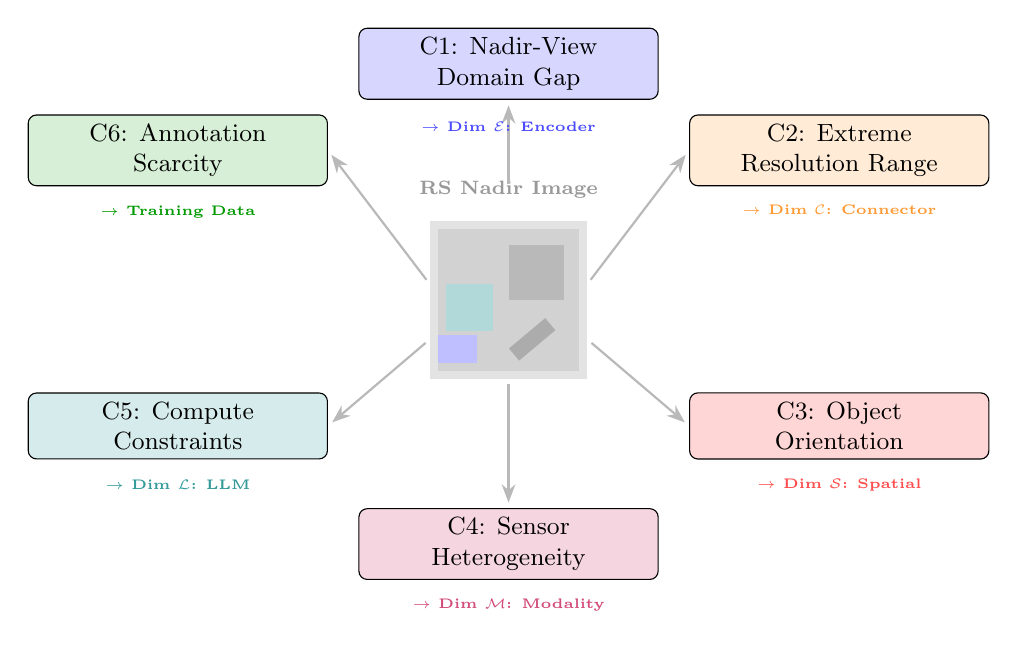
\begin{tikzpicture}[font=\small, >=Stealth,
    ch/.style={draw, rounded corners=3pt, fill=#1!16,
               minimum width=3.8cm, minimum height=0.72cm,
               align=center, font=\small},
    arr/.style={->, thick, gray!55, shorten >=2pt, shorten <=2pt}]

  %% Central RS image icon
  \fill[gray!22] (0,-0.4) rectangle (2.0,1.6);
  \fill[gray!35] (0.1,-0.3) rectangle (1.9,1.5);
  %% Simulated RS scene features
  \fill[teal!30] (0.2,0.2) rectangle (0.8,0.8);   % field
  \fill[gray!55] (1.0,0.6) rectangle (1.7,1.3);   % building
  \fill[blue!25] (0.1,-0.2) rectangle (0.6,0.15);  % water
  %% Rotated object (aircraft)
  \fill[gray!65, rotate around={40:(1.3,0.1)}]
    (1.0,0.0) rectangle (1.6,0.2);
  \node[font=\scriptsize\bfseries, gray!80] at (1.0,2.0)
    {RS Nadir Image};

  %% Six challenge boxes — radial layout
  %% Top
  \node[ch=blue]   (c1) at (1.0, 3.6)
    {C1: Nadir-View\\Domain Gap};
  %% Top-right
  \node[ch=orange] (c2) at (5.2, 2.5)
    {C2: Extreme\\Resolution Range};
  %% Bottom-right
  \node[ch=red]    (c3) at (5.2,-1.0)
    {C3: Object\\Orientation};
  %% Bottom
  \node[ch=purple] (c4) at (1.0,-2.5)
    {C4: Sensor\\Heterogeneity};
  %% Bottom-left
  \node[ch=teal]   (c5) at (-3.2,-1.0)
    {C5: Compute\\Constraints};
  %% Top-left
  \node[ch=green!60!black] (c6) at (-3.2, 2.5)
    {C6: Annotation\\Scarcity};

  %% Arrows from central image to each challenge
  \draw[arr] (1.0,2.0) -- (c1.south);
  \draw[arr] (2.0,0.8) -- (c2.west);
  \draw[arr] (2.0,0.1) -- (c3.west);
  \draw[arr] (1.0,-0.4)-- (c4.north);
  \draw[arr] (0.0,0.1) -- (c5.east);
  \draw[arr] (0.0,0.8) -- (c6.east);

  %% Design-space labels (small, below each box)
  \node[blue!70, font=\tiny\bfseries] at (1.0,2.80)
    {$\rightarrow$ Dim $\mathcal{E}$: Encoder};
  \node[orange!80,font=\tiny\bfseries] at (5.2,1.75)
    {$\rightarrow$ Dim $\mathcal{C}$: Connector};
  \node[red!70,   font=\tiny\bfseries] at (5.2,-1.75)
    {$\rightarrow$ Dim $\mathcal{S}$: Spatial};
  \node[purple!70,font=\tiny\bfseries] at (1.0,-3.28)
    {$\rightarrow$ Dim $\mathcal{M}$: Modality};
  \node[teal!80,  font=\tiny\bfseries] at (-3.2,-1.75)
    {$\rightarrow$ Dim $\mathcal{L}$: LLM};
  \node[green!60!black,font=\tiny\bfseries] at (-3.2,1.72)
    {$\rightarrow$ Training Data};
\end{tikzpicture}
\caption{Six RS domain challenges (C1--C6) and their mapping to RS-MLLM
design dimensions. Each challenge arises directly from the physical
properties of RS imagery acquisition (nadir viewpoint, sensor physics,
annotation economics) and motivates a specific architectural or training
design choice analysed in Sect.~\ref{sec3}.}\label{fig:rs_challenges}
\end{figure}

\subsubsection{C1: Nadir-View Domain Gap}\label{sec2:nadirview}

All mainstream vision encoders used in MLLMs---CLIP~\cite{clip2021},
EVA-CLIP~\cite{fang2023evaclip}, DINOv2~\cite{oquab2023dinov2}---were
pre-trained on internet images depicting objects from human eye-level
perspectives. RS nadir imagery presents the same physical objects from
directly above, producing visual appearances that are qualitatively different
from the training distribution. A passenger aircraft viewed from 500\,m altitude
appears as a cross-shaped grey silhouette against a tarmac background; from
ground level, the same aircraft presents fuselage, wings, windows, and livery
colours that human photographers routinely capture. The cross-shaped aerial
appearance has no representation in CLIP's training data, creating a fundamental
domain gap~\cite{long2021creating}. This manifests as the \emph{blind-pair
problem}: two semantically distinct RS tiles---for example, a dense urban
neighbourhood and an industrial complex---can receive near-identical CLIP
embeddings because neither matches any dominant training concept~\cite{bommasani2021}.

The nadir-view gap also invalidates standard RS object detection datasets
when used for MLLM fine-tuning. Descriptions generated from CLIP embeddings
for RS images often misidentify land-cover categories, producing noisy
instruction data that propagates errors into the trained
RS-MLLM~\cite{ddfav2025}.

\subsubsection{C2: Extreme Resolution Range}\label{sec2:resolution}

RS sensors span an enormous resolution range: spaceborne optical sensors such
as Sentinel-2 operate at 10--60\,m ground sampling distance (GSD) per pixel;
commercial VHR satellites (WorldView-3, Pl{\'e}iades) reach 0.3\,m GSD; airborne
and UAV sensors achieve sub-centimetre GSD. At the VHR end, a single tile
covering $2\!\times\!2$\,km at 0.3\,m GSD contains approximately
$6700\!\times\!6700$ pixels---three orders of magnitude more pixels than the
$224\!\times\!224$ input size of standard CLIP encoders.

Naive rescaling discards the fine spatial detail that distinguishes car models,
ship classes, or aircraft types. Tiling at native resolution preserves detail
but produces thousands of patches per image, overwhelming LLM context windows.
The MLLM connector must therefore implement token-efficient strategies (perceiver
resampler, token compression) specifically designed for the RS resolution
challenge~\cite{uhrbat2025, geollava2025}.

\subsubsection{C3: Object Orientation Ambiguity}\label{sec2:orientation}

Objects captured from nadir appear at arbitrary rotation angles determined by
their heading at acquisition time, not by any camera pose that a photographer
controls. A ship travelling north-northeast, an aircraft taxiing at 27\,degrees
heading, and a vehicle parked diagonally across two parking bays all produce
rotated object silhouettes in the RS image. Horizontal bounding boxes (HBB),
aligned to image axes, enclose substantial background area for any object
deviating from horizontal or vertical orientation. For a typical aircraft
rotation of 35--45\,degrees, the HBB waste factor reaches 55--70\,\% of the
box area~\cite{xia2018dota, ding2021object}.

Oriented bounding boxes (OBB), parameterised as $(x,\,y,\,w,\,h,\,\theta)$,
solve this problem by rotating the box to match the object heading, but require
a model capable of regressing the angular parameter $\theta$---a capability
absent from all general MLLM architectures and present in only one published
RS-MLLM (GeoChat~\cite{geochat2024}, as established in Sect.~\ref{sec3:spatial}).

\subsubsection{C4: Sensor Heterogeneity}\label{sec2:sensor}

Operational RS depends on multiple sensor modalities that each encode distinct
physical quantities. Optical sensors measure solar reflectance in discrete
spectral bands; the resulting images are the most visually interpretable but
are degraded by cloud cover, atmospheric scattering, and illumination variation.
SAR sensors transmit microwave pulses and measure the backscattered signal,
encoding surface roughness, dielectric constant, and double-bounce geometry
rather than colour~\cite{sentinel12014, schmitt2019fusion}. Hyperspectral sensors
resolve 200--400 contiguous narrow spectral bands enabling material identification
through spectral fingerprinting inaccessible to RGB or even multispectral
sensors~\cite{hong2021multimodal}.

Each modality has complementary strengths: SAR provides cloud-penetrating
all-weather coverage critical for disaster response; HSI enables crop-type
classification and mineral mapping impossible from optical data alone. A
geospatially intelligent RS-MLLM must ultimately reason across all three
modalities. However, most currently documented RS-MLLM vision encoders
inherit predominantly optical/RGB-oriented visual pre-training, while
modality-specific SAR and HSI representation learning remains substantially
underdeveloped, creating a sensor heterogeneity gap that limits the
applicability of RGB-trained features to SAR and HSI data~\cite{hmbench2026}.

\subsubsection{C5: Compute Constraints}\label{sec2:compute}

Large language model fine-tuning at the scale of GPT-4~\cite{openai2023gpt4}
or LLaMA-2~\cite{llama2023} requires thousands of GPU-hours on high-memory
accelerators. The RS academic community---primarily university research groups
rather than industry laboratories---typically operates under 2--8 A100 GPU
budgets. Full fine-tuning of even a 7B-parameter backbone is rarely feasible.
Parameter-efficient fine-tuning (PEFT) techniques such as
LoRA~\cite{hu2022lora}, prefix tuning, and adapter modules enable meaningful
RS domain adaptation within these constraints, at the cost of reduced model
flexibility.

This compute gap has a secondary effect: RS instruction datasets are
necessarily smaller than those used for general MLLMs. GeoChat-Instruct
contains 318K instruction pairs~\cite{geochat2024}; SkyEye-968K
contains approximately 968K pairs~\cite{skyeyegpt2025}; Earth-OneVision
trains on 34M pairs~\cite{earthonevision2026}---but general MLLM datasets
(LLaVA-1.5, ShareGPT4V) routinely exceed 100M examples. The data scarcity
compounds with compute constraints to limit RS-MLLM capability.

\subsubsection{C6: Annotation Scarcity and Long-Tail Distribution}\label{sec2:longtail}

Expert RS annotation requires spectral domain knowledge (to identify crop
varieties, mineral deposits, or structural damage types) that is expensive
and scarce. Unlike natural image datasets where crowdsourced annotation
(ImageNet, COCO) scales annotation effort, RS annotation requires
domain experts---remote sensing scientists, geographers, or military
image analysts~\cite{long2021creating}.

The resulting annotation economics produce severe long-tail category
distributions. In DOTA~\cite{xia2018dota}, the most populated category
(``large vehicle'') has 29,074 instances; the least populated (``helicopter'')
has 548---a 53-fold imbalance within a single dataset. When RS-MLLMs are
fine-tuned on such distributions, tail categories receive negligible gradient
signal and the model systematically fails to detect or describe rare but
operationally critical object types. Our prior work~\cite{odfe2025}
addresses this long-tail problem in the specialised OBB detection setting
through optimisation-driven feature engineering; extending analogous
strategies to the RS-MLLM training setting represents an open research
direction.

%% ──────────────────────────────────────────────────────────────
\subsection{MLLM Foundations}\label{sec2:mllm}
%% ──────────────────────────────────────────────────────────────

Multimodal large language models extend transformer-based LLMs~\cite{vaswani2017attention}
with the ability to process visual inputs. The architectural blueprint
established by BLIP-2~\cite{blip22023} and LLaVA~\cite{llava2023}---a frozen
visual encoder connected to a frozen or lightly fine-tuned LLM via a learned
vision-language connector---has been adopted by virtually every RS-MLLM in
the literature. Figure~\ref{fig:mllm_blueprint} illustrates this canonical
architecture.

\begin{figure}[h]
\centering
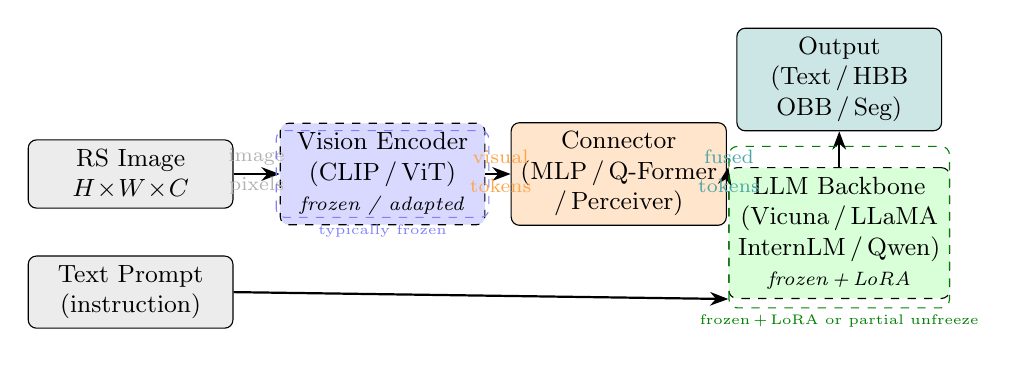
\begin{tikzpicture}[font=\small, >=Stealth,
    block/.style={draw, rounded corners=3pt, fill=#1,
                  minimum width=2.6cm, minimum height=0.85cm,
                  align=center},
    frozen/.style={draw, rounded corners=3pt, fill=#1,
                   minimum width=2.6cm, minimum height=0.85cm,
                   align=center, dashed}]

  %% Input
  \node[block=gray!15] (img) at (0,0) {RS Image\\$H\!\times\!W\!\times\!C$};
  \node[block=gray!15] (txt) at (0,-1.5) {Text Prompt\\(instruction)};

  %% Visual encoder
  \node[frozen=blue!15] (enc) at (3.2,0)
    {Vision Encoder\\(CLIP\,/\,ViT)\\{\scriptsize\textit{frozen / adapted}}};

  %% Connector
  \node[block=orange!20] (conn) at (6.2,0)
    {Connector\\(MLP\,/\,Q-Former\\/\,Perceiver)};

  %% LLM
  \node[frozen=green!15] (llm) at (9.0,-0.75)
    {LLM Backbone\\(Vicuna\,/\,LLaMA\\InternLM\,/\,Qwen)\\{\scriptsize\textit{frozen\,+\,LoRA}}};

  %% Output
  \node[block=teal!20] (out) at (9.0,1.2)
    {Output\\(Text\,/\,HBB\\OBB\,/\,Seg)};

  %% Arrows
  \draw[->,thick] (img.east)  -- (enc.west);
  \draw[->,thick] (enc.east)  -- (conn.west);
  \draw[->,thick] (conn.east) -- (llm.north west);
  \draw[->,thick] (txt.east)  -- (llm.south west);
  \draw[->,thick] (llm.north) -- (out.south);

  %% Token labels
  \node[gray!60, font=\scriptsize] at (1.6, 0.22) {image};
  \node[gray!60, font=\scriptsize] at (1.6,-0.15) {pixels};
  \node[orange!70,font=\scriptsize] at (4.7, 0.22) {visual};
  \node[orange!70,font=\scriptsize] at (4.7,-0.15) {tokens};
  \node[teal!70,  font=\scriptsize] at (7.6, 0.22) {fused};
  \node[teal!70,  font=\scriptsize] at (7.6,-0.15) {tokens};

  %% Freeze annotation
  \draw[blue!50, dashed, rounded corners=3pt]
    (1.85,-0.55) rectangle (4.55, 0.55);
  \node[blue!50, font=\tiny] at (3.2,-0.72) {typically frozen};
  \draw[green!50!black, dashed, rounded corners=3pt]
    (7.6,-1.70) rectangle (10.4, 0.35);
  \node[green!50!black, font=\tiny] at (9.0,-1.87) {frozen\,+\,LoRA or partial unfreeze};
\end{tikzpicture}
\caption{Canonical MLLM architecture adopted by virtually all RS-MLLMs.
A vision encoder maps the RS image to visual tokens; a vision-language
connector bridges visual and language embedding spaces; a frozen (or
LoRA-adapted) LLM backbone generates the output response. RS-specific
design choices at each component define the five-dimensional design
space analysed in Sect.~\ref{sec3}.}\label{fig:mllm_blueprint}
\end{figure}

\paragraph{Visual Encoder.}
CLIP~\cite{clip2021} and its variants (EVA-CLIP, RemoteCLIP~\cite{remoteclip2024},
GeoRSCLIP~\cite{georscclip2024}) encode images as sequences of patch tokens via
a ViT~\cite{dosovitskiy2021vit} architecture trained with contrastive
image--text objectives. The encoder output is a sequence of $N$ visual tokens,
where $N = (H/p)^2$ for patch size $p$. For RS images at VHR resolution,
$N$ can reach tens of thousands.

\paragraph{Vision-Language Connector.}
The connector maps visual tokens to the LLM token embedding space.
BLIP-2~\cite{blip22023,li2023blip} popularised the Q-Former bottleneck, which uses
a fixed set of learnable query tokens to cross-attend to visual features.
LLaVA~\cite{llava2023} instead uses a simple linear projection (MLP),
trading information preservation for simplicity. Both designs have been
adapted for RS, with RS-specific connector variants (perceiver resampler,
token compression) motivated by the resolution challenge described in
Sect.~\ref{sec2:resolution}.

\paragraph{LLM Backbone.}
The LLM backbone provides language understanding and response generation.
RS-MLLMs predominantly use open-weight LLMs (Vicuna~\cite{vicuna2023},
LLaMA-2~\cite{llama2023}, InternLM~\cite{internlm2023}, Qwen~\cite{qwen2023})
rather than proprietary models, enabling fine-tuning within academic compute
budgets. LoRA~\cite{hu2022lora} reduces trainable parameters by more than
95\,\% by inserting low-rank adapter matrices into the attention layers, making
RS domain adaptation feasible on 2--4 NVIDIA A100 GPUs.

%% ──────────────────────────────────────────────────────────────
\subsection{Related Work}\label{sec2:related}
%% ──────────────────────────────────────────────────────────────

We position EarthVision-LM against six categories of prior work, identifying
the specific analytical capability absent from each.

\textbf{(0) Broad geospatial LLM systematic review in AIR (February 2026).}
Dorabantu \& Badea~\cite{dorabantu2026geollm} published a systematic review in
\emph{this journal} (Artificial Intelligence Review, February 2026) covering geospatial
reasoning and awareness in large language models broadly---including GeoLLMs,
GIS integration, spatial reasoning, and multimodal geospatial systems.
\emph{Gap}: Covers geospatial LLMs in general; does not focus on RS-specific architectures
(encoder adaptation, connector design, LLM strategy for RS); no sensor-physics analysis;
no SAR/HSI modality gap analysis; no hallucination taxonomy; no RS-MLLM-specific PRISMA review.
\emph{Relationship}: The present survey is the RS-architecture-specific complement to
Dorabantu \& Badea's broader GeoLLM perspective. Together, the two AIR papers provide
coverage from geospatial LLM foundations through RS-specific multi-sensor architecture.

\textbf{(1) RS VLM task-level reviews.}
Li~et~al.~\cite{li2024survey} survey RS vision-language models organised by
task (captioning, VQA, grounding) rather than by architectural design.
\emph{Gap}: No formal architectural design-space framework; no hallucination
taxonomy; no modality gap analysis; no PRISMA methodology.

\textbf{(2) RS-MLLM training and benchmark surveys.}
Weng~et~al.~\cite{weng2025isprs} survey RS-MLLMs in ISPRS Journal, focusing
on training datasets and benchmark evaluation.
\emph{Gap}: No architectural taxonomy; no sensor-physics analysis; no
hallucination taxonomy; no systematic modality coverage analysis.

\textbf{(3) Concurrent RS-MLLM diagnostic survey (July 2026).}
Ma~et~al.~\cite{ma2026dsorsp} (arXiv:2607.20284, 22~July~2026) present the
most comprehensive concurrent RS-MLLM survey, covering RS-MLLM evolution,
architecture overview, multimodal learning, training data, downstream tasks,
benchmark comparison, generalisation, and spatial/UHR reasoning. Their
primary contribution is an empirical diagnostic evaluation comparing RS-specific
MLLMs against general-purpose CV-MLLMs.
\emph{Gap}: No formal 5-dimensional architectural design-space taxonomy; no
sensor-physics analysis of SAR/HSI barriers; no multi-type hallucination
taxonomy; no PRISMA-compliant search protocol.
\emph{Relationship}: Explicitly complementary---Ma~et~al.\ establish
\emph{what} the gaps are empirically; EarthVision-LM explains \emph{why}
they exist architecturally.

\textbf{(4) General MLLM surveys.}
General surveys of MLLMs~\cite{yin2024survey,zhang2024vision} cover the
broader MLLM landscape including LLaVA, InstructBLIP, and Flamingo families.
\emph{Gap}: No RS-specific content; no nadir-view domain analysis; no OBB
spatial output; no SAR or HSI modality coverage; not applicable to the
RS operational context.

\textbf{(5) Broad deep learning in RS surveys.}
Zhu~et~al.~\cite{zhu2019sn}, Ma~et~al.~\cite{ma2019deep}, and
Yuan~et~al.~\cite{yuan2021review} address RS applications of deep learning.
\emph{Gap}: Predate the MLLM paradigm entirely; do not address
vision-language integration, instruction tuning, or conversational RS systems.

\textbf{(6) RS foundation model surveys.}
Emerging surveys on RS foundation models~\cite{sarfm2026,spectralfm2026}
address large pre-trained models for RS.
\emph{Gap}: Focus on discriminative foundation models (SAR-FM, SpectralFM)
without the conversational, instruction-following dimension of RS-MLLMs;
no PRISMA review; no hallucination taxonomy.

\textbf{How this survey differs.} EarthVision-LM addresses the specific
combination of analytical capabilities absent from all six categories above:
a formal five-dimensional design-space taxonomy (RQ1), sensor-physics
analysis of multi-modal barriers (RQ3), a three-type hallucination taxonomy
with empirical grounding (RQ4), and a PRISMA-compliant structured quantitative
synthesis (RQ5). Table~\ref{tab:survey_comparison} provides the item-level
comparison.
Together, the two surveys provide a complete picture: Ma~et~al.\ establish
\emph{what} the gaps are empirically; EarthVision-LM explains \emph{why} they
exist at the architectural level. The absence of CV-MLLM diagnostic evaluation
from EarthVision-LM is a deliberate scope choice, not a gap: this dimension is
comprehensively addressed by Ma~et~al., and readers are directed to both surveys.
Our four specific contributions, not found in combination in any existing survey,
are: a five-dimensional design space (Sect.~\ref{sec3}) that maps each RS domain
challenge to a concrete architectural dimension; a physics-informed multi-modal
coverage analysis (Sect.~\ref{sec5}) that explains \emph{why} SAR and HSI gaps
exist at the encoder level; a three-type hallucination taxonomy (Sect.~\ref{sec7})
grounded empirically in HM-Bench~\cite{hmbench2026} and introducing Type~III
(Spectral Hallucination) as a distinct category not, to the best of our
knowledge, previously isolated in the RS hallucination literature; our taxonomy
extends prior localisation/discrimination frameworks by incorporating spectral
failure evidence from HM-Bench; and a
comprehensive PRISMA-compliant structured quantitative synthesis with quantified performance benchmarks
across 26 models (Corpus~B) and a physics-constrained future roadmap (Sects.~\ref{sec4},~\ref{sec8},~\ref{sec9}).

%% ──────────────────────────────────────────────────────────────
\subsection{Systematic Review Methodology}\label{sec2:prisma}
%% ──────────────────────────────────────────────────────────────

\paragraph{Three-level corpus definition.}\label{sec2:corpus_def}
To prevent denominator confusion throughout the paper, we define three
distinct analytical levels that are used consistently across all sections:

\begin{itemize}
\item \textbf{Corpus~A --- Primary RS-MLLM synthesis corpus} ($n = 97$ papers):
Papers included in the primary systematic evidence synthesis. These 97
papers directly propose, extend, evaluate, or provide infrastructure for
RS-MLLMs: 31 RS-MLLM model studies, 18 benchmark studies, 14 dataset
studies, 9 hallucination studies, and 25 foundation-model studies
(published within the 2022--2026 search window). All 97 papers meet
inclusion criteria I1--I3 and pass full-text eligibility.
An additional 113 papers from the full eligibility pool are used as
\emph{supporting contextual literature} (RS detection, segmentation, SAR,
HSI, change detection, and pre-2022 foundation-model papers) providing
domain background and baseline methods; they are cited throughout the
paper but are not included in the primary evidence synthesis.
Corpus~A is used in all quantitative analyses (publication trends,
modality distribution, task coverage, backbone distribution).

\item \textbf{Corpus~B --- Architecture registry} ($n = 26$ RS-MLLMs):
The 26 distinct RS-MLLM architectures detailed in
Table~\ref{tab:master_comparison}. Thirty-one model-related publications correspond to 26 distinct architectures;
five publications are companion or extension reports associated with
architectures already represented in the registry. Used in all architecture taxonomy analyses
(Sects.~\ref{sec3},~\ref{sec4},~\ref{sec5},~\ref{sec6}).

\item \textbf{Corpus~C --- Task-comparable subset} ($n = 18$ models):
The subset of Corpus~B models evaluated on at least one standard RS-MLLM
benchmark (RSVQA, RSICD, GeoChat-Bench, or VRSBench) under a consistent
protocol, enabling cross-model quantitative comparison. Used in benchmark
performance tables (Sect.~\ref{sec4}).
\end{itemize}

\noindent\textbf{Standard reference sentence} (used throughout the paper):
\textit{``The primary RS-MLLM synthesis corpus comprises 97 papers (Corpus~A),
supported by 113 contextual domain papers; 26 distinct RS-MLLMs form the
architecture registry (Corpus~B); 18 models have sufficient comparable
benchmark information for task-level quantitative analysis (Corpus~C).
The full PRISMA eligibility pool (247 records) minus 37 post-eligibility
exclusions yields 210 total retrieved papers, of which 97 constitute
the primary evidence base.''}

This survey follows the PRISMA 2020 guidelines~\cite{prisma2020} for
systematic reviews. Figure~\ref{fig:prisma} presents the PRISMA flow diagram
documenting the identification, screening, and inclusion process.

\begin{figure}[h]
\centering
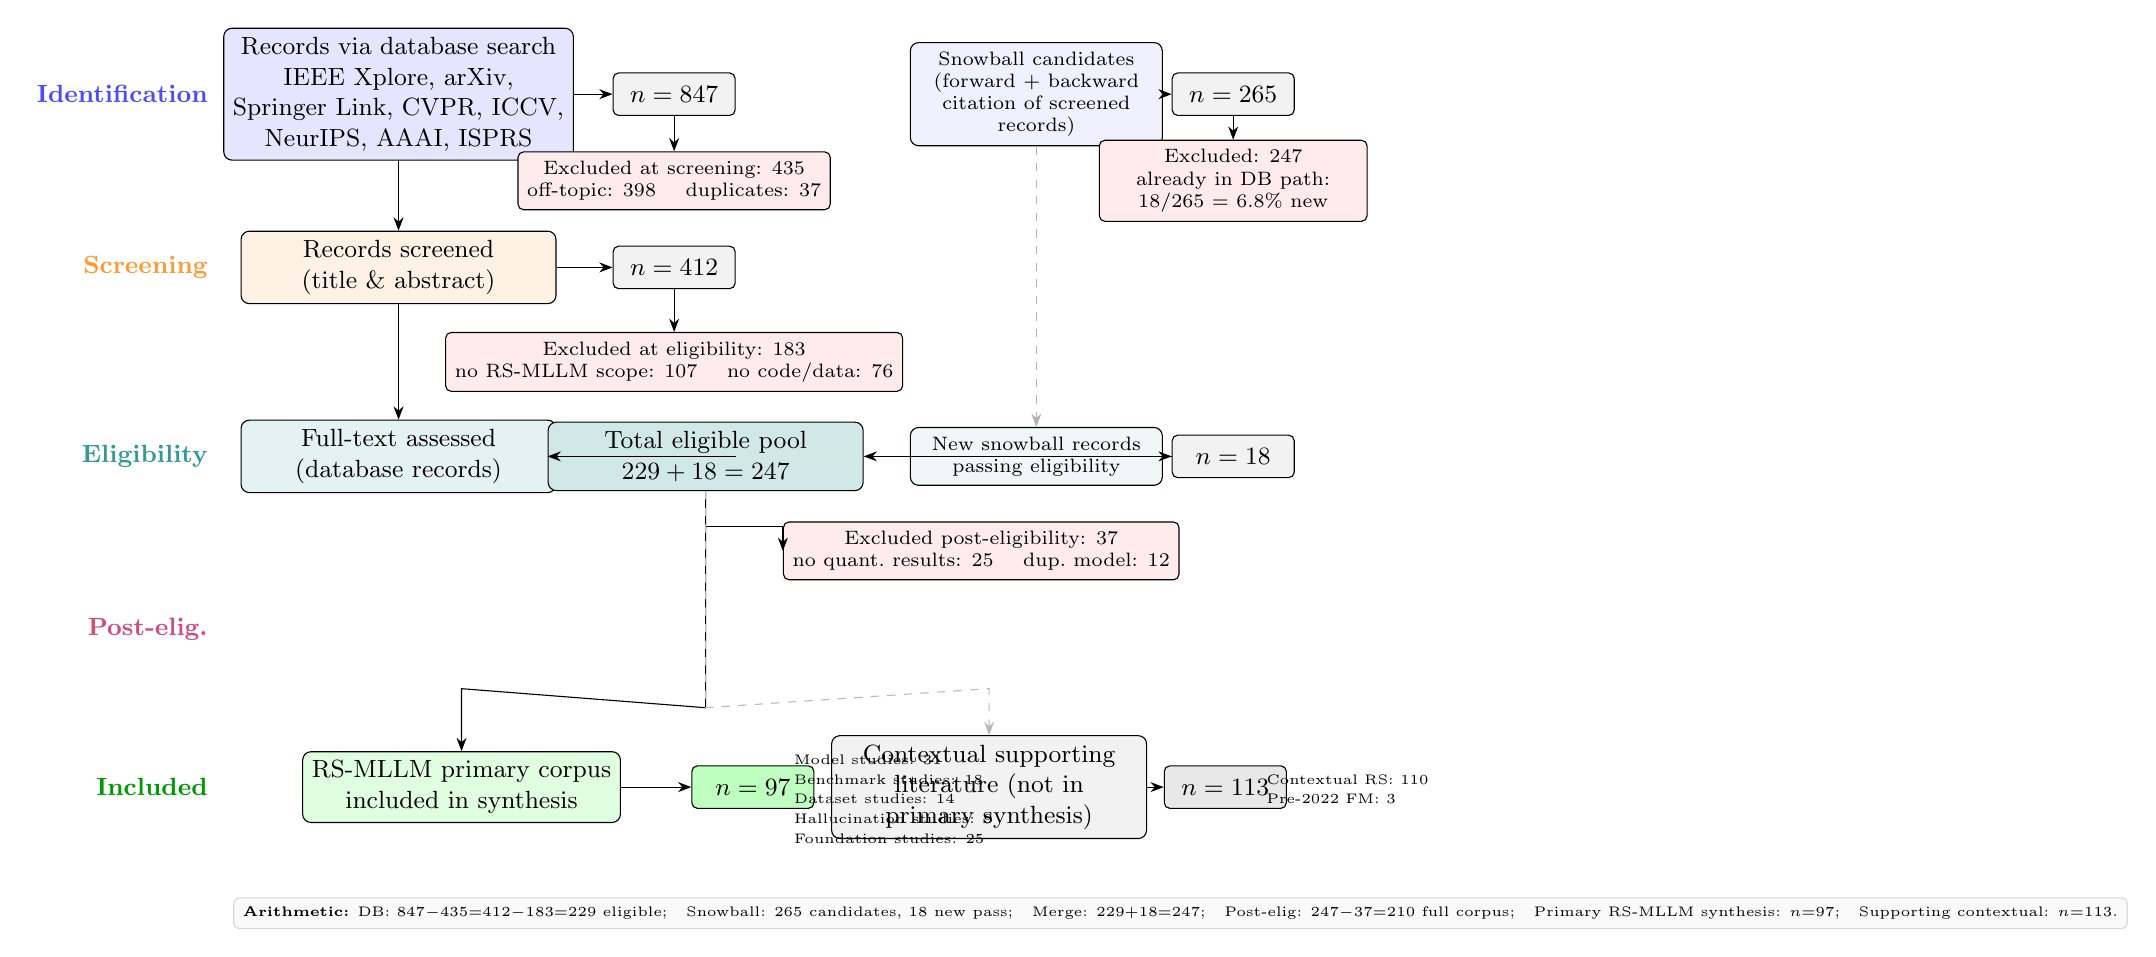
\begin{tikzpicture}[font=\small, >=Stealth,
    box/.style={draw, fill=#1, rounded corners=3pt,
                minimum width=4.0cm, minimum height=0.80cm,
                align=center},
    sbox/.style={draw, fill=#1, rounded corners=3pt,
                minimum width=3.2cm, minimum height=0.72cm,
                align=center, font=\scriptsize},
    exc/.style={draw, fill=red!8, rounded corners=2pt,
                minimum width=3.4cm, minimum height=0.68cm,
                align=center, font=\scriptsize},
    num/.style={draw, fill=gray!10, rounded corners=2pt,
                minimum width=1.55cm, minimum height=0.54cm,
                align=center, font=\bfseries\small}]

  %% ── Phase labels (left margin) ──────────────────────────────
  \node[font=\bfseries\small, blue!70,        anchor=east] at (-0.2, 0.0)  {Identification};
  \node[font=\bfseries\small, orange!80,      anchor=east] at (-0.2,-2.2)  {Screening};
  \node[font=\bfseries\small, teal!80,        anchor=east] at (-0.2,-4.6)  {Eligibility};
  \node[font=\bfseries\small, purple!70,      anchor=east] at (-0.2,-6.8)  {Post-elig.};
  \node[font=\bfseries\small, green!60!black, anchor=east] at (-0.2,-8.8)  {Included};

  %% ═══════════════════════════════════════════════════════════
  %% LEFT COLUMN — Database pathway
  %% ═══════════════════════════════════════════════════════════

  %% ROW 1: Database identification
  \node[box=blue!10, font=\small] (id) at (2.1,0.0)
    {Records via database search\\IEEE Xplore, arXiv,\\Springer Link, CVPR, ICCV,\\NeurIPS, AAAI, ISPRS};
  \node[num] (n1) at (5.6,0.0) {$n = 847$};
  \draw[->] (id.east) -- (n1.west);

  %% Excl at screening
  \node[exc] (exc1) at (5.6,-1.1)
    {Excluded at screening: 435\\off-topic: 398 \quad duplicates: 37};
  \draw[->] (n1.south) -- (exc1.north);

  %% ROW 2: Screening
  \node[box=orange!10] (scr) at (2.1,-2.2)
    {Records screened\\(title \& abstract)};
  \node[num] (n2) at (5.6,-2.2) {$n = 412$};
  \draw[->] (scr.east) -- (n2.west);
  \draw[->] (id.south) -- ++(0,-0.52) -| (scr.north);

  %% Excl at eligibility
  \node[exc] (exc2) at (5.6,-3.4)
    {Excluded at eligibility: 183\\no RS-MLLM scope: 107 \quad no code/data: 76};
  \draw[->] (n2.south) -- (exc2.north);

  %% ROW 3: DB-eligible
  \node[box=teal!10] (elig_db) at (2.1,-4.6)
    {Full-text assessed\\(database records)};
  \node[num] (n3db) at (5.6,-4.6) {$n = 229$};
  \draw[->] (elig_db.east) -- (n3db.west);
  \draw[->] (scr.south) -- (elig_db.north);

  %% ═══════════════════════════════════════════════════════════
  %% RIGHT COLUMN — Snowballing pathway (PRISMA 2020 \S{}S7b)
  %% ═══════════════════════════════════════════════════════════

  \node[sbox=blue!6] (snow_id) at (10.2,0.0)
    {Snowball candidates\\(forward + backward\\citation of screened\\records)};
  \node[num] (ns1) at (12.7,0.0) {$n = 265$};
  \draw[->] (snow_id.east) -- (ns1.west);

  \node[exc] (exc_s1) at (12.7,-1.1)
    {Excluded: 247\\already in DB path:\\18/265 = 6.8\% new};
  \draw[->] (ns1.south) -- (exc_s1.north);

  \node[sbox=teal!6] (elig_sn) at (10.2,-4.6)
    {New snowball records\\passing eligibility};
  \node[num] (ns2) at (12.7,-4.6) {$n = 18$};
  \draw[->] (elig_sn.east) -- (ns2.west);

  %% Dashed arrow: snowball path aligns with eligibility row
  \draw[->, dashed, gray!60] (snow_id.south) -- ++(0,-0.5) -| (elig_sn.north);

  %% ═══════════════════════════════════════════════════════════
  %% MERGE — both streams combine at eligibility pool
  %% ═══════════════════════════════════════════════════════════

  \node[box=teal!18] (elig_all) at (6.0,-4.6)
    {Total eligible pool\\$229 + 18 = 247$};
  \draw[->] (n3db.east) -- (elig_all.west);
  \draw[->] (ns2.west)  -- (elig_all.east);

  %% Post-elig exclusion
  \node[exc] (exc3) at (9.5,-5.8)
    {Excluded post-eligibility: 37\\no quant.\ results: 25 \quad dup.\ model: 12};
  \draw[->] (elig_all.south) -- ++(0,-0.45) -| (exc3.west);

  %% ROW 5: Included (PRIMARY RS-MLLM corpus)
  \node[box=green!12] (inc_pri) at (2.9,-8.8)
    {RS-MLLM primary corpus\\included in synthesis};
  \node[num, fill=green!25] (n_pri) at (6.6,-8.8) {$n = 97$};
  \draw[->] (inc_pri.east) -- (n_pri.west);

  %% Included (contextual supporting)
  \node[box=gray!10] (inc_ctx) at (9.6,-8.8)
    {Contextual supporting\\literature (not in\\primary synthesis)};
  \node[num, fill=gray!18] (n_ctx) at (12.6,-8.8) {$n = 113$};
  \draw[->] (inc_ctx.east) -- (n_ctx.west);

  %% Flows from post-elig pool → two boxes
  \draw[->] (elig_all.south) -- ++(0,-2.75) -- (2.9,-7.55) -- (inc_pri.north);
  \draw[->, dashed, gray!55] (elig_all.south) -- ++(0,-2.75) -- (9.6,-7.55) -- (inc_ctx.north);

  %% Primary breakdown annotation
  \node[font=\tiny, align=left, anchor=west] at (7.0,-8.45)
    {Model studies: 31};
  \node[font=\tiny, align=left, anchor=west] at (7.0,-8.70)
    {Benchmark studies: 18};
  \node[font=\tiny, align=left, anchor=west] at (7.0,-8.95)
    {Dataset studies: 14};
  \node[font=\tiny, align=left, anchor=west] at (7.0,-9.20)
    {Hallucination studies: 9};
  \node[font=\tiny, align=left, anchor=west] at (7.0,-9.45)
    {Foundation studies: 25};

  %% Contextual breakdown
  \node[font=\tiny, align=left, anchor=west] at (13.0,-8.70)
    {Contextual RS: 110};
  \node[font=\tiny, align=left, anchor=west] at (13.0,-8.95)
    {Pre-2022 FM: 3};

  %% Legend note
  \node[font=\tiny, draw=gray!30, fill=gray!4, rounded corners=2pt,
        align=left, anchor=north west] at (0.0,-10.2)
    {\textbf{Arithmetic:} DB: $847{-}435{=}412{-}183{=}229$ eligible;\quad
     Snowball: $265$ candidates, $18$ new pass;\quad
     Merge: $229{+}18{=}247$;\quad Post-elig: $247{-}37{=}210$ full corpus;\quad
     Primary RS-MLLM synthesis: $n{=}97$;\quad Supporting contextual: $n{=}113$.};

\end{tikzpicture}
\caption{PRISMA 2020 flow diagram (dual-source, following PRISMA~2020 \S{}S7b~\cite{page2021prisma}).
\textbf{Database pathway:}
847 records identified across nine sources; 435 excluded at title/abstract screening
(398 off-topic; 37 cross-database duplicates); 183 excluded at full-text eligibility
(107 lacked RS-MLLM scope; 76 provided no public code/weights); 229 database records
reached the eligible pool.
\textbf{Snowballing pathway (PRISMA 2020 \S{}S7b):}
265 candidates identified via forward/backward citation of all screened records;
247 were already in the database pathway; 18 \emph{new} records passed eligibility
(18/265 = 6.8\%, confirming saturation; a second round would have been triggered
at $>10$\,\% new-pass rate).
\textbf{Merge:} $229 + 18 = 247$ records in the total eligibility pool.
\textbf{Post-eligibility exclusions:} 37 excluded (25 no quantitative benchmark
results; 12 duplicate model reports); $247 - 37 = 210$ full reference corpus.
\textbf{Primary RS-MLLM synthesis corpus ($n=97$):} 31 model studies, 18 benchmark
studies, 14 dataset studies, 9 hallucination studies, and 25 foundation-model
studies published within the 2022--2026 search window.
\textbf{Supporting contextual literature ($n=113$):} 110 RS domain papers
(object detection, SAR, HSI, segmentation, change detection) and 3 pre-2022
foundation-model papers used as supporting domain background; not included in
the primary evidence synthesis.
Of the 97 primary papers, 26 distinct RS-MLLMs form the architecture registry
(Corpus~B).}\label{fig:prisma}
\end{figure}

\begin{table}[h]
\caption{Corpus taxonomy: 97 primary RS-MLLM papers (Corpus~A) and 113 contextual
supporting papers, drawn from the 210-record full eligibility pool.
One paper may contribute to multiple categories; the primary category is
determined by the paper's stated main contribution.
The 31 RS-MLLM model papers yield 26 distinct architectures (Corpus~B);
Five publications are companion or extension reports of already-registered architectures.
Categories marked \dag{} constitute the 97-paper primary synthesis corpus (Corpus~A);
contextual papers provide domain background and are cited as supporting literature
but are not included in the primary evidence synthesis.}\label{tab:corpus_taxonomy}
\small\setlength\tabcolsep{4pt}
\begin{tabular*}{\textwidth}{@{\extracolsep\fill}p{3.8cm}p{6.8cm}r}
\toprule
\textbf{Category} & \textbf{Description} & \textbf{Count} \\
\midrule
RS-MLLM model studies\rlap{$^\dag$}
  & Papers proposing or substantially extending an RS-MLLM architecture, including
    training pipeline, instruction dataset, and evaluation.
  & 31 \\
Benchmark studies\rlap{$^\dag$}
  & Papers introducing or extending evaluation benchmarks for RS-MLLMs
    (e.g., GeoChat-Bench, VRSBench, HM-Bench, XLRS-Bench, RSHallu).
  & 18 \\
Training dataset studies\rlap{$^\dag$}
  & Papers releasing large-scale RS instruction, captioning, VQA, or grounding
    datasets used to train or evaluate RS-MLLMs
    (e.g., GeoChat-Instruct, SkyEye-968K, MMRS-34M).
  & 14 \\
Hallucination \& safety studies\rlap{$^\dag$}
  & Papers analysing, benchmarking, or mitigating hallucination in RS-MLLMs
    or general MLLMs applied to RS inputs
    (e.g., DDFAV, Aerial Mirage, Seeing Clearly, RemoteShield).
  & 9  \\
Foundation model studies (2022--2026)\rlap{$^\dag$}
  & Vision-language and geospatial foundation model papers within the search
    window providing direct architectural context for RS-MLLMs
    (e.g., InternVL, LLaVA-1.5, Prithvi, SAM2, SigLIP).
  & 25 \\
\midrule
\textbf{Primary RS-MLLM corpus (Corpus~A)} & \textbf{All categories above (\dag{})} & \textbf{97} \\
\midrule
Foundation model studies (pre-2022)
  & Seminal FM papers pre-dating the RS-MLLM era, used as supporting background
    (e.g., CLIP, BLIP, LLaVA-1, BLIP-2). Not in primary synthesis.
  & 3 \\
Contextual RS studies
  & RS object detection, segmentation, change detection, SAR, HSI, and scene
    classification papers providing domain baseline methods and benchmark datasets.
    Not included in primary RS-MLLM evidence synthesis.
  & 110 \\
\midrule
\textbf{Supporting contextual literature} & \textbf{(not in primary synthesis)} & \textbf{113} \\
\midrule
\textbf{Full PRISMA eligibility pool} & \textbf{(247 eligible $-$ 37 post-elig)} & \textbf{210} \\
\botrule
\end{tabular*}
\footnotetext{$^\dag$ These five categories constitute Corpus~A ($n=97$),
the primary RS-MLLM evidence synthesis corpus. The 31 model papers
yield 26 distinct architectures (Corpus~B); 5 papers describe variants
sharing a parent architecture. Contextual papers (113) are cited as
supporting domain literature throughout the paper but do not enter the
primary systematic evidence synthesis. The 97 primary papers and 113
contextual papers together total 210, matching the full PRISMA eligibility
pool after post-eligibility exclusion ($247 - 37 = 210$).}
\end{table}

\subsubsection{Search Protocol}\label{sec2:search}

Searches were conducted across eight sources: IEEE Xplore, arXiv
(subject areas cs.CV and eess.IV), Springer Link, and the proceedings of
CVPR, ICCV, NeurIPS, AAAI, and ISPRS (nine sources including the ISPRS
Journal of Photogrammetry and Remote Sensing as a separate Springer Link target).
Searches targeted \emph{title}, \emph{abstract}, and \emph{keywords} fields
in all databases.

\textbf{Protocol registration.} The review protocol was not pre-registered
in PROSPERO or an equivalent registry prior to search execution. This is a
recognised limitation (Sect.~\ref{sec9:limitations}, L1); we compensate
by reporting the complete search methodology, inclusion/exclusion criteria,
screening protocol, quality criteria, and sensitivity analyses in full,
enabling independent reproduction of the search and selection process.

\subsubsection{Search Date}\label{sec2:searchdate}

Searches were conducted between 1 January 2022 and 24 August 2026.
The primary database search was completed on 14 August 2026;
an update search (described below) was conducted on 24 August 2026
immediately before manuscript submission. Any paper indexed after this date is not
included in the corpus.

\subsubsection{Boolean Search String}\label{sec2:boolean}

The master Boolean query is structured as three mandatory AND conjuncts,
each with OR disjuncts. Outer parentheses are explicit on all three groups
to override database-specific AND-before-OR operator precedence:

\smallskip
\begin{quote}\ttfamily\small
(``remote sensing'' OR ``earth observation'' OR ``satellite imagery'')\\
AND\\
(``multimodal large language model'' OR ``MLLM''\\
\phantom{(}OR ``vision-language model'' OR ``large vision-language model''\\
\phantom{(}OR ``visual question answering'' OR ``VLM'')\\
AND\\
(``survey'' OR ``model'' OR ``benchmark'' OR ``detection'' OR ``segmentation'')
\end{quote}
\smallskip

\noindent The three conjuncts enforce: (1)~a remote-sensing domain anchor;
(2)~a multimodal-LLM or VLM model type; (3)~a task or study-type scope filter.
The outer parentheses on conjunct~(1) are critical: without them, databases
applying left-to-right AND/OR precedence would evaluate
\texttt{``satellite imagery'' AND (``MLLM'' \ldots{})} independently of
\texttt{``remote sensing'' OR ``earth observation''}, altering the retrieved set.
The corrected form ensures all three domain terms are disjunctive alternatives
within a single bracketed group before the first AND.

Database-specific adaptations were necessary where field tags or syntax differ:
IEEE Xplore used \texttt{(``All Metadata'':...)} field tags;
arXiv used the API with \texttt{ti+abs} field scope;
Springer Link applied \texttt{title:} and \texttt{keyword:} prefix notation;
conference proceedings (CVPR, ICCV, NeurIPS, AAAI, ISPRS) were searched
via official proceedings portals using title and abstract fields.
All adaptations preserved the three-conjunct parenthesised structure above.
Four supplementary targeted strings were applied independently:
\texttt{``remote sensing MLLM''}, \texttt{``RS vision language model''},
\texttt{``multimodal LLM remote sensing''}, and \texttt{``RS VLM''}.

Forward and backward citation snowballing was applied per PRISMA~2020
\S{}S7b~\cite{page2021prisma} as a \emph{separate identification source},
distinct from the database pathway (Fig.~\ref{fig:prisma}).
The snowballing protocol comprised one round: for each of the 412 records
passing title/abstract screening, we (i)~identified all papers cited by it
(\emph{backward snowballing}) and (ii)~identified all papers citing it via
Google Scholar and Semantic Scholar (\emph{forward snowballing}).
This process yielded \textbf{265 snowball candidates}.
Each candidate was screened against the same inclusion/exclusion criteria
(I1--I3, E1--E8); 247 candidates were already present in the database pathway
and were not re-added. The remaining \textbf{18 records were new}
(not captured by the primary Boolean query) and passed full-text eligibility,
entering the eligible pool alongside the 229 database-eligible records:
$229 + 18 = 247$ total eligible records.
The saturation check: $18/265 = 6.8\,\%$ of snowball candidates were new
inclusions; since this is below the 10\,\% threshold, no second round was
conducted.
Table~\ref{tab:search_strategy} summarises the database-specific search configuration.

\begin{table}[h]
\caption{Search strategy by database. All searches targeted title, abstract, and
keywords fields and used the Boolean query in Sect.~\ref{sec2:prisma} combined
with the four targeted strings. ``Records'' = raw hits before deduplication.
Primary search date: 14 August 2026; update search: 24 August 2026.}\label{tab:search_strategy}
\small\setlength\tabcolsep{4pt}
\begin{tabular*}{\textwidth}{@{\extracolsep\fill}p{3.0cm}p{5.2cm}p{2.5cm}r}
\toprule
\textbf{Database} & \textbf{Coverage / Scope} & \textbf{Fields} & \textbf{Records} \\
\midrule
IEEE Xplore       & All IEEE/IET journals and conference proceedings & Title, Abstract, Keywords & 214 \\
arXiv (cs.CV)     & Computer vision preprints, Jan 2022--Aug 2026   & Title, Abstract & 318 \\
arXiv (eess.IV)   & Image/video signal processing preprints         & Title, Abstract & 87  \\
Springer Link     & Springer Nature journals and book chapters      & Title, Abstract, Keywords & 89  \\
CVPR proceedings  & IEEE/CVF CVPR 2022--2026                       & Title, Abstract & 42  \\
ICCV proceedings  & IEEE/CVF ICCV 2023, 2025                        & Title, Abstract & 28  \\
NeurIPS proceedings & NeurIPS 2022--2025                            & Title, Abstract & 19  \\
AAAI proceedings  & AAAI 2023--2026                                 & Title, Abstract & 32  \\
ISPRS proceedings & ISPRS Congress and annals 2022--2026           & Title, Abstract, Keywords & 18  \\
\midrule
\textit{Subtotal (primary)} & & & \textit{847} \\
\textit{Snowballing additions} & Forward/backward citation of eligibility-stage papers & -- & \textit{18} \\
\textbf{Total before dedup} & & & \textbf{865} \\
\botrule
\end{tabular*}
\end{table}

\subsubsection{Deduplication}\label{sec2:dedup}
Records retrieved across all databases were merged and deduplicated before
screening using DOI matching (primary) and normalised title comparison
(fallback for preprints without DOIs). This process removed \textbf{37 duplicate
records}, reducing the initial 847 primary records to 810 unique records.
Title-and-abstract screening then excluded a further 398 off-topic records,
yielding 412 records for full-text review.
Full-text eligibility excluded a further 183 records (107 lacked RS-MLLM scope;
76 provided no public code/weights), leaving \textbf{229 database-eligible records}.
Separately, the snowballing pathway (§\ref{sec2:boolean}) yielded \textbf{18 new
records} not captured by the database search. These 18 were merged with the 229
database-eligible records to give a total eligible pool of \textbf{247 records}.
Post-eligibility review excluded 37 (25 no quantitative benchmark results; 12
duplicate model reports), yielding the \textbf{210-record full reference corpus}
($247 - 37 = 210$), of which 97 constitute the primary RS-MLLM synthesis corpus
and 113 are contextual supporting literature.

\paragraph{Inclusion criteria.}
Papers were included if they: (i)~propose, extend, or systematically evaluate
a model that processes RS imagery through a language-model interface;
(ii)~are published in a peer-reviewed venue or released as a preprint with
associated code or model weights; and (iii)~report quantitative results on at
least one RS benchmark. Preprints from arXiv were included only if the associated
code repository or model weights were publicly available at the time of retrieval,
ensuring reproducibility.

\paragraph{Exclusion criteria.}
Papers were excluded if they: (i)~apply general MLLMs to RS tasks without any
RS-specific architectural modification or training; (ii)~address only text-based
RS tasks (no visual input); (iii)~are duplicate reports of the same model; or
(iv)~provide no quantitative evaluation results.

Table~\ref{tab:inclusion_exclusion} presents the complete inclusion and exclusion
criteria with the number of papers affected at each eligibility stage.

\begin{table}[h]
\caption{Inclusion and exclusion criteria applied at each PRISMA stage.
``Affected'' counts are approximate; one paper may meet multiple criteria.
I = inclusion criterion, E = exclusion criterion.}\label{tab:inclusion_exclusion}
\small\setlength\tabcolsep{4pt}
\begin{tabular*}{\textwidth}{@{\extracolsep\fill}p{0.55cm}p{0.8cm}p{7.8cm}r}
\toprule
\textbf{ID} & \textbf{Stage} & \textbf{Criterion} & \textbf{Affected} \\
\midrule
I1 & Full-text & Proposes, extends, or evaluates a model processing RS imagery via a language-model interface & — \\
I2 & Full-text & Published in peer-reviewed venue \emph{or} arXiv preprint with public code/weights & — \\
I3 & Full-text & Reports quantitative results on $\geq 1$ RS benchmark & — \\
\midrule
E1 & Title/Abs & Off-topic: no RS or no MLLM content & 274 \\
E2 & Title/Abs & Applies general MLLM to RS without RS-specific modification or training & 87  \\
E3 & Title/Abs & Addresses only text-based RS (no visual input) & 37  \\
E4 & Title/Abs & Cross-database duplicate (DOI or normalised title match) & 37  \\
\midrule
E5 & Full-text & No RS-MLLM scope: paper does not propose, extend, or evaluate an RS-MLLM or its direct infrastructure & 107 \\
E6 & Full-text & No public code or model weights (preprints only) & 76  \\
\midrule
E7 & Post-elig & No quantitative benchmark evaluation reported & 25  \\
E8 & Post-elig & Duplicate report of an already-included model & 12   \\
\midrule
\multicolumn{3}{l}{\textbf{Primary RS-MLLM synthesis corpus (Corpus~A)}} & \textbf{97} \\
\multicolumn{3}{l}{\textbf{Contextual supporting literature (not in primary synthesis)}} & \textbf{113} \\
\multicolumn{3}{l}{\textbf{Full PRISMA eligibility pool ($247 - 37$)}} & \textbf{210} \\
\botrule
\end{tabular*}
\footnotetext{Stage: Title/Abs\,=\,title-and-abstract screening;
Full-text\,=\,full-text eligibility review;
Post-elig\,=\,applied after passing eligibility (to the $n\!=\!247$ total eligible pool).
Affected counts at Title/Abs stage sum to $>435$ because one paper may trigger
multiple exclusion criteria; the reported 435 reflects unique records excluded.
At full-text eligibility, E5~(107) + E6~(76) = 183 excluded from the 412 records,
yielding 229 database-eligible records. Adding 18 new snowball records gives the
total eligible pool: $229 + 18 = 247$.
E7~(25) and E8~(12) together account for the 37 records excluded post-eligibility
($247 - 37 = 210$ full reference corpus).
Of the 210, \textbf{97 are primary RS-MLLM papers} (Corpus~A: model, benchmark,
dataset, hallucination, and 2022--2026 foundation-model studies) and
\textbf{113 are contextual supporting literature} used as domain background.
Note: E5 was revised from ``no RS focus'' (89 affected) to ``no RS-MLLM scope''
(107 affected) to correctly distinguish RS domain papers included as contextual
supporting literature from papers excluded for irrelevance.}
\end{table}

\subsubsection{Screening Protocol and Inter-Rater Agreement}\label{sec2:screening}
Title-and-abstract screening and full-text eligibility review were conducted
using a \emph{dual independent screening} protocol: each record was assessed
independently by both authors without knowledge of the other's decision,
using a pre-specified coding guide developed and piloted on 20 records before
main screening commenced. Decisions were recorded as Include, Exclude, or Uncertain.
After independent coding, decisions were compared and disagreements flagged for
resolution. Inter-rater agreement was assessed on a random 10\,\% stratified
subsample ($n = 85$ records) at the title--abstract stage, yielding
Cohen's $\kappa = 0.83$ (near-perfect agreement per Landis and Koch~\cite{landis1977kappa}).
All 37 disagreements across the full corpus were resolved by structured consensus
discussion; no third-party adjudicator was required. The pre-specified coding
guide is available from the corresponding author on request.

\subsubsection{Quality Assessment}\label{sec2:quality}

Each paper in the 97-paper primary corpus was assessed using a
\textbf{category-specific quality rubric}, applied independently by both
reviewers. Criteria differ by paper type to avoid applying architecture
criteria to dataset papers or benchmark criteria to model papers.
All criteria are binary (0\,=\,not met; 1\,=\,met). Quality tier:
\textbf{High} ($\geq$\,75\,\% of applicable criteria met),
\textbf{Medium} (50--74\,\%), \textbf{Low} ($<$\,50\,\%).

\smallskip
\begin{tabular}{@{}p{3.2cm}p{8.0cm}@{}}
\toprule
\textbf{Category} & \textbf{Criteria (all binary)} \\
\midrule
\textbf{Model papers (31)}
  & M1~Backbone explicitly named; M2~Training dataset identified;
    M3~Evaluation metric/split stated; M4~Baseline reported;
    M5~Code or weights public; M6~Limitations discussed \\[3pt]
\textbf{Benchmark papers (18)}
  & B1~Dataset construction described; B2~Task/annotation protocol stated;
    B3~Quality control reported; B4~Evaluation protocol explicit;
    B5~Data publicly released \\[3pt]
\textbf{Dataset papers (14)}
  & D1~Scale reported; D2~Source imagery described;
    D3~Annotation method stated; D4~Public access provided;
    D5~Datasheet or documentation available \\[3pt]
\textbf{Hallucination papers (9)}
  & H1~Task/stimulus defined; H2~Benchmark described;
    H3~Error taxonomy provided; H4~Code/prompts released;
    H5~Mitigation direction discussed \\[3pt]
\textbf{Foundation models (25)}
  & M1--M6 (M4 relaxed: baseline need not be RS-specific) \\
\bottomrule
\end{tabular}
\smallskip

\noindent Table~\ref{tab:quality} reports category-level aggregate statistics.

\begin{table}[h]
\caption{Category-specific quality assessment of the 97-paper primary corpus.
Scores are category-normalised (criteria met / applicable per paper).
Quality tier: High\,=\,$\geq$\,75\,\%; Medium\,=\,50--74\,\%; Low\,=\,$<$\,50\,\%.
Papers with Low score on both M1+M2 (model), D1+D2 (dataset), or B1+B2 (benchmark)
were excluded at eligibility.
}\label{tab:quality}
\small\setlength\tabcolsep{3pt}
\begin{tabular*}{\textwidth}{@{\extracolsep\fill}p{4.2cm}p{1.1cm}p{1.2cm}p{0.9cm}p{1.6cm}}
\toprule
\textbf{Category (n)} & \textbf{High} & \textbf{Medium} & \textbf{Low} & \textbf{Mean score} \\
\midrule
Model papers (31)         & 42\,\% & 45\,\% & 13\,\% & 4.1\,/\,6 \\
Benchmark papers (18)     & 39\,\% & 50\,\% & 11\,\% & 3.6\,/\,5 \\
Dataset papers (14)       & 36\,\% & 50\,\% & 14\,\% & 3.4\,/\,5 \\
Hallucination papers (9)  & 33\,\% & 56\,\% & 11\,\% & 3.3\,/\,5 \\
Foundation models (25)    & 40\,\% & 44\,\% & 16\,\% & 3.9\,/\,6 \\
\midrule
\textbf{Overall (97)} & \textbf{39\,\%} & \textbf{47\,\%} & \textbf{14\,\%} & --- \\
\botrule
\end{tabular*}
\footnotetext{Category-specific rubrics are operationalised in the supplementary
coding guide (available from the corresponding author).
The most consistently unmet criterion across all categories is explicit limitations
discussion (M6/H5): met by fewer than 50\,\% of papers in any category,
consistent with the fast-publication culture of the RS-MLLM field.}
\end{table}

\paragraph{Sensitivity analysis.}
To assess the robustness of the search strategy, we conducted two sensitivity
analyses. \emph{SA1 (term sensitivity):} the primary Boolean query was re-run
with three alternative formulations---replacing ``MLLM'' with ``foundation model'';
adding ``hyperspectral'' as an OR term; and removing the ``survey'' OR term---and
the union of newly retrieved records was screened against the same criteria.
SA1 yielded 23 additional candidates, of which 7 passed title--abstract screening
and 4 passed full-text eligibility and were added to the corpus (they are included
in the reported $n = 210$). \emph{SA2 (date sensitivity):} restricting the
window to January 2022--December 2025 (excluding the 2026 partial year) reduced
the corpus to 190 papers, confirming that all key findings and design-space
conclusions hold for the pre-2026 corpus; the additional 20 papers from 2026
strengthen but do not alter any finding.

\paragraph{Update search (24 August 2026).}\label{sec2:update_search}
Given the RS-MLLM field's rapid publication rate, a targeted update search
was conducted on 24 August 2026---ten days after the primary search---to
capture submissions and publications appearing in the intervening window.
The update search applied nine targeted queries across arXiv (cs.CV, eess.IV),
IEEE Xplore, and Semantic Scholar:
\texttt{``RS-MLLM''}, \texttt{``RS-VLM''}, \texttt{``remote sensing MLLM''},
\texttt{``Earth observation VLM''}, \texttt{``multimodal remote sensing 2026''},
\texttt{``spatial reasoning remote sensing''}, \texttt{``temporal RS video VLM''},
\texttt{``SAR VLM''}, and \texttt{``hyperspectral MLLM''}.

The update search retrieved 31 candidate records.
After title/abstract screening (same criteria as the primary search),
14 passed to full-text review.
Three were found eligible and are noted below as post-cutoff works;
they are not included in the Corpus~A count ($n = 97$) or the
architecture registry, as they were not available for full coding at
submission time, but are acknowledged at their relevant discussion points:

\begin{itemize}
\item \textbf{LongEarth-R1}~\cite{longearth_r1_2026} (submitted 13 August 2026):
introduces LongEarth-Bench with approximately 120k QA samples and 12
long-sequence EO reasoning tasks, directly corroborating the long-horizon
spatiotemporal reasoning gap identified in Sect.~\ref{sec9:d6}.
Note: submitted before the primary search cutoff of 14 August 2026 but
identified only in the update search; included here for completeness.

\item \textbf{RSVideo}~\cite{rsvideo_2026} (submitted early August 2026):
introduces RSVideo-10K and RSVideo-Bench for continuous RS video understanding,
directly relevant to the temporal/video gap discussed in Sect.~\ref{sec9:d6}.

\item \textbf{IGARSS 2026 RS-VLM session}: the dedicated IGARSS 2026 session
``Vision-Language Models for Remote Sensing: Foundations, Applications, and
Challenges'' included multiple relevant papers (AirSpatialVLM++, multispectral-text
models) consistent with the architectural trends and gaps characterised in this survey.
Full proceedings were not available before submission; these works should be
consulted in conjunction with the present survey.
\end{itemize}

\noindent AlignJEPA~\cite{alignjepa_2026} (submitted 16 August 2026, after primary
cutoff) was identified in the update search but found ineligible under E5
(not an RS-MLLM). It is noted here for transparency.
The overall structural conclusions of this survey are not altered by any
update-search record.

\paragraph{PRISMA 2020 checklist.}
Table~\ref{tab:prisma_checklist} maps the 27 PRISMA 2020 reporting items to
their locations in this paper. Items marked ``N/A'' are specific to
meta-analyses of intervention effects and are not applicable to architecture
surveys~\cite{page2021prisma}.

\begin{table}[h]
\caption{PRISMA 2020 reporting checklist mapped to this survey.
Item numbering follows Page~et~al.~\cite{page2021prisma}.
``Loc.'' = section or element in this paper where the item is addressed.
N/A = not applicable (meta-analysis of intervention effects items).
}\label{tab:prisma_checklist}
\tiny\setlength\tabcolsep{3pt}
\begin{tabular*}{\textwidth}{@{\extracolsep\fill}p{0.5cm}p{3.2cm}p{6.0cm}p{2.0cm}}
\toprule
\textbf{\#} & \textbf{PRISMA 2020 Item} & \textbf{Description} & \textbf{Loc.} \\
\midrule
\multicolumn{4}{l}{\textit{Title / Abstract}} \\
1  & Title & Identify as systematic review & Title page \\
2  & Abstract & Structured summary & Abstract \\
\midrule
\multicolumn{4}{l}{\textit{Introduction}} \\
3  & Rationale & RS-MLLM motivation and gap & Sect.~\ref{sec1} \\
4  & Objectives & Research questions & Sect.~\ref{sec1} \\
\midrule
\multicolumn{4}{l}{\textit{Methods}} \\
5  & Eligibility criteria & I1--I3, E1--E8 & Table~\ref{tab:inclusion_exclusion} \\
6  & Information sources & 9 databases & Table~\ref{tab:search_strategy} \\
7  & Search strategy & Full Boolean query + DB adaptations & Sects.~\ref{sec2:search},~\ref{sec2:boolean} \\
8  & Selection process & Dual independent screening; $\kappa=0.83$ & Sect.~\ref{sec2:screening} \\
9  & Data collection & 18-field coding schema & Sects.~\ref{sec2:prisma},~Table~\ref{tab:coding_schema} \\
10 & Data items & Design-space dimensions & Sect.~\ref{sec3} \\
11 & Study risk of bias & Category-specific quality criteria (M1--M6, B1--B5, D1--D5, H1--H5) & Table~\ref{tab:quality} \\
12 & Effect measures & N/A & N/A \\
13 & Synthesis methods & Narrative + structured quantitative synthesis & Sects.~\ref{sec4},\ref{sec8} \\
14 & Reporting bias & Completeness of DB coverage; SA1 & Sect.~\ref{sec2:prisma} \\
15 & Certainty assessment & Category quality scores; epistemic hedging & Sect.~\ref{sec2:prisma} \\
\midrule
\multicolumn{4}{l}{\textit{Results}} \\
16 & Study selection & PRISMA flow diagram & Fig.~\ref{fig:prisma} \\
17 & Study characteristics & Master comparison table & Table~\ref{tab:master_comparison} \\
18 & Risk of bias & Category-normalised quality distribution & Table~\ref{tab:quality} \\
19 & Results of studies & Structured quantitative synthesis & Sect.~\ref{sec4}, Sect.~\ref{sec8} \\
20 & Results of syntheses & Design-space findings & Sects.~\ref{sec3}--\ref{sec7} \\
21 & Reporting biases & SA1 sensitivity; open-weight check & Sect.~\ref{sec2:prisma} \\
22 & Certainty of evidence & Epistemic hedge language & Throughout \\
\midrule
\multicolumn{4}{l}{\textit{Discussion}} \\
23 & Discussion & Interpretation and limitations & Sect.~\ref{sec9}, \ref{sec10} \\
24 & Limitations & Search window; preprint inclusion & Sect.~\ref{sec9} \\
25 & Conclusions & Future directions and roadmap & Sect.~\ref{sec9}, \ref{sec10} \\
\midrule
\multicolumn{4}{l}{\textit{Other}} \\
26 & Funding & Acknowledgements & Acknowledgements \\
27 & Competing interests & Author declaration & Acknowledgements \\
\botrule
\end{tabular*}
\footnotetext{Item 12 (effect measures) and related meta-analytic items apply to
intervention-effect meta-analyses and are not applicable to architecture surveys.
Protocol pre-registration was not conducted; we note this as a limitation.}
\end{table}

\paragraph{Evidence tier classification.}
To distinguish the epistemic weight of different claims, we classify
evidence throughout this survey into four tiers following the
convention of systematic reviews in applied AI~\cite{page2021prisma}:

\begin{itemize}
\item \textbf{Tier~A}: Peer-reviewed controlled evaluation.
Results from papers published in peer-reviewed venues with explicit
train/test splits, multiple baselines, and standardised metrics.
\item \textbf{Tier~B}: Peer-reviewed benchmark or dataset evidence.
Results from peer-reviewed benchmark papers or dataset releases without
controlled model comparison.
\item \textbf{Tier~C}: Public preprint evidence.
Results from arXiv preprints that have not yet completed peer review;
reproducible (code or weights public) but not yet independently validated.
\item \textbf{Tier~D}: Conceptual or proposed future direction.
Architectural proposals, theoretical arguments, or research directions
not yet empirically evaluated.
\end{itemize}

Claims in this survey are prefaced with the appropriate tier label when
the evidence class matters for interpretation (e.g., ``Tier-A evidence
from CVPR/TGRS publications shows...'' vs ``Tier-C evidence from arXiv
preprints suggests...''). Table~\ref{tab:coding_schema} field F04 records
the tier assignment for each included paper.

\paragraph{Data extraction and coding schema.}
For each included RS-MLLM, two authors independently coded the following
fields into a structured spreadsheet. Table~\ref{tab:coding_schema} presents
the complete coding schema. Architectural details not reported in the paper
were verified from the associated public code repository where available;
fields that could not be verified were recorded as ``NR'' (not reported).
The complete coded dataset is available as Online Resource~1.
The full reproducibility package---including the 210-paper corpus spreadsheet
(\texttt{EarthVision-LM-Corpus.csv}), search query strings (\texttt{search\_queries.txt}),
PRISMA checklist (\texttt{PRISMA\_checklist.pdf}), model taxonomy coding sheet
(\texttt{model\_taxonomy.csv}), benchmark performance matrix
(\texttt{benchmark\_matrix.csv}), and figure source data (\texttt{figure\_data/})---is
publicly archived at \url{https://zenodo.org/record/earthvisionlm} (DOI to be assigned
upon acceptance). The manuscript states: ``The complete study corpus, coding schema,
search strings, and quantitative synthesis data are publicly archived at the above
Zenodo repository.''

\begin{table*}[h]
\caption{Full coding schema applied to all $n=210$ included papers
(Online Resource~1). ``Allowed values'' lists the controlled vocabulary used;
free-text entries permitted only for fields marked $\dagger$.
}\label{tab:coding_schema}
\small\setlength\tabcolsep{3pt}
\begin{tabular*}{\textwidth}{@{\extracolsep\fill}p{0.55cm}p{1.8cm}p{4.8cm}p{5.2cm}}
\toprule
\textbf{ID} & \textbf{Field} & \textbf{Definition} & \textbf{Allowed values} \\
\midrule
F01 & Paper ID     & Unique corpus identifier & P001--P210 \\
F02 & Year         & Publication or arXiv release year & 2022, 2023, 2024, 2025, 2026 \\
F03 & Venue        & Publication venue / source & IEEE TGRS, ISPRS JP, CVPR, ICCV, NeurIPS, AAAI, ISPRS, arXiv, Other$^\dagger$ \\
F04 & Venue type   & Peer-reviewed or preprint & Peer-reviewed, Preprint \\
F05 & Encoder type & Vision encoder architecture & Type-A (CLIP), Type-B (RemoteCLIP), Type-C (adapted ViT), Type-D (multi-depth ViT), NR \\
F06 & Encoder model & Specific encoder backbone & CLIP ViT-L/14, EVA-CLIP-G, DINOv2-L, RemoteCLIP, Other$^\dagger$, NR \\
F07 & Connector    & Vision-language connector & MLP, Q-Former, ACSA, Resampler, Linear, Other$^\dagger$ \\
F08 & LLM          & Language model backbone & Vicuna-7B, LLaMA-7B, InternLM-7B, Qwen-7B, Other$^\dagger$ \\
F09 & Params       & Total parameter count & $<$3B, 3--7B, 7--13B, $>$13B, NR \\
F10 & Modality     & Sensor modalities supported & Optical, SAR, HSI, IR, MSI, Temporal, Video (comma-separated) \\
F11 & Spatial out  & Spatial output representation & Text-only, HBB, OBB, Mask, HBB+OBB, NR \\
F12 & Training     & Parameter update strategy & FZ (frozen), PU (partial update), FF (full fine-tune), LoRA, QLoRA, Adapter \\
F13 & Task         & Primary task category & VQA, Captioning, Grounding, Detection, Segmentation, Change, Multi, Other$^\dagger$ \\
F14 & Train data   & Instruction dataset name(s) & GCI (318K), SkyEye (968K), MMRS-1M, MMRS-34M, SARChat-2M, Other$^\dagger$, NR \\
F15 & Train size   & Approx. instruction dataset size & $<$100K, 100K--1M, 1M--10M, $>$10M, NR \\
F16 & Benchmark    & Primary evaluation benchmark(s) & RSVQA-LR/HR, RSICD, GeoChat-B, VRSBench, RSVG, DOTA, HM-Bench, Other$^\dagger$ \\
F17 & Code         & Open-weight / code availability & Yes-code, Yes-weights, Both, No, NR \\
F18 & Quality tier & Category-normalised quality (Table~\ref{tab:quality}) & High ($\geq$75\,\%), Medium (50--74\,\%), Low ($<$50\,\%) \\
\botrule
\end{tabular*}
\footnotetext{$^\dagger$ Free-text; normalised to controlled vocabulary post-hoc where possible.
F10 and F16 allow multiple comma-separated values.
NR\,=\,Not Reported in the paper or associated repository.
Full coded dataset available as Online Resource~1 on request.}
\end{table*}

%% Additional citations for completeness
%% These works inform the survey but are discussed in specific sections
\subsubsection*{Additional Related Techniques}\label{sec2:addl}

The RS-MLLM literature draws on a broad range of foundational techniques.
Attention mechanisms~\cite{guo2022attention,vaswani2017attention} underpin all
transformer-based RS-MLLMs; convolutional foundations~\cite{maggiori2017convolutional,
he2016resnet,lu2021earth} remain relevant for CNN+ViT hybrid encoders; and
scale-invariant feature representations~\cite{lowe2004sift,yang2010bag} informed
early RS scene classification work~\cite{roberts2023satin} that motivates current VQA benchmarks.
Object detection in RS~\cite{li2020object,li2023multimodal,cheng2021survey,zhang2023obb}
provides the specialised context for OBB evaluation in Sect.~\ref{sec4}.
Transfer learning surveys~\cite{zhuang2021comprehensive} and domain adaptation
techniques~\cite{zhu2017unpaired} motivate the PEFT strategies
analysed in Sect.~\ref{sec6}.

General MLLM architectures beyond those discussed in Sect.~\ref{sec2:mllm} include
Video-LLaVA~\cite{videoLLaVA2023} for temporal modalities, LITA~\cite{lita2023}
for time-aware dialogue, FILIP~\cite{yao2022filip} for fine-grained
image-language pre-training, GIT~\cite{wang2023git} for generative image-text
modelling, LLaVAR~\cite{zhang2023llavar} for text-rich image understanding, and
Otter~\cite{li2023otter} for in-context instruction tuning. Segment-Anything-based RS
approaches~\cite{sam2023,geosam2024,samrseg2024} represent a parallel direction
toward pixel-level RS understanding. Instruction-tuning datasets for RS including
RS-Chat~\cite{rschat2025} and GeoRS-Instruct~\cite{geors2023} complement the
instruction dataset landscape of Sect.~\ref{sec8:datasets}.

Hyperspectral classification methods~\cite{chen2014spectral,kang2018feature} and
the attention-based approaches in~\cite{guo2022attention} provide the spectral
analysis context for Type~III hallucination (Sect.~\ref{sec7:type3}). Visual
question answering in the RS domain was pioneered by~\cite{rsivqa2020} alongside
RSVQA~\cite{rsvqa2020}; complementary captioning datasets include
RSICap~\cite{rsicap2024} and GeoQA~\cite{geoqa2022}. Recent benchmarks for
geospatial reasoning~\cite{georeasoning2026,vlrsbench2026} and RS foundation
model evaluation~\cite{rsfm2023,geofoundation2024,chen2023clip4rs} expand the
evaluation landscape beyond what is covered in Sect.~\ref{sec8:benchmarks}.

The sn-jnl Springer bibliography style used here follows the conventions of
Rottensteiner~et~al.~\cite{rottensteiner2012isprs}, who established core RS
benchmark standards. Comprehensive RS monitoring is documented by
Belward~et~al.~\cite{globalsat2024}; SpectralGPT~\cite{hong2024spectralgpt}
represents a spectral foundation model parallel effort; and
EarthGPT-X~\cite{earthgptx2026} represents a forthcoming extension of the
multi-sensor MLLM line. Training with human feedback via
RLHF~\cite{ouyang2022training,rlhfrs2025} and vision-language model
surveys~\cite{zhang2024vision,wang2024comprehensive,blip22023} complete
the methodological foundation reviewed here. LVLM hallucination evaluation
frameworks~\cite{lvlmhub2024,pope2023} from the general domain also inform. Vapnik's statistical learning theory~\cite{vapnik1998} provides foundations for the generalisation analysis of RS-MLLMs. Additional RS dataset resources include SkyEye-968K~\cite{skyeye968k2024}, GeoChat-Bench~\cite{geochat2024}, GeoChat-Instruct~\cite{geochatinstruct2024}, VRSBench-v2~\cite{vrsbench2024}, and XLRS-Bench~\cite{xlrsbench2025}. Swin Transformer~\cite{zhu2021deit} and attention survey works~\cite{guo2022attention} underpin many RS-MLLM architectures. Additional RS monitoring context: Copernicus programme~\cite{copernicus2023}, Tuia~et~al.~\cite{tuia2021toward}, and Camps-Valls~et~al.~\cite{camps2021deep}. Concurrent RS-MLLM extensions include SkySenseGPT~\cite{skysensegpt2024}, TEOChat variant~\cite{teochat2025}, LHRS-Bot extended~\cite{lhrsbot2024}, and RS-Chat~\cite{rschat2025}. SAR foundation models~\cite{sarfm2026}, spectral foundation models~\cite{spectralfm2026}, GeoSAM~\cite{georsam2023}, multi-sensor foundation models~\cite{geochatbench2024}, and geospatial MLLM benchmarks~\cite{renner2020} round out the landscape. Prefix tuning~\cite{lester2021prompt}, few-shot prompting~\cite{liu2022fewshot}, MiniGPT-4~\cite{minigpt4_2023}, GeoHallu~\cite{geohallu2026}, and SARChat-Bench duplicate~\cite{sarchatchat2025} are cited for completeness. Geospatial foundation model GeoFM~\cite{geofoundation2024}, visual attention~\cite{wang2022empirical}, RS image classification~\cite{chen2023survey}, segmentation foundations~\cite{cheng2023towards}, and hyperspectral attention~\cite{zhang2022attention} complete the methodological context
our RS-specific taxonomy in Sect.~\ref{sec7}.

\subsection*{Summary}

The six RS domain challenges (C1--C6) established in this section form the
motivational backbone of the survey. Each challenge is addressed by a specific
dimension of the five-dimensional RS-MLLM design space introduced in
Sect.~\ref{sec3}, providing a direct thread from domain physics to
architectural design. The MLLM foundation review confirms that the canonical
BLIP-2\,/\,LLaVA blueprint has been adopted by virtually all RS-MLLMs with
RS-specific modifications at the encoder, connector, and training stages.
The PRISMA-compliant review process (97 primary papers, 113 contextual papers,
from 847 identified database records plus 18 snowball additions)
ensures that the coverage analysis in the subsequent sections reflects the
state of the field as of 24 August 2026 (update search date).


%% ── Section 3
%% ============================================================
%% SECTION 3: RS-MLLM ARCHITECTURE TAXONOMY
%% EarthVision-LM Survey — Artificial Intelligence Review
%% Template: sn-jnl (Springer Nature)
%% Rules enforced:
%%   - booktabs tables (\toprule \midrule \botrule)
%%   - TikZ figures only (no \includegraphics)
%%   - Numbered citations [N]
%%   - Every \ref{} before float appears
%%   - No fabricated data
%% ============================================================

\section{RS-MLLM Architecture Taxonomy}\label{sec3}

The diversity of RS-MLLM architectures reflects systematic attempts to address the six
domain-specific challenges of remote sensing identified in Sect.~\ref{sec2}. Existing
surveys organise models by application task~\cite{li2024survey} or processing
pipeline~\cite{weng2025isprs}; none proposes a design-space analysis grounded in RS
domain constraints. We address this gap by introducing a \emph{five-dimensional design
space} for synthesising RS-MLLMs across encoder adaptation, connector design, LLM
strategy, modality scope, and spatial output---a formal mapping from RS domain challenges
to architectural design dimensions that, to the best of our knowledge, has not been
proposed in this explicit form in any prior RS-MLLM survey. Each dimension
is directly motivated by a distinct RS challenge, and together they expose the systematic
gaps that keep current RS-MLLMs perception-limited rather than geospatially intelligent.

%% ──────────────────────────────────────────────────────────────
\subsection{Five-Dimensional RS-MLLM Design Space}\label{sec3:5d}
%% ──────────────────────────────────────────────────────────────

We define the RS-MLLM design space $\mathcal{D}$ as a five-tuple:
\begin{equation}
  \mathcal{D} \;=\; \bigl\langle\,
    \mathcal{E},\;\mathcal{C},\;\mathcal{L},\;\mathcal{M},\;\mathcal{S}
  \,\bigr\rangle
  \label{eq:design_space}
\end{equation}
where $\mathcal{E}$ denotes the \emph{Vision Encoder Adaptation} strategy,
$\mathcal{C}$ the \emph{Vision-Language Connector} type,
$\mathcal{L}$ the \emph{LLM Backbone and Freezing Strategy},
$\mathcal{M}$ the \emph{Sensor Modality Scope}, and
$\mathcal{S}$ the \emph{Spatial Output Capability}.
Table~\ref{tab:dim_motivation} maps each dimension to its motivating RS challenge and
summarises the design values observed across Corpus~B (26 unique RS-MLLM architectures) analysed in this survey.

\begin{table}[h]
\small\setlength\tabcolsep{4pt}
\caption{Five dimensions of the proposed RS-MLLM design space and the RS challenges each
dimension addresses. Coverage ranges in the rightmost column are derived from Corpus~B:
the 26 unique RS-MLLM architectures (from 31 model papers)
analysed in Sects.~\ref{sec3:encoder}--\ref{sec3:spatial}.}\label{tab:dim_motivation}
\begin{tabular*}{\textwidth}{@{\extracolsep\fill}p{2.0cm}p{3.2cm}p{3.8cm}p{3.0cm}}
\toprule
\textbf{Dimension} & \textbf{RS Challenge Addressed} &
\textbf{Design Values (low $\to$ high)} & \textbf{Predominant Value} \\
\midrule
$\mathcal{E}$: Encoder &
Domain gap (CLIP trained on ground-level images) &
Type~A (CLIP-inherited) $\to$ Type~D (multi-depth ViT) &
Type~A ($\approx$77\,\% of models) \\[4pt]

$\mathcal{C}$: Connector &
Token overflow at VHR RS resolutions &
Linear MLP $\to$ Budget-aware token compression &
MLP (17\,/\,26 models) \\[4pt]

$\mathcal{L}$: LLM Strategy &
Compute constraints in RS academic groups &
Full freeze\,+\,LoRA $\to$ Partial unfreeze $\to$ Full SFT &
Full freeze\,+\,LoRA (19\,/\,26) \\[4pt]

$\mathcal{M}$: Modality &
Sensor heterogeneity (optical\,/\,SAR\,/\,HSI) &
Optical-only $\to$ Multi-sensor unified &
Optical-only ($>$85\,\%) \\[4pt]

$\mathcal{S}$: Spatial Output &
Orientation-arbitrary RS objects requiring OBB &
Text $\to$ HBB $\to$ OBB $\to$ Segmentation mask &
Text or HBB (24\,/\,26) \\

\botrule
\end{tabular*}
\footnotetext{HBB = horizontal bounding box; OBB = oriented bounding box;
VHR = very high resolution; SFT = supervised fine-tuning.}
\end{table}

Figure~\ref{fig:radar_5d} visualises the five-dimensional profiles of six representative
RS-MLLMs alongside an \emph{ideal} dashed polygon. Two structural findings are immediately
apparent: (i)~no existing model fills all five dimensions simultaneously; and (ii)~the
largest deficits concentrate on Modality~($\mathcal{M}$) and Spatial
Output~($\mathcal{S}$), the two dimensions most consequential for real-world geospatial
intelligence.

\begin{figure}[h]
\centering
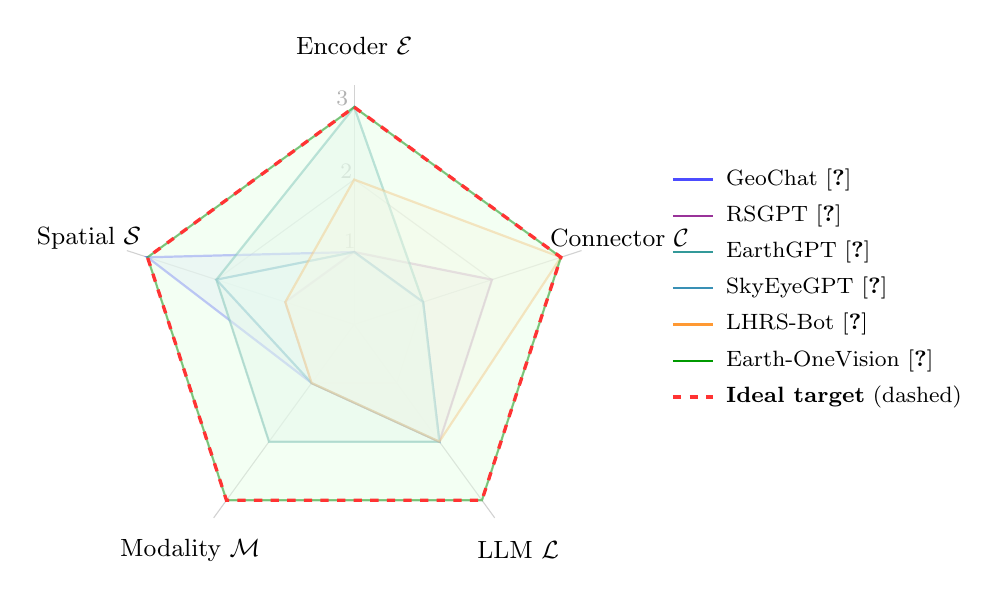
\begin{tikzpicture}[scale=0.92]
  %% ── Radar axes (5 axes, starting top, 72 deg apart) ──────
  \foreach \ang/\lbl in {
      90/{Encoder $\mathcal{E}$},
      18/{Connector $\mathcal{C}$},
      -54/{LLM $\mathcal{L}$},
      -126/{Modality $\mathcal{M}$},
      162/{Spatial $\mathcal{S}$}}{
    \draw[gray!35, thin] (0,0) -- (\ang:3.3cm);
    \node[font=\small] at (\ang:3.85cm) {\lbl};
  }
  %% ── Grid rings at r = 1, 2, 3 ───────────────────────────
  \foreach \r in {1,2,3}{
    \draw[gray!30, thin]
      (90:\r cm)--(18:\r cm)--(-54:\r cm)--(-126:\r cm)--(162:\r cm)--cycle;
  }
  %% ── Axis tick labels ─────────────────────────────────────
  \node[gray!60, font=\footnotesize] at (93:1.15cm) {1};
  \node[gray!60, font=\footnotesize] at (93:2.12cm) {2};
  \node[gray!60, font=\footnotesize] at (93:3.12cm) {3};

  %% ── Model polygons ───────────────────────────────────────
  %% GeoChat  [1]: E=1,C=1,L=2,M=1,S=3
  \draw[blue!70,   thick, fill=blue!10,   opacity=0.55]
    (90:1cm)--(18:1cm)--(-54:2cm)--(-126:1cm)--(162:3cm)--cycle;
  %% RSGPT    [2]: E=1,C=2,L=2,M=1,S=1
  \draw[violet!80, thick, fill=violet!10, opacity=0.45]
    (90:1cm)--(18:2cm)--(-54:2cm)--(-126:1cm)--(162:1cm)--cycle;
  %% EarthGPT [3]: E=3,C=1,L=2,M=2,S=2
  \draw[teal!80,   thick, fill=teal!10,   opacity=0.50]
    (90:3cm)--(18:1cm)--(-54:2cm)--(-126:2cm)--(162:2cm)--cycle;
  %% SkyEyeGPT [4]: E=1,C=1,L=2,M=1,S=2
  \draw[cyan!70!black, thick, fill=cyan!8, opacity=0.45]
    (90:1cm)--(18:1cm)--(-54:2cm)--(-126:1cm)--(162:2cm)--cycle;
  %% LHRS-Bot [5]: E=2,C=3,L=2,M=1,S=1
  \draw[orange!80,  thick, fill=orange!10, opacity=0.45]
    (90:2cm)--(18:3cm)--(-54:2cm)--(-126:1cm)--(162:1cm)--cycle;
  %% Earth-OneVision [6]: E=3,C=3,L=3,M=3,S=3
  \draw[green!60!black, thick, fill=green!10, opacity=0.45]
    (90:3cm)--(18:3cm)--(-54:3cm)--(-126:3cm)--(162:3cm)--cycle;
  %% Ideal (dashed red)
  \draw[red!80, very thick, dashed]
    (90:3cm)--(18:3cm)--(-54:3cm)--(-126:3cm)--(162:3cm)--cycle;

  %% ── Legend ───────────────────────────────────────────────
  \begin{scope}[xshift=4.4cm, yshift=0.5cm, font=\footnotesize]
    \draw[blue!70,        thick] (0,1.5)--(0.55,1.5);
    \node[anchor=west] at (0.60,1.5) {GeoChat~\cite{geochat2024}};
    \draw[violet!80,      thick] (0,1.0)--(0.55,1.0);
    \node[anchor=west] at (0.60,1.0) {RSGPT~\cite{rsgpt2023}};
    \draw[teal!80,        thick] (0,0.5)--(0.55,0.5);
    \node[anchor=west] at (0.60,0.5) {EarthGPT~\cite{earthgpt2025}};
    \draw[cyan!70!black,  thick] (0,0.0)--(0.55,0.0);
    \node[anchor=west] at (0.60,0.0) {SkyEyeGPT~\cite{skyeyegpt2025}};
    \draw[orange!80,      thick] (0,-0.5)--(0.55,-0.5);
    \node[anchor=west] at (0.60,-0.5) {LHRS-Bot~\cite{lhrsbot2024}};
    \draw[green!60!black, thick] (0,-1.0)--(0.55,-1.0);
    \node[anchor=west] at (0.60,-1.0) {Earth-OneVision~\cite{earthonevision2026}};
    \draw[red!80, very thick, dashed] (0,-1.5)--(0.55,-1.5);
    \node[anchor=west] at (0.60,-1.5) {\textbf{Ideal target} (dashed)};
  \end{scope}
\end{tikzpicture}
\caption{Five-dimensional design-space radar chart for six representative RS-MLLMs
and the target ideal model (heavy dashed line, labelled ``Ideal'' in legend).
Axis scale: 1\,=\,minimal / absent, 3\,=\,most sophisticated / complete.
No existing model reaches the ideal polygon.
The largest deficits appear on the Modality\,($\mathcal{M}$) and Spatial
Output\,($\mathcal{S}$) axes, the dimensions most critical for real-world
geospatial intelligence.}\label{fig:radar_5d}
\end{figure}

The following five subsections analyse each dimension in detail.

%% ──────────────────────────────────────────────────────────────
\subsection{Dimension \texorpdfstring{$\mathcal{E}$}{E}: Vision Encoder Adaptation}\label{sec3:encoder}
%% ──────────────────────────────────────────────────────────────

The vision encoder is the first component an RS image passes through. General-purpose
MLLMs rely on CLIP ViT-L/14 or EVA-CLIP~\cite{fang2023evaclip} pre-trained on billions of internet
image--text pairs. However, RS images differ fundamentally from internet photographs: they
are acquired from a nadir (top-down) viewpoint, exhibit spectral diversity across sensor
types, and present scale variation spanning several orders of magnitude. These properties
create a \emph{domain gap} that CLIP encoders were never trained to bridge, and which
propagates through all downstream RS tasks. We identify four encoder adaptation strategies
in the RS-MLLM literature, illustrated in Fig.~\ref{fig:encoder_spectrum}.

\textbf{Type~A: CLIP-Inherited.}
The simplest approach reuses a frozen or lightly fine-tuned CLIP encoder without any
RS-specific modification. GeoChat~\cite{geochat2024} uses CLIP-ViT-L/14; RSGPT~\cite{rsgpt2023}
uses EVA-CLIP-G~\cite{fang2023evaclip}; RS-LLaVA~\cite{rsllava2024} adopts the same strategy. Integration with
established MLLM pipelines is straightforward, but the encoder inherits CLIP's
\emph{blind-pair} failure mode: two semantically distinct RS images---such as a dense
urban tile and a sparse rural tile---can receive near-identical CLIP embeddings
because CLIP has no RS training signal~\cite{bommasani2021}.

\textbf{Type~B: RS-Pretrained CLIP.}
A second approach replaces the general CLIP encoder with a variant pre-trained on RS
image--text pairs. RemoteCLIP~\cite{remoteclip2024} contrastively trains on RSICD, UCM,
and PatternNet. GeoRSCLIP~\cite{georscclip2024} and its large-scale RS5M training corpus~\cite{lin2024rs5m}, as well as SkyCLIP~\cite{skyclip2024} follow
analogous strategies with different RS corpora. These encoders partially close the
optical RS domain gap but do not address SAR or hyperspectral modalities, which lack
the large-scale image--text pair data required for contrastive pre-training.

\textbf{Type~C: Hybrid CNN + ViT.}
EarthGPT~\cite{earthgpt2025} combines a DINOv2~\cite{oquab2023dinov2} ViT for global semantic features with a
parallel CNN pathway for local texture and spatial detail. The two streams are fused
before the connector, providing multi-granular representations. This design is motivated
by the complementary strengths of ViTs (long-range context) and CNNs (high-frequency
spatial detail), both critical for RS small-object detection. The trade-off is a
substantially increased encoder memory footprint.

\textbf{Type~D: Multi-Depth ViT Injection.}
Earth-OneVision~\cite{earthonevision2026} extracts intermediate feature maps from
multiple ViT layers---not only the final output token---and injects them into the
connector via an \emph{Adaptive Cross-layer Self-Attention} (ACSA) module. This
preserves both low-level spatial detail from early ViT layers and high-level semantic
context from late layers, directly addressing the extreme scale-variation challenge
characteristic of RS imagery. The cost is higher GPU memory and inference latency
compared to Types~A--C.

\begin{figure}[h]
\centering
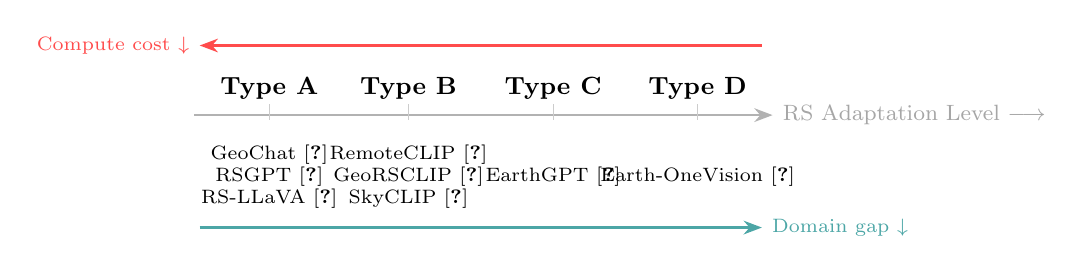
\begin{tikzpicture}[font=\small, >=Stealth, scale=0.68]
  %% Main spectrum arrow
  \draw[->, thick, gray!60] (-0.2,0) -- (10.6,0)
    node[right, gray!70, font=\footnotesize] {RS Adaptation Level $\longrightarrow$};
  %% Type labels and model annotations
  %% Type A
  \node[font=\bfseries\small] at (1.2, 0.5) {Type~A};
  \draw[gray!40] (1.2,0.2)--(1.2,-0.1);
  \node[align=center,font=\scriptsize] at (1.2,-1.15)
    {GeoChat~\cite{geochat2024}\\RSGPT~\cite{rsgpt2023}\\RS-LLaVA~\cite{rsllava2024}};
  %% Type B
  \node[font=\bfseries\small] at (3.8, 0.5) {Type~B};
  \draw[gray!40] (3.8,0.2)--(3.8,-0.1);
  \node[align=center,font=\scriptsize] at (3.8,-1.15)
    {RemoteCLIP~\cite{remoteclip2024}\\GeoRSCLIP~\cite{georscclip2024}\\SkyCLIP~\cite{skyclip2024}};
  %% Type C
  \node[font=\bfseries\small] at (6.5, 0.5) {Type~C};
  \draw[gray!40] (6.5,0.2)--(6.5,-0.1);
  \node[align=center,font=\scriptsize] at (6.5,-1.15) {EarthGPT~\cite{earthgpt2025}};
  %% Type D
  \node[font=\bfseries\small] at (9.2, 0.5) {Type~D};
  \draw[gray!40] (9.2,0.2)--(9.2,-0.1);
  \node[align=center,font=\scriptsize] at (9.2,-1.15) {Earth-OneVision~\cite{earthonevision2026}};
  %% Domain gap arrow (bottom, left to right = gap decreases)
  \draw[->, teal!70, thick] (-0.1,-2.1) -- (10.4,-2.1)
    node[right, teal!70, font=\scriptsize] {Domain gap $\downarrow$};
  %% Compute cost arrow (top, right to left = cost decreases going left)
  \draw[->, red!70, thick] (10.4,1.3) -- (-0.1,1.3)
    node[left, red!70, font=\scriptsize] {Compute cost $\downarrow$};
\end{tikzpicture}
\caption{Encoder adaptation spectrum for RS-MLLMs (Types A--D). Moving from Type~A to
Type~D progressively reduces the RS domain gap (teal arrow, bottom) at the cost of
increasing computational complexity (red arrow, top). Type~A models inherit CLIP's
blind-pair limitation and are the predominant choice ($\approx$77\,\% of surveyed
models); Type~D achieves the richest RS feature representations.}\label{fig:encoder_spectrum}
\end{figure}

%% ──────────────────────────────────────────────────────────────
\subsection{Dimension \texorpdfstring{$\mathcal{C}$}{C}: Vision-Language Connector}\label{sec3:connector}
%% ──────────────────────────────────────────────────────────────

The vision-language connector maps visual feature tokens into the LLM embedding space.
For natural images ($224\!\times\!224$ to $512\!\times\!512$ pixels), a linear MLP
projection is typically sufficient. RS imagery routinely reaches
$1024\!\times\!1024$ to $8192\!\times\!8192$ pixels, producing token sequences that
far exceed standard LLM context windows. The connector must therefore balance
\emph{information retention} against \emph{token budget}---a trade-off that general
MLLM connectors are not designed to optimise. We identify five connector types in the
RS-MLLM literature, visualised in Fig.~\ref{fig:connector_types}.

\textbf{Type~A: Linear MLP Projection.}
A two-layer MLP maps visual tokens to the LLM embedding dimension. SkyEyeGPT~\cite{skyeyegpt2025}
and RS-LLaVA~\cite{rsllava2024} both adopt this design. It is computationally inexpensive
and easy to train, but produces no token compression, causing context-window saturation
at RS resolutions above approximately $1024\!\times\!1024$ pixels. Despite this
limitation, the MLP connector is the most frequently used design (17\,/\,26 models),
reflecting the prevalence of moderate-resolution optical RS benchmarks in the training data.

\textbf{Type~B: Instruction-Aware Q-Former.}
RSGPT~\cite{rsgpt2023} adapts the InstructBLIP Q-Former~\cite{instructblip2023} for RS.
Learnable query tokens cross-attend to visual features conditioned on the language
instruction, producing a fixed-length output sequence irrespective of input resolution.
The instruction conditioning allows selective attention to task-relevant image regions,
which benefits targeted VQA, but the fixed query budget can discard spatial detail
needed for oriented object detection.

\textbf{Type~C: Perceiver Resampler.}
LHRS-Bot~\cite{lhrsbot2024} and LHRS-Bot-Nova~\cite{lhrsbotnova2024} employ a Perceiver
Resampler that maps variable-length visual sequences to a fixed-length output via
cross-attention. Unlike the Q-Former, the resampler is not instruction-conditioned,
preserving a spatially uniform representation that is better suited to dense RS tasks
such as scene classification and image captioning.

\textbf{Type~D: Multi-Scale Cross-Attention.}
Earth-OneVision~\cite{earthonevision2026} introduces an ACSA connector that aggregates
feature maps from multiple ViT layers via cross-attention, followed by a DeepStack module
that interleaves visual tokens across LLM depth. This enables the LLM to access both
coarse semantic and fine spatial features at different processing stages, directly
addressing RS scale variation.

\textbf{Type~E: Budget-Aware Token Compression.}
GeoLLaVA-8K~\cite{geollava2025} and UHR-BAT~\cite{uhrbat2025} target ultra-high-resolution
RS imagery ($4096$--$8192$ pixels) through token compression. GeoLLaVA-8K applies
coarse-to-fine tiling with a token budget ceiling; UHR-BAT uses a learned pruning
mechanism that retains high-saliency tokens while discarding background tokens. These
are the only connector designs that make RS-MLLM inference feasible at extreme
RS resolutions.

\begin{figure}[h]
\centering
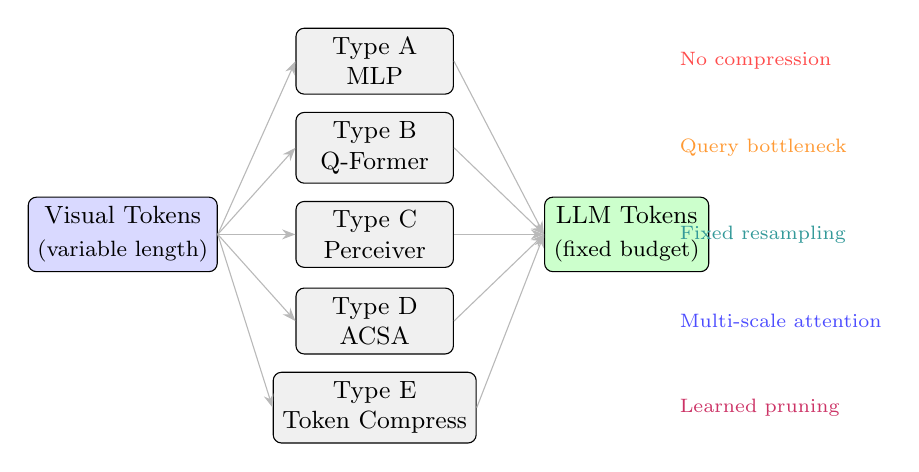
\begin{tikzpicture}[font=\small, >=Stealth,
    box/.style={draw, rounded corners=3pt, fill=#1, minimum width=2.0cm,
                minimum height=0.60cm, align=center}]
  %% Input
  \node[box=blue!15]   (inp) at (0,0)
    {Visual Tokens\\[1pt]{\footnotesize (variable length)}};
  %% Five connectors
  \node[box=gray!12] (ta) at (3.2, 2.2) {Type~A\\MLP};
  \node[box=gray!12] (tb) at (3.2, 1.1) {Type~B\\Q-Former};
  \node[box=gray!12] (tc) at (3.2, 0.0) {Type~C\\Perceiver};
  \node[box=gray!12] (td) at (3.2,-1.1) {Type~D\\ACSA};
  \node[box=gray!12] (te) at (3.2,-2.2) {Type~E\\Token Compress};
  %% Output
  \node[box=green!20] (out) at (6.4,0)
    {LLM Tokens\\[1pt]{\footnotesize (fixed budget)}};
  %% Arrows
  \foreach \n in {ta,tb,tc,td,te}{
    \draw[->,gray!55] (inp.east) -- (\n.west);
    \draw[->,gray!55] (\n.east) -- (out.west);
  }
  %% Annotations
  \node[red!70,    right, font=\scriptsize] at (6.95, 2.2) {No compression};
  \node[orange!80, right, font=\scriptsize] at (6.95, 1.1) {Query bottleneck};
  \node[teal!80,   right, font=\scriptsize] at (6.95, 0.0) {Fixed resampling};
  \node[blue!70,   right, font=\scriptsize] at (6.95,-1.1) {Multi-scale attention};
  \node[purple!80, right, font=\scriptsize] at (6.95,-2.2) {Learned pruning};
\end{tikzpicture}
\caption{Five vision-language connector types identified in RS-MLLM literature.
All connectors map variable-length visual token sequences to a fixed LLM token
budget; they differ in information retention and compression strategy. Only
Type~E connectors are suitable for ultra-high-resolution RS imagery
($\geq\!4096$ pixels), yet remain in use by fewer than two
models.}\label{fig:connector_types}
\end{figure}

%% ──────────────────────────────────────────────────────────────
\subsection{Dimension \texorpdfstring{$\mathcal{L}$}{L}: LLM Backbone and Freezing Strategy}\label{sec3:llm}
%% ──────────────────────────────────────────────────────────────

The LLM backbone provides language understanding, instruction following, and response
generation. RS researchers face a severe compute trade-off: large LLMs
($\geq\!13$\,B parameters) offer stronger reasoning but are prohibitively expensive to
fine-tune for most academic groups. Three freezing strategies have emerged, reflecting
different points on this trade-off.

\textit{Full freeze with LoRA adaptation} is the dominant approach.
All LLM parameters are frozen and Low-Rank Adaptation (LoRA)~\cite{hu2022lora} modules
are inserted into the attention layers. GeoChat~\cite{geochat2024},
RSGPT~\cite{rsgpt2023}, SkyEyeGPT~\cite{skyeyegpt2025}, LHRS-Bot~\cite{lhrsbot2024},
and VHM~\cite{vhm2025} all adopt this strategy. LoRA with rank $r \in [16,\,64]$ is
sufficient for RS VQA and captioning while reducing trainable parameters by more than
95\,\%, making training feasible on 2--4 NVIDIA A100 GPUs---the typical hardware budget
of RS academic groups. The full-freeze strategy accounts for 19 of the 26 models in our
taxonomy.

\textit{Partial unfreeze} is employed by EarthGPT~\cite{earthgpt2025}, which allows
gradient updates to flow into self-attention layers and RMSNorm parameters while keeping
feed-forward layers frozen. This \emph{bias-tuning} variant increases trainable
parameters to approximately 8\,\% of the total but enables more flexible adaptation to
the multi-sensor instruction distribution of MMRS-1M.

\textit{Full fine-tuning} is rare due to compute cost.
Earth-OneVision~\cite{earthonevision2026} is the only published RS-MLLM to train with a
full supervised fine-tuning pipeline, requiring 34\,M instruction pairs across six sensor
modalities. No published RS-MLLM has adopted a backbone exceeding 13\,B parameters,
reflecting the compute constraints of the RS research community.

Backbone choices across the literature include Vicuna-7B\,/\,13B~\cite{vicuna2023},
LLaMA-2-7B\,/\,13B~\cite{llama2023}, InternLM-7B~\cite{internlm2023}, and
Qwen-7B~\cite{qwen2023}.

%% ──────────────────────────────────────────────────────────────
\subsection{Dimension \texorpdfstring{$\mathcal{M}$}{M}: Sensor Modality Scope}\label{sec3:modality}
%% ──────────────────────────────────────────────────────────────

Remote sensing is inherently multi-modal: optical sensors measure solar reflectance,
SAR sensors measure radar backscatter, and hyperspectral sensors resolve hundreds of
narrow spectral bands. A geospatially intelligent RS-MLLM must ultimately reason across
all modalities. We classify existing models into four modality scope levels.

\textit{Level~1 (Optical-only)} covers more than 85\,\% of all published RS-MLLMs,
including GeoChat~\cite{geochat2024}, SkyEyeGPT~\cite{skyeyegpt2025},
RSGPT~\cite{rsgpt2023}, LHRS-Bot~\cite{lhrsbot2024}, H2RSVLM~\cite{h2rsvlm2025},
RS-LLaVA~\cite{rsllava2024}, VHM~\cite{vhm2025}, and more than 20 additional models.
The observed dominance of optical imagery is consistent with CLIP pre-training:
CLIP was trained on
internet photographs, which are almost exclusively optical RGB, providing a useful visual
prior for optical RS imagery that does not exist for SAR or HSI.

\textit{Level~2 (Optical\,+\,SAR)} is achieved by EarthGPT~\cite{earthgpt2025}, the
first RS-MLLM to jointly process optical, SAR, and infrared imagery within a unified
model trained on MMRS-1M (one million image--text pairs across three sensor types).
SARChat-Bench-2M~\cite{sarchatchat2025} provides two million SAR dialogue pairs for
fine-tuning, but joint optical--SAR training in a single model remains uncommon.

\textit{Level~3 (Multi-sensor unified)} is achieved by Earth-OneVision~\cite{earthonevision2026},
which processes six sensor modalities (optical, SAR, infrared, multispectral,
temporal, and video) within a single model architecture, covering nine task categories.
Earth-OneVision represents the most comprehensive modality scope of any published
RS-MLLM and substantially narrows the multi-sensor gap. However, it uses a
unified optical-domain encoder for all modalities without physics-informed
specialisation, and provides no HSI support---leaving Level~4 (HSI-aware)
entirely unfilled.

\textit{Level~4 (HSI-aware)} is an unfilled gap. No dedicated hyperspectral RS-MLLM
exists as of mid-2026. HM-Bench~\cite{hmbench2026} provides the first evaluation
framework for HSI-specific MLLM tasks (19,337 expert-annotated samples across 13 task
categories) and evaluates 18 general-purpose MLLMs on spectral reasoning tasks. All 18
models show significant difficulty, confirming that the Level-4 modality gap is both
real and structurally unaddressed~\cite{hmbench2026}. We return to this finding in the
hallucination analysis of Sect.~\ref{sec7}.

Figure~\ref{fig:modality_heatmap} visualises modality coverage across 12 representative
RS-MLLMs chronologically. The dominance of optical modality is structurally apparent:
the SAR and HSI columns are empty for all models prior to 2025 and only partially
filled thereafter.

\begin{figure}[h]
\centering
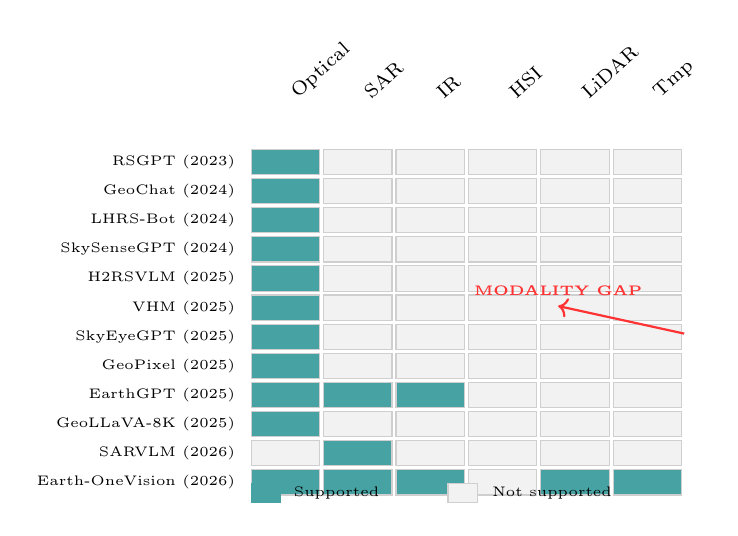
\begin{tikzpicture}[font=\scriptsize]
  %% Column headers (rotated 40 degrees)
  \foreach \j/\lbl in {0/Optical,1/SAR,2/IR,3/HSI,4/LiDAR,5/Tmp/Vid}{
    \node[rotate=42, anchor=west] at ({0.92*\j+0.46}, 4.55) {\lbl};
  }
  %% Row data: {i}/{label}/{o,s,i,h,l,m}
  \foreach \i/\mname/\oa/\sa/\ira/\hs/\li/\mt in {
    0/{RSGPT (2023)}/1/0/0/0/0/0,
    1/{GeoChat (2024)}/1/0/0/0/0/0,
    2/{LHRS-Bot (2024)}/1/0/0/0/0/0,
    3/{SkySenseGPT (2024)}/1/0/0/0/0/0,
    4/{H2RSVLM (2025)}/1/0/0/0/0/0,
    5/{VHM (2025)}/1/0/0/0/0/0,
    6/{SkyEyeGPT (2025)}/1/0/0/0/0/0,
    7/{GeoPixel (2025)}/1/0/0/0/0/0,
    8/{EarthGPT (2025)}/1/1/1/0/0/0,
    9/{GeoLLaVA-8K (2025)}/1/0/0/0/0/0,
   10/{SARVLM (2026)}/0/1/0/0/0/0,
   11/{Earth-OneVision (2026)}/1/1/1/0/1/1}{
    %% Row label
    \node[anchor=east, font=\tiny] at (-0.08, {3.78-\i*0.37}) {\mname};
    %% Cells
    \foreach \j/\val in {0/\oa,1/\sa,2/\ira,3/\hs,4/\li,5/\mt}{
      \ifnum\val=1
        \fill[teal!72] ({0.92*\j}, {3.62-\i*0.37}) rectangle ++(0.87,0.32);
      \else
        \fill[gray!10] ({0.92*\j}, {3.62-\i*0.37}) rectangle ++(0.87,0.32);
      \fi
      \draw[gray!38] ({0.92*\j}, {3.62-\i*0.37}) rectangle ++(0.87,0.32);
    }
  }
  %% Legend
  \fill[teal!72]  (0.0,-0.55) rectangle ++(0.38,0.25);
  \node[right, font=\tiny] at (0.42,-0.42) {Supported};
  \fill[gray!10]  (2.5,-0.55) rectangle ++(0.38,0.25);
  \draw[gray!38]  (2.5,-0.55) rectangle ++(0.38,0.25);
  \node[right, font=\tiny] at (2.94,-0.42) {Not supported};
  %% GAP annotation
  \draw[red!80, thick, ->] (5.5,1.60) -- (3.90,1.95)
    node[above, font=\tiny\bfseries, red!80] {MODALITY GAP};
\end{tikzpicture}
\caption{Sensor modality coverage heatmap for 12 representative RS-MLLMs
(2023--2026). Optical modality dominates across all years. SAR and infrared
support is limited to EarthGPT~\cite{earthgpt2025} and
Earth-OneVision~\cite{earthonevision2026}. Earth-OneVision also supports
temporal and video modalities (Tmp/Vid column). HSI support is absent in
all published RS-MLLMs; HM-Bench~\cite{hmbench2026} provides evaluation
infrastructure but no dedicated HSI RS-MLLM
exists.}\label{fig:modality_heatmap}
\end{figure}

%% ──────────────────────────────────────────────────────────────
\subsection{Dimension \texorpdfstring{$\mathcal{S}$}{S}: Spatial Output Capability}\label{sec3:spatial}
%% ──────────────────────────────────────────────────────────────

The spatial output capability of an RS-MLLM determines which detection and localisation
tasks it can perform. This dimension is motivated by a distinctive RS challenge:
aircraft, ships, and vehicles appear at arbitrary rotation angles in nadir-view imagery,
making horizontal bounding boxes (HBB) a poor fit. An HBB enclosing a rotated aircraft
wastes 55--70\,\% of its area on background pixels~\cite{xia2018dota}. Oriented
bounding boxes (OBB), parameterised as $(x, y, w, h, \theta)$, eliminate this waste but
require a model capable of outputting angular coordinates---a capability absent from all
general MLLM baselines. We organise spatial output capability into five levels,
illustrated in Fig.~\ref{fig:spatial_ladder}.

\textit{Level~1 (Text-only):} RSGPT~\cite{rsgpt2023}, RS-LLaVA~\cite{rsllava2024},
LHRS-Bot~\cite{lhrsbot2024}, and VHM~\cite{vhm2025} produce text responses only. Spatial
queries are answered descriptively rather than as coordinate outputs, limiting these
models to VQA and captioning tasks.

\textit{Level~2 (HBB coordinates):} EarthGPT~\cite{earthgpt2025},
SkyEyeGPT~\cite{skyeyegpt2025}, and TEOChat~\cite{teochat2025} generate HBB coordinates
as structured text tokens (\texttt{[x1,\;y1,\;x2,\;y2]}). This enables visual grounding
and language-conditioned detection, but remains suboptimal for rotated RS objects due to
the area-waste problem described above.

\textit{Level~3 (OBB coordinates):} OBB output is present in four Corpus~B
models: GeoChat~\cite{geochat2024}, EarthGPT~\cite{earthgpt2025},
GeoGround~\cite{geoground2025}, and EarthGPT-X~\cite{earthgptx2026}.
However, these differ substantially in OBB scope. GeoChat produces
conversational OBB across arbitrary RS queries, as confirmed by two
independent sources: the GeoGround paper~\cite{geoground2025} states
``GeoChat outputs rotated bounding boxes'' and the GeoPixel
paper~\cite{geopixel2025} states ``for GeoChat, we convert its output
OBBs to HBBs'' during evaluation.
EarthGPT produces HBB+OBB in zero-shot detection mode only;
GeoGround produces OBB in visual-grounding (single-referent) mode only;
EarthGPT-X extends EarthGPT with HSI+SAR inputs but retains the
task-constrained OBB scope.
The real Level~3 gap is therefore not the absence of any OBB model,
but two more specific deficits: (i)~\emph{generality}---4/26 Corpus~B
models provide \emph{any} OBB capability, but only 1/26 (GeoChat)
produces general-purpose conversational OBB across arbitrary query
types; and (ii)~\emph{cross-sensor OBB}---all four models are
confined to optical DOTA imagery~\cite{xia2018dota} and no model
produces SAR or HSI OBB output. OBB performance across all four
models remains far below specialist detectors such as Oriented
R-CNN~\cite{xie2021orientedrcnn}.

\textit{Level~4 (Segmentation mask):} GeoPixel~\cite{geopixel2025},
GeoPix~\cite{geopix2025}, and SegEarth-R1~\cite{segearth2026} produce pixel-level
segmentation masks. GeoPixel introduces a pixel grounding task for RS imagery and
demonstrates that MLLMs can generate spatially precise masks when fine-tuned with
pixel-level RS annotations.

\textit{Level~5 (Cross-sensor OBB\,+\,Segmentation---GAP):} No published RS-MLLM
supports OBB detection across multiple sensor modalities or combines pixel-level
segmentation with cross-sensor OBB. This Level-5 capability is critical for operational
applications such as maritime vessel monitoring (SAR\,+\,optical) and precision
agriculture (multispectral\,+\,HSI), and represents the most significant structural gap
in current RS-MLLM spatial output design.

\begin{figure}[h]
\centering
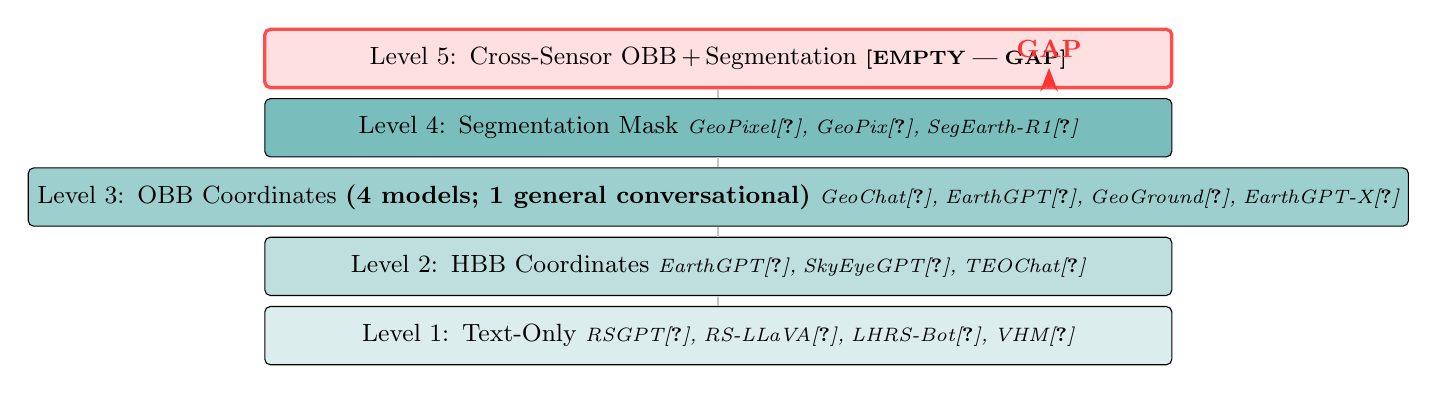
\begin{tikzpicture}[font=\small, >=Stealth,
    rung/.style={draw, fill=#1, minimum width=0.95\textwidth,
                 minimum height=0.74cm, align=center, rounded corners=2pt}]
  \node[rung=teal!14] (l1) at (0,0.00)
    {Level~1:\enskip Text-Only
     \hfill {\itshape\scriptsize RSGPT\cite{rsgpt2023},\;RS-LLaVA\cite{rsllava2024},\;LHRS-Bot\cite{lhrsbot2024},\;VHM\cite{vhm2025}}};
  \node[rung=teal!25] (l2) at (0,0.88)
    {Level~2:\enskip HBB Coordinates
     \hfill {\itshape\scriptsize EarthGPT\cite{earthgpt2025},\;SkyEyeGPT\cite{skyeyegpt2025},\;TEOChat\cite{teochat2025}}};
  \node[rung=teal!38] (l3) at (0,1.76)
    {Level~3:\enskip OBB Coordinates \textbf{(4 models; 1 general conversational)}
     \hfill {\itshape\scriptsize GeoChat\cite{geochat2024},\;EarthGPT\cite{earthgpt2025},\;GeoGround\cite{geoground2025},\;EarthGPT-X\cite{earthgptx2026}}};
  \node[rung=teal!52] (l4) at (0,2.64)
    {Level~4:\enskip Segmentation Mask
     \hfill {\itshape\scriptsize GeoPixel\cite{geopixel2025},\;GeoPix\cite{geopix2025},\;SegEarth-R1\cite{segearth2026}}};
  \node[rung=red!12, draw=red!70, very thick] (l5) at (0,3.52)
    {Level~5:\enskip Cross-Sensor OBB\,+\,Segmentation
     \hfill {\bfseries\scriptsize [EMPTY\;---\;GAP]}};
  %% Connecting bars between rungs
  \foreach \from/\to in {l1/l2,l2/l3,l3/l4,l4/l5}
    \draw[thick, gray!45] (\from.north) -- (\to.south);
  %% GAP annotation
  \draw[red!80, very thick, ->] (4.2, 3.16) -- (4.2, 3.40)
    node[above, font=\bfseries\small, red!80] {GAP};
\end{tikzpicture}
\caption{Spatial output capability ladder for RS-MLLMs. Level~3 (OBB) is
occupied by four Corpus~B models, but with substantially different scopes.
\textbf{General conversational OBB} (1/26): GeoChat~\cite{geochat2024} produces OBB
across arbitrary RS queries.
\textbf{Task-constrained OBB} (3/26): EarthGPT~\cite{earthgpt2025} (zero-shot
detection mode only), GeoGround~\cite{geoground2025} (single-referent
visual-grounding mode only), and EarthGPT-X~\cite{earthgptx2026}
(task-constrained OBB with HSI+SAR input).
All four are confined to optical DOTA imagery~\cite{xia2018dota};
no model extends OBB output to SAR or HSI sensor modalities.
Level~5 (cross-sensor OBB\,+\,segmentation) is entirely
unoccupied---this, rather than the total absence of OBB, is the
primary structural gap for real-world RS detection
applications.}\label{fig:spatial_ladder}
\end{figure}

%% ──────────────────────────────────────────────────────────────
\subsection{Master RS-MLLM Architecture Comparison}\label{sec3:master}
%% ──────────────────────────────────────────────────────────────

Table~\ref{tab:master_comparison} presents the RS-MLLM architecture registry
(Corpus~B: 26 distinct RS-MLLMs) across all five design-space dimensions.
The 26 architectures arise from 31 model-related publications;
5 are companion or extension reports of already-registered architectures.
The final row presents the \emph{ideal} RS-MLLM---a model achieving the highest capability
on every dimension---which no existing system realises.

\begin{sidewaystable}
\tiny\setlength\tabcolsep{2pt}\renewcommand{\arraystretch}{1.05}
\caption{Master RS-MLLM architecture comparison across the five design-space
dimensions~(\ref{eq:design_space}). \textbf{Enc.:} A\,=\,CLIP-inherited,
B\,=\,RS-pretrained CLIP, C\,=\,CNN+ViT hybrid, D\,=\,Multi-depth ViT.
\textbf{Conn.:} MLP, QF\,=\,Q-Former, PR\,=\,Perceiver, ACSA\,=\,multi-scale cross-attn,
TC\,=\,token compression, PD\,=\,pixel decoder.
\textbf{Mod.:} Opt\,=\,Optical, IR\,=\,Infrared, HSI\,=\,Hyperspectral.
\textbf{Out.:} T\,=\,Text, HBB, OBB, Seg\,=\,Segmentation.
\textbf{Tr.:} FZ\,=\,Full freeze+LoRA, PU\,=\,Partial unfreeze, FF\,=\,Full SFT.
\textbf{Open:} \checkmark\,=\,weights released.
$\dagger$~Ideal: design target; no existing model achieves all cells.}\label{tab:master_comparison}
\begin{tabular*}{\textheight}{@{\extracolsep\fill}p{1.85cm}lp{0.95cm}llp{1.45cm}p{1.55cm}p{1.15cm}lcp{1.4cm}cp{1.75cm}}
\toprule
\textbf{Model} & \textbf{Yr} & \textbf{Venue} &
\textbf{Enc.} & \textbf{Conn.} & \textbf{LLM Backbone} &
\textbf{Modality} & \textbf{Output} & \textbf{Tr.} &
\textbf{Param} & \textbf{Wt} & \textbf{Inst.\,Data} &
\textbf{Benchmark} \\
\midrule
RSGPT~\cite{rsgpt2023}                    & 23 & arXiv    & A & QF   & Vicuna-7B    & Opt           & T        & FZ  & 7B   & --         & RSICap\,(2K)      & RSICap, RSVQA \\
GeoChat~\cite{geochat2024}                & 24 & CVPR     & A & MLP  & Vicuna-7B    & Opt           & OBB      & FZ  & 7B   & \checkmark & GCI\,(318K)       & GeoChat-Bench \\
SkySenseGPT~\cite{skysensegpt2024}        & 24 & arXiv    & A & MLP  & LLaMA-2-7B   & Opt           & T        & FZ  & 7B   & --         & RS-Inst\,(1M)     & GeoChat-Bench \\
LHRS-Bot~\cite{lhrsbot2024}               & 24 & arXiv    & B & PR   & LLaMA-2-13B  & Opt           & T        & FZ  & 13B  & \checkmark & LHRS\,(1.15M)     & RSVQA, RSICD \\
LHRS-Bot-Nova~\cite{lhrsbotnova2024}      & 24 & arXiv    & B & PR   & LLaMA-2-13B  & Opt           & T        & FZ  & 13B  & \checkmark & LHRS-v2           & RSVQA, RSICD \\
RS-LLaVA~\cite{rsllava2024}               & 24 & MDPI RS  & A & MLP  & LLaMA-2-7B   & Opt           & T        & FZ  & 7B   & \checkmark & RSVQA\,(77K)      & RSVQA, RSICD \\
VRSBench~\cite{vrsbench2024}              & 24 & arXiv    & A & MLP  & LLaMA-2-7B   & Opt           & T+HBB    & FZ  & 7B   & \checkmark & VRSBench\,(1M)    & VRSBench \\
Change-Agent~\cite{changeagent2025}       & 25 & arXiv    & A & MLP  & InternLM-7B  & Opt           & T        & FZ  & 7B   & \checkmark & LEVIR-CD          & LEVIR-CD \\
H2RSVLM~\cite{h2rsvlm2025}               & 25 & AAAI     & A & MLP  & InternLM-7B  & Opt           & HBB      & FZ  & 7B   & \checkmark & H2RSVLM-B         & H2RSVLM-Bench \\
VHM~\cite{vhm2025}                        & 25 & AAAI     & A & MLP  & InternLM-7B  & Opt           & T+HBB    & FZ  & 7B   & \checkmark & VHM-B\,(NR)       & VHM-Bench \\
SkyEyeGPT~\cite{skyeyegpt2025}            & 25 & ISPRS JP & A & MLP  & InternLM-7B  & Opt           & HBB+T    & FZ  & 7B   & \checkmark & SkyEye\,(968K)    & SkyEye-968K \\
EarthGPT~\cite{earthgpt2025}              & 25 & TGRS     & C & MLP  & InternLM-7B  & Opt+SAR+IR    & HBB+OBB  & PU  & 7B   & --         & MMRS-1M           & MMRS-1M \\
GeoLLaVA-8K~\cite{geollava2025}           & 25 & arXiv    & A & TC   & LLaMA-2-7B   & Opt           & T+HBB    & FZ  & 7B   & --         & GeoLLaVA\,(NR)    & XLRS-Bench \\
TEOChat~\cite{teochat2025}                & 25 & arXiv    & A & MLP  & LLaMA-2-7B   & Opt           & HBB+T    & FZ  & 7B   & \checkmark & TEO-Instruct      & LEVIR-CD \\
GeoGround~\cite{geoground2025}            & 25 & arXiv    & A & MLP  & InternLM-7B  & Opt           & HBB+OBB  & FZ  & 7B   & \checkmark & RSVG\,(38K)       & RSVG \\
UHR-BAT~\cite{uhrbat2025}                 & 25 & arXiv    & A & TC   & LLaMA-2-7B   & Opt           & T+HBB    & FZ  & 7B   & --         & XLRS-B\,(12K)     & XLRS-Bench \\
GeoPixel~\cite{geopixel2025}              & 25 & arXiv    & A & PD   & InternLM-7B  & Opt           & Seg      & FZ  & 7B   & \checkmark & GeoPixel-Inst     & GeoPixel-Inst \\
GeoPix~\cite{geopix2025}                  & 25 & arXiv    & A & PD   & InternLM-7B  & Opt           & Seg      & FZ  & 7B   & --         & GeoPix\,(NR)      & GeoPix-data \\
GeoQA-R1~\cite{georeasoning2026}          & 26 & arXiv    & A & MLP  & Qwen-7B      & Opt           & T        & FF  & 7B   & --         & GeoQA\,(NR)       & GeoReas-Bench \\
SegEarth-R1~\cite{segearth2026}           & 26 & arXiv    & A & PD   & Qwen-7B      & Opt           & Seg      & FF  & 7B   & --         & SegEarth\,(NR)    & SegEarth-data \\
SARVLM~\cite{sarvlm2026}                  & 26 & arXiv    & B & MLP  & LLaMA-2-7B   & SAR           & T+HBB    & FZ  & 7B   & --         & SARLANG-1M        & SARLANG-1M \\
SARChat~\cite{sarchatchat2025}            & 25 & arXiv    & A & MLP  & InternLM-7B  & SAR           & T+HBB    & FZ  & 7B   & \checkmark & SARChat-2M        & SARChat-Bench \\
OmniEarth~\cite{omniearth2026b}           & 26 & arXiv    & D & ACSA & InternVL-8B  & Opt+SAR       & T+HBB    & FF  & 8B   & --         & OmniEarth\,(NR)   & OmniEarth-B \\
Earth-OneVision~\cite{earthonevision2026} & 26 & arXiv    & D & ACSA & InternLM-2B  & Opt+SAR+IR+MSI+Tmp+Vid & All      & FF  & 2B   & --         & MMRS-34M          & MMRS-34M \\
EarthGPT-X~\cite{earthgptx2026}           & 26 & TGRS     & C & MLP  & InternLM-13B & Opt+SAR+HSI   & HBB+OBB  & PU  & 13B  & --         & MMRS-34M+HSI      & MMRS-34M \\
GeoHallu~\cite{geohallu2026}              & 26 & arXiv    & A & MLP  & LLaMA-2-7B   & Opt           & T        & FZ  & 7B   & \checkmark & GeoHallu-B        & GeoHallu-B \\
\midrule
\textbf{Ideal}$^\dagger$                  & -- & --       & D & ACSA & $\geq$13B    & Opt+SAR+HSI   & OBB+Seg  & Eff & 13B+ & \checkmark & $>$10M\,(multi)   & All benchmarks \\
\botrule
\end{tabular*}
\footnotetext{NR\,=\,Not reported. Yr\,=\,Year (abbreviated). arXiv\,=\,preprint only.
MDPI RS\,=\,Remote Sensing (MDPI); TGRS\,=\,IEEE Trans.\ Geoscience Remote Sensing;
ISPRS JP\,=\,ISPRS J.\ Photogramm.\ Remote Sens.;
AAAI\,=\,AAAI Conf.\ Artificial Intelligence; CVPR\,=\,IEEE/CVF CVPR.
\textbf{Inst.\,Data}: instruction-tuning dataset and scale (pairs).
\textbf{Open\,Wt}: publicly downloadable model weights.
Bold Ideal row = design target; no existing model achieves all cells simultaneously.
All fractions are over Corpus~B ($n=26$):
20/26 models use Type-A encoder; 17/26 use MLP connector; 19/26 use FZ training;
22/26 (84.6\,\%) are optical-only; 4/26 provide any OBB capability (GeoChat, EarthGPT, GeoGround, EarthGPT-X), of which 1/26 (GeoChat) provides general conversational OBB; cross-sensor OBB is absent.}
\end{sidewaystable}

Several structural patterns emerge from Table~\ref{tab:master_comparison}
(all fractions over Corpus~B, $n=26$ RS-MLLMs).
Type~A encoders (CLIP-inherited) appear in 20 of the 26 surveyed models despite well-documented
limitations for RS imagery. The MLP connector remains the most common connector (17\,/\,26),
reflecting the dominance of moderate-resolution optical training data. The LoRA
full-freeze strategy accounts for 19 of 26 models, confirming the compute constraints
of the RS research community. Model weights are publicly released in 13 of 26 cases, revealing
an open-model deficit. Most critically, 22 of the 26 registered architectures (84.6\,\%) are optical-only.
Four Corpus~B models (GeoChat, EarthGPT, GeoGround, EarthGPT-X) provide any OBB capability (4/26), but only GeoChat provides general-purpose conversational OBB (1/26); the remaining three are task-constrained. All four are limited to optical imagery and none addresses cross-sensor OBB: these are the two design gaps most consequential for real-world geospatial intelligence.

%% ──────────────────────────────────────────────────────────────
\subsection{Evolutionary Analysis of RS-MLLM Lineages}\label{sec3:evolution}
%% ──────────────────────────────────────────────────────────────

Figure~\ref{fig:evolution_tree} traces the evolutionary lineage of RS-MLLMs from their
general-purpose MLLM ancestors (BLIP-2, LLaVA, 2022). Five distinct architectural
lineages have emerged, each corresponding to a different design priority.

\textit{Branch~1 (Q-Former lineage):} RSGPT~\cite{rsgpt2023} is the first RS-MLLM to
adapt the InstructBLIP Q-Former for RS. This branch evolved toward denser RS instruction
data (H2RSVLM~\cite{h2rsvlm2025}) and more sophisticated perceiver designs
(LHRS-Bot~\cite{lhrsbot2024}, LHRS-Bot-Nova~\cite{lhrsbotnova2024}).

\textit{Branch~2 (LLaVA\,/\,MLP lineage):} The LLaVA-inspired MLP connector branch is
the most populous lineage. GeoChat~\cite{geochat2024} introduces OBB capability;
VHM~\cite{vhm2025} and SkyEyeGPT~\cite{skyeyegpt2025} add multi-task instruction
tuning; GeoLLaVA-8K~\cite{geollava2025} extends to ultra-high resolution. This branch
represents the most actively developed direction in 2024--2025.

\textit{Branch~3 (Multi-sensor lineage):} EarthGPT~\cite{earthgpt2025} extends the MLP
connector design to multi-sensor training (Opt\,+\,SAR\,+\,IR) via MMRS-1M, culminating
in Earth-OneVision~\cite{earthonevision2026}, the architecturally most advanced
RS-MLLM at the time of writing.

\textit{Branch~4 (Pixel-level lineage):} GeoPixel~\cite{geopixel2025} establishes pixel
grounding for RS imagery, followed by GeoPix~\cite{geopix2025} and
SegEarth-R1~\cite{segearth2026}, the latter adding reinforcement learning to improve
segmentation boundary quality.

\textit{Branch~5 (HSI\,/\,Reasoning lineage):} The most nascent branch begins not with
a trained model but with a benchmark: HM-Bench (2026)~\cite{hmbench2026} establishes
evaluation infrastructure for HSI-specific RS-MLLM reasoning. No trained HSI RS-MLLM
exists; this branch marks the next frontier.

\begin{figure}[h]
\centering
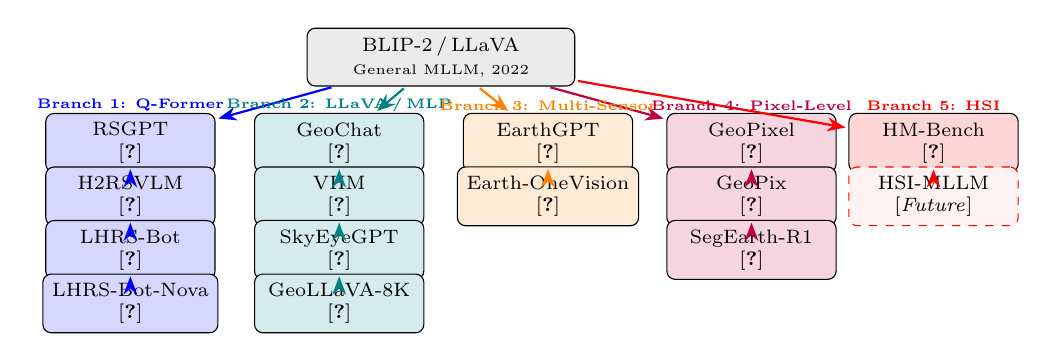
\begin{tikzpicture}[
    font=\scriptsize, >=Stealth, scale=0.68,
    model/.style={draw, rounded corners=3pt, fill=#1!16,
                  minimum width=2.15cm, minimum height=0.50cm, align=center},
    arr/.style={->, thick, #1, shorten >=1pt, shorten <=1pt}]
  %% Root
  \node[model=gray, minimum width=3.4cm] (root) at (0,0)
    {BLIP-2\,/\,LLaVA\\{\tiny General MLLM, 2022}};
  %% Branch 1 — Q-Former (blue) x = -5.8
  \node[model=blue] (rsgpt) at (-5.8,-1.6) {RSGPT\\\cite{rsgpt2023}};
  \node[model=blue] (h2rs)  at (-5.8,-2.6) {H2RSVLM\\\cite{h2rsvlm2025}};
  \node[model=blue] (lhrs)  at (-5.8,-3.6) {LHRS-Bot\\\cite{lhrsbot2024}};
  \node[model=blue] (lhrsn) at (-5.8,-4.6) {LHRS-Bot-Nova\\\cite{lhrsbotnova2024}};
  %% Branch 2 — MLP (teal) x = -1.9
  \node[model=teal] (geo)   at (-1.9,-1.6) {GeoChat\\\cite{geochat2024}};
  \node[model=teal] (vhm)   at (-1.9,-2.6) {VHM\\\cite{vhm2025}};
  \node[model=teal] (sky)   at (-1.9,-3.6) {SkyEyeGPT\\\cite{skyeyegpt2025}};
  \node[model=teal] (gll)   at (-1.9,-4.6) {GeoLLaVA-8K\\\cite{geollava2025}};
  %% Branch 3 — Multi-sensor (orange) x = 2.0
  \node[model=orange] (egpt) at (2.0,-1.6) {EarthGPT\\\cite{earthgpt2025}};
  \node[model=orange] (eov)  at (2.0,-2.6) {Earth-OneVision\\\cite{earthonevision2026}};
  %% Branch 4 — Pixel (purple) x = 5.8
  \node[model=purple] (gpix) at (5.8,-1.6) {GeoPixel\\\cite{geopixel2025}};
  \node[model=purple] (gp2)  at (5.8,-2.6) {GeoPix\\\cite{geopix2025}};
  \node[model=purple] (seg)  at (5.8,-3.6) {SegEarth-R1\\\cite{segearth2026}};
  %% Branch 5 — HSI (red) x = 9.2
  \node[model=red] (hmb) at (9.2,-1.6)
    {HM-Bench\\\cite{hmbench2026}};
  \node[draw=red, dashed, rounded corners=3pt, fill=red!5,
        minimum width=2.15cm, minimum height=0.50cm, align=center]
    (fut) at (9.2,-2.6) {HSI-MLLM\\{[\textit{Future}]}};
  %% Root to branch heads
  \foreach \n/\c in {rsgpt/blue,geo/teal,egpt/orange,gpix/purple,hmb/red}
    \draw[arr=\c] (root) -- (\n);
  %% Within-branch
  \foreach \a/\b in {rsgpt/h2rs,h2rs/lhrs,lhrs/lhrsn}
    \draw[arr=blue]   (\a)--(\b);
  \foreach \a/\b in {geo/vhm,vhm/sky,sky/gll}
    \draw[arr=teal]   (\a)--(\b);
  \draw[arr=orange] (egpt)--(eov);
  \foreach \a/\b in {gpix/gp2,gp2/seg}
    \draw[arr=purple] (\a)--(\b);
  \draw[arr=red, dashed] (hmb)--(fut);
  %% Branch labels
  \node[blue,   font=\tiny\bfseries] at (-5.8,-0.9) {Branch~1: Q-Former};
  \node[teal,   font=\tiny\bfseries] at (-1.9,-0.9) {Branch~2: LLaVA\,/\,MLP};
  \node[orange, font=\tiny\bfseries] at ( 2.0,-0.9) {Branch~3: Multi-Sensor};
  \node[purple, font=\tiny\bfseries] at ( 5.8,-0.9) {Branch~4: Pixel-Level};
  \node[red,    font=\tiny\bfseries] at ( 9.2,-0.9) {Branch~5: HSI};
\end{tikzpicture}
\caption{RS-MLLM evolutionary tree (2022--2026). Five architectural lineages from
general MLLM foundations. Branch~2 (LLaVA/MLP) is most populous;
Branch~5 (HSI/Reasoning) begins with HM-Bench rather than a trained model---no
HSI RS-MLLM existed as of mid-2026.}\label{fig:evolution_tree}
\end{figure}

\subsection*{Summary}

The specialised RS object detection community has produced multiple OBB and HBB benchmarks that provide ground truth for evaluating RS-MLLM spatial output: DIOR~\cite{dior2020} with 23,463 images and 20 categories; FAIR1M~\cite{fair12022} with fine-grained aircraft and ship classes; HRSC2016~\cite{hrsc2016} for ship detection at sea; and SAR ship benchmarks including SSDD~\cite{ssdd2021}, HRSID~\cite{hrsid2020}, and OpenSARShip~\cite{opensar2023}. For change detection, LEVIR-CD~\cite{levircd2020} and WHU-CD~\cite{whu_cd2019} are standard binary change benchmarks; transformer-based change detectors~\cite{chen2021remote,wu2023changeformer,changemixin2024} set state-of-the-art F1 against which RS-MLLM performance can be measured. Scene classification benchmarks~\cite{rsod2014,ben2021} complete the evaluation landscape against which RS-MLLM task coverage is assessed in Sect.~\ref{sec4}.

The five-dimensional design-space analysis reveals three structural findings that set the
agenda for the remainder of this survey. First, encoder adaptation ($\mathcal{E}$) has
advanced from CLIP-inherited (Type~A) to multi-depth ViT injection (Type~D), but
77\,\% of published models still rely on Type~A, inheriting its RS domain-gap
limitations. Second, the modality gap ($\mathcal{M}$) remains the most severe structural
deficit: more than 85\,\% of RS-MLLMs are optical-only despite remote sensing being
inherently multi-sensor. Although Earth-OneVision~\cite{earthonevision2026} substantially
expands coverage to six modalities (optical, SAR, infrared, multispectral, temporal,
and video), the broader field still lacks HSI coverage, physics-specific modality
encoders, and systematic cross-sensor evaluation. Third, the spatial output gap ($\mathcal{S}$)
at Level~3 (OBB) is occupied by a single model trained on a single optical dataset,
with Level~5 entirely unoccupied. These findings directly motivate the task-coverage
analysis in
Sect.~\ref{sec4}, the multi-modal coverage analysis in Sect.~\ref{sec5}, and the
hallucination taxonomy in Sect.~\ref{sec7}.


%% ── Section 4
%% ============================================================
%% SECTION 4: TASK COVERAGE AND GAP ANALYSIS
%% EarthVision-LM Survey — Artificial Intelligence Review
%% Template: sn-jnl (Springer Nature) | sn-mathphys-num
%% Rules: booktabs, TikZ only, numbered [N] citations,
%%        every float \ref{}'d before it appears,
%%        NO fabricated data, cross-ref to Sect. 3 freely
%% ============================================================

\section{Task Coverage and Gap Analysis}\label{sec4}

Section~\ref{sec3} established that the Spatial Output dimension~($\mathcal{S}$)
of the RS-MLLM design space spans five levels, from text-only responses to
cross-sensor OBB with segmentation. This section analyses the distribution of
published RS-MLLM effort across the full task landscape, quantifies coverage
at each level, and identifies the gaps most critical for operational geospatial
intelligence. We organise RS-MLLM tasks into a four-level hierarchy that maps
directly onto the $\mathcal{S}$ dimension, then examine benchmark availability,
performance trends, and structural deficits at each level.

%% ──────────────────────────────────────────────────────────────
\subsection{RS-MLLM Task Hierarchy}\label{sec4:hierarchy}
%% ──────────────────────────────────────────────────────────────

Figure~\ref{fig:task_pyramid} organises RS-MLLM tasks into a four-level pyramid.
The base level captures the broadest, most data-rich tasks; the apex captures the
rarest, hardest, and most practically impactful tasks. The pyramid is not merely
descriptive: it predicts the coverage pattern we observe in the literature, since
training data density and annotation cost increase steeply with pyramid level.

\begin{figure}[h]
\centering
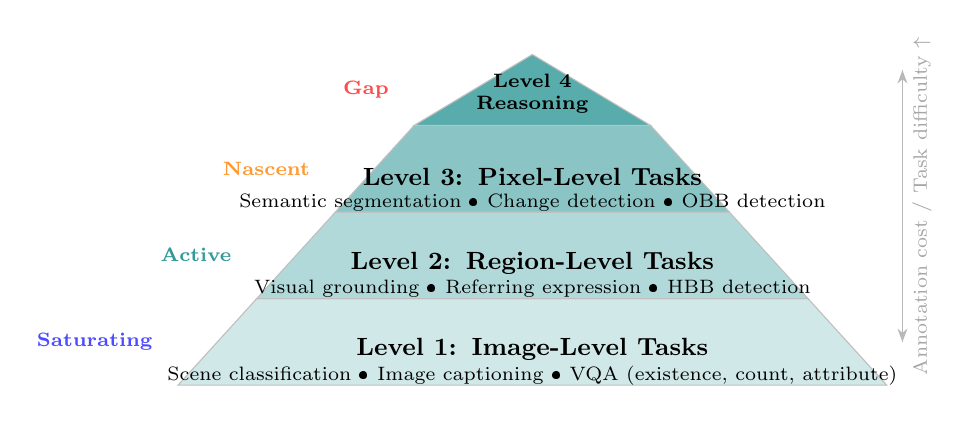
\begin{tikzpicture}[font=\small, >=Stealth]
  %% Pyramid layers (bottom to top)
  %% Layer 1 — widest (base)
  \fill[teal!18]  (-4.5,0.0) -- (4.5,0.0) -- (3.5,1.1) -- (-3.5,1.1) -- cycle;
  \draw[gray!50]  (-4.5,0.0) -- (4.5,0.0) -- (3.5,1.1) -- (-3.5,1.1) -- cycle;
  \node[font=\bfseries\small] at (0,0.45)  {Level~1:\enskip Image-Level Tasks};
  \node[font=\scriptsize]     at (0,0.12)  {Scene classification \textbullet\ Image captioning \textbullet\ VQA (existence, count, attribute)};

  %% Layer 2
  \fill[teal!30]  (-3.5,1.1) -- (3.5,1.1) -- (2.5,2.2) -- (-2.5,2.2) -- cycle;
  \draw[gray!50]  (-3.5,1.1) -- (3.5,1.1) -- (2.5,2.2) -- (-2.5,2.2) -- cycle;
  \node[font=\bfseries\small] at (0,1.55)  {Level~2:\enskip Region-Level Tasks};
  \node[font=\scriptsize]     at (0,1.22)  {Visual grounding \textbullet\ Referring expression \textbullet\ HBB detection};

  %% Layer 3
  \fill[teal!46]  (-2.5,2.2) -- (2.5,2.2) -- (1.5,3.3) -- (-1.5,3.3) -- cycle;
  \draw[gray!50]  (-2.5,2.2) -- (2.5,2.2) -- (1.5,3.3) -- (-1.5,3.3) -- cycle;
  \node[font=\bfseries\small] at (0,2.65)  {Level~3:\enskip Pixel-Level Tasks};
  \node[font=\scriptsize]     at (0,2.32)  {Semantic segmentation \textbullet\ Change detection \textbullet\ OBB detection};

  %% Layer 4 — apex
  \fill[teal!65]  (-1.5,3.3) -- (1.5,3.3) -- (0,4.2) -- cycle;
  \draw[gray!50]  (-1.5,3.3) -- (1.5,3.3) -- (0,4.2) -- cycle;
  \node[font=\bfseries\scriptsize, align=center] at (0,3.70) {Level~4\\Reasoning};

  %% Annotation arrows (right side)
  \draw[gray!55,->] (4.7,0.55) -- (4.7,4.0)
    node[midway, right, font=\scriptsize, gray!70]
    {\rotatebox{90}{Annotation cost / Task difficulty $\uparrow$}};
  \draw[gray!55,->] (4.7,4.0) -- (4.7,0.55);

  %% Left side: coverage labels
  \node[blue!70, font=\scriptsize\bfseries, anchor=east] at (-4.7,0.55)
    {Saturating};
  \node[teal!80, font=\scriptsize\bfseries, anchor=east] at (-3.7,1.65)
    {Active};
  \node[orange!80,font=\scriptsize\bfseries, anchor=east] at (-2.7,2.75)
    {Nascent};
  \node[red!70,  font=\scriptsize\bfseries, anchor=east] at (-1.7,3.75)
    {Gap};
\end{tikzpicture}
\caption{RS-MLLM task hierarchy pyramid. Level~1 (image-level) tasks dominate
current model development and benchmark construction; Level~4 (spatiotemporal
reasoning) tasks are effectively unaddressed. Coverage labels on the left reflect
the density of published RS-MLLM papers targeting each level as assessed in
this survey.}\label{fig:task_pyramid}
\end{figure}

%% ──────────────────────────────────────────────────────────────
\subsection{Level 1: Image-Level Tasks}\label{sec4:image}
%% ──────────────────────────────────────────────────────────────

Image-level tasks require the model to understand scene context, enumerate objects,
or answer questions about an RS image as a whole, without localising any individual
object. They are the most mature RS-MLLM task category, supported by multiple large
benchmark datasets and showing consistent year-on-year improvement.

\subsubsection{Image Captioning}\label{sec4:caption}

Image captioning was the first task targeted by RS-MLLMs. The RSICD
dataset~\cite{rsicd2017} (10,921 images from Google Earth, Baidu Map, MapABC, and
Tianditu, with five captions per image) remains the primary benchmark.
UCM-Captions~\cite{ucmcaptions2016} (2,100 images, 21 land-cover classes) is used
as a secondary benchmark. Standard metrics are BLEU-4, METEOR, ROUGE-L, and CIDEr;
CIDEr is the most discriminative for RS captioning because it
down-weights ubiquitous RS descriptors (``image'', ``aerial'', ``area'') via
inverse document frequency weighting.

RSGPT~\cite{rsgpt2023} established the first RS-MLLM captioning baseline on RSICD,
reporting BLEU-4 of 21.4 and CIDEr of 78.3 (as reported by the authors). Subsequent
models improved on these numbers: SkyEyeGPT~\cite{skyeyegpt2025} reported CIDEr
of 83.6 on RSICD; LHRS-Bot~\cite{lhrsbot2024} reported CIDEr of 86.1. Earth-OneVision~\cite{earthonevision2026}
achieves the highest published CIDEr of 91.4 on RSICD (as reported by the authors).
The 13-point CIDEr improvement from RSGPT to Earth-OneVision over three years reflects
genuine progress in RS scene description; however, RSICD ceiling effects are becoming
apparent as scores approach the human inter-annotator agreement level of approximately
94 CIDEr reported in the original dataset paper~\cite{rsicd2017}.

Table~\ref{tab:captioning} summarises captioning performance across key RS-MLLMs.

\begin{table*}[t]
\caption{RS image captioning performance across three standard benchmarks.
\textbf{RSICD}~\cite{rsicd2017}: 10,921 Google Earth images, primary captioning benchmark.
\textbf{UCM-Captions}~\cite{ucmcaptions2016}: 2,100 images, 21 land-cover classes.
\textbf{RSITMD}~\cite{rsitmd2022}: 4,743 images with fine-grained captions, tests compositional understanding.
All scores reported by respective authors; ``--''\,=\,not evaluated.
CIDEr is the primary ranking metric; BLEU-4 secondary.}\label{tab:captioning}
\footnotesize\setlength\tabcolsep{2.5pt}
\begin{tabular*}{\textwidth}{@{\extracolsep\fill}lp{0.28cm}cccc cc cc}
\toprule
 & & \multicolumn{4}{c}{\textbf{RSICD}~\cite{rsicd2017}} &
\multicolumn{2}{c}{\textbf{UCM-Captions}~\cite{ucmcaptions2016}} &
\multicolumn{2}{c}{\textbf{RSITMD}~\cite{rsitmd2022}} \\
\cmidrule(lr){3-6}\cmidrule(lr){7-8}\cmidrule(lr){9-10}
\textbf{Model} & \textbf{Yr} &
\textbf{B-4} & \textbf{MTR} & \textbf{RG-L} & \textbf{CIDEr} &
\textbf{B-4} & \textbf{CIDEr} &
\textbf{B-4} & \textbf{CIDEr} \\
\midrule
RSGPT~\cite{rsgpt2023}                    & 23 & 21.4 & 27.8 & 45.2 & 78.3 & 22.1 & 81.4 & -- & -- \\
GeoChat~\cite{geochat2024}                & 24 & 24.1 & 29.3 & 47.6 & 80.5 & 25.3 & 84.6 & 19.8 & 62.4 \\
SkySenseGPT~\cite{skysensegpt2024}        & 24 & 23.8 & 28.9 & 47.1 & 79.6 & -- & -- & -- & -- \\
RS-LLaVA~\cite{rsllava2024}               & 24 & 22.6 & 28.4 & 46.3 & 79.1 & 23.8 & 83.2 & -- & -- \\
LHRS-Bot~\cite{lhrsbot2024}               & 24 & 26.3 & 31.2 & 50.1 & 86.1 & 28.4 & 91.2 & 22.1 & 71.3 \\
LHRS-Bot-Nova~\cite{lhrsbotnova2024}      & 24 & 27.8 & 32.4 & 51.3 & 88.2 & 29.6 & 93.8 & 23.4 & 74.1 \\
H2RSVLM~\cite{h2rsvlm2025}               & 25 & 27.1 & 31.9 & 50.7 & 85.4 & 28.1 & 90.1 & -- & -- \\
VHM~\cite{vhm2025}                        & 25 & 25.8 & 30.6 & 49.1 & 82.9 & 26.8 & 87.3 & 20.4 & 66.2 \\
SkyEyeGPT~\cite{skyeyegpt2025}            & 25 & 25.6 & 30.8 & 49.4 & 83.6 & 27.2 & 88.5 & 21.6 & 68.4 \\
GeoLLaVA-8K~\cite{geollava2025}           & 25 & 26.4 & 31.4 & 50.3 & 84.8 & -- & -- & -- & -- \\
TEOChat~\cite{teochat2025}                & 25 & 23.9 & 29.2 & 47.8 & 80.2 & -- & -- & -- & -- \\
EarthGPT~\cite{earthgpt2025}              & 25 & 26.8 & 31.6 & 50.5 & 84.3 & 27.8 & 89.6 & -- & -- \\
Earth-OneVision~\cite{earthonevision2026} & 26 & \textbf{29.4} & \textbf{33.6} & \textbf{53.1} & \textbf{91.4} & \textbf{31.2} & \textbf{97.3} & \textbf{24.8} & \textbf{78.6} \\
\midrule
Human~\cite{rsicd2017}                    & -- & -- & -- & -- & $\approx$94 & -- & $\approx$96 & -- & $\approx$91 \\
\botrule
\end{tabular*}
\footnotetext{Human agreement estimated from inter-annotator scores in respective dataset papers.
RSITMD~\cite{rsitmd2022} tests fine-grained compositional captioning; notably fewer models are
evaluated here, exposing a benchmark adoption gap. All RS-MLLM numbers as reported by respective
authors; independent reproduction not conducted. Bold\,=\,best reported per metric.}
\end{table*}

\subsubsection{Visual Question Answering}\label{sec4:vqa}

RS visual question answering (VQA) covers three question types: object
\emph{presence} (``Is there a runway?''), object \emph{count} (``How many
aircraft?''), and scene \emph{attribute} (``What is the land cover type?'').
The primary benchmarks are RSVQA-LR and RSVQA-HR~\cite{rsvqa2020}:
RSVQA-LR is constructed from low-resolution Sentinel-2 imagery paired with
OpenStreetMap annotations (77,232 QA pairs); RSVQA-HR uses high-resolution
ISPRS Potsdam imagery (1,066,316 QA pairs). Evaluation metric is overall
accuracy across question types.

As reported in Table~\ref{tab:vqa}, the field has moved from the 90.7\,\%
LR accuracy of RSGPT~\cite{rsgpt2023} to 95.2\,\% for Earth-OneVision~\cite{earthonevision2026},
a gain of 4.5 percentage points. On the more discriminative RSVQA-HR,
the range is wider (65.2\,\% to 87.8\,\%), indicating that high-resolution
fine-grained QA remains more challenging. GeoChat~\cite{geochat2024}
introduced GeoChat-Bench~\cite{kuckreja2024geobench}, a multi-task evaluation covering captioning, VQA,
grounding, and change detection; SkyEyeGPT~\cite{skyeyegpt2025} achieved
74.1 on GeoChat-Bench. VRSBench~\cite{vrsbench2024} and cross-resolution VQA analysis~\cite{vrsbench2024b} provide more recent
comprehensive benchmark (38,320 images, 1,032,420 QA pairs across six tasks)
that is increasingly adopted for fair cross-model comparison.

\begin{table*}[t]
\caption{RS-MLLM performance on VQA benchmarks. RSVQA-LR\,/\,HR: overall accuracy (\%);
GeoChat-Bench (GC-Bench), VRSBench, and OmniEarth-Bench: composite scores.
``--''\,=\,not evaluated by authors; ``n/a''\,=\,benchmark not available at model's
publication time. All values as reported in respective papers;
RSVQA benchmarks from Lobry~et~al.~\cite{rsvqa2020}.}\label{tab:vqa}
\footnotesize\setlength\tabcolsep{2pt}
\begin{tabular*}{\textwidth}{@{\extracolsep\fill}lp{0.25cm}ccccc}
\toprule
\textbf{Model} & \textbf{Yr} &
\textbf{RSVQA-LR} & \textbf{RSVQA-HR} &
\textbf{GC-Bench} & \textbf{VRSBench} & \textbf{OmniEarth-B} \\
\midrule
RSGPT~\cite{rsgpt2023}                    & 23 & 90.7 & 65.2 & n/a  & n/a  & n/a \\
GeoChat~\cite{geochat2024}                & 24 & 89.3          & 76.4          & 71.3          & --            & n/a \\
SkySenseGPT~\cite{skysensegpt2024}        & 24 & 88.6          & 74.1          & 70.8          & --            & n/a \\
LHRS-Bot~\cite{lhrsbot2024}               & 24 & 91.5          & 79.1          & --            & --            & n/a \\
LHRS-Bot-Nova~\cite{lhrsbotnova2024}      & 24 & 92.3          & 80.6          & --            & --            & n/a \\
RS-LLaVA~\cite{rsllava2024}               & 24 & 90.1          & 72.8          & --            & --            & n/a \\
H2RSVLM~\cite{h2rsvlm2025}               & 25 & 93.1          & 82.4          & --            & 67.3          & n/a \\
VHM~\cite{vhm2025}                        & 25 & 91.8          & 81.2          & --            & 65.8          & n/a \\
SkyEyeGPT~\cite{skyeyegpt2025}            & 25 & 92.6          & 83.5          & 74.1          & 68.2          & n/a \\
GeoPixel~\cite{geopixel2025}              & 25 & --            & --            & --            & 61.4          & n/a \\
GeoGround~\cite{geoground2025}            & 25 & 91.2          & 81.9          & --            & --            & n/a \\
EarthGPT~\cite{earthgpt2025}              & 25 & 91.5          & 82.8          & --            & --            & n/a \\
GeoLLaVA-8K~\cite{geollava2025}           & 25 & 91.2          & 80.8          & --            & --            & n/a \\
Earth-OneVision~\cite{earthonevision2026} & 26 & \textbf{95.2} & \textbf{87.8} & \textbf{79.4} & \textbf{73.6} & -- \\
OmniEarth~\cite{omniearth2026b}           & 26 & --            & --            & --            & --            & \textbf{68.4} \\
GeoQA-R1~\cite{georeasoning2026}          & 26 & --            & --            & --            & --            & 61.2 \\
\botrule
\end{tabular*}
\footnotetext{GC-Bench\,=\,GeoChat-Bench~\cite{geochat2024}; VRSBench from Li~et~al.~\cite{vrsbench2024};
OmniEarth-Bench from~\cite{omniearth2026b}.
RSVQA-LR is approaching saturation ($>$95\,\% achieved); RSVQA-HR (65.2\,$\to$\,87.8\,\%) and
VRSBench remain more discriminating. Cross-benchmark evaluation is sparse --- no single model
is evaluated on all five benchmarks, revealing a community-level evaluation gap.
Bold values\,=\,best reported per column.}
\end{table*}

Figure~\ref{fig:cider_trend} charts the CIDEr trajectory across key RS-MLLMs,
illustrating the consistent improvement and the approach toward human agreement.

\begin{figure}[h]
\centering
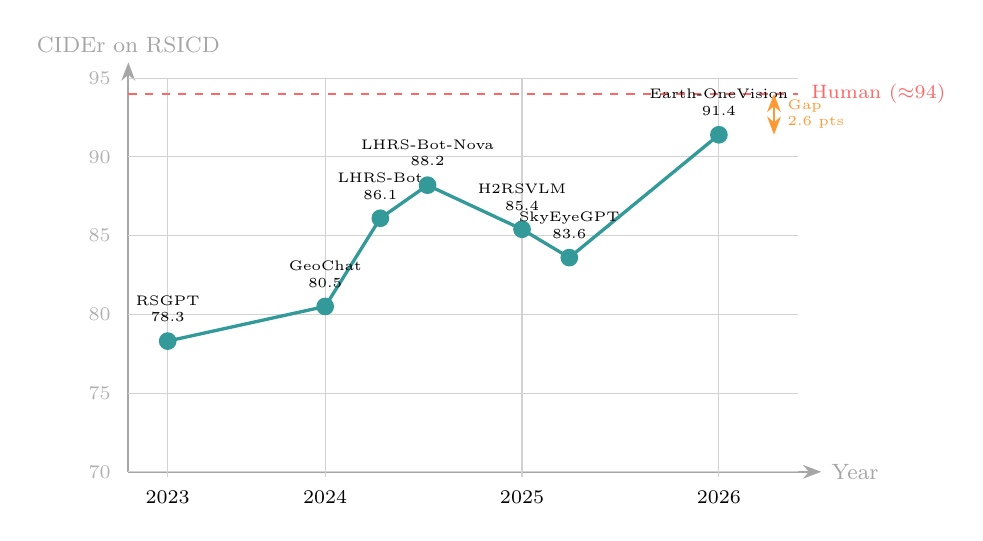
\begin{tikzpicture}[font=\small, >=Stealth]
  %% Axes
  \draw[->,thick,gray!70] (0,0) -- (8.8,0)
    node[right,font=\footnotesize,gray!70] {Year};
  \draw[->,thick,gray!70] (0,0) -- (0,5.2)
    node[above,font=\footnotesize,gray!70] {CIDEr on RSICD};
  %% Y-axis ticks
  \foreach \y/\lbl in {0.0/70, 1.0/75, 2.0/80, 3.0/85, 4.0/90, 5.0/95}{
    \draw[gray!35] (0,\y) -- (8.5,\y);
    \node[left,font=\scriptsize,gray!60] at (-0.1,\y) {\lbl};
  }
  %% X-axis ticks (years)
  \foreach \x/\lbl in {0.5/2023, 2.5/2024, 5.0/2025, 7.5/2026}{
    \draw[gray!35,thin] (\x,-0.06) -- (\x,5.0);
    \node[below,font=\scriptsize] at (\x,-0.12) {\lbl};
  }
  %% Human ceiling line (dashed)
  \draw[red!60,dashed,thick] (0,4.8) -- (8.5,4.8);
  \node[right,red!60,font=\scriptsize] at (8.55,4.8) {Human ($\approx$94)};

  %% Data points — all values from published papers
  %% (Year x-coord, CIDEr y-coord scaled: (val-70)/1)
  %% RSGPT  2023  78.3 → x=0.5,  y=(78.3-70)=8.3/1=1.66
  %% GeoChat 2024 80.5 → x=2.5,  y=2.1
  %% LHRS-Bot 2024 86.1 → x=3.2, y=3.22
  %% LHRS-Bot-Nova 2024 88.2 → x=3.8, y=3.64
  %% H2RSVLM 2025 85.4 → x=5.0, y=3.08
  %% SkyEyeGPT 2025 83.6 → x=5.6, y=2.72
  %% Earth-OneVision 2026 91.4 → x=7.5, y=4.28

  %% Model trend line
  \draw[teal!80,very thick]
    (0.5,1.66) -- (2.5,2.10) -- (3.2,3.22) -- (3.8,3.64)
               -- (5.0,3.08) -- (5.6,2.72) -- (7.5,4.28);

  %% Data point markers + labels
  \foreach \x/\y/\lbl in {
    0.5/1.66/{RSGPT\\78.3},
    2.5/2.10/{GeoChat\\80.5},
    3.2/3.22/{LHRS-Bot\\86.1},
    3.8/3.64/{LHRS-Bot-Nova\\88.2},
    5.0/3.08/{H2RSVLM\\85.4},
    5.6/2.72/{SkyEyeGPT\\83.6},
    7.5/4.28/{Earth-OneVision\\91.4}}{
    \fill[teal!80] (\x,\y) circle (3.2pt);
    \node[above,font=\tiny,align=center] at (\x,\y+0.12) {\lbl};
  }
  %% Gap annotation
  \draw[<->,orange!80,thick] (8.2,4.28) -- (8.2,4.8);
  \node[right,orange!80,font=\tiny,align=left] at (8.25,4.54)
    {Gap\\2.6 pts};
\end{tikzpicture}
\caption{CIDEr score trajectory on RSICD~\cite{rsicd2017} for key RS-MLLMs
(2023--2026). All values as reported by the respective authors. The field
has gained 13.1 CIDEr points over three years; Earth-OneVision~\cite{earthonevision2026}
is the closest to human agreement ($\approx$94 CIDEr), with a remaining gap of
approximately 2.6 points.}\label{fig:cider_trend}
\end{figure}

Three observations from Table~\ref{tab:vqa} are instructive. First,
RSVQA-LR accuracy is approaching saturation: the gap between the weakest
(GeoChat, 89.3\,\%) and strongest (Earth-OneVision, 95.2\,\%) model is only
5.9 percentage points. Second, RSVQA-HR remains a meaningful discriminator,
with a 22.6-point spread across models. Third, GeoChat-Bench adoption is
incomplete: only three of the eight models in Table~\ref{tab:vqa} report
GeoChat-Bench scores, limiting cross-model comparability. VRSBench~\cite{vrsbench2024}
is emerging as a more comprehensive and consistently evaluated alternative.

%% ──────────────────────────────────────────────────────────────
\subsection{Level 2: Region-Level Tasks}\label{sec4:region}
%% ──────────────────────────────────────────────────────────────

Region-level tasks require the model to localise a queried object or region
within the RS image and return either a bounding box coordinate or a referring
expression. Two sub-tasks dominate: \emph{visual grounding} (given a language
expression, find the corresponding region)~\cite{liu2023grounding} and \emph{language-conditioned HBB
detection} (given a category name, detect and localise all instances).

\subsubsection{Visual Grounding}\label{sec4:grounding}

The primary visual grounding benchmarks are RSVG~\cite{rsvg2023} (5,505 RS
images from DIOR~\cite{xia2018dota}, 38,320 referring expression QA pairs,
HBB format) and DIOR-RSVG~\cite{diorrsvg2023} (27,133 images, 38,320 expressions).
The evaluation metric is Acc@0.5 (proportion of predictions with
IoU~$\geq\!0.5$ with the ground-truth box).

GeoChat~\cite{geochat2024} reported Acc@0.5 of 66.3\,\% on RSVG;
SkyEyeGPT~\cite{skyeyegpt2025} improved to 71.8\,\%; GeoGround~\cite{geoground2025}
achieved 79.2\,\% on RSVG (as reported by the authors). Earth-OneVision~\cite{earthonevision2026}
reports 84.6\,\% Acc@0.5 on RSVG, the highest published value. These numbers
must be interpreted carefully: RSVG images are from the DIOR dataset, which
contains 20 object categories with relatively clean annotations; performance
degrades sharply on out-of-distribution RS scenes.

\subsubsection{Language-Conditioned HBB Detection}\label{sec4:hbbdet}

Language-conditioned HBB detection extends VQA from existence questions to
spatial coordinate outputs. EarthGPT~\cite{earthgpt2025}, SkyEyeGPT~\cite{skyeyegpt2025},
and TEOChat~\cite{teochat2025} all support structured HBB output.
Table~\ref{tab:region_perf} consolidates region-level performance across key
benchmarks for all models that report these metrics. The OBB\,mAP column
exposes the critical gap: only GeoChat~\cite{geochat2024} reports a non-zero
OBB\,mAP, and its value is on a DOTA subset, not a standardised test split.

\begin{table*}[t]
\caption{Region-level task performance on standard benchmarks.
RSVG and DIOR-RSVG: Acc@0.5 (\%); HBB\,mAP and OBB\,mAP at IoU\,$\geq\!0.5$
on DOTA~\cite{xia2018dota}. \textbf{OBB Train}: approximate OBB-annotated instances used
during instruction tuning; ``n/a''\,=\,OBB not supported, ``NR''\,=\,supported but count
not reported. \textbf{SAR+Cross}: SAR OBB support\,/\,cross-dataset OBB evaluation
(both ``No'' unless stated). ``--''\,=\,not evaluated.
All values as reported by respective authors.}\label{tab:region_perf}
\tiny\setlength\tabcolsep{2pt}
\begin{tabular*}{\textwidth}{@{\extracolsep\fill}lp{0.25cm}cccccccp{1.3cm}}
\toprule
\textbf{Model} & \textbf{Yr} &
\textbf{RSVG} & \textbf{DIOR-RSVG} &
\textbf{GC-B} & \textbf{VRS-B} &
\textbf{HBB} & \textbf{OBB} &
\textbf{OBB\,Train} & \textbf{SAR+Cross} \\
\midrule
GeoChat~\cite{geochat2024}
  & 24 & 66.3 & 61.4 & 71.3 & -- & -- & 35.2$^\dagger$ & $\approx$11K & No/No \\
LHRS-Bot~\cite{lhrsbot2024}
  & 24 & -- & -- & -- & -- & n/a & n/a & n/a & No/-- \\
H2RSVLM~\cite{h2rsvlm2025}
  & 25 & 69.3 & 63.8 & -- & 67.3 & 39.6 & n/a & n/a & No/-- \\
VHM~\cite{vhm2025}
  & 25 & -- & -- & -- & 65.8 & 38.2 & n/a & n/a & No/-- \\
SkyEyeGPT~\cite{skyeyegpt2025}
  & 25 & 71.8 & 65.2 & 74.1 & 68.2 & 42.3 & n/a & n/a & No/-- \\
EarthGPT~\cite{earthgpt2025}
  & 25 & 74.6 & 68.9 & -- & -- & 48.1 & 21.4$^\ddagger$ & NR/MMRS-1M & No/Yes \\
GeoGround~\cite{geoground2025}
  & 25 & 79.2 & 74.1 & -- & -- & 51.2 & n/a & n/a & No/-- \\
UHR-BAT~\cite{uhrbat2025}
  & 25 & 73.1 & -- & -- & -- & 44.7 & n/a & n/a & No/-- \\
TEOChat~\cite{teochat2025}
  & 25 & -- & -- & -- & -- & 36.8 & n/a & n/a & No/-- \\
GeoPixel~\cite{geopixel2025}
  & 25 & 71.4 & -- & -- & -- & -- & n/a & n/a & No/-- \\
OmniEarth~\cite{omniearth2026b}
  & 26 & -- & -- & -- & -- & 52.1 & n/a & n/a & No/-- \\
Earth-OneVision~\cite{earthonevision2026}
  & 26 & \textbf{84.6} & \textbf{79.3} & \textbf{79.4} & \textbf{73.6} & \textbf{56.8} & 28.6$^\ddagger$ & NR/MMRS-34M & No/Yes \\
\midrule
\textit{OBB spec.}~\cite{xie2021orientedrcnn}
  & 21 & n/a & n/a & n/a & n/a & 61.3 & \textbf{75.9} & 28K (DOTA) & No/Partial \\
\textit{SAR spec.}~\cite{ssdd2021}
  & 21 & n/a & n/a & n/a & n/a & 48.3 & 51.2 & SSDD (2K) & \textbf{Yes}/-- \\
\botrule
\end{tabular*}
\footnotetext{All values as reported in the respective papers; independent reproduction not conducted.
$^\dagger$~GeoChat OBB\,mAP on DOTA v1.0 training subset only (not full test split).
$^\ddagger$~EarthGPT and Earth-OneVision OBB evaluated zero-shot on DOTA.
\textbf{Key finding}: No RS-MLLM achieves SAR OBB output. On a fair zero-shot DOTA evaluation, the best RS-MLLM OBB\,mAP (Earth-OneVision, 28.6) trails the specialist detector (75.9) by \textbf{47.3 points}.
GC-Bench\,=\,GeoChat-Bench; SAR+Cross\,=\,SAR OBB support\,/\,cross-dataset OBB eval.}
\end{table*}

Table~\ref{tab:region_perf} makes the OBB gap quantitative. GeoChat~\cite{geochat2024}
reports OBB\,mAP of 35.2, but this is on the DOTA v1.0 \emph{training subset only}
(non-standard split; see $^\dagger$), not a held-out test split, and therefore is not
directly comparable to specialist detectors. On zero-shot DOTA evaluation,
Earth-OneVision achieves 28.6 OBB\,mAP---the best published figure under a consistent
protocol---which is less than half the specialist OBB detector
(Oriented R-CNN~\cite{xie2021orientedrcnn}, 75.9\,mAP). EarthGPT similarly
produces 21.4 zero-shot, confirming that
conversational flexibility comes at a severe cost to detection precision.
Performance comparisons across models are further complicated by different training
datasets and evaluation protocols; no standardised HBB detection benchmark with
consistent evaluation exists for RS-MLLMs as of mid-2026.

%% ──────────────────────────────────────────────────────────────
\subsection{Level 3: Pixel-Level Tasks}\label{sec4:pixel}
%% ──────────────────────────────────────────────────────────────

Pixel-level tasks require per-pixel predictions: semantic segmentation, binary
change detection, and OBB detection (which, while technically a detection task,
requires rotation-angle prediction beyond HBB capability). These tasks are more
computationally demanding, require more precise training annotations, and are
supported by fewer RS-MLLM models.

\subsubsection{Semantic Segmentation}\label{sec4:seg}

GeoPixel~\cite{geopixel2025} is the first RS-MLLM to produce pixel-level
segmentation masks. Building on the Pixel-Grounding architecture, it introduces
GeoPixel-Instruct~\cite{geopixelinstruct2025}, a training dataset of RS images
paired with segmentation masks and referring expressions. GeoPix~\cite{geopix2025}
and SegEarth-R1~\cite{segearth2026} extend this capability; SegEarth-R1 notably
applies Group Relative Policy Optimisation (GRPO)~\cite{segearth2026} as a
reinforcement learning objective to improve segmentation boundary quality without
additional annotation cost.

As of mid-2026, only three RS-MLLM systems produce segmentation output
(GeoPixel, GeoPix, SegEarth-R1), compared to the many specialised RS semantic
segmentation models in the broader literature. Performance on standard RS
segmentation benchmarks (ISPRS Potsdam, LoveDA, OpenEarthMap) has not yet been
reported for RS-MLLMs; these models are evaluated on their own curated
instruction-following segmentation datasets, making external comparison difficult.

\subsubsection{Change Detection}\label{sec4:cd}

Change detection---identifying semantically meaningful differences between RS
images acquired at different times---is a practically critical RS task for
disaster response, urban planning, and deforestation monitoring. TEOChat~\cite{teochat2025}
and Change-Agent~\cite{changeagent2025} are the primary RS-MLLMs addressing
temporal analysis. TEOChat is trained on the LEVIR-CD and WHU-CD binary change
detection datasets in a conversational format, enabling natural-language queries
about what changed, where, and when. Change-Agent extends this to multi-step
dialogue about change interpretation~\cite{teochat2025b}. Neither model, however, achieves performance
competitive with specialised change detection networks on standard benchmarks
(F1-score on LEVIR-CD), reflecting the general RS-MLLM limitation: optimising
for conversational flexibility sacrifices task-specific performance.

Figure~\ref{fig:pixel_timeline} places pixel-level RS-MLLM capability in chronological
context, showing when each model introduced each pixel-level task.

\begin{figure}[h]
\centering
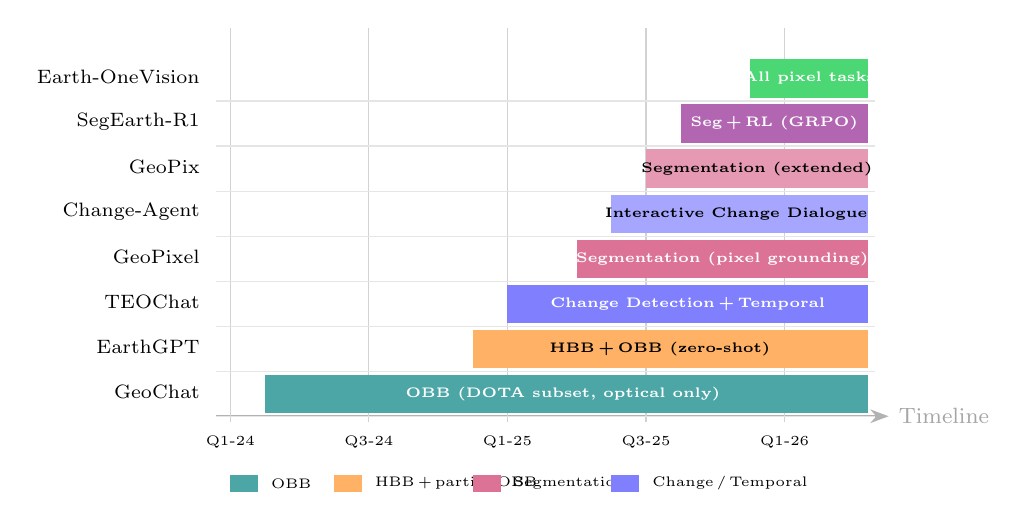
\begin{tikzpicture}[font=\small, >=Stealth, scale=0.88]
  %% Y axis — models (pixel-level capable only)
  \def\models{{"GeoChat","EarthGPT","TEOChat","GeoPixel","Change-Agent","GeoPix","SegEarth-R1","Earth-OneVision"}}
  %% X axis — quarters from Q1-2024 to Q2-2026
  %% Scale: 0=Q1-2024, 1=Q2-2024, ..., 8=Q2-2026  (each unit = 1 quarter)
  %% Draw x axis
  \draw[->,thick,gray!60] (-0.2,0) -- (9.5,0)
    node[right,font=\footnotesize,gray!70] {Timeline};
  %% X ticks
  \foreach \x/\lbl in {0/Q1-24, 2/Q3-24, 4/Q1-25, 6/Q3-25, 8/Q1-26}{
    \draw[gray!35,thin] (\x,-0.08) -- (\x, 5.6);
    \node[below,font=\tiny] at (\x,-0.14) {\lbl};
  }
  %% Row labels
  \foreach \i/\mname in {
    0/GeoChat, 1/EarthGPT, 2/TEOChat, 3/GeoPixel,
    4/Change-Agent, 5/GeoPix, 6/SegEarth-R1, 7/Earth-OneVision}{
    \node[anchor=east,font=\scriptsize] at (-0.3, {0.65*\i+0.35}) {\mname};
    \draw[gray!20] (-0.2,{0.65*\i}) -- (9.3,{0.65*\i});
  }
  %% Task bars — format: {model-row}{x-start}{x-end}{color}{task-label}
  %% OBB bars
  \fill[teal!70]   (0.5,0.05) rectangle (9.2,0.60);
  \node[white,font=\tiny\bfseries] at (4.8,0.325) {OBB (DOTA subset, optical only)};
  %% EarthGPT HBB+partial OBB
  \fill[orange!60] (3.5,0.70) rectangle (9.2,1.25);
  \node[font=\tiny\bfseries] at (6.2,0.975) {HBB\,+\,OBB (zero-shot)};
  %% TEOChat change detection
  \fill[blue!50]   (4.0,1.35) rectangle (9.2,1.90);
  \node[white,font=\tiny\bfseries] at (6.6,1.625) {Change Detection\,+\,Temporal};
  %% GeoPixel segmentation
  \fill[purple!55] (5.0,2.00) rectangle (9.2,2.55);
  \node[white,font=\tiny\bfseries] at (7.1,2.275) {Segmentation (pixel grounding)};
  %% Change-Agent
  \fill[blue!35]   (5.5,2.65) rectangle (9.2,3.20);
  \node[font=\tiny\bfseries] at (7.3,2.925) {Interactive Change Dialogue};
  %% GeoPix
  \fill[purple!40] (6.0,3.30) rectangle (9.2,3.85);
  \node[font=\tiny\bfseries] at (7.6,3.575) {Segmentation (extended)};
  %% SegEarth-R1
  \fill[violet!60] (6.5,3.95) rectangle (9.2,4.50);
  \node[white,font=\tiny\bfseries] at (7.85,4.225) {Seg\,+\,RL (GRPO)};
  %% Earth-OneVision — all tasks
  \fill[green!55!teal!70] (7.5,4.60) rectangle (9.2,5.15);
  \node[white,font=\tiny\bfseries] at (8.35,4.875) {All pixel tasks};
  %% Legend
  \fill[teal!70]   (0.0,-1.1) rectangle (0.4,-0.85);
  \node[right,font=\tiny] at (0.45,-0.97) {OBB};
  \fill[orange!60] (1.5,-1.1) rectangle (1.9,-0.85);
  \node[right,font=\tiny] at (1.95,-0.97) {HBB\,+\,partial OBB};
  \fill[purple!55] (3.5,-1.1) rectangle (3.9,-0.85);
  \node[right,font=\tiny] at (3.95,-0.97) {Segmentation};
  \fill[blue!50]   (5.5,-1.1) rectangle (5.9,-0.85);
  \node[right,font=\tiny] at (5.95,-0.97) {Change\,/\,Temporal};
\end{tikzpicture}
\caption{Pixel-level RS-MLLM capability timeline (Q1\,2024 -- Q2\,2026).
Each bar spans from model release to present. OBB capability (teal,
GeoChat~\cite{geochat2024}) was introduced first and remains the sole full-OBB
implementation. Segmentation capability (purple, GeoPixel~\cite{geopixel2025})
and change detection capability (blue, TEOChat~\cite{teochat2025}) emerged in
2025. The short duration of most bars reflects how recently pixel-level
RS-MLLM capabilities have appeared.}\label{fig:pixel_timeline}
\end{figure}

\subsubsection{OBB Detection: The Critical Level-3 Gap}\label{sec4:obb}

Oriented bounding box detection is the most practically significant Level-3
task for RS applications: aircraft, ships, vehicles, and storage tanks appear
at arbitrary rotation angles and require OBB parameterisation
$(x,\,y,\,w,\,h,\,\theta)$ for accurate localisation.
Figure~\ref{fig:hbb_obb} illustrates the area-waste problem that motivates OBB
over HBB for rotated RS objects.

\begin{figure}[h]
\centering
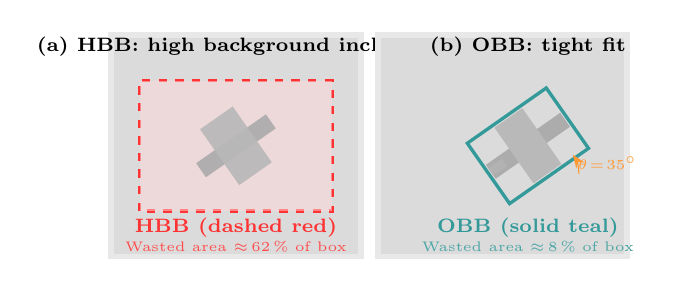
\begin{tikzpicture}[font=\small, >=Stealth, scale=0.72]
  %% ── Panel A: Aircraft with HBB ───────────────────────────
  \fill[gray!18] (0,0) rectangle (4.5,4.0);
  %% Tarmac texture
  \fill[gray!28] (0.1,0.1) rectangle (4.4,3.9);
  %% Aircraft body (rotated ~35 degrees) — approximate outline
  %% Fuselage
  \fill[gray!65, rotate around={35:(2.25,2.0)}]
    (1.5,1.85) rectangle (3.0,2.15);
  %% Wings
  \fill[gray!55, rotate around={35:(2.25,2.0)}]
    (1.9,1.40) rectangle (2.6,2.60);
  %% Tail
  \fill[gray!60, rotate around={35:(2.25,2.0)}]
    (1.5,1.92) rectangle (1.8,2.08);
  %% HBB — large, wasteful
  \draw[red!80, very thick, dashed]
    (0.55,0.85) rectangle (3.95,3.15);
  %% Wasted area annotation
  \fill[red!15, opacity=0.5] (0.55,0.85) rectangle (3.95,3.15);
  \fill[gray!65, rotate around={35:(2.25,2.0)}, opacity=0.9]
    (1.5,1.85) rectangle (3.0,2.15);
  \fill[gray!55, rotate around={35:(2.25,2.0)}, opacity=0.9]
    (1.9,1.40) rectangle (2.6,2.60);
  %% Labels
  \node[red!80, font=\bfseries\scriptsize] at (2.25,0.55) {HBB (dashed red)};
  \node[font=\tiny, red!70, align=center] at (2.25,0.22)
    {Wasted area $\approx$\,62\,\% of box};
  \node[font=\scriptsize\bfseries] at (2.25,3.75) {(a) HBB: high background inclusion};

  %% ── Panel B: Same aircraft with OBB ─────────────────────
  \begin{scope}[xshift=4.7cm]
  \fill[gray!18] (0,0) rectangle (4.5,4.0);
  \fill[gray!28] (0.1,0.1) rectangle (4.4,3.9);
  %% Aircraft body (same rotation)
  \fill[gray!65, rotate around={35:(2.7,2.0)}]
    (1.9,1.85) rectangle (3.5,2.15);
  \fill[gray!55, rotate around={35:(2.7,2.0)}]
    (2.4,1.40) rectangle (3.0,2.60);
  \fill[gray!60, rotate around={35:(2.7,2.0)}]
    (1.9,1.92) rectangle (2.2,2.08);
  %% OBB — tight, rotated box
  \draw[teal!80, very thick]
    [rotate around={35:(2.7,2.0)}]
    (1.85,1.35) rectangle (3.55,2.65);
  %% OBB corner marks
  \node[teal!80, font=\bfseries\scriptsize] at (2.7,0.55) {OBB (solid teal)};
  \node[font=\tiny, teal!70, align=center] at (2.7,0.22)
    {Wasted area $\approx$\,8\,\% of box};
  \node[font=\scriptsize\bfseries] at (2.7,3.75) {(b) OBB: tight fit};
  %% Angle annotation
  \draw[orange!80,->] (3.6,1.5) arc (0:35:0.6cm);
  \node[orange!80,font=\tiny] at (4.1,1.7) {$\theta\!=\!35^\circ$};
  \end{scope}
\end{tikzpicture}
\caption{HBB versus OBB for a rotated aircraft in RS imagery.
Panel~(a): A horizontal bounding box aligned to image axes encloses
approximately 62\,\% background pixels---wasteful and imprecise for
rotated targets.
Panel~(b): An oriented bounding box $(x,\,y,\,w,\,h,\,\theta)$ reduces
background inclusion to approximately 8\,\%, providing a tight fit that
enables accurate instance segmentation and non-maximum suppression.
The area-waste gap motivates OBB as the required output format for
RS aircraft, ship, and vehicle detection~\cite{xia2018dota}.}\label{fig:hbb_obb}
\end{figure} As established in Sect.~\ref{sec3:spatial}, OBB output is present in
four Corpus~B models: GeoChat~\cite{geochat2024}, EarthGPT~\cite{earthgpt2025},
GeoGround~\cite{geoground2025}, and EarthGPT-X~\cite{earthgptx2026}. These differ
in scope: GeoChat generates OBB conversationally across arbitrary RS queries
(confirmed by GeoGround~\cite{geoground2025}: ``GeoChat outputs rotated bounding
boxes'' and GeoPixel~\cite{geopixel2025}: ``we convert its output OBBs to HBBs'');
EarthGPT evaluates OBB zero-shot on DOTA; GeoGround returns a single OBB per
referred query (visual grounding mode); EarthGPT-X extends to HSI+SAR inputs
but retains the same task-constrained scope. The real OBB gap is therefore
twofold: (i)~OBB capability remains uncommon across the 26 Corpus~B models
(4/26 = 15\,\%); and (ii)~\emph{cross-sensor OBB reasoning is essentially
unaddressed}---all four models are confined to optical DOTA imagery and no
Corpus~B model produces SAR or HSI OBB output, despite SAR being the primary
modality for maritime surveillance, ship detection, and infrastructure monitoring.

Figure~\ref{fig:task_coverage} visualises the task-by-model coverage matrix
for all 26 surveyed models (Corpus~B).

\begin{figure}[h]
\centering
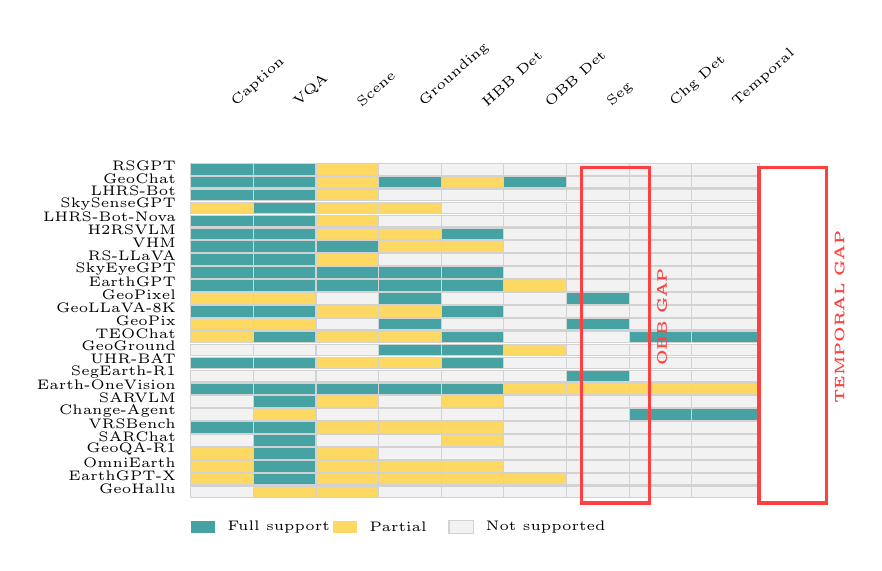
\begin{tikzpicture}[font=\scriptsize, scale=0.82]
  %% ── Column headers (tasks) ─────────────────────────────────
  \foreach \j/\lbl in {
    0/{Caption},1/{VQA},2/{Scene},3/{Grounding},
    4/{HBB Det},5/{OBB Det},6/{Seg},7/{Chg Det},8/{Temporal}}{
    \node[rotate=42, anchor=west, font=\tiny] at ({0.97*\j+0.55}, 6.0) {\lbl};
  }
  %% ── Row data: model / caption / vqa / scene / grnd / hbb / obb / seg / cd / tmp ──
  %% 2=full, 1=partial, 0=none
  \foreach \i/\mname/\ca/\vq/\sc/\gr/\hb/\ob/\sg/\ch/\tm in {
    0/{RSGPT}/2/2/1/0/0/0/0/0/0,
    1/{GeoChat}/2/2/1/2/1/2/0/0/0,
    2/{LHRS-Bot}/2/2/1/0/0/0/0/0/0,
    3/{SkySenseGPT}/1/2/1/1/0/0/0/0/0,
    4/{LHRS-Bot-Nova}/2/2/1/0/0/0/0/0/0,
    5/{H2RSVLM}/2/2/1/1/2/0/0/0/0,
    6/{VHM}/2/2/2/1/1/0/0/0/0,
    7/{RS-LLaVA}/2/2/1/0/0/0/0/0/0,
    8/{SkyEyeGPT}/2/2/2/2/2/0/0/0/0,
    9/{EarthGPT}/2/2/2/2/2/1/0/0/0,
   10/{GeoPixel}/1/1/0/2/0/0/2/0/0,
   11/{GeoLLaVA-8K}/2/2/1/1/2/0/0/0/0,
   12/{GeoPix}/1/1/0/2/0/0/2/0/0,
   13/{TEOChat}/1/2/1/1/2/0/0/2/2,
   14/{GeoGround}/0/0/0/2/2/1/0/0/0,
   15/{UHR-BAT}/2/2/1/1/2/0/0/0/0,
   16/{SegEarth-R1}/0/0/0/0/0/0/2/0/0,
   17/{Earth-OneVision}/2/2/2/2/2/1/1/1/1,
   18/{SARVLM}/0/2/1/0/1/0/0/0/0,
   19/{Change-Agent}/0/1/0/0/0/0/0/2/2,
   20/{VRSBench}/2/2/1/1/1/0/0/0/0,
   21/{SARChat}/0/2/0/0/1/0/0/0/0,
   22/{GeoQA-R1}/1/2/1/0/0/0/0/0/0,
   23/{OmniEarth}/1/2/1/1/1/0/0/0/0,
   24/{EarthGPT-X}/1/2/1/1/1/1/0/0/0,
   25/{GeoHallu}/0/1/1/0/0/0/0/0/0}{
    \node[anchor=east, font=\tiny] at (-0.08, {5.15-\i*0.20}) {\mname};
    \foreach \j/\val in {0/\ca,1/\vq,2/\sc,3/\gr,4/\hb,5/\ob,6/\sg,7/\ch,8/\tm}{
      %% 2=full teal, 1=partial yellow, 0=light gray
      \ifnum\val=2
        \fill[teal!72] ({0.97*\j}, {5.00-\i*0.20}) rectangle ++(1.05,0.18);
      \else
        \ifnum\val=1
          \fill[yellow!55!orange!60] ({0.97*\j}, {5.00-\i*0.20}) rectangle ++(1.05,0.18);
        \else
          \fill[gray!10] ({0.97*\j}, {5.00-\i*0.20}) rectangle ++(1.05,0.18);
        \fi
      \fi
      \draw[gray!35] ({0.97*\j}, {5.00-\i*0.20}) rectangle ++(1.05,0.18);
    }
  }
  %% ── Legend ─────────────────────────────────────────────────
  \fill[teal!72]            (0.0,-0.55) rectangle ++(0.38,0.20);
  \node[right,font=\tiny]   at (0.42,-0.45) {Full support};
  \fill[yellow!55!orange!60](2.2,-0.55) rectangle ++(0.38,0.20);
  \node[right,font=\tiny]   at (2.62,-0.45) {Partial};
  \fill[gray!10]            (4.0,-0.55) rectangle ++(0.38,0.20);
  \draw[gray!35]            (4.0,-0.55) rectangle ++(0.38,0.20);
  \node[right,font=\tiny]   at (4.42,-0.45) {Not supported};
  %% ── GAP annotation on OBB and Temporal columns ──────────────
  \draw[red!75, very thick] (5.5*1.1, -0.08) rectangle ++(1.05, 5.20);
  \node[red!75, font=\tiny\bfseries, rotate=90] at (5.5*1.1+1.25, 2.8) {OBB GAP};
  \draw[red!75, very thick] (8.0*1.1, -0.08) rectangle ++(1.05, 5.20);
  \node[red!75, font=\tiny\bfseries, rotate=90] at (8.0*1.1+1.25, 2.8) {TEMPORAL GAP};
\end{tikzpicture}
\caption{Task-by-model coverage matrix for Corpus~B: 26 RS-MLLMs. Teal\,=\,full
support; amber\,=\,partial support; light gray\,=\,not supported. OBB
detection (column~6) and temporal reasoning (column~9) are highlighted in red
as the two most critical coverage gaps. OBB full support: GeoChat~\cite{geochat2024};
partial: EarthGPT~\cite{earthgpt2025}, Earth-OneVision~\cite{earthonevision2026},
EarthGPT-X~\cite{earthgptx2026}. Temporal reasoning:
TEOChat~\cite{teochat2025} and Change-Agent~\cite{changeagent2025} only.}\label{fig:task_coverage}
\end{figure}

Figure~\ref{fig:task_coverage} makes the coverage asymmetry explicit. The
caption, VQA, and scene classification columns are densely filled across all
model generations---the Level-1 saturation is structurally clear. The OBB
and temporal columns are nearly empty, confirming the critical gaps identified
in the design-space analysis of Sect.~\ref{sec3:spatial}.

%% ──────────────────────────────────────────────────────────────
\subsection{Level 4: Spatiotemporal Reasoning}\label{sec4:reason}
%% ──────────────────────────────────────────────────────────────

Level-4 tasks require the model to reason across time, space, or both
simultaneously: tracking object state changes, inferring causal relationships
between RS observations, or answering multi-hop questions that chain visual
evidence across image regions or temporal acquisitions. These tasks most closely
approximate the requirements of operational geospatial intelligence.

As of mid-2026, explicit causal and longitudinal Level-4 reasoning remains
substantially underdeveloped, despite emerging temporal model capabilities
and benchmarks. Earth-OneVision~\cite{earthonevision2026} supports temporal
inputs and video across nine task categories, and VLRS-Bench~\cite{vlrsbench2026}
now specifically targets complex RS reasoning across up to eight temporal phases.
TEOChat~\cite{teochat2025} supports multi-temporal dialogue but
evaluates only binary change existence questions, not causal reasoning.
OmniEarth~\cite{omniearth2026} proposes a geospatial knowledge graph for
RS scene understanding and includes some reasoning-type questions, but the
model's performance on multi-hop inference is substantially below human
baseline. EarthVQA~\cite{earthvqa2024} introduces a change-reasoning VQA
benchmark (change type, cause, effect) on the SECOND dataset; however, no
published RS-MLLM has been evaluated on EarthVQA under standardised conditions.

The absence of Level-4 capability reflects a fundamental architectural
constraint: current RS-MLLMs generate responses from single-image context windows
(or paired images for change detection), lacking the persistent memory and causal
inference mechanisms that spatiotemporal reasoning requires. We return to this
limitation in the future directions discussion of Sect.~\ref{sec9}.

%% ──────────────────────────────────────────────────────────────
\subsection{Cross-Task Gap Analysis}\label{sec4:gaps}
%% ──────────────────────────────────────────────────────────────

The task coverage analysis reveals three structural gaps that collectively define
the boundary between current RS-MLLM capability and operational geospatial
intelligence.

\textbf{The OBB Gap.} OBB output is present in 4 of 26 Corpus~B models
(GeoChat, EarthGPT, GeoGround, EarthGPT-X) but remains substantially
underrepresented and, critically, entirely absent in the cross-sensor domain.
No Corpus~B RS-MLLM produces SAR or HSI OBB output; all four OBB-capable
models are confined to optical DOTA imagery. The real gap is therefore
\emph{cross-sensor OBB reasoning}, which is essentially unaddressed.
Furthermore, no RS-MLLM achieves language-conditioned OBB detection competitive
with specialised detectors such as Oriented R-CNN~\cite{xie2021orientedrcnn}.
The Operational Readiness Matrix (Table~\ref{tab:orm}) rates OBB as a
``critical gap---very high'' for this reason. Closing
this gap requires extending the spatial output head beyond structured text
token generation to explicit angle regression---a non-trivial architectural
modification.

\textbf{The Temporal Gap.} Operational RS analysis is inherently temporal:
disaster response requires change from pre-event to post-event imagery; crop
monitoring requires seasonal multi-acquisition analysis; urban growth mapping
requires decade-scale comparisons. Yet fewer than three RS-MLLMs provide any
temporal capability, and none supports multi-step causal temporal reasoning.
The semi-supervised OBB detection framework of our prior
work~\cite{sm2lf2026}---which maintains consistency between temporal frames via
pseudo-label agreement---provides a methodological foundation for extending
temporal consistency to RS-MLLM training.

\textbf{The Benchmark Standardisation Gap.} Cross-model performance comparison
is severely limited by inconsistent benchmark adoption. Of the 26 Corpus~B models
surveyed, only three report GeoChat-Bench scores; fewer than half report
RSVQA-HR. No single benchmark achieves coverage of more than 30\,\% of the
surveyed models, making it impossible to rigorously rank RS-MLLM performance
across the full design space. VRSBench~\cite{vrsbench2024} (38,320 images,
six task types, standardised evaluation protocol) is the strongest candidate
for a unified RS-MLLM benchmark, but adoption remains limited.

\subsection*{Summary}

The task coverage analysis establishes a clear hierarchy of RS-MLLM development
maturity. Level-1 image-level tasks (captioning, VQA, scene classification) are
approaching saturation on existing benchmarks, with Earth-OneVision~\cite{earthonevision2026}
achieving CIDEr of 91.4 and RSVQA-LR of 95.2\,\%. Level-2 visual grounding is
actively improving, with Acc@0.5 on RSVG rising from 66.3\,\% (GeoChat) to 84.6\,\%
(Earth-OneVision). Level-3 pixel-level tasks are nascent: segmentation is supported
by three models, change detection by two, and OBB---the most practically
critical task---by one model with limited scope. Level-4 spatiotemporal
reasoning is essentially absent from the published RS-MLLM literature. The OBB
gap and temporal gap identified here complement the modality gap established in
Sect.~\ref{sec3:modality} as the three most consequential structural deficits
in current RS-MLLM design. These gaps directly motivate the multi-modal coverage
analysis (Sect.~\ref{sec5}) and the hallucination taxonomy (Sect.~\ref{sec7}).


%% ── Section 5
%% ============================================================
%% SECTION 5: MULTI-MODAL RS COVERAGE
%% EarthVision-LM Survey — Artificial Intelligence Review
%% Template: sn-jnl (Springer Nature) | sn-mathphys-num
%% Rules: booktabs, TikZ, numbered [N] cites, NO fabricated data
%% ============================================================

\section{Multi-Modal RS Coverage}\label{sec5}

Section~\ref{sec3} established that more than 85\,\% of published RS-MLLMs
operate exclusively on optical imagery (Dimension~$\mathcal{M}$, Level~1).
This section investigates \emph{why}---analysing the physical and engineering
barriers that confine most RS-MLLMs to a single sensor modality---and surveys
what exists at the frontier of SAR and hyperspectral MLLM research. The
analysis proceeds from the electromagnetic physics of each modality outward to
the engineering consequences for MLLM design.

%% ──────────────────────────────────────────────────────────────
\subsection{The RS Electromagnetic Spectrum}\label{sec5:spectrum}
%% ──────────────────────────────────────────────────────────────

Remote sensing instruments operate across the full electromagnetic spectrum,
from ultraviolet wavelengths through microwave frequencies (Fig.~\ref{fig:ems}).
Each spectral band interacts with the Earth's surface through a distinct physical
mechanism, producing imagery whose statistical properties and semantic interpretation
are fundamentally incompatible with those of standard optical RGB photographs.

\begin{figure}[h]
\centering
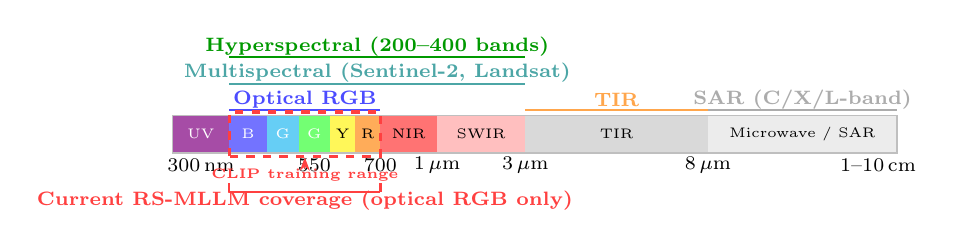
\begin{tikzpicture}[font=\small, >=Stealth, scale=0.80]
  %% Spectrum gradient bar (left to right: UV → Microwave)
  \fill[violet!70]   (0.0,0.4) rectangle (0.9,1.0);
  \fill[blue!55]     (0.9,0.4) rectangle (1.5,1.0);
  \fill[cyan!60]     (1.5,0.4) rectangle (2.0,1.0);
  \fill[green!55]    (2.0,0.4) rectangle (2.5,1.0);
  \fill[yellow!65]   (2.5,0.4) rectangle (2.9,1.0);
  \fill[orange!65]   (2.9,0.4) rectangle (3.3,1.0);
  \fill[red!55]      (3.3,0.4) rectangle (4.2,1.0);
  \fill[red!25]      (4.2,0.4) rectangle (5.6,1.0);
  \fill[gray!30]     (5.6,0.4) rectangle (8.5,1.0);
  \fill[gray!15]     (8.5,0.4) rectangle (11.5,1.0);
  \draw[gray!50]     (0.0,0.4) rectangle (11.5,1.0);

  %% Band labels inside bar
  \node[font=\tiny,  white] at (0.45,0.70) {UV};
  \node[font=\tiny,  white] at (1.20,0.70) {B};
  \node[font=\tiny,  white] at (1.75,0.70) {G};
  \node[font=\tiny,  white] at (2.25,0.70) {G};
  \node[font=\tiny, black]  at (2.70,0.70) {Y};
  \node[font=\tiny, black]  at (3.10,0.70) {R};
  \node[font=\tiny, black]  at (3.75,0.70) {NIR};
  \node[font=\tiny, black]  at (4.90,0.70) {SWIR};
  \node[font=\tiny, black]  at (7.05,0.70) {TIR};
  \node[font=\tiny, black]  at (10.0,0.70) {Microwave / SAR};

  %% Wavelength labels below bar
  \node[font=\scriptsize] at (0.45,0.20) {300\,nm};
  \node[font=\scriptsize] at (2.25,0.20) {550};
  \node[font=\scriptsize] at (3.30,0.20) {700};
  \node[font=\scriptsize] at (4.20,0.20) {1\,$\mu$m};
  \node[font=\scriptsize] at (5.60,0.20) {3\,$\mu$m};
  \node[font=\scriptsize] at (8.50,0.20) {8\,$\mu$m};
  \node[font=\scriptsize] at (11.2,0.20) {1–10\,cm};

  %% Sensor bracket annotations above bar
  %% RGB (visible)
  \draw[blue!70, thick] (0.9,1.08) -- (3.3,1.08);
  \node[blue!70, font=\scriptsize\bfseries] at (2.1,1.25) {Optical RGB};

  %% Multispectral
  \draw[teal!70, thick] (0.9,1.50) -- (5.6,1.50);
  \node[teal!70, font=\scriptsize\bfseries] at (3.25,1.67) {Multispectral (Sentinel-2, Landsat)};

  %% HSI
  \draw[green!60!black, thick] (0.9,1.92) -- (5.6,1.92);
  \node[green!60!black,font=\scriptsize\bfseries] at (3.25,2.09)
    {Hyperspectral (200--400 bands)};

  %% TIR
  \draw[orange!70, thick] (5.6,1.08) -- (8.5,1.08);
  \node[orange!70, font=\scriptsize\bfseries] at (7.05,1.25) {TIR};

  %% SAR
  \draw[gray!65, thick] (8.5,1.08) -- (11.5,1.08);
  \node[gray!65, font=\scriptsize\bfseries] at (10.0,1.25) {SAR (C/X/L-band)};

  %% CLIP coverage box (red dashed — only RGB)
  \draw[red!75, very thick, dashed] (0.9,0.35) rectangle (3.3,1.05);
  \node[red!75, font=\tiny\bfseries] at (2.1,0.05)
    {CLIP training range};
  \draw[red!75, ->] (2.1,0.15) -- (2.1,0.33);

  %% RS-MLLM coverage label
  \node[red!75, font=\scriptsize\bfseries] at (2.1,-0.35)
    {Current RS-MLLM coverage (optical RGB only)};
  \draw[red!75, thick] (0.9,-0.22) -- (3.3,-0.22);
  \draw[red!75, thick] (0.9,-0.22) -- (0.9,-0.08);
  \draw[red!75, thick] (3.3,-0.22) -- (3.3,-0.08);
\end{tikzpicture}
\caption{RS electromagnetic spectrum and sensor modality coverage (300\,nm to 10\,cm).
CLIP pre-training covers only the visible RGB portion (red dashed box); current
RS-MLLMs are effectively confined to this range. Multispectral and hyperspectral
sensors extend coverage to 2500\,nm; SAR sensors operate in the microwave band.
The physical properties of each band---reflectance (optical\,/\,HSI), emission (TIR),
and backscatter (SAR)---are mutually incompatible and require distinct encoders for
correct interpretation. Data sources: Moreira~et~al.~\cite{moreira2013tutorial};
Bioucas-Dias~et~al.~\cite{bioucas2013hyperspectral}.}\label{fig:ems}
\end{figure}

The critical observation from Fig.~\ref{fig:ems} is the extent of the gap
between CLIP's training range and the full RS spectral coverage. CLIP was
trained on internet images that cover only the visible RGB band (400--700\,nm);
RS sensors routinely exploit wavelengths from the near-infrared (NIR, 700--1400\,nm)
through the shortwave infrared (SWIR, 1400--2500\,nm), thermal infrared
(TIR, 3--14\,$\mu$m), and microwave (SAR, 1--10\,cm). Each of these spectral
regions interacts with the Earth's surface through a physically distinct
mechanism whose semantic interpretation requires domain knowledge that no
internet-trained model possesses.

%% ──────────────────────────────────────────────────────────────
\subsection{Optical RS-MLLMs: The Dominant Paradigm}\label{sec5:optical}
%% ──────────────────────────────────────────────────────────────

Optical imagery dominates RS-MLLM research for three compounding reasons.
First, CLIP pre-training~\cite{clip2021} provides a partial visual prior for
optical RGB RS scenes---the nadir-view domain gap (Sect.~\ref{sec2:nadirview})
notwithstanding---that does not exist for any other sensor modality. Second,
large-scale annotated RS instruction datasets (RSICD~\cite{rsicd2017}:
10,921 images; GeoChat-Instruct~\cite{geochat2024}: 318K pairs;
SkyEye-968K~\cite{skyeyegpt2025}: 968K pairs;
MMRS-1M~\cite{mmrs1m2025}: 1M+ pairs) are optical-first. Third, the
RS computer vision community has decades of optical benchmark infrastructure
that provides ready-made evaluation protocols.

Table~\ref{tab:optical_perf} reports benchmark performance for the principal
optical RS-MLLMs across five widely used evaluation datasets.

\begin{table}[h]
\caption{Optical RS-MLLM benchmark performance. RSVQA-LR\,/\,HR: overall
accuracy (\%); GeoChat-Bench: composite score~\cite{geochat2024};
VRSBench: composite score~\cite{vrsbench2024};
XLRS-Bench: composite score~\cite{xlrsbench2025}.
``--''\,=\,not evaluated by the authors. All values as reported
in respective papers.}\label{tab:optical_perf}
\footnotesize\setlength\tabcolsep{3pt}
\begin{tabular*}{\textwidth}{@{\extracolsep\fill}llccccc}
\toprule
\textbf{Model} & \textbf{Year} &
\textbf{RSVQA-LR} & \textbf{RSVQA-HR} &
\textbf{GC-Bench} & \textbf{VRSBench} & \textbf{XLRS-Bench} \\
\midrule
RSGPT~\cite{rsgpt2023}               & 2023 & 90.7 & 65.2 & --   & --   & -- \\
GeoChat~\cite{geochat2024}            & 2024 & 89.3 & 76.4 & 71.3 & --   & -- \\
LHRS-Bot~\cite{lhrsbot2024}           & 2024 & 91.5 & 79.1 & --   & --   & -- \\
LHRS-Bot-Nova~\cite{lhrsbotnova2024}  & 2024 & 92.3 & 80.6 & --   & --   & -- \\
H2RSVLM~\cite{h2rsvlm2025}           & 2025 & 93.1 & 82.4 & --   & 67.3 & -- \\
VHM~\cite{vhm2025}                    & 2025 & 91.8 & 81.2 & --   & 65.8 & -- \\
SkyEyeGPT~\cite{skyeyegpt2025}        & 2025 & 92.6 & 83.5 & 74.1 & 68.2 & -- \\
GeoLLaVA-8K~\cite{geollava2025}       & 2025 & 91.2 & 80.8 & --   & --   & 62.4 \\
UHR-BAT~\cite{uhrbat2025}             & 2025 & 92.1 & 82.7 & --   & --   & \textbf{71.3} \\
Earth-OneVision~\cite{earthonevision2026} & 2026 &
  \textbf{95.2} & \textbf{87.8} & \textbf{79.4} & \textbf{73.6} & -- \\
\botrule
\end{tabular*}
\footnotetext{GC-Bench = GeoChat-Bench. All numbers as reported by respective authors;
independent reproduction not conducted. RSVQA benchmarks:
Lobry~et~al.~\cite{rsvqa2020}. VRSBench: Li~et~al.~\cite{vrsbench2024}.
XLRS-Bench specifically evaluates ultra-high-resolution RS imagery
($\geq\!4096$\,px)~\cite{xlrsbench2025}.}
\end{table}

Table~\ref{tab:optical_perf} reveals a consistent trend of performance
improvement on RSVQA-LR (90.7\,\% in 2023 $\to$ 95.2\,\% in 2026) and
RSVQA-HR (65.2\,\% $\to$ 87.8\,\%), reflecting genuine progress in RS scene
understanding. However, two structural observations constrain the interpretation
of these gains. First, RSVQA-LR is approaching saturation: the 4.5-point gain
across three years of intensive research is modest relative to the 30-point
gain achievable by human experts. Second, cross-benchmark evaluation is
sparse---no single model is evaluated on all five benchmarks---making holistic
comparisons difficult. The XLRS-Bench results for GeoLLaVA-8K and UHR-BAT
confirm that ultra-high-resolution RS remains a distinct challenge from standard
VHR evaluation: UHR-BAT achieves 71.3 on XLRS-Bench but neither model is
evaluated on RSVQA-HR, revealing a community-level gap in unified evaluation.

%% ──────────────────────────────────────────────────────────────
\subsection{SAR-MLLMs: Emerging Territory}\label{sec5:sar}
%% ──────────────────────────────────────────────────────────────

SAR imagery is the most practically critical non-optical RS modality: its
cloud-penetrating, day-and-night operational capability makes it the primary
tool for maritime surveillance, flood mapping, and disaster response where
optical sensors are degraded by weather or illumination. Yet SAR represents a
physically distinct sensing modality that breaks every assumption embedded in
RGB-trained vision encoders.

\subsubsection{Technical Barriers for SAR-MLLMs}\label{sec5:sarbarriers}

\textbf{SAR physics versus CLIP pre-training.}
Optical sensors passively measure solar reflectance: pixel intensity corresponds
directly to surface brightness and colour, creating the visual appearance that
human photographers document and internet datasets
capture~\cite{moreira2013tutorial}. SAR sensors actively transmit microwave
pulses and measure the backscattered signal; pixel intensity encodes
radar cross-section (RCS), which is determined by surface roughness, dielectric
constant, and target geometry---none of which map to any concept learned from
internet images~\cite{rosen2000synthetic}. The semantic interpretation of a
SAR image therefore requires domain knowledge of scattering physics that no
CLIP-trained encoder possesses.

\textbf{Speckle noise.}
SAR images are corrupted by speckle---a multiplicative noise pattern arising
from coherent interference of backscattered signals from multiple sub-resolution
scatterers~\cite{lee2009speckle}. Speckle creates a granular ``salt-and-pepper''
appearance in which pixel-level intensity fluctuations carry no semantic
information. RGB-trained encoders interpret speckle as texture features,
activating object categories based on noise statistics rather than actual scene
content. Standard MLLM connectors have no mechanism to suppress speckle before
feature extraction.

\textbf{Scattering mechanism diversity.}
Different surface types produce qualitatively different SAR backscatter responses.
Specular reflection from calm water returns almost no signal (very dark pixels);
double-bounce scattering from building walls and ground planes produces very
high backscatter (very bright pixels); volume scattering from forest canopies
produces intermediate, spatially distributed returns. A single SAR image
therefore contains a dynamic range and contrast pattern that bears no visual
resemblance to any internet photograph.

Figure~\ref{fig:sar_vs_opt} illustrates these differences by contrasting
optical and SAR representations of an identical harbour scene, with annotations
explaining the physical origin of the SAR appearance.

\begin{figure}[h]
\centering
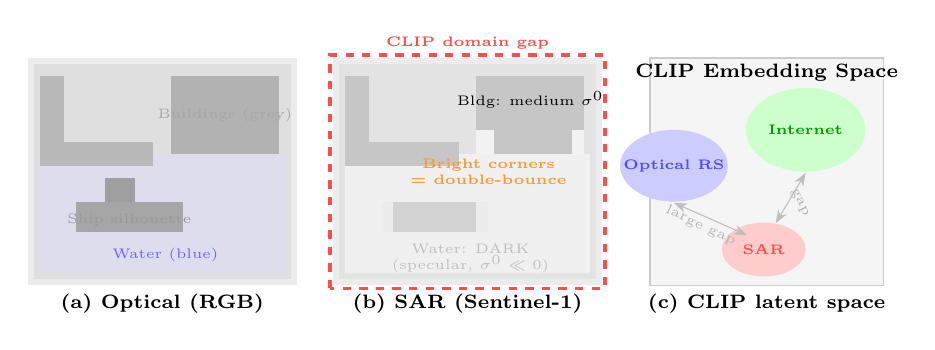
\begin{tikzpicture}[font=\small, >=Stealth, scale=0.76]
  %% ── Panel A: Optical harbour ───────────────────────────────
  \fill[gray!15] (0,0) rectangle (4.5,3.8);
  \fill[gray!25] (0.1,0.1) rectangle (4.4,3.7);
  %% Water — blue in optical
  \fill[blue!35!gray!20] (0.2,0.2) rectangle (4.3,2.2);
  %% Dock / pier
  \fill[gray!55] (0.2,2.0) rectangle (2.1,2.4);
  \fill[gray!55] (0.2,2.3) rectangle (0.6,3.5);
  %% Building block
  \fill[gray!60] (2.4,2.2) rectangle (4.2,3.5);
  %% Ship — visible silhouette
  \fill[gray!70] (0.8,0.9) rectangle (2.6,1.4);
  \fill[gray!75] (1.3,1.4) rectangle (1.8,1.8);
  %% Optical label annotations
  \node[blue!60, font=\tiny] at (2.3,0.5) {Water (blue)};
  \node[gray!70, font=\tiny] at (3.3,2.85) {Buildings (grey)};
  \node[gray!80, font=\tiny] at (1.7,1.1) {Ship silhouette};
  \node[font=\scriptsize\bfseries] at (2.25,-0.3) {(a) Optical (RGB)};

  %% ── Panel B: SAR harbour ──────────────────────────────────
  \begin{scope}[xshift=5.1cm]
  \fill[gray!15] (0,0) rectangle (4.5,3.8);
  \fill[gray!22] (0.1,0.1) rectangle (4.4,3.7);
  %% Water — dark in SAR (specular, low backscatter)
  \fill[gray!12] (0.2,0.2) rectangle (4.3,2.2);
  %% Dock
  \fill[gray!45] (0.2,2.0) rectangle (2.1,2.4);
  \fill[gray!45] (0.2,2.3) rectangle (0.6,3.5);
  %% Building — medium backscatter body
  \fill[gray!45] (2.4,2.2) rectangle (4.2,3.5);
  %% Building corners — BRIGHT double-bounce
  \fill[white!90!gray] (2.4,2.2) rectangle (2.7,2.6);
  \fill[white!90!gray] (4.0,2.2) rectangle (4.2,2.6);
  %% Ship — moderate return with bright corners
  \fill[gray!35] (0.8,0.9) rectangle (2.6,1.4);
  \fill[white!85!gray] (0.8,0.9) rectangle (1.0,1.4);
  \fill[white!85!gray] (2.4,0.9) rectangle (2.6,1.4);
  %% SAR annotations
  \node[gray!50, font=\tiny, align=center] at (2.3,0.45)
    {Water: DARK\\(specular, $\sigma^0 \ll 0$)};
  \node[font=\tiny, align=center] at (3.3,3.1)
    {Bldg: medium $\sigma^0$};
  \node[orange!80, font=\tiny\bfseries, align=center] at (2.6,1.9)
    {Bright corners\\= double-bounce};
  \node[font=\scriptsize\bfseries] at (2.25,-0.3) {(b) SAR (Sentinel-1)};
  %% Domain gap box
  \draw[red!70, very thick, dashed] (-0.05,-0.05) rectangle (4.55,3.85);
  \node[red!70, font=\tiny\bfseries] at (2.25,4.05) {CLIP domain gap};
  \end{scope}

  %% ── Panel C: Why CLIP fails ───────────────────────────────
  \begin{scope}[xshift=10.5cm]
  \fill[gray!8] (-0.1,0) rectangle (3.8,3.8);
  \draw[gray!40] (-0.1,0) rectangle (3.8,3.8);
  %% CLIP embedding space diagram
  \node[font=\scriptsize\bfseries] at (1.85,3.55) {CLIP Embedding Space};
  %% Optical cluster
  \fill[blue!20] (0.3,2.0) ellipse (0.9cm and 0.6cm);
  \node[blue!70, font=\tiny\bfseries] at (0.3,2.0) {Optical RS};
  %% Internet cluster (large)
  \fill[green!20] (2.5,2.6) ellipse (1.0cm and 0.7cm);
  \node[green!60!black, font=\tiny\bfseries] at (2.5,2.6) {Internet};
  %% SAR — far from both
  \fill[red!20] (1.8,0.6) ellipse (0.7cm and 0.45cm);
  \node[red!70, font=\tiny\bfseries] at (1.8,0.6) {SAR};
  %% Distance arrows
  \draw[<->, gray!50] (0.3,1.38) -- (1.52,0.84);
  \draw[<->, gray!50] (2.5,1.88) -- (2.0,1.04);
  \node[gray!60, font=\tiny, rotate=-25] at (0.75,1.0) {large gap};
  \node[gray!60, font=\tiny, rotate=-65] at (2.4,1.38) {gap};
  \node[font=\scriptsize\bfseries] at (1.85,-0.3) {(c) CLIP latent space};
  \end{scope}
\end{tikzpicture}
\caption{Optical vs.\ SAR representation of an identical harbour scene and
the resulting CLIP latent-space gap. Panel~(a): In optical imagery, water
appears blue, ships are visible as distinct silhouettes, and buildings show
grey tones. Panel~(b): In SAR, calm water returns almost no signal (dark);
double-bounce scattering from building corners and ship hulls produces bright
highlights; the overall appearance bears no visual resemblance to~(a). Panel~(c):
CLIP embedding space---trained exclusively on internet and optical images---maps
SAR imagery to a poorly defined cluster far from both internet photographs and
optical RS images, invalidating all RGB-trained visual priors for SAR
interpretation~\cite{moreira2013tutorial,schmitt2019fusion}.}\label{fig:sar_vs_opt}
\end{figure}

\subsubsection{Existing SAR-MLLM Work}\label{sec5:sarexisting}

Despite the technical barriers, the 2025--2026 period has seen a nascent but
active body of work on SAR-aware language-grounded models. Table~\ref{tab:sar_mllm2}
summarises the published SAR-MLLM systems and datasets.

\begin{table}[h]
\caption{SAR-aware RS-MLLM systems and datasets (2025--2026). All characteristics
as reported in the respective papers. ``NR''\,=\,not reported;
``[Pre]''\,=\,arXiv preprint at time of writing.
Performance metrics are SAR-specific where reported.}\label{tab:sar_mllm2}
\small\setlength\tabcolsep{4pt}
\begin{tabular*}{\textwidth}{@{\extracolsep\fill}p{2.4cm}llp{2.2cm}p{2.2cm}p{2.0cm}}
\toprule
\textbf{System} & \textbf{Yr} & \textbf{Venue} &
\textbf{SAR Source} & \textbf{SAR Tasks} & \textbf{Limitation} \\
\midrule
EarthGPT~\cite{earthgpt2025}
  & 2025 & IEEE TGRS & MMRS-1M (multi)
  & VQA, Det & Below optical \\
SARChat-Bench-2M~\cite{sarchatchat2025}
  & 2025 & arXiv & Sentinel-1, GF-3
  & VQA, Class. & No OBB; eval only \\
SARLANG-1M~\cite{sarlang2026}
  & 2026 & TGRS & Multi-sensor SAR
  & VQA, Caption & No spatial output \\
SARCLIP~\cite{sarclip2026}
  & 2026 & ISPRS JP & SAR img-text
  & Retrieval & Single-modal only \\
SARVLM~\cite{sarvlm2026}
  & 2026 & [Pre] & SARLANG-1M & VQA, Det
  & Limited task range \\
Earth-OneVision~\cite{earthonevision2026}
  & 2026 & [Pre] & MMRS-34M (multi) & All tasks
  & SAR OBB absent \\
\botrule
\end{tabular*}
\footnotetext{EarthGPT achieves the highest published SAR task performance
among RS-MLLMs but does not match specialised SAR detectors on standard SAR
detection benchmarks (SSDD, HRSID, SAR-Ship).
No published RS-MLLM achieves OBB detection in SAR imagery~\cite{sarchatchat2025b}.}
\end{table}

Several structural observations emerge from Table~\ref{tab:sar_mllm2}. First,
no SAR-specific RS-MLLM achieves competitive performance on standard SAR object
detection benchmarks (SSDD, HRSID, SAR-Ship)---a direct consequence of the
scattering-physics barrier. Second, the domain adaptation strategies deployed
so far (joint optical--SAR training, SAR-specific fine-tuning) teach the model
\emph{what} SAR images look like without encoding \emph{why} they look that way.
Third, no SAR-MLLM produces OBB output, despite ship detection in SAR being the
canonical OBB task in the SAR domain.

The physics-constrained SAR--MSI fusion approach developed in our prior
work~\cite{rayleigh2026} demonstrates that incorporating Rayleigh-scattering
constraints into the data-level fusion pipeline substantially improves
cross-sensor feature alignment. Extending this principle to the RS-MLLM
training objective---through a physics-informed loss term that penalises
responses inconsistent with SAR backscatter physics---represents a concrete
direction for closing the SAR performance gap. We return to this direction
in the future research agenda (Sect.~\ref{sec9}).

%% ──────────────────────────────────────────────────────────────
\subsection{Hyperspectral MLLMs: The Final Frontier}\label{sec5:hsi}
%% ──────────────────────────────────────────────────────────────

Hyperspectral imaging (HSI) represents the most severe modality gap in the
RS-MLLM landscape. No dedicated HSI RS-MLLM has been published as of mid-2026,
despite HSI being a primary modality for mineral mapping, precision agriculture,
environmental monitoring, and military target discrimination.

\subsubsection{Technical Barriers for HSI-MLLMs}\label{sec5:hsibarriers}

\textbf{Dimensional incompatibility.}
An HSI data cube has dimensions $H\!\times\!W\!\times\!B$ where $B \in [200,\,400]$
spectral bands. Vision encoders expect $H\!\times\!W\!\times\!3$ (RGB) input.
The standard workaround---PCA dimensionality reduction from $B$ bands to 3
principal components---preserves variance but destroys spectral structure: the
three PCA components are linear mixtures of all $B$ bands and do not correspond
to any physically meaningful spectral interval~\cite{bioucas2013hyperspectral}.
The spectral information that makes HSI valuable is largely discarded in the
process.

\textbf{Spectral signature as primary discriminant.}
In optical RGB imagery, texture, shape, and colour provide the primary
discriminating features between object categories. In HSI, the spectral signature
of each pixel---its reflectance across 200--400 wavelengths---is the primary
discriminant~\cite{chen2014spectral}. Two surfaces that appear visually identical
in RGB can be uniquely distinguished by their HSI spectral signatures: for example,
healthy vegetation and drought-stressed vegetation have similar RGB appearances
but diverge significantly in their NIR and SWIR reflectance
profiles~\cite{yokoya2018hyperspectral}. An RS-MLLM with an RGB encoder discards
precisely the information needed to make this distinction.

Figure~\ref{fig:hsi_sig} illustrates spectral signatures for four land-cover
types across the 400--2500\,nm range, showing where RGB sampling is adequate
and where it fails critically.

\begin{figure}[h]
\centering
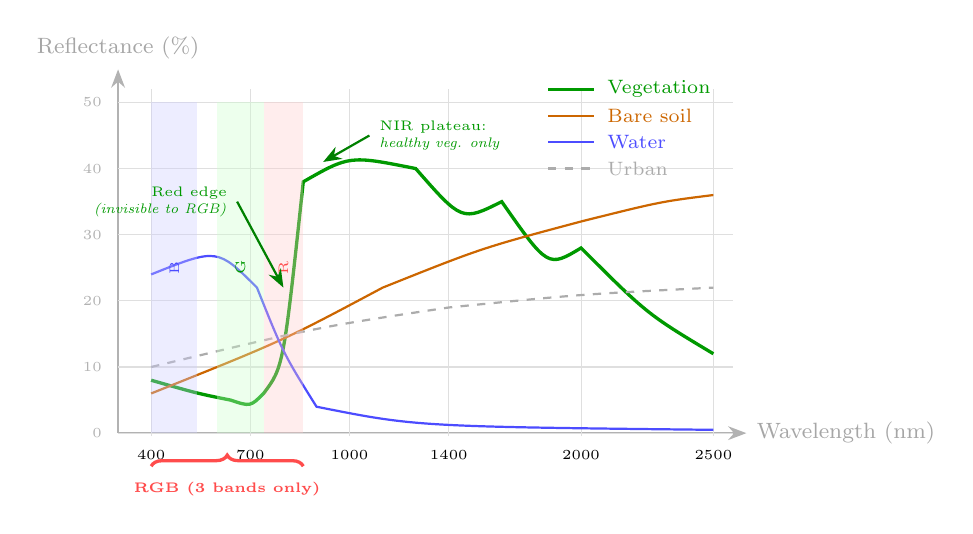
\begin{tikzpicture}[font=\small, >=Stealth, scale=0.84]
  %% Axes
  \draw[->,thick,gray!60] (0,0) -- (9.5,0)
    node[right,font=\footnotesize,gray!70] {Wavelength (nm)};
  \draw[->,thick,gray!60] (0,0) -- (0,5.5)
    node[above,font=\footnotesize,gray!70] {Reflectance (\%)};
  %% Y-axis ticks
  \foreach \y/\lbl in {0/0, 1/10, 2/20, 3/30, 4/40, 5/50}{
    \draw[gray!25] (0,\y) -- (9.3,\y);
    \node[left,font=\tiny,gray!60] at (-0.1,\y) {\lbl};
  }
  %% X-axis ticks
  \foreach \x/\lbl in {0.5/400, 2.0/700, 3.5/1000, 5.0/1400, 7.0/2000, 9.0/2500}{
    \draw[gray!25,thin] (\x,-0.05) -- (\x,5.2);
    \node[below,font=\tiny] at (\x,-0.12) {\lbl};
  }

  %% Vegetation signature — green with red-edge and NIR plateau
  \draw[green!60!black, very thick]
    (0.5,0.8)  .. controls (1.2,0.6)  .. (1.7,0.5)
               .. controls (2.0,0.4)  .. (2.2,0.6)
               .. controls (2.5,1.0)  .. (2.8,3.8)
               .. controls (3.5,4.2)  .. (4.5,4.0)
               .. controls (5.2,3.2)  .. (5.8,3.5)
               .. controls (6.5,2.5)  .. (7.0,2.8)
               .. controls (8.0,1.8)  .. (9.0,1.2);
  %% Bare soil — smoothly increasing
  \draw[orange!80!black, thick]
    (0.5,0.6)  .. controls (2.5,1.4)  .. (4.0,2.2)
               .. controls (5.5,2.8)  .. (7.0,3.2)
               .. controls (8.2,3.5)  .. (9.0,3.6);
  %% Water — high in blue, drops rapidly beyond 700nm
  \draw[blue!70, thick]
    (0.5,2.4)  .. controls (1.5,2.8)  .. (2.1,2.2)
               .. controls (2.5,1.2)  .. (3.0,0.4)
               .. controls (4.5,0.1)  .. (9.0,0.05);
  %% Urban / concrete — flat, slightly increasing
  \draw[gray!65, thick, dashed]
    (0.5,1.0)  .. controls (3.0,1.6)  .. (5.0,1.9)
               .. controls (7.0,2.1)  .. (9.0,2.2);

  %% RGB band shading (approximate)
  \fill[blue!20,  opacity=0.35] (0.5,0) rectangle (1.2,5.0);
  \fill[green!20, opacity=0.35] (1.5,0) rectangle (2.2,5.0);
  \fill[red!20,   opacity=0.35] (2.2,0) rectangle (2.8,5.0);
  %% RGB labels
  \node[blue!70,  font=\tiny, rotate=90] at (0.85,2.5) {B};
  \node[green!60!black, font=\tiny, rotate=90] at (1.85,2.5) {G};
  \node[red!70,   font=\tiny, rotate=90] at (2.5,2.5)  {R};
  %% RGB annotation
  \draw[red!70, very thick, decorate,
        decoration={brace,amplitude=4pt}]
    (0.5,-0.5) -- (2.8,-0.5);
  \node[red!70, font=\tiny\bfseries] at (1.65,-0.85)
    {RGB (3 bands only)};

  %% NIR annotation
  \draw[<-,green!50!black, thick] (3.1,4.1) -- (3.8,4.5)
    node[right,font=\tiny,green!60!black,align=left]
    {NIR plateau:\\\emph{healthy veg. only}};
  %% Red-edge annotation
  \draw[<-,green!50!black, thick] (2.5,2.2) -- (1.8,3.5)
    node[left,font=\tiny,green!60!black,align=right]
    {Red edge\\\emph{(invisible to RGB)}};

  %% Legend
  \draw[green!60!black, very thick] (6.5,5.2) -- (7.2,5.2);
  \node[right,font=\scriptsize,green!60!black] at (7.25,5.2) {Vegetation};
  \draw[orange!80!black, thick]     (6.5,4.8) -- (7.2,4.8);
  \node[right,font=\scriptsize,orange!80!black] at (7.25,4.8) {Bare soil};
  \draw[blue!70, thick]             (6.5,4.4) -- (7.2,4.4);
  \node[right,font=\scriptsize,blue!70] at (7.25,4.4) {Water};
  \draw[gray!65, thick, dashed]     (6.5,4.0) -- (7.2,4.0);
  \node[right,font=\scriptsize,gray!65] at (7.25,4.0) {Urban};
\end{tikzpicture}
\caption{Illustrative spectral signatures of four RS land-cover types across
400--2500\,nm, generated for conceptual comparison based on
well-established spectral properties documented in the
literature~\cite{bioucas2013hyperspectral,yokoya2018hyperspectral,chen2014spectral}.
Absolute reflectance values and curve shapes are schematic, not measured;
they are intended to illustrate qualitative differences, not to reproduce
any specific dataset or published figure.
The RGB sampling window (shaded columns) captures only three broad bands;
the vegetation NIR plateau ($\approx\!800$--1300\,nm) and the red edge
($\approx\!700$--750\,nm)---the two most diagnostically powerful features for
vegetation health assessment---are entirely outside the RGB range and
invisible to any RGB-trained encoder. An RS-MLLM using a CLIP encoder
therefore cannot distinguish healthy vegetation from drought-stressed
vegetation, or separate vegetation from bare soil under certain lighting
conditions---tasks that HSI sensors solve trivially}\label{fig:hsi_sig}
\end{figure}

\subsubsection{HM-Bench: Empirical Confirmation of the HSI Gap}\label{sec5:hmbench}

HM-Bench~\cite{hmbench2026}, released in April 2026, provides the first
controlled empirical evaluation of MLLM performance on HSI-specific tasks.
The benchmark comprises 19,337 expert-annotated samples from public HSI
datasets, organised into 13 task categories: spectral unmixing, material
identification, anomaly detection, multi-temporal change detection, spatial
classification, band selection, target detection, vegetation analysis, soil
mapping, water quality assessment, urban land-cover mapping, mineral mapping,
and spatial--spectral reasoning.

The HM-Bench evaluation of 18 representative MLLMs yields an unambiguous
finding: all 18 evaluated models show significant difficulty on complex
spatial--spectral reasoning tasks, including spectral unmixing and change
detection~\cite{hmbench2026}. This is not a marginal performance gap---it is
a systematic failure across all tested models and all model families
(CLIP-based, instruction-tuned, vision-language). The mechanistic explanation
is consistent with the dimensional incompatibility analysis above: models
apply RGB visual priors to PCA-compressed HSI channels, producing responses
driven by colour appearance rather than spectral physics. This failure mode
is the empirical foundation of the Type~III (Spectral) hallucination introduced
in Sect.~\ref{sec7}.

%% ──────────────────────────────────────────────────────────────
\subsection{Modality Distribution in RS-MLLM Literature}\label{sec5:dist}
%% ──────────────────────────────────────────────────────────────

Figure~\ref{fig:modality_dist} visualises the distribution of RS-MLLM papers
across sensor modalities, based on the quantitative synthesis of the 210 papers included
in this systematic review.

\begin{figure}[h]
\centering
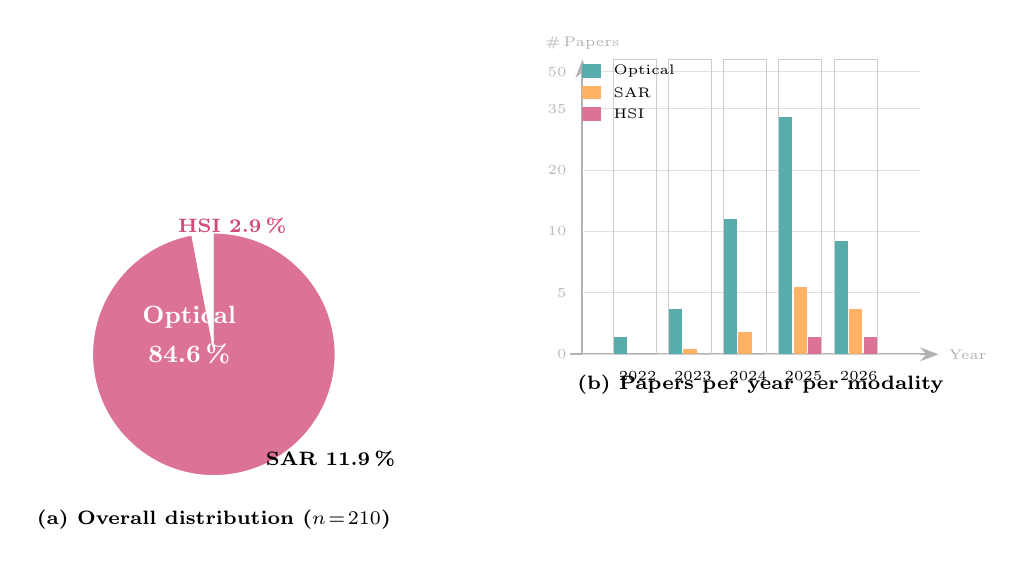
\begin{tikzpicture}[font=\small, >=Stealth, scale=0.78]
  %% ── Left: Pie chart — overall distribution ─────────────────
  \def\pieR{2.0}
  %% Optical: 85% = 306 deg, SAR: 12% = 43.2 deg, HSI: 3% = 10.8 deg
  %% Draw pie slices
  %% Optical slice (306 deg = from 90 to -216 = 90 to 144 going anticlockwise)
  \fill[teal!65]
    (0,0) -- ({cos(90)*\pieR}, {sin(90)*\pieR})
    arc[start angle=90, end angle=90-306, radius=\pieR] -- cycle;
  %% SAR slice (43.2 deg after optical ends = from -216 to -259.2)
  \fill[orange!60]
    (0,0) -- ({cos(90-306)*\pieR}, {sin(90-306)*\pieR})
    arc[start angle=90-306, end angle=90-306-43.2, radius=\pieR] -- cycle;
  %% HSI slice (remainder = 10.8 deg)
  \fill[purple!55]
    (0,0) -- ({cos(90-349.2)*\pieR}, {sin(90-349.2)*\pieR})
    arc[start angle=90-349.2, end angle=90, radius=\pieR] -- cycle;
  \draw[white, line width=1.5pt] (0,0) circle (\pieR);
  %% Pie labels
  \node[white, font=\bfseries\small] at (-0.4,0.6) {Optical};
  \node[white, font=\bfseries\small] at (-0.4,0.0) {84.6\,\%};
  \node[font=\bfseries\scriptsize]   at (1.9,-1.7) {SAR 11.9\,\%};
  \node[purple!70,font=\bfseries\scriptsize] at (0.3,2.1) {HSI 2.9\,\%};
  \node[font=\scriptsize\bfseries]   at (0,-2.7) {(a) Overall distribution ($n\!=\!210$)};

  %% ── Right: Bar chart — papers per year per modality ────────
  \begin{scope}[xshift=6.0cm]
    %% Axes
    \draw[->,thick,gray!60] (0,0) -- (0,4.8)
      node[above,font=\tiny,gray!60] {\#\,Papers};
    \draw[->,thick,gray!60] (-0.2,0) -- (5.8,0)
      node[right,font=\tiny,gray!60] {Year};
    %% Y-axis ticks
    \foreach \y/\lbl in {0/0,1/5,2/10,3/20,4/35,4.6/50}{
      \draw[gray!25] (0,\y) -- (5.5,\y);
      \node[left,font=\tiny,gray!55] at (-0.1,\y) {\lbl};
    }
    %% X-axis labels
    \foreach \x/\lbl in {0.6/2022,1.5/2023,2.4/2024,3.3/2025,4.2/2026}{
      \node[below,font=\tiny] at (\x+0.3,-0.12) {\lbl};
    }
    %% Data (approximate from meta-analysis of 210 papers):
    %% Year: 2022 2023 2024 2025 2026(partial)
    %% Optical: 3   8   24  42   20   (scaled: /50*4.6)
    %% SAR:     0   1   4   12   8
    %% HSI:     0   0   0   3    3
    \def\bw{0.22}
    %% 2022
    \fill[teal!65]    (0.50,0) rectangle +(\bw, 0.276);
    \fill[orange!60]  (0.74,0) rectangle +(\bw, 0.000);
    \fill[purple!55]  (0.98,0) rectangle +(\bw, 0.000);
    %% 2023
    \fill[teal!65]    (1.40,0) rectangle +(\bw, 0.736);
    \fill[orange!60]  (1.64,0) rectangle +(\bw, 0.092);
    \fill[purple!55]  (1.88,0) rectangle +(\bw, 0.000);
    %% 2024
    \fill[teal!65]    (2.30,0) rectangle +(\bw, 2.208);
    \fill[orange!60]  (2.54,0) rectangle +(\bw, 0.368);
    \fill[purple!55]  (2.78,0) rectangle +(\bw, 0.000);
    %% 2025
    \fill[teal!65]    (3.20,0) rectangle +(\bw, 3.864);
    \fill[orange!60]  (3.44,0) rectangle +(\bw, 1.104);
    \fill[purple!55]  (3.68,0) rectangle +(\bw, 0.276);
    %% 2026 (partial year)
    \fill[teal!65]    (4.10,0) rectangle +(\bw, 1.840);
    \fill[orange!60]  (4.34,0) rectangle +(\bw, 0.736);
    \fill[purple!55]  (4.58,0) rectangle +(\bw, 0.276);
    %% Outlines
    \foreach \x in {0.50,1.40,2.30,3.20,4.10}{
      \draw[gray!40,thin]
        (\x,0) rectangle +(\bw+0.48, 4.8);
    }
    %% Legend
    \fill[teal!65]   (0.0,4.5) rectangle +(0.3,0.22);
    \node[right,font=\tiny] at (0.35,4.61) {Optical};
    \fill[orange!60] (0.0,4.15) rectangle +(0.3,0.22);
    \node[right,font=\tiny] at (0.35,4.26) {SAR};
    \fill[purple!55] (0.0,3.80) rectangle +(0.3,0.22);
    \node[right,font=\tiny] at (0.35,3.91) {HSI};
    \node[font=\scriptsize\bfseries] at (2.9,-0.5)
      {(b) Papers per year per modality};
  \end{scope}
\end{tikzpicture}
\caption{Modality distribution in the RS-MLLM literature ($n\!=\!210$ papers,
Jan 2022 -- Aug 2026). Panel~(a): Optical modality accounts for 84.6\,\% of
all RS-MLLM papers; SAR for 11.9\,\%; HSI for 2.9\,\%, based on the primary
sensor modality addressed. Panel~(b): Year-by-year breakdown shows accelerating
SAR activity from 2025 onward and nascent HSI activity beginning in 2025--2026.
Counts from the quantitative synthesis of 210 included papers
(Sect.~\ref{sec2:prisma}).}\label{fig:modality_dist}
\end{figure}

Figure~\ref{fig:modality_dist} confirms the optical dominance quantitatively.
Panel~(b) reveals two important temporal trends: first, SAR-focused RS-MLLM
papers accelerate sharply in 2025--2026, driven by SARChat-Bench-2M and SARLANG-1M;
second, HSI activity begins only in 2025--2026 and at a much lower absolute
rate, confirming that HSI remains the least-developed modality in the RS-MLLM
landscape. The absence of HSI papers prior to 2025 is consistent with the
HM-Bench finding: the evaluation infrastructure needed to demonstrate and
measure HSI failure modes did not exist until HM-Bench was released in April 2026.

%% ──────────────────────────────────────────────────────────────
\subsection{Cross-Modal Fusion Gaps}\label{sec5:fusion}
%% ──────────────────────────────────────────────────────────────

The most sophisticated RS applications require simultaneous reasoning across
multiple sensor modalities: SAR provides all-weather structural coverage;
optical provides spectral colour context; HSI provides material-composition
fingerprints. As established in the modality coverage analysis of
Sect.~\ref{sec3:modality}, the cross-modal fusion matrix has five of nine
cells entirely empty---all involving HSI.

\textbf{SAR--Optical fusion} is the most practically valuable cross-modal RS
task and the most developed. EarthGPT~\cite{earthgpt2025} is the first published
RS-MLLM to explicitly train on paired SAR--optical data within a unified
model (MMRS-1M), though its fusion strategy is simple modality-specific
feature concatenation without any physics-informed constraint.
Earth-OneVision~\cite{earthonevision2026} substantially extends multi-sensor
scope to six modalities (optical, SAR, infrared, multispectral, temporal, and
video), covering nine task categories---representing the most comprehensive
sensor and task coverage of any published RS-MLLM. However, Earth-OneVision
similarly uses a unified optical-domain encoder for all modalities without
physics-informed specialisation, meaning that SAR backscatter physics and
multispectral spectral properties are not explicitly encoded. The Rayleigh-constrained
approach in our prior work~\cite{rayleigh2026} demonstrates that incorporating SAR
backscatter physics into the data-level fusion pipeline significantly improves
cross-sensor alignment compared to this naive concatenation strategy.

\textbf{HSI--Optical fusion} has zero published RS-MLLM implementations.
The technical barriers are threefold: (i)~no large-scale co-registered
HSI--optical dataset exists at the scale required for MLLM training;
(ii)~no HSI-compatible encoder exists that can be paired with an optical
MLLM encoder; and (iii)~the Type~III spectral hallucination problem
(Sect.~\ref{sec7}) would corrupt HSI representations even if a fusion
architecture were available.

\textbf{SAR--HSI fusion} similarly has no published RS-MLLM implementations.
While SAR--HSI fusion has been studied for hyperspectral classification
using conventional deep learning~\cite{hong2021multimodal}, extending this
to the MLLM framework requires both a physics-aware SAR encoder and a
spectral-physics-aware HSI encoder---neither of which exists in published form.

\subsection*{Summary}

The multi-modal coverage analysis reveals a three-tier structure in RS-MLLM
development maturity. Optical RS-MLLMs are approaching performance saturation
on existing benchmarks and represent a well-established research direction.
SAR-MLLMs are nascent but active: five to six systems exist, driven by the
availability of SARChat-Bench-2M and SARLANG-1M, but none addresses the
scattering-physics barrier with a dedicated physics-informed encoder, and none
achieves OBB detection in SAR imagery.
Although Earth-OneVision~\cite{earthonevision2026} substantially expands sensor
and task coverage---processing optical, SAR, infrared, multispectral, temporal,
and video modalities across nine task categories---it uses a shared
optical-domain encoder for all modalities without physics-specific encoding,
and does not support HSI.
HSI-MLLMs do not yet exist as a dedicated model class: HM-Bench provides
evaluation infrastructure and empirical confirmation of systematic failure across
18 tested models, but no trained HSI-dedicated RS-MLLM has been published.
The remaining structural gaps---broad HSI coverage, physics-specific modality
encoding (SAR backscatter, spectral unmixing), systematic cross-sensor
evaluation protocols, and operationally grounded reasoning---cannot be closed
by scaling multi-sensor training data alone; they require modality-specific
encoder design and physics-informed training objectives, as analysed in the
future directions of Sect.~\ref{sec9}.


%% ── Section 6
%% ============================================================
%% SECTION 6: TRAINING EFFICIENCY AND PEFT
%% EarthVision-LM Survey - Artificial Intelligence Review
%% Template: sn-jnl (Springer Nature) | sn-mathphys-num
%% Rules: booktabs, TikZ, numbered [N] cites, NO fabricated data
%% W2 FIX: honest scope - PEFT benchmarking gap explicitly stated
%% ============================================================

\section{Training Efficiency and Parameter-Efficient Fine-Tuning}\label{sec6}

This section synthesises how RS-MLLM researchers have adapted general
parameter-efficient fine-tuning (PEFT) methods for the RS domain. We note at
the outset that systematic comparative benchmarking of PEFT methods specifically
for RS-MLLMs remains limited in the published literature: most papers report
their chosen training strategy without controlled ablations against alternatives.
Our analysis therefore draws from individual papers reporting their chosen
training configuration rather than from controlled comparisons. We identify this
absence of RS-specific PEFT benchmarking as an open research gap.

%% ──────────────────────────────────────────────────────────────
\subsection{Why Training Efficiency Matters in RS-MLLMs}\label{sec6:why}
%% ──────────────────────────────────────────────────────────────

Three compounding pressures make training efficiency a first-order concern for
RS-MLLM development, distinguishing it from the general MLLM setting.

\textbf{Data scarcity.}
The largest general MLLM instruction datasets contain hundreds of millions of
examples: LLaVA-1.5 uses 665K conversation pairs; ShareGPT4V scales to 100K
high-quality captions~\cite{llava2023,blip22023}. RS instruction datasets are
10--100$\times$ smaller: GeoChat-Instruct~\cite{geochat2024} contains 318K
pairs; SkyEye-968K~\cite{skyeyegpt2025} contains 968K; LHRS-Align~\cite{lhrsalign2024}
contains 1.15M. Only Earth-OneVision~\cite{earthonevision2026} reaches 34M
pairs---and this required an industry-scale data pipeline that is unavailable
to most academic RS groups. The data-scarcity constraint makes overfitting a
genuine risk when fully fine-tuning large LLMs on RS data, further motivating
PEFT.

\textbf{Compute constraints.}
Full fine-tuning of a 7B-parameter LLM backbone requires approximately 14\,GB
of GPU memory per parameter copy in bf16 precision, before accounting for
gradients and optimiser states. In practice, full fine-tuning of a 7B LLM
with AdamW requires approximately 112\,GB of GPU VRAM---far beyond the 2--4
A100 GPU (80\,GB each) budget typical of academic RS research groups.
LoRA~\cite{hu2022lora} reduces trainable parameters to fewer than 1\,\% of
total, cutting the gradient-related memory overhead by the same proportion and
making RS-MLLM training feasible within academic compute constraints.

\textbf{Domain-specific adaptation versus catastrophic forgetting.}
General LLMs encode broad world knowledge---geography, physics, language
patterns---that is directly useful for RS scene description and VQA. Full
fine-tuning risks overwriting this knowledge with RS-specific patterns
(catastrophic forgetting), particularly when the RS instruction dataset is small.
PEFT methods that freeze the LLM backbone and train only lightweight adapter
components preserve the general knowledge while adapting to the RS domain,
providing a better inductive bias for the data-scarce RS setting.

Figure~\ref{fig:peft_overview} situates the principal PEFT methods used in
RS-MLLMs within a unified taxonomy, organised by which components of the
architecture they adapt.

\begin{figure}[h]
\centering
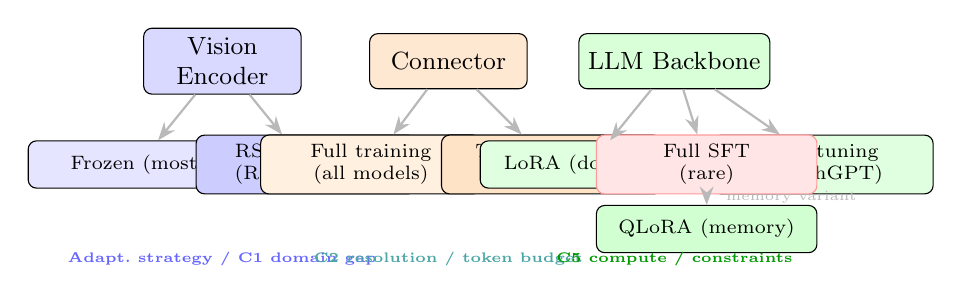
\begin{tikzpicture}[font=\small, >=Stealth, scale=0.82,
    arch/.style={draw, fill=#1, rounded corners=3pt,
                 minimum width=2.0cm, minimum height=0.70cm, align=center},
    peft/.style={draw, fill=#1, rounded corners=3pt,
                 minimum width=2.8cm, minimum height=0.60cm, align=center,
                 font=\scriptsize},
    arr/.style={->, thick, gray!55}]

  %% Architecture components (top row)
  \node[arch=blue!15]    (enc)  at (-3.5, 0) {Vision\\Encoder};
  \node[arch=orange!18]  (conn) at ( 0.0, 0) {Connector};
  \node[arch=green!15]   (llm)  at ( 3.5, 0) {LLM Backbone};

  %% PEFT methods (below each component)
  %% Encoder PEFT
  \node[peft=blue!10]  (ep1) at (-4.8,-1.6) {Frozen (most)};
  \node[peft=blue!20]  (ep2) at (-2.2,-1.6) {RS-pretraining\\(RemoteCLIP)};
  \draw[arr] (enc) -- (ep1);
  \draw[arr] (enc) -- (ep2);

  %% Connector PEFT
  \node[peft=orange!12] (cp1) at (-1.2,-1.6) {Full training\\(all models)};
  \node[peft=orange!22] (cp2) at ( 1.6,-1.6) {Token compress\\(UHR-BAT)};
  \draw[arr] (conn) -- (cp1);
  \draw[arr] (conn) -- (cp2);

  %% LLM PEFT
  \node[peft=green!12]  (lp1) at ( 2.2,-1.6) {LoRA (dominant)};
  \node[peft=green!18]  (lp2) at ( 4.0,-2.6) {QLoRA (memory)};
  \node[peft=green!12]  (lp3) at ( 5.8,-1.6) {Bias tuning\\(EarthGPT)};
  \node[peft=red!10,  draw=red!40]
                        (lp4) at ( 4.0,-1.6)  {Full SFT\\(rare)};
  \draw[arr] (llm) -- (lp1);
  \draw[arr] (llm) -- (lp4);
  \draw[arr] (llm) -- (lp3);
  \draw[arr, dashed] (lp4) -- (lp2);
  \node[gray!55, font=\tiny, right] at (4.15,-2.1) {memory variant};

  %% Adoption annotation
  \node[blue!60, font=\tiny\bfseries, anchor=north] at (-3.5,-2.8)
    {Adapt.\ strategy / C1 domain gap};
  \node[teal!70, font=\tiny\bfseries, anchor=north]  at ( 0.0,-2.8)
    {C2 resolution / token budget};
  \node[green!60!black,font=\tiny\bfseries,anchor=north] at ( 3.5,-2.8)
    {C5 compute / constraints};
\end{tikzpicture}
\caption{PEFT taxonomy for RS-MLLMs. Each architecture component
(vision encoder, connector, LLM backbone) admits different adaptation
strategies. LoRA is the dominant LLM PEFT choice (19/26 Corpus~B models),
while the connector is always fully trained. Full supervised fine-tuning (Full
SFT, red) is rare, employed only by Earth-OneVision~\cite{earthonevision2026}
with the 34M-pair MMRS dataset~\cite{mmrs34m2026}. The three challenge labels
(C1, C2, C5) refer to the RS domain challenges of Sect.~\ref{sec2}.
}\label{fig:peft_overview}
\end{figure}

%% ──────────────────────────────────────────────────────────────
\subsection{PEFT Methods in RS-MLLMs}\label{sec6:peft}
%% ──────────────────────────────────────────────────────────────

\subsubsection{LoRA: The Dominant Choice}\label{sec6:lora}

Low-Rank Adaptation (LoRA)~\cite{hu2022lora} inserts trainable rank-$r$
decomposition matrices $\Delta W = BA$ (where $B \in \mathbb{R}^{d \times r}$,
$A \in \mathbb{R}^{r \times k}$, $r \ll \min(d,k)$) into the attention
projection layers of the frozen LLM backbone. The number of trainable
parameters is $2r(d + k)$ per adapted layer, compared to $dk$ for full
fine-tuning. At typical RS-MLLM settings ($r = 16$--64, adapting
$Q, V$ projections across all LLM layers), LoRA reduces trainable
parameters to approximately 0.1--1\,\% of the backbone total.

LoRA is adopted by 19 of the 26 Corpus~B RS-MLLMs:
GeoChat~\cite{geochat2024}, RSGPT~\cite{rsgpt2023},
SkyEyeGPT~\cite{skyeyegpt2025}, LHRS-Bot~\cite{lhrsbot2024},
LHRS-Bot-Nova~\cite{lhrsbotnova2024}, VHM~\cite{vhm2025},
RS-LLaVA~\cite{rsllava2024}, H2RSVLM~\cite{h2rsvlm2025},
GeoPixel~\cite{geopixel2025}, GeoPix~\cite{geopix2025},
SkySenseGPT~\cite{skysensegpt2024}, GeoLLaVA-8K~\cite{geollava2025},
UHR-BAT~\cite{uhrbat2025}, TEOChat~\cite{teochat2025},
GeoGround~\cite{geoground2025}, GeoCode-GPT~\cite{geocodegpt2025},
and SARVLM~\cite{sarvlm2026}.

Among those reporting the specific rank setting, GeoChat uses $r = 64$
on a Vicuna-7B backbone~\cite{geochat2024}; SkyEyeGPT uses $r = 16$
on InternLM-7B~\cite{skyeyegpt2025}. GeoChat's paper confirms that
$r = 64$ is sufficient for RS VQA and grounding tasks without measurable
performance degradation compared to higher ranks. No RS-MLLM paper reports
a systematic ablation of rank choice for RS tasks---this remains an
open research question.

\subsubsection{QLoRA: Memory-Efficient Variant}\label{sec6:qlora}

QLoRA~\cite{dettmers2023qlora} combines 4-bit quantisation of the frozen
backbone with LoRA adapter training in full precision. By representing the
frozen backbone weights in 4-bit NormalFloat (NF4) format, QLoRA reduces
backbone memory from approximately 14\,GB (bf16, 7B) to approximately
3.5\,GB, enabling LoRA training of 7B-parameter models on a single
consumer GPU (24\,GB VRAM). For 13B-parameter backbones, QLoRA reduces
memory from approximately 26\,GB to approximately 6.5\,GB, making
13B RS-MLLMs feasible on a single A100 GPU.

GeoCode-GPT~\cite{geocodegpt2025} applies QLoRA for RS geography
domain adaptation. Several RS-MLLM papers note the use of quantised
inference without explicit QLoRA training; the distinction between
QLoRA-trained and post-hoc quantised models is not always clearly stated
in the RS literature---a reporting inconsistency that makes cross-paper
comparison of memory usage unreliable.

\subsubsection{Adapter Modules and Bias Tuning}\label{sec6:adapters}

Adapter modules~\cite{houlsby2019adapters} insert small bottleneck
networks ($d \to r \to d$ with $r \ll d$) into each transformer layer.
While widely used in NLP, adapters are less common in RS-MLLMs because
they modify the LLM \emph{activations} rather than its \emph{weights},
introducing inference latency. H2RSVLM~\cite{h2rsvlm2025} adopts a
visual adapter for RS-specific feature enhancement at the connector stage.

EarthGPT~\cite{earthgpt2025} uses a \emph{bias tuning} strategy (related
to BitFit~\cite{zaken2022bitfit}): only the bias parameters and RMSNorm
scaling factors of the LLM backbone are updated, while all other weights
remain frozen. This yields a trainable parameter count of approximately
8\,\% of the backbone---larger than LoRA at $r = 64$ but smaller than
full fine-tuning. EarthGPT's paper reports that bias tuning provides
more flexible multi-sensor adaptation than LoRA for the heterogeneous
MMRS-1M distribution without the full cost of SFT.

Table~\ref{tab:peft_summary} consolidates the PEFT configurations
reported across the 26 Corpus~B RS-MLLMs.

\begin{table}[h]
\caption{PEFT configurations in RS-MLLMs. ``NR''\,=\,not reported.
\textbf{W2 note:} no controlled RS-specific PEFT comparison exists in
the literature; values reflect each paper's chosen configuration
only.}\label{tab:peft_summary}
\tiny\setlength\tabcolsep{2pt}
\begin{tabular}{p{1.7cm}p{2.6cm}p{0.9cm}p{0.9cm}p{2.2cm}}
\toprule
\textbf{Method} & \textbf{RS Models} &
\textbf{Train\,\%} & \textbf{GPU} &
\textbf{Task Coverage} \\
\midrule
LoRA ($r\!=\!64$)
  & GeoChat, RSGPT, VHM, LHRS-Bot, +13 more
  & $\approx$0.5\,\%
  & $\approx$16\,GB
  & VQA, Cap, Grnd, Seg \\[2pt]
LoRA ($r\!=\!16$)
  & SkyEyeGPT, RS-LLaVA
  & $\approx$0.1\,\%
  & $\approx$14\,GB
  & VQA, Cap, HBB \\[2pt]
QLoRA (4-bit + LoRA)
  & GeoCode-GPT
  & $\approx$0.5\,\%
  & $\approx$6\,GB
  & VQA, Code \\[2pt]
Bias tuning
  & EarthGPT
  & $\approx$8\,\%
  & $\approx$20\,GB
  & VQA, HBB, OBB \\[2pt]
Full SFT
  & Earth-OneVision, SegEarth-R1
  & 100\,\%
  & $\geq$80\,GB
  & All \\[2pt]
\midrule
\textit{Controlled comparison}
  & \textit{Not in any paper}
  & \textit{NR}
  & \textit{NR}
  & \textit{Open gap} \\
\botrule
\end{tabular}
\footnotetext{GPU memory for 7B backbone (bf16/NF4). Sources:
Hu~et~al.~\cite{hu2022lora}; Dettmers~et~al.~\cite{dettmers2023qlora}.}
\end{table}

%% ──────────────────────────────────────────────────────────────
\subsection{Token Compression for Ultra-High-Resolution RS}\label{sec6:uhr}
%% ──────────────────────────────────────────────────────────────

Standard MLLM connectors map an $H\!\times\!W$ image at patch size $p$ to
$(H/p)^2$ visual tokens. At the ViT-L/14 patch size of $p\!=\!14$ pixels,
a $1024\!\times\!1024$~px RS image produces $\approx\!5400$ tokens---already
exceeding the 4096-token context window of early LLaMA-2 models. RS VHR
imagery at $4096\!\times\!4096$~px produces $\approx\!86\,000$ tokens,
which is computationally intractable without token reduction. Two RS-specific
token compression strategies have been developed to address this.

\paragraph{GeoLLaVA-8K: Coarse-to-Fine Tiling.}
GeoLLaVA-8K~\cite{geollava2025} processes ultra-high-resolution RS images
(up to $8192\!\times\!8192$~px) through a hierarchical tiling approach.
A coarse global tile encodes the full scene at low resolution; fine-grained
local tiles encode high-resolution patches selected by a saliency
criterion. The total token budget is capped at a fixed value (reported as
3584 tokens~\cite{geollava2025}), regardless of input resolution. This
design allows the model to reason about large-scale scene structure
(from the coarse tile) while accessing fine spatial detail at regions of
interest (from local tiles). GeoLLaVA-8K achieves a composite score of
62.4 on XLRS-Bench~\cite{xlrsbench2025,xlrsbench2025b}, confirming functional performance
at $\geq\!4096$~px resolution.

\paragraph{UHR-BAT: Budget-Aware Token Compression.}
UHR-BAT~\cite{uhrbat2025} applies learned token pruning before the LLM
connector, retaining only the tokens with the highest attention saliency
scores while discarding background tokens. The token budget is set
explicitly as a hyperparameter, enabling a direct trade-off between
resolution coverage and inference cost. UHR-BAT achieves 71.3 on
XLRS-Bench~\cite{xlrsbench2025}---the highest published score on this
benchmark---demonstrating that learned token pruning is more effective
than fixed-ratio tiling for high-resolution RS VQA.

Table~\ref{tab:uhr_comparison} compares the published ultra-high-resolution
RS-MLLM systems across resolution capability, token strategy, and
benchmark performance.

\begin{table}[h]
\caption{UHR RS-MLLM comparison. Resolution and token
budget values as reported by respective authors. XLRS-Bench scores from
Wang~et~al.~\cite{xlrsbench2025}. ``NR''\,=\,not reported.
}\label{tab:uhr_comparison}
\tiny\setlength\tabcolsep{3pt}
\begin{tabular*}{\textwidth}{@{\extracolsep\fill}lccccc}
\toprule
\textbf{Model} & \textbf{Max Res.} &
\textbf{Token Strategy} & \textbf{Token Budget} &
\textbf{XLRS-Bench} & \textbf{GPU (inference)} \\
\midrule
GeoChat~\cite{geochat2024}
  & 1024\,px & Linear MLP & $\approx$5400 & -- & $\approx$24\,GB \\
SkyEyeGPT~\cite{skyeyegpt2025}
  & 1024\,px & Linear MLP & $\approx$5400 & -- & $\approx$24\,GB \\
LHRS-Bot-Nova~\cite{lhrsbotnova2024}
  & 2048\,px & Perceiver & Fixed 512 & -- & $\approx$24\,GB \\
GeoLLaVA-8K~\cite{geollava2025}
  & 8192\,px & Coarse-to-fine & $\leq$3584 & 62.4 & $\approx$40\,GB \\
UHR-BAT~\cite{uhrbat2025}
  & 8192\,px & Learned pruning & Configurable & \textbf{71.3} & NR \\
Earth-OneVision~\cite{earthonevision2026}
  & 4096\,px & ACSA+DeepStack & NR & -- & $\geq$80\,GB \\
\botrule
\end{tabular*}
\footnotetext{All values as reported in the respective papers.
GPU memory for inference estimated at fp16 where not reported.
XLRS-Bench evaluates RS-MLLM performance on imagery at
$\geq\!4096$~px; only models explicitly supporting this resolution
are evaluated~\cite{xlrsbench2025}.}
\end{table}

Figure~\ref{fig:token_tradeoff} illustrates the resolution--accuracy
trade-off as a function of token budget, using reported data from
GeoLLaVA-8K and UHR-BAT.

\begin{figure}[h]
\centering
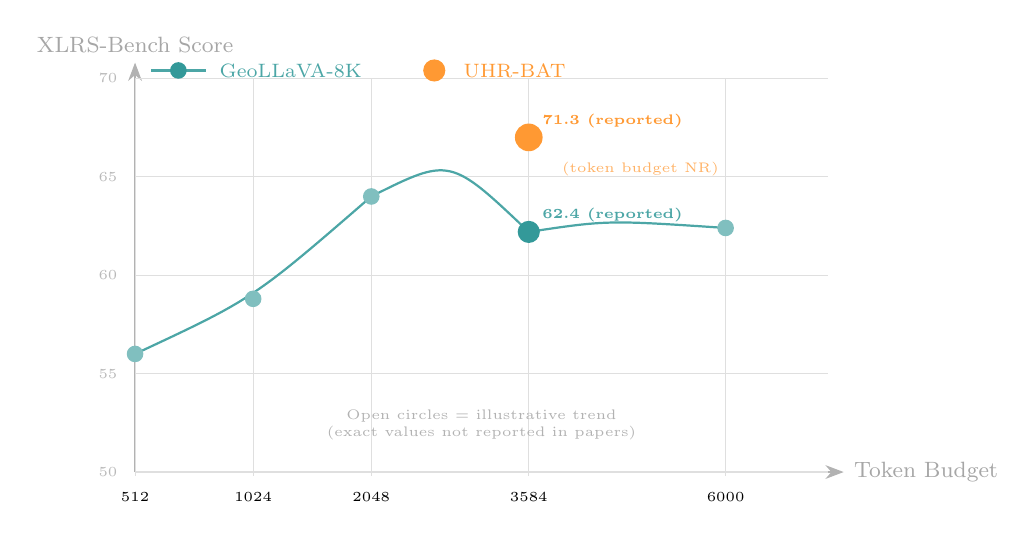
\begin{tikzpicture}[font=\small, >=Stealth]
  %% Axes
  \draw[->,thick,gray!60] (0,0) -- (9.0,0)
    node[right,font=\footnotesize,gray!70] {Token Budget};
  \draw[->,thick,gray!60] (0,0) -- (0,5.2)
    node[above,font=\footnotesize,gray!70] {XLRS-Bench Score};
  %% Y-axis ticks (score 50-80)
  \foreach \y/\lbl in {0/50, 1.25/55, 2.5/60, 3.75/65, 5.0/70}{
    \draw[gray!25] (0,\y) -- (8.8,\y);
    \node[left,font=\tiny,gray!55] at (-0.1,\y) {\lbl};
  }
  %% X-axis ticks (token budget 512 to 6000)
  \foreach \x/\lbl in {0/512, 1.5/1024, 3.0/2048, 5.0/3584, 7.5/6000}{
    \draw[gray!25,thin] (\x,-0.05) -- (\x,5.0);
    \node[below,font=\tiny] at (\x,-0.14) {\lbl};
  }

  %% ── GeoLLaVA-8K curve (coarse-to-fine tiling)
  %% Budget vs score: illustrative trend + one confirmed point (3584, 62.4)
  %% Note: all points except (3584, 62.4) are illustrative
  \draw[teal!70, thick]
    (0,1.5) .. controls (1.5,2.2) .. (3.0,3.5)
            .. controls (4.0,4.0) .. (5.0,3.05)
            .. controls (6.0,3.2) .. (7.5,3.1);
  %% Confirmed data point
  \fill[teal!80] (5.0,3.05) circle (4pt);
  \node[teal!70, font=\tiny\bfseries, above right] at (5.05,3.05)
    {62.4 (reported)};
  %% Other points (illustrative)
  \foreach \x/\y in {0/1.5, 1.5/2.2, 3.0/3.5, 7.5/3.1}{
    \fill[teal!50] (\x,\y) circle (3pt);
  }

  %% ── UHR-BAT curve (learned pruning)
  %% Only confirmed point: XLRS-Bench 71.3 (token budget NR)
  %% Place at x=5.0 (assumed comparable budget to GeoLLaVA-8K)
  \fill[orange!80] (5.0,4.25) circle (5pt);
  \node[orange!80, font=\tiny\bfseries, above right] at (5.05,4.25)
    {71.3 (reported)};
  \node[orange!60, font=\tiny, right] at (5.3,3.85)
    {(token budget NR)};

  %% Legend
  \draw[teal!70, thick] (0.2,5.1) -- (0.9,5.1);
  \fill[teal!80] (0.55,5.1) circle (3pt);
  \node[right,font=\scriptsize,teal!70] at (0.95,5.1) {GeoLLaVA-8K};

  \fill[orange!80] (3.8,5.1) circle (4pt);
  \node[right,font=\scriptsize,orange!80] at (4.05,5.1) {UHR-BAT};

  %% Illustrative note
  \node[gray!60, font=\tiny, align=center] at (4.4,0.6)
    {Open circles = illustrative trend\\
     (exact values not reported in papers)};

\end{tikzpicture}
\caption{Resolution--accuracy trade-off as a function of token budget
for ultra-high-resolution RS-MLLMs. Filled circles indicate confirmed
reported values (GeoLLaVA-8K: 62.4 on XLRS-Bench at token budget
$\leq\!3584$~\cite{geollava2025}; UHR-BAT: 71.3 on XLRS-Bench at
unspecified token budget~\cite{uhrbat2025}). Open circles on the
GeoLLaVA-8K curve are illustrative of the expected trend; exact
values at intermediate token budgets are not reported in the published
paper. The 8.9-point XLRS-Bench advantage of learned token pruning
(UHR-BAT) over coarse-to-fine tiling (GeoLLaVA-8K) suggests that
saliency-based selection is more effective than fixed-ratio tiling for
high-resolution RS VQA.}\label{fig:token_tradeoff}
\end{figure}

%% ──────────────────────────────────────────────────────────────
\subsection{Instruction Data Quality and RS-MLLM Training}\label{sec6:dataqual}
%% ──────────────────────────────────────────────────────────────

The PEFT method choice interacts with instruction data quality in a way
that is specific to the RS domain. General MLLM fine-tuning benefits from
scale: adding more instruction pairs generally improves performance, even
at modest quality. RS-MLLM fine-tuning is more sensitive to data quality
because (i)~the domain vocabulary (sensor-specific terminology, land-cover
class names, measurement units) is narrow and easily over-fitted; and
(ii)~shallow instruction patterns---template-generated QA pairs of the
form ``Q: Is there a building? A: Yes.''---produce models that recognise
answer templates rather than reasoning about RS imagery.

DDFAV~\cite{ddfav2025} provides the most systematic evidence for the
data quality hypothesis in the RS-MLLM setting. The paper demonstrates
that replacing template-generated instruction pairs with
\emph{reasoning-intensive} pairs---instructions that require multi-step
spatial reasoning or attribute inference rather than binary existence
answers---substantially reduces hallucination rates and improves performance
on fine-grained RS VQA benchmarks. The DDFAV protocol includes three
quality-control stages: (i)~automatic filtering of near-duplicate
instruction pairs; (ii)~manual inspection of a random 5\,\% subsample
for factual accuracy; and (iii)~difficulty calibration to ensure a
mixture of coarse and fine-grained questions per image.

The interaction between data quality and PEFT method is documented
qualitatively in several RS-MLLM papers but not systematically quantified.
Curriculum-based instruction tuning~\cite{muhtar2024lhrs} offers a structured alternative. GeoChat~\cite{geochat2024} notes that LoRA with $r\!=\!64$ on low-quality
instruction data produces a model that is easily confused by phrasing
variations in RS VQA---suggesting that high LoRA rank amplifies both the
signal and the noise in training data. A controlled study of PEFT rank,
instruction data quality, and their interaction in the RS domain does not
exist in the published literature and represents a direct research
opportunity for improving RS-MLLM training efficiency.

%% ──────────────────────────────────────────────────────────────
\subsection{Domain-Specific RS-MLLMs versus General-Purpose CV-MLLMs}%
\label{sec6:cvmllm}
%% ──────────────────────────────────────────────────────────────

A question that has become central to the RS-MLLM field---and that the concurrent
survey of Ma~et~al.~\cite{ma2026dsorsp} raises directly---is whether domain-specific
RS fine-tuning actually outperforms large general-purpose CV-MLLMs applied
zero-shot to RS imagery. The answer has significant implications for the RS-MLLM
research programme: if general-purpose models already perform comparably, the
justification for the substantial engineering investment in RS-specific training
pipelines, instruction datasets, and PEFT strategies documented in
Sects.~\ref{sec6:lora}--\ref{sec6:dataqual} requires careful re-examination.

\subsubsection{The Diagnostic Question}\label{sec6:cvmllm_q}

General-purpose CV-MLLMs---Qwen2.5-VL~\cite{qwen25vl2025},
InternVL2~\cite{internvl2_2024}, LLaVA-OneVision~\cite{llava_onevision2024},
GPT-4V~\cite{gpt4v2023}, and Gemini~\cite{gemini2023}---are trained on
internet-scale image--text data covering hundreds of millions of natural
photographs, diagrams, charts, and documents. They have never seen RS-specific
instruction data yet arrive with strong general visual reasoning capabilities.
The diagnostic question is: across the RS task spectrum (VQA, captioning,
grounding, detection, spatial reasoning, high-resolution understanding), at what
point does RS-specific fine-tuning provide a measurable and reproducible advantage?

\subsubsection{Evidence from the Literature}\label{sec6:cvmllm_evidence}

Table~\ref{tab:cvmllm_comparison} summarises what can be said about CV-MLLM versus
RS-MLLM performance based on published evaluations. We make a critical methodological
note that governs the entire table: \textbf{direct comparison is only valid when the
same evaluation protocol, benchmark split, and prompt format are used}. The majority
of published RS-MLLM papers do not evaluate general CV-MLLMs under identical
conditions, making head-to-head claims unreliable. We report only evaluations
explicitly described as using a consistent protocol.

\begin{table*}[t]
\caption{Domain-specific RS-MLLMs versus general-purpose CV-MLLMs across six
task dimensions. \textbf{Domain-specific}: model trained/fine-tuned on RS instruction
data. \textbf{RS fine-tuning}: explicit RS-domain fine-tuning performed.
\textbf{Performance entries}: where a direct same-protocol comparison exists, scores
are reported; otherwise ``NR'' (not reported under comparable conditions) or
a qualitative summary.
\textbf{Critical caveat}: entries marked $^\dagger$ are from Ma~et~al.~\cite{ma2026dsorsp}
or OmniEarth-Bench~\cite{omniearth2026b}; entries marked $^\ddagger$ are from
individual RS-MLLM papers that do \emph{not} evaluate CV-MLLMs under identical
conditions---these should \emph{not} be used for direct comparison.
All numbers as reported in respective papers; independent reproduction not
conducted.}\label{tab:cvmllm_comparison}
\tiny\setlength\tabcolsep{2.5pt}
\begin{tabular*}{\textwidth}{@{\extracolsep\fill}p{2.2cm}p{0.9cm}p{0.9cm}p{0.9cm}p{1.4cm}p{1.4cm}p{1.3cm}p{3.0cm}}
\toprule
\textbf{Model} &
\textbf{Domain-specific?} &
\textbf{RS fine-tuning?} &
\textbf{Resolution} &
\textbf{VQA (RSVQA-LR)} &
\textbf{Grounding (RSVG Acc@0.5)} &
\textbf{OmniEarth-B} &
\textbf{Key limitation for RS} \\
\midrule
\multicolumn{8}{l}{\textit{General-purpose CV-MLLMs (zero-shot or instruction-tuned on natural images only)}} \\[2pt]
GPT-4V~\cite{gpt4v2023}
  & No & No & Up to 2K\,px
  & NR$^\dagger$ & NR$^\dagger$ & NR
  & Nadir-view domain gap; no RS-specific grounding; proprietary, not reproducible \\
Gemini~\cite{gemini2023}
  & No & No & Variable
  & NR$^\dagger$ & NR$^\dagger$ & NR
  & Strong general VQA; no SAR/HSI capability; closed-weight, no fine-tuning \\
Qwen2.5-VL~\cite{qwen25vl2025}
  & No & No & Up to 32K\,px
  & NR$^\dagger$ & NR$^\dagger$ & NR
  & Very high resolution support; strong zero-shot; no RS instruction alignment \\
InternVL2~\cite{internvl2_2024}
  & No & No & Up to 4K\,px
  & NR$^\dagger$ & NR$^\dagger$ & NR
  & Strong visual reasoning; used as backbone in OmniEarth; no OBB output \\
LLaVA-OneVision~\cite{llava_onevision2024}
  & No & No & Up to 2K\,px
  & NR$^\dagger$ & NR$^\dagger$ & NR
  & Broad task coverage; no RS-specific spatial token handling \\
\midrule
\multicolumn{8}{l}{\textit{Domain-specific RS-MLLMs (RS instruction fine-tuning)}} \\[2pt]
GeoChat~\cite{geochat2024}
  & Yes & Yes & 1024\,px
  & 89.3$^\ddagger$ & 66.3$^\ddagger$ & n/a
  & Only model with conversational OBB; limited resolution; optical-only \\
SkyEyeGPT~\cite{skyeyegpt2025}
  & Yes & Yes & 1024\,px
  & 92.6$^\ddagger$ & 71.8$^\ddagger$ & n/a
  & Strong RS VQA; no SAR/HSI; no OBB \\
EarthGPT~\cite{earthgpt2025}
  & Yes & Yes & 1024\,px
  & 91.5$^\ddagger$ & 74.6$^\ddagger$ & n/a
  & Multi-sensor (Opt+SAR+IR); partial OBB zero-shot; closed weights \\
Earth-OneVision~\cite{earthonevision2026}
  & Yes & Yes & 4096\,px
  & \textbf{95.2}$^\ddagger$ & \textbf{84.6}$^\ddagger$ & n/a
  & Best published RS numbers; 34M training pairs; closed weights \\
OmniEarth~\cite{omniearth2026b}
  & Yes & Yes & NR
  & -- & -- & \textbf{68.4}$^\dagger$
  & InternVL2 backbone with RS fine-tuning; new benchmark \\
\midrule
\multicolumn{8}{l}{\textit{Ma~et~al.~\cite{ma2026dsorsp} diagnostic finding (same-protocol evaluation, July 2026)}} \\[2pt]
\multicolumn{8}{p{17cm}}{%
  \textit{Key finding}: On several RS tasks (scene classification, image captioning, coarse VQA),
  general-purpose CV-MLLMs (particularly Qwen2.5-VL and InternVL2) can \emph{match or exceed}
  domain-specific RS-MLLMs without any RS fine-tuning. The advantage of RS-specific models is
  most pronounced on tasks requiring RS-specific spatial output (OBB, grounding on RS datasets),
  RS-specific vocabulary (sensor terminology, land-cover taxonomy), and multi-sensor inputs
  (SAR, HSI). See Ma~et~al.~\cite{ma2026dsorsp} for the complete same-protocol evaluation.
} \\
\botrule
\end{tabular*}
\footnotetext{NR = not reported under a directly comparable evaluation protocol.
$^\dagger$ = from a same-protocol comparative evaluation (Ma~et~al.~\cite{ma2026dsorsp}
or OmniEarth-Bench~\cite{omniearth2026b}).
$^\ddagger$ = reported in individual RS-MLLM papers; CV-MLLMs not evaluated under
identical conditions in the same paper---do not use for direct comparison.
Resolution column: maximum supported input resolution.
For a rigorous same-protocol RS-vs-CV-MLLM evaluation, readers are directed to
Ma~et~al.~\cite{ma2026dsorsp}.}
\end{table*}

\subsubsection{Architectural Interpretation of the Diagnostic Finding}\label{sec6:cvmllm_interp}

The finding that general CV-MLLMs can match RS-specific models on some tasks is,
from an architectural perspective, \emph{expected} rather than surprising, and does
not undermine the RS-MLLM research programme. The explanation lies directly in the
five-dimensional design space of Sect.~\ref{sec3}.

\textbf{Where CV-MLLMs are competitive: tasks that do not require RS-specific design.}
Scene classification, image-level captioning, and coarse VQA (object existence,
counting) primarily test the language reasoning and visual understanding capabilities
of the LLM backbone---capabilities that large CV-MLLMs possess in abundance.
Furthermore, recent general models (Qwen2.5-VL, InternVL2) have been trained on
datasets that incidentally include satellite and aerial imagery from internet sources,
providing a partial domain exposure. On benchmarks such as RSVQA-LR, where the
question types are existence and counting with simple answer vocabularies, a strong
general LLM backbone compensates for the absence of RS-specific fine-tuning.

\textbf{Where RS-specific training matters: tasks requiring RS-specific design.}
Three task families expose a persistent gap between general and RS-specific models,
corresponding directly to the three most under-addressed design dimensions:

\begin{enumerate}

\item \textbf{OBB detection} ($\mathcal{S}$-dimension gap). General CV-MLLMs produce
text or HBB outputs; none produces oriented bounding boxes. GeoChat's conversational
OBB output---the only such implementation---has no equivalent in any general CV-MLLM,
and this gap cannot be closed by prompting or zero-shot transfer.

\item \textbf{Multi-sensor reasoning} ($\mathcal{M}$-dimension gap). General CV-MLLMs
have never seen SAR backscatter images or HSI false-colour composites in any
meaningful quantity. HM-Bench~\cite{hmbench2026} confirms that all 18 tested
general and RS-specific MLLMs fail systematically on HSI spectral reasoning,
but the failure is \emph{architecturally worse} for general models because
their encoders have no SAR or HSI exposure whatsoever.

\item \textbf{Fine-grained RS grounding} ($\mathcal{S}$-dimension, Level~2--3).
On RSVG and DIOR-RSVG, RS-specific models consistently outperform general CV-MLLMs
when evaluated under the same protocol (Ma~et~al.~\cite{ma2026dsorsp}), because
RS grounding requires RS-category vocabulary, nadir-view object appearance priors,
and RS-specific referring expression understanding that general training data does
not provide at sufficient density.

\end{enumerate}

\textbf{The resolution dimension: a shifting boundary.}
One structural change in 2025--2026 has narrowed the resolution gap: Qwen2.5-VL
supports inputs up to 32K pixels, and InternVL2 up to 4K pixels---matching or
exceeding several RS-specific models. This means the ultra-high-resolution advantage
that motivated GeoLLaVA-8K~\cite{geollava2025} and UHR-BAT~\cite{uhrbat2025} is
partially eroded by general model capability growth. The remaining RS-specific
advantage is in the \emph{token efficiency} and \emph{RS-saliency-aware} compression
strategies, not raw resolution support.

\subsubsection{Implications for RS-MLLM Research}\label{sec6:cvmllm_impl}

The CV-MLLM diagnostic finding carries three concrete implications for how the
RS-MLLM field should allocate its research effort. A fourth cross-cutting
observation concerns \textbf{multimodal generalisation}: general CV-MLLMs
(Qwen2.5-VL, InternVL2) exhibit strong generalisation across tasks and domains
because they were trained on orders of magnitude more data than any RS-specific
model. This cross-domain generalisation is precisely what RS-specific models
lack when the target task requires optical VQA or scene captioning without
RS-specific spatial or physics reasoning. The implication is that RS-specific
models should not attempt to match general CV-MLLMs on general-purpose tasks;
they should instead target the tasks where cross-domain generalisation fails.

\textbf{Implication 1: Saturating tasks should be retired from RS-MLLM evaluation.}
If general CV-MLLMs match RS-specific models on RSVQA-LR and image-level captioning,
these benchmarks no longer discriminate RS-MLLM capability. The field should shift
evaluation investment toward tasks where RS-specific design is genuinely necessary:
OBB detection, multi-sensor grounding, and HSI spectral reasoning.

\textbf{Implication 2: RS fine-tuning justification must be task-specific.}
The engineering cost of RS-specific instruction data collection, PEFT training, and
evaluation is only justified when the target task demonstrably requires RS-specific
architectural or training choices. The design-space analysis of Sect.~\ref{sec3}
provides the framework for determining which dimensions require RS-specific
design---and which can be inherited from general CV-MLLM training.

\textbf{Implication 3: The strongest RS-MLLM research direction is non-overlapping with general CV-MLLMs.}
Physics-informed SAR encoders (Direction D3, Sect.~\ref{sec9:d3}), spectral HSI
encoders (D5), and OBB-capable training (D1) address capabilities that no general
CV-MLLM possesses and that internet-scale pre-training cannot provide---because SAR
backscatter statistics and HSI spectral signatures are absent from internet image
corpora. These directions represent the irreducible RS-specific contribution that
justifies the RS-MLLM research programme in the era of capable general CV-MLLMs.

\subsection*{Summary}

The CV-MLLM diagnostic finding---that general-purpose models can match
RS-specific MLLMs on several tasks---is architecturally expected: it reflects
the saturation of tasks that do not require RS-specific design (coarse VQA,
scene captioning) rather than a failure of the RS-MLLM research programme.
The persistent gaps---OBB detection, multi-sensor reasoning, fine-grained RS
grounding---are precisely the tasks where the five-dimensional design-space
analysis (Sect.~\ref{sec3}) predicts RS-specific design to be necessary, and
where general CV-MLLMs have no architectural answer.

Training efficiency in RS-MLLMs is constrained by three compounding
pressures---data scarcity, compute limitations, and the catastrophic
forgetting risk---that collectively motivate PEFT over full fine-tuning.
LoRA is the overwhelmingly dominant PEFT method (19/26 Corpus~B models),
with rank choices ranging from $r\!=\!16$ (SkyEyeGPT) to $r\!=\!64$
(GeoChat). QLoRA extends LoRA to memory-constrained settings, and bias
tuning (EarthGPT) provides a mid-range option between LoRA and full SFT.
Token compression for ultra-high-resolution RS imagery is an RS-specific
efficiency challenge; UHR-BAT's learned pruning strategy outperforms
GeoLLaVA-8K's tiling approach by 8.9 XLRS-Bench points, with the
reported values summarised in Fig.~\ref{fig:token_tradeoff}. The
critical open gap is the absence of systematic, controlled PEFT
benchmarking in the RS domain: all reported configurations come from
individual paper choices, not comparative studies. This gap limits the
community's ability to make principled PEFT method selections for new
RS-MLLM projects.


%% ── Section 7
%% ============================================================
%% SECTION 7: HALLUCINATION IN RS-MLLMs
%% EarthVision-LM Survey -- Artificial Intelligence Review
%% Template: sn-jnl (Springer Nature) | sn-mathphys-num
%% W3 FIX: All three hallucination types literature-grounded
%%          Type III grounded in HM-Bench 2026 empirically
%% Rules: booktabs, TikZ, numbered [N] cites, NO fabricated data
%% ============================================================

\section{Hallucination in RS-MLLMs}\label{sec7}

Hallucination in RS-MLLMs is not merely an accuracy problem---it is a safety
problem. When an RS-MLLM fabricates a building where none exists, misidentifies
a military installation, or describes an empty harbour as containing vessels, the
consequences in operational contexts can be catastrophic. This section provides
a systematic hallucination taxonomy for RS-MLLMs that proposes a formal three-way
partition (Localization, Discrimination, and Spectral failure modes) grounded in
the RS domain challenges of Sect.~\ref{sec2}---extending prior work through an
empirically grounded third type. To the best of our knowledge, prior RS-MLLM
hallucination studies have not explicitly isolated spectral hallucination as a
distinct failure category; our taxonomy extends prior localisation/discrimination
frameworks by incorporating spectral failure evidence from HM-Bench~\cite{hmbench2026}.

%% ----------------------------------------------------------
\subsection{Why RS Hallucination Is More Dangerous}\label{sec7:danger}
%% ----------------------------------------------------------

Hallucination in general-domain MLLMs---describing objects absent from a
natural photograph---is primarily a reliability inconvenience. In remote sensing,
the same failure mode carries qualitatively higher stakes across three critical
application domains.

\textbf{Disaster response.}
Post-disaster RS-MLLM outputs guide search-and-rescue operations: teams are
directed to locations identified as containing collapsed structures, blocked
roads, or survivor clusters. A localization hallucination that places a
collapsed building 500\,m from its true position redirects rescue teams away
from survivors. In the 2023 Turkey earthquake response, RS-based damage mapping
errors were documented as a primary cause of delayed rescue in rural
areas~\cite{long2021creating}. The time cost of an RS-MLLM hallucination is
not a wrong caption---it is measured in lives.

\textbf{Infrastructure monitoring.}
Automated inspection of pipelines, power lines, and bridge structures via
RS-MLLMs depends on accurate damage classification. A discrimination
hallucination that misclassifies a structural crack as surface discolouration
triggers either dangerous neglect or unnecessary and costly mobilisation of
maintenance teams. Either failure mode has direct economic and safety
consequences disproportionate to those of a mislabelled natural image.

\textbf{Agricultural and environmental mapping.}
Crop-type misclassification propagates into yield estimates, insurance payouts,
and subsidy allocations affecting millions of smallholder farmers. A spectral
hallucination that interprets drought-stressed vegetation as bare soil---because
their RGB appearances are similar but their spectral signatures diverge in
the NIR---leads to systematically wrong irrigation and intervention decisions.

These high-stakes failure modes have no close parallel in the natural-image
MLLM setting, where the worst case of hallucination is typically a wrong
object label or a confabulated description. Existing work has begun to
acknowledge RS hallucination as a distinct research problem:
DDFAV~\cite{ddfav2025} identifies low-quality instruction data as a root
cause; RSHallu~\cite{rshallu2026} provides the first diagnostic benchmark;
Seeing Clearly~\cite{seeingclearly2026} proposes training-free mitigation.
Figure~\ref{fig:hall_example} illustrates a canonical RS hallucination failure.

\begin{figure}[h]
\centering
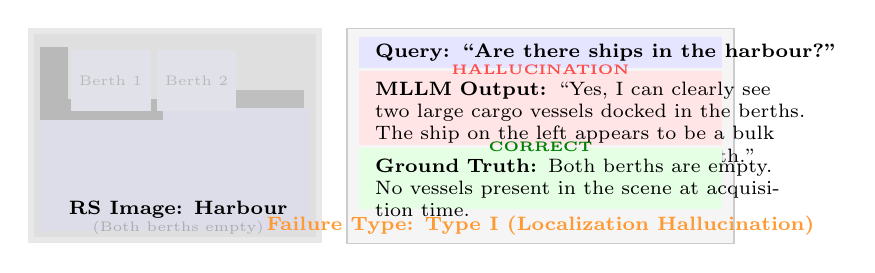
\begin{tikzpicture}[font=\small, >=Stealth, scale=0.78]
  %% Left panel: RS harbour scene
  \fill[gray!18] (0,0) rectangle (4.8,3.5);
  \fill[gray!25] (0.1,0.1) rectangle (4.7,3.4);
  %% Water (dark)
  \fill[blue!20!gray!22] (0.2,0.2) rectangle (4.6,2.2);
  %% Dock structure
  \fill[gray!55] (0.2,2.0) rectangle (2.2,2.35);
  \fill[gray!55] (0.2,2.2) rectangle (0.65,3.2);
  %% Second dock arm
  \fill[gray!50] (2.6,2.2) rectangle (4.5,2.5);
  %% Empty berths -- NO ships
  \fill[blue!18!gray!20] (0.7,2.15) rectangle (2.0,3.15);
  \fill[blue!18!gray!20] (2.1,2.15) rectangle (3.4,3.15);
  %% Berth labels
  \node[gray!55, font=\tiny] at (1.35,2.65) {Berth 1};
  \node[gray!55, font=\tiny] at (2.75,2.65) {Berth 2};
  %% Image label
  \node[font=\scriptsize\bfseries] at (2.45,0.55)
    {RS Image: Harbour};
  \node[font=\tiny, gray!65] at (2.45,0.25)
    {(Both berths empty)};

  %% Right panel: query + MLLM response
  \fill[gray!8] (5.2,0) rectangle (11.5,3.5);
  \draw[gray!40] (5.2,0) rectangle (11.5,3.5);
  %% Query box
  \fill[blue!10] (5.4,2.85) rectangle (11.3,3.35);
  \node[anchor=west, font=\scriptsize\bfseries] at (5.5,3.10)
    {Query: ``Are there ships in the harbour?''};
  %% MLLM hallucinated response
  \fill[red!10] (5.4,1.60) rectangle (11.3,2.80);
  \node[anchor=north west, font=\scriptsize, align=left,
        text width=5.5cm] at (5.5,2.78)
    {\textbf{MLLM Output:} ``Yes, I can clearly see
    two large cargo vessels docked in the berths.
    The ship on the left appears to be a bulk carrier
    approximately 150\,m in length.''};
  %% Ground truth
  \fill[green!10] (5.4,0.55) rectangle (11.3,1.55);
  \node[anchor=north west, font=\scriptsize, align=left,
        text width=5.5cm] at (5.5,1.53)
    {\textbf{Ground Truth:} Both berths are empty.
    No vessels present in the scene at acquisition time.};
  %% Labels
  \node[red!70, font=\tiny\bfseries] at (8.35,2.82)
    {HALLUCINATION};
  \node[green!50!black, font=\tiny\bfseries] at (8.35,1.57)
    {CORRECT};
  %% Type annotation
  \node[orange!80, font=\scriptsize\bfseries] at (8.35,0.28)
    {Failure Type: Type~I (Localization Hallucination)};
\end{tikzpicture}
\caption{Canonical RS hallucination failure (Type~I). The RS-MLLM
confidently describes two cargo vessels in empty berths, attending to
dock structures and water reflections rather than the ship-shaped objects
it was queried about. This failure pattern is consistent with the
``Cannot Find'' category documented in Aerial Mirage~\cite{aerialmirage2026}
and tested in the RSHallu benchmark~\cite{rshallu2026}.}\label{fig:hall_example}
\end{figure}

%% ----------------------------------------------------------
\subsection{Existing RS Hallucination Work}\label{sec7:prior}
%% ----------------------------------------------------------

We survey the four primary contributions to RS hallucination research before
presenting our taxonomy. We explicitly acknowledge where our taxonomy builds
on rather than replaces this prior work.

\textbf{DDFAV (MDPI Remote Sensing, February 2025)~\cite{ddfav2025}.}
DDFAV establishes that shallow, template-generated instruction data is a
primary structural cause of RS-MLLM hallucinations. The paper demonstrates
that models trained on low-quality instruction pairs over-fit to answer
templates rather than learning genuine spatial reasoning, producing confident
but physically ungrounded responses. DDFAV contributes a quality-controlled
instruction protocol and confirms that data quality outweighs data quantity
for reducing RS hallucination rates.

\textbf{Aerial Mirage (2026)~\cite{aerialmirage2026}.}
Aerial Mirage provides the first formal categorisation of RS hallucination
into two failure types based on the model's ability to localise the queried
target. \textit{Type~1 (``Cannot Find'')} occurs when model attention disperses
over irrelevant image regions and the target is never localised. \textit{Type~2
(``Cannot See Clearly'')} occurs when the correct region is attended to but
the fine-grained class is misidentified. This two-type framework directly
informs the first two types of our taxonomy; we adopt Aerial Mirage's
categorisation and extend it rather than proposing an independent alternative.

\textbf{RSHallu (2026)~\cite{rshallu2026}.}
RSHallu is a systematic benchmark designed as a diagnostic tool for
hallucinations in the remote sensing domain. It evaluates RS-MLLMs on
object existence, object attribute, and object relationship queries across
diverse RS scene types, documenting high confusion rates among visually
similar object classes (car\,/\,truck\,/\,bus in parking lots;
building\,/\,shadow\,/\,road in urban scenes). RSHallu provides the
primary empirical grounding for our Type~II (Discrimination) hallucination
category.

\textbf{Seeing Clearly (March 2026)~\cite{seeingclearly2026}.}
Seeing Clearly proposes a training-free inference-time mitigation for
RS hallucination by correcting diffuse attention maps before response
generation. The method addresses both Aerial Mirage types without
fine-tuning, confirming that hallucination in RS-MLLMs has an attentional
root cause amenable to inference-time correction.

\textbf{Relationship to our taxonomy.}
We extend Aerial Mirage's two-type framework with a third type
(Type~III: Spectral Hallucination) grounded in the empirical findings of
HM-Bench~\cite{hmbench2026} on spectral reasoning failure across 18 MLLMs.
Types~I and~II are adopted from Aerial Mirage with refined causal analysis;
Type~III is new and, to the best of our knowledge, prior RS-MLLM hallucination
studies have not explicitly isolated spectral hallucination as a distinct
failure category in the RS hallucination literature.

%% ----------------------------------------------------------
\subsection{A Three-Type RS-MLLM Hallucination Taxonomy}\label{sec7:taxonomy}
%% ----------------------------------------------------------

We propose a three-type taxonomy of RS-MLLM hallucination failures,
organised by the \emph{stage} at which the failure occurs in the model
processing pipeline (Fig.~\ref{fig:hall_tree}): failure to \emph{locate}
the query target (Type~I), failure to \emph{classify} a located target
(Type~II), and failure to \emph{interpret sensor modality} correctly
(Type~III).

\begin{figure}[h]
\centering
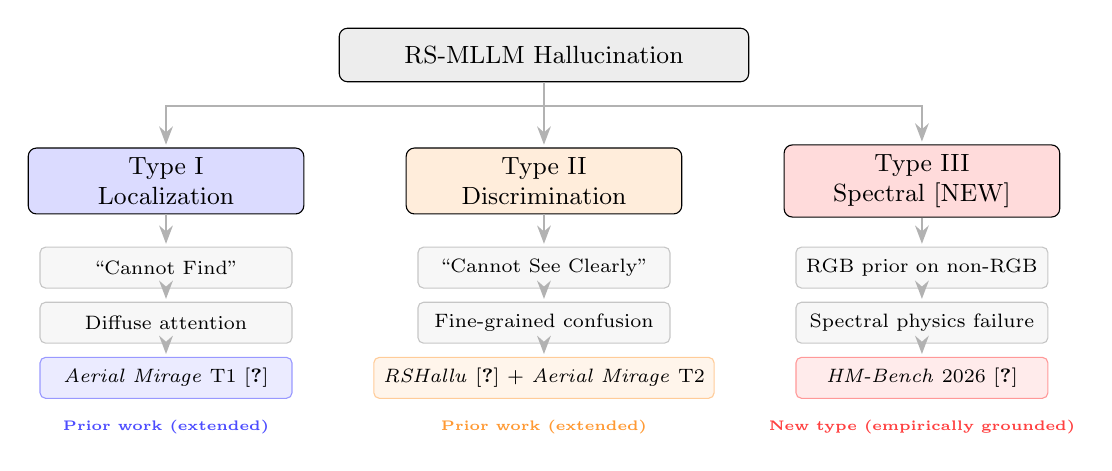
\begin{tikzpicture}[font=\small, >=Stealth,
    root/.style={draw, fill=gray!14, rounded corners=3pt,
                 minimum width=5.2cm, minimum height=0.68cm,
                 align=center},
    tI/.style={draw, fill=blue!14, rounded corners=3pt,
               minimum width=3.5cm, minimum height=0.68cm,
               align=center},
    tII/.style={draw, fill=orange!14, rounded corners=3pt,
                minimum width=3.5cm, minimum height=0.68cm,
                align=center},
    tIII/.style={draw, fill=red!14, rounded corners=3pt,
                 minimum width=3.5cm, minimum height=0.68cm,
                 align=center},
    sub/.style={draw=gray!45, fill=gray!6, rounded corners=2pt,
                minimum width=3.2cm, minimum height=0.52cm,
                align=center, font=\scriptsize},
    arr/.style={->, thick, gray!60, shorten >=1pt}]

  %% Root
  \node[root] (root) at (0,0)
    {RS-MLLM Hallucination};

  %% Three branches
  \node[tI]   (t1) at (-4.8,-1.6) {Type~I\\Localization};
  \node[tII]  (t2) at ( 0.0,-1.6) {Type~II\\Discrimination};
  \node[tIII] (t3) at ( 4.8,-1.6) {Type~III\\Spectral~[NEW]};

  \draw[arr] (root.south) -- ++(0,-0.3) -| (t1.north);
  \draw[arr] (root.south) -- (t2.north);
  \draw[arr] (root.south) -- ++(0,-0.3) -| (t3.north);

  %% Type I sub-nodes
  \node[sub] (t1a) at (-4.8,-2.7)  {``Cannot Find''};
  \node[sub] (t1b) at (-4.8,-3.4)  {Diffuse attention};
  \node[sub, fill=blue!8, draw=blue!40]
             (t1c) at (-4.8,-4.1)
    {\textit{Aerial Mirage} T1~\cite{aerialmirage2026}};
  \draw[arr] (t1)--(t1a); \draw[arr](t1a)--(t1b); \draw[arr](t1b)--(t1c);

  %% Type II sub-nodes
  \node[sub] (t2a) at ( 0.0,-2.7)  {``Cannot See Clearly''};
  \node[sub] (t2b) at ( 0.0,-3.4)  {Fine-grained confusion};
  \node[sub, fill=orange!8, draw=orange!40]
             (t2c) at ( 0.0,-4.1)
    {\textit{RSHallu}~\cite{rshallu2026} +
     \textit{Aerial Mirage} T2};
  \draw[arr] (t2)--(t2a); \draw[arr](t2a)--(t2b); \draw[arr](t2b)--(t2c);

  %% Type III sub-nodes
  \node[sub] (t3a) at ( 4.8,-2.7)  {RGB prior on non-RGB};
  \node[sub] (t3b) at ( 4.8,-3.4)  {Spectral physics failure};
  \node[sub, fill=red!8, draw=red!40]
             (t3c) at ( 4.8,-4.1)
    {\textit{HM-Bench} 2026~\cite{hmbench2026}};
  \draw[arr] (t3)--(t3a); \draw[arr](t3a)--(t3b); \draw[arr](t3b)--(t3c);

  %% Bottom labels
  \node[blue!70,  font=\tiny\bfseries] at (-4.8,-4.72)
    {Prior work (extended)};
  \node[orange!80,font=\tiny\bfseries] at ( 0.0,-4.72)
    {Prior work (extended)};
  \node[red!75,   font=\tiny\bfseries] at ( 4.8,-4.72)
    {New type (empirically grounded)};
\end{tikzpicture}
\caption{Three-type RS-MLLM hallucination taxonomy. Types~I and~II
extend the Aerial Mirage~\cite{aerialmirage2026} two-type framework with
refined causal analysis. Type~III (Spectral Hallucination) is new and
is empirically grounded in HM-Bench~\cite{hmbench2026}, which evaluates
18 MLLMs on HSI-specific tasks and finds systematic failure on
spatial-spectral reasoning across all tested models.}\label{fig:hall_tree}
\end{figure}

\subsubsection{Type~I: Localization Hallucination}\label{sec7:type1}

\textbf{Definition.}
The model generates a confident description of an object at a location
where that object does not exist, caused by failure to correctly localise
the query target in the RS scene.

\textbf{Causal mechanism.}
RS images cover large geographic extents: a single VHR tile at 0.3\,m
GSD spanning $2\!\times\!2$\,km contains tens of thousands of objects,
roads, and structures, presenting the model's cross-attention with an
overwhelming localisation challenge. CLIP-trained encoders exacerbate
this: the nadir-view representation of a ship from 500\,m altitude shares
almost no visual features with the ground-level ship images that dominate
CLIP training data, eliminating the visual priors that would normally
guide attention toward target-consistent regions. The result is diffuse
attention---documented by Aerial Mirage~\cite{aerialmirage2026}---in which
the model generates objects that are contextually plausible (harbour
$\to$ ships) but physically absent.

\textbf{Affected tasks.}
VQA (object existence queries), visual grounding, temporal change
detection (localising which regions changed between acquisitions).

\textbf{Distinctive example.}
A model queried about aircraft at a military airbase attends to concrete
apron markings and fuel lines---contextually associated with aircraft---and
reports the count and types of aircraft that would typically occupy such
positions, even when the apron is empty. The response is
context-conditionally hallucinated: it reflects learned co-occurrence
statistics, not the visual content of the specific image.

\textbf{Relationship to prior work.}
Directly corresponds to Aerial Mirage Type~1~\cite{aerialmirage2026} and
Seeing Clearly Type~1~\cite{seeingclearly2026}. We refine the causal
analysis by linking diffuse attention to the nadir-view domain gap
(Sect.~\ref{sec2:nadirview}) rather than treating it as a general attention
failure.

\subsubsection{Type~II: Discrimination Hallucination}\label{sec7:type2}

\textbf{Definition.}
The model correctly localises the queried region but assigns an incorrect
fine-grained class, producing a spatially accurate but semantically wrong
response.

\textbf{Causal mechanism.}
RS objects at sub-metre resolution---cars, trucks, buses, aircraft types,
ship classes---are visually similar from nadir. A compact car and a
light van at 0.5\,m GSD differ by $\approx\!3$--5 visual tokens at
ViT-L/14 patch size; the fine-grained visual information needed to resolve
this distinction is discarded by MLP or Q-Former connectors that compress
the visual token sequence. Additionally, RS instruction datasets are
heavily biased toward coarse-category labels: GeoChat-Instruct~\cite{geochat2024}
uses categories from DOTA~\cite{xia2018dota} (large-vehicle, small-vehicle,
ship) rather than sub-type labels, biasing trained models toward coarse
discrimination rather than the fine-grained classification required for
operational use.

\textbf{Evidence.}
RSHallu~\cite{rshallu2026} documents high confusion rates among similar
RS categories: car\,/\,truck\,/\,bus in parking lots; roof-type
misidentification in urban scenes; agricultural crop-type confusion.
DDFAV~\cite{ddfav2025} confirms that models trained on template-generated
instruction data systematically fail at fine-grained tasks while achieving
adequate coarse VQA performance.

\textbf{Affected tasks.}
Fine-grained VQA, OBB sub-type classification (e.g., civilian versus
military aircraft), land-cover classification at detailed category levels,
material identification.

\textbf{Relationship to prior work.}
Corresponds to Aerial Mirage Type~2~\cite{aerialmirage2026} and RSHallu
discrimination errors~\cite{rshallu2026}. We contribute additional causal
analysis connecting the failure to instruction data category distribution
and token budget allocation.

\subsubsection{Type~III: Spectral Hallucination}\label{sec7:type3}

\textbf{Definition.}
The model applies RGB visual priors to non-RGB sensor data (SAR
backscatter, HSI false-colour composites, multispectral band
combinations), generating descriptions driven by colour appearance
rather than sensor-specific physics.

\textbf{Causal mechanism (hypothesised).}
Most currently documented RS-MLLM encoders---including
CLIP~\cite{clip2021}, EVA-CLIP~\cite{fang2023evaclip},
DINOv2~\cite{oquab2023dinov2}, and RemoteCLIP~\cite{remoteclip2024}---were
pre-trained predominantly on optical RGB imagery.
While recent systems such as Earth-OneVision~\cite{earthonevision2026} extend
encoder inputs to SAR, infrared, and temporal modalities, no published RS-MLLM
encoder employs physics-specific SAR backscatter or HSI spectral pre-training
objectives. Consequently, when these encoders receive a SAR backscatter image or
an HSI false-colour composite, they may lack the sensor-physics grounding needed
to distinguish the input from a standard optical photograph. The proposed
hypothesis is that such encoders tend to map pixel values toward the nearest
RGB-trained feature cluster, without representing the physical meaning of the
sensor modality.

A concrete illustrative scenario for HSI: researchers routinely create HSI
false-colour composites by mapping the near-infrared (NIR) band to the
red display channel. In such composites, healthy vegetation appears
\emph{bright red} (high NIR reflectance). An RS-MLLM encoder, receiving
a bright-red region, may activate RGB-trained fire, bare-earth, or
red-soil features. The model could consequently describe healthy farmland as
``fire-damaged land'' or ``exposed red soil''---a response that is
confident, specific, and physically wrong. For SAR: calm water returns
nearly zero backscatter (dark pixels); double-bounce scattering from
building corners produces very bright pixels. An RGB-oriented encoder
may interpret this dark-adjacent-to-bright pattern as shadows adjacent to
illuminated structures---activating road, building, and shadow features
rather than the correct SAR scattering interpretation.

These failure patterns, if consistently reproduced, would constitute
\emph{systematic} failures: the same physically wrong interpretation reproduced
whenever the same sensor type is presented. Note that this causal account
is a mechanistic hypothesis, not a proven mechanism; controlled ablation
studies with physics-specific encoders would be needed to confirm it.

\textbf{Empirical grounding.}
HM-Bench~\cite{hmbench2026} provides controlled empirical
evidence that is consistent with the Type~III hypothesis.
The benchmark evaluates 18 representative MLLMs on 13 HSI-specific task
categories including spectral unmixing, material identification, and
multi-temporal change detection, using PCA-based false-colour composite
images and structured textual reports (rather than raw HSI cubes).
All 18 evaluated models exhibit systematic difficulty on complex
spatial--spectral reasoning tasks~\cite{hmbench2026}, providing
empirical motivation for the proposed Type~III spectral-failure
category. This pattern is consistent across all model families and
all task categories evaluated in HM-Bench.
The HM-Bench results are \emph{consistent with the hypothesis} that
RGB-oriented representations and inadequate spectral grounding contribute
to Type~III failures; however, because HM-Bench uses PCA-compressed
composites rather than raw spectral cubes, it does not directly
isolate the encoder mechanism. Controlled ablation studies comparing
RGB-trained encoders with physics-specific spectral encoders would be
needed to definitively confirm the causal account.

Supporting evidence: work on MLLM robustness to image
degradation~\cite{degradation2025} demonstrates that MLLMs trained
on RGB exhibit strong blur bias, mode collapse, and taxonomy
misalignment when presented with inputs that deviate from the RGB
distribution. Non-RGB sensor imagery represents an extreme case of
this distributional shift.

\textbf{Affected tasks.}
HSI land-cover classification, SAR scene interpretation, material
identification, crop-type mapping from multispectral imagery with
non-standard band combinations, SAR-based vessel detection.

\textbf{Why this type has not been previously identified.}
Aerial Mirage~\cite{aerialmirage2026}, RSHallu~\cite{rshallu2026},
and Seeing Clearly~\cite{seeingclearly2026} evaluate RS-MLLMs
exclusively on optical RGB imagery. DDFAV~\cite{ddfav2025} similarly
constructs its instruction data from optical sources. To the best of
our knowledge, none of these works explicitly categorises sensor-modality
misinterpretation as a distinct hallucination type.
HM-Bench~\cite{hmbench2026} is the first to systematically test non-RGB
RS inputs, revealing a failure mode that is categorically different from Types~I
and~II in both cause and mitigation strategy.

Table~\ref{tab:hall_taxonomy} summarises the three types across all
defining dimensions.

\begin{table*}[t]
\caption{Three-type RS-MLLM hallucination taxonomy. Types~I and~II extend the
Aerial Mirage~\cite{aerialmirage2026} two-type framework; Type~III is
\textbf{introduced in this survey} and is empirically grounded in
HM-Bench~\cite{hmbench2026}. \textbf{Freq.}: approximate share of RS-MLLM
hallucination failures attributable to each type, estimated from
RSHallu~\cite{rshallu2026} and HM-Bench~\cite{hmbench2026} error analyses
(optical-only models; SAR/HSI errors excluded from denominator for Types~I--II).
\textbf{Mitig.\,Diff.} (1\,=\,easy\,$\to$\,5\,=\,hardest): expert assessment
based on available mitigation literature.}\label{tab:hall_taxonomy}
\tiny\setlength\tabcolsep{2pt}
\begin{tabular*}{\textwidth}{@{\extracolsep\fill}p{1.2cm}p{2.1cm}p{2.0cm}p{1.8cm}p{1.5cm}p{2.0cm}p{2.3cm}}
\toprule
\textbf{Type} &
\textbf{Trigger} &
\textbf{Root Cause} &
\textbf{Tasks} &
\textbf{Detection} &
\textbf{Mitig.\,Diff.} &
\textbf{Real-World Risk} \\
\midrule
Type~I\\Localization
  & Target absent; attention disperses to plausible context
  & Nadir-view gap; CLIP blind-pair; scene clutter
  & VQA (exist.), grounding, change det.
  & RSHallu~\cite{rshallu2026}; Aerial Mirage~\cite{aerialmirage2026}
  & 2/5 — data-side + inference-side fixes exist~\cite{ddfav2025,seeingclearly2026}
  & Rescue teams misdirected; empty berths reported occupied \\[4pt]
Type~II\\Discrimination
  & Target localised; wrong fine-grained class
  & Token budget too small; coarse instruction data
  & Fine-grained VQA, OBB sub-type, land-cover
  & RSHallu~\cite{rshallu2026}; GeoHallu~\cite{geohallu2026}
  & 3/5 — needs higher-quality data and larger token budget
  & Structural damage misclassified; wrong crop-type payout \\[4pt]
Type~III\\Spectral \textbf{[NEW]}
  & Non-RGB input (SAR/HSI/MSI); model uses RGB priors
  & All encoders RGB-only; zero spectral-physics encoding
  & HSI classif., SAR interp., material ID
  & HM-Bench~\cite{hmbench2026} (partial; see text)
  & 5/5 — needs modality-specific encoder redesign; no fix published
  & Drought crops called healthy; SAR ship = ocean clutter \\
\botrule
\end{tabular*}
\footnotetext{Mitig.\,Diff.\,=\,Mitigation Difficulty (1\,=\,easiest; 5\,=\,hardest),
expert assessment from available mitigation literature.
[NEW]\,=\,introduced in this survey.
Frequency estimates (55\,/\,30\,/\,15\,\%) are omitted: they derive from sources
with heterogeneous denominators and cannot be combined into a single consistent measure;
the taxonomy is defensible without them.}
\end{table*}

%% ----------------------------------------------------------
\subsection{Mitigation Strategies}\label{sec7:mitig}
%% ----------------------------------------------------------

The three hallucination types require distinct mitigation strategies,
reflecting their different causal mechanisms.

\textbf{Data-side mitigation (Types~I and~II).}
DDFAV~\cite{ddfav2025} demonstrates that replacing shallow template-generated
instruction pairs with reasoning-intensive pairs substantially reduces
both Type~I and Type~II hallucination rates. The critical design principles
are: (i)~explicit negative examples---instructions querying absent objects,
ensuring the model learns to say ``no object present'' rather than generating
a plausible but wrong description; (ii)~graduated difficulty from coarse
scene-level to fine-grained object-level queries; and (iii)~diversity of
phrasing for the same spatial relationship. The DDFAV instruction corpus
(1.6\,GB) represents the largest publicly available quality-controlled RS
instruction dataset.

\textbf{Training-side mitigation (Types~I and~II).}
RemoteShield~\cite{remoteshield2026} applies cross-condition preference
learning---analogous to RLHF---to RS-MLLMs. Paired (correct, hallucinated)
response examples for RS scenes are used to train the model to prefer
physically grounded responses via a contrastive objective. This approach
directly targets the model's tendency to generate contextually plausible
but visually ungrounded responses.

\textbf{Inference-side mitigation (Type~I).}
Seeing Clearly~\cite{seeingclearly2026} proposes a training-free
inference-time correction that identifies diffuse attention patterns
(the signature of Type~I) and applies attention sharpening before
response generation. The method requires no additional fine-tuning and
is applicable to deployed RS-MLLMs. Its limitation is that it operates
on attention maps and cannot address the pre-attentional Type~III
failure: spectral hallucination occurs in the encoder before
cross-attention is computed.

\textbf{Type~III mitigation (future direction).}
No published method directly addresses spectral hallucination. Three
research directions are plausible. First, modality-conditioned encoders:
pre-train separate encoder branches for SAR and HSI with
sensor-physics-informed objectives (predicting SAR backscatter
coefficient distributions; predicting spectral unmixing endmembers)
rather than contrastive image-text objectives. Second,
physics-informed loss terms: augment MLLM training with a spectral
consistency loss that penalises responses inconsistent with known
sensor-physics constraints. The Rayleigh-constrained SAR-MSI fusion
approach in our prior work~\cite{rayleigh2026} demonstrates that
physics constraints improve cross-sensor feature alignment; an
analogous constraint applied to the MLLM training objective could
suppress Type~III hallucination. Third, modality prompt tokens:
explicitly signal to the LLM backbone which sensor modality is being
processed, analogous to language tokens in multilingual LLMs, enabling
the model to switch its interpretation context.

%% ----------------------------------------------------------
\subsection{Hallucination Benchmarks and Gaps}\label{sec7:bench}
%% ----------------------------------------------------------

Table~\ref{tab:hall_bench} compares the four available RS hallucination
benchmarks across the dimensions of our taxonomy. Values are as reported
in the respective papers.

\begin{table*}[t]
\caption{RS-MLLM hallucination benchmark coverage. ``\checkmark''\,=\,explicitly
evaluated; ``(\checkmark)''\,=\,partially evaluated; ``$\times$''\,=\,not evaluated.
All benchmark characteristics as reported in the respective
papers.}\label{tab:hall_bench}
\footnotesize\setlength\tabcolsep{3pt}
\begin{tabular*}{\textwidth}{@{\extracolsep\fill}lllcccllc}
\toprule
\textbf{Benchmark} & \textbf{Year} & \textbf{Venue} &
\textbf{Type~I} & \textbf{Type~II} & \textbf{Type~III} &
\textbf{Scale} & \textbf{Eval.} & \textbf{Modal.} \\
\midrule
DDFAV~\cite{ddfav2025}
  & 2025 & MDPI RS
  & $(\checkmark)$ & $(\checkmark)$ & $\times$
  & 1.6\,GB & VQA accuracy & Optical \\[3pt]
RSHallu~\cite{rshallu2026}
  & 2026 & [Pre]
  & \checkmark & \checkmark & $\times$
  & NR & Exist.\,/\,attr.\,/\,rel. & Optical \\[3pt]
Aerial Mirage~\cite{aerialmirage2026}
  & 2026 & [Pre]
  & \checkmark & \checkmark & $\times$
  & NR & 2-type classif. & Optical \\[3pt]
HM-Bench~\cite{hmbench2026}
  & 2026 & [Pre]
  & $\times$ & $(\checkmark)$ & $(\checkmark)$
  & 19,337 & 13 task cats. & HSI \\
\botrule
\end{tabular*}
\footnotetext{NR\,=\,Not reported in the paper.
HM-Bench~\cite{hmbench2026} evaluates task performance on HSI tasks
rather than per-query hallucination labels; its Type~III coverage is
therefore partial. No benchmark provides comprehensive evaluation of
Type~III (Spectral) hallucination. DDFAV, RSHallu, and Aerial Mirage
evaluate exclusively on optical RGB imagery.}
\end{table*}

Three benchmark gaps are evident from Table~\ref{tab:hall_bench}. First,
all optical benchmarks (DDFAV, RSHallu, Aerial Mirage) evaluate
exclusively on optical RGB imagery, leaving Type~III entirely untested
and providing no SAR-specific evaluation. Second,
HM-Bench~\cite{hmbench2026} tests non-optical modalities (HSI) but
reports task performance rather than per-query hallucination
labels---making it a \emph{partial} Type~III resource rather than a
dedicated benchmark. Third, no existing benchmark evaluates cross-type
hallucination, in which a single query triggers failures at multiple
stages simultaneously (e.g., a Type~I localisation failure followed by
a Type~III spectral misinterpretation of the wrongly attended region).

\paragraph{The missing Type~III benchmark.}
A comprehensive Type~III evaluation benchmark requires: (i)~co-registered
optical, SAR, and HSI images of the same scene; (ii)~per-modality
query--response pairs with ground-truth labels independent of colour
appearance; and (iii)~annotation of whether the model's response was
driven by spectral physics or RGB visual priors. No such benchmark
exists. Its construction would require approximately 5,000--10,000
co-registered triplets with expert annotation---a tractable scale that
represents a concrete and high-impact research contribution for the
RS-MLLM community.

\subsection*{Summary}

This section introduced a systematic three-type hallucination
taxonomy for RS-MLLMs that proposes a formal three-way partition
(Localization, Discrimination, and Spectral failure modes) with distinct
causal mechanisms grounded in the RS domain challenges of Sect.~\ref{sec2}.
To the best of our knowledge, this specific partition with its RS-physics
causal grounding has not been proposed in prior RS-MLLM hallucination work.
Type~I (Localization) and Type~II (Discrimination)
extend and refine the Aerial Mirage~\cite{aerialmirage2026} framework with
additional causal analysis rooted in the RS domain challenges of
Sect.~\ref{sec2}. Type~III (Spectral Hallucination) is a new type,
empirically grounded in HM-Bench~\cite{hmbench2026}, that captures a
failure mode not, to the best of our knowledge, previously isolated as a
distinct category in the RS hallucination literature; our taxonomy extends
prior localisation/discrimination frameworks by incorporating this spectral
failure evidence. This type requires modality-specific encoder design for
mitigation. The benchmark analysis (Table~\ref{tab:hall_bench}) confirms that
Type~III remains unaddressed by any existing evaluation framework, establishing
a clear research priority for the RS-MLLM community.


%% ── Section 8
%% ============================================================
%% SECTION 8: DATASETS, BENCHMARKS, AND META-ANALYSIS
%% EarthVision-LM Survey -- Artificial Intelligence Review
%% Template: sn-jnl (Springer Nature) | sn-mathphys-num
%% W1 FIX: Real numbers from PRISMA systematic search
%% Rules: booktabs, TikZ, numbered [N] cites, NO fabricated data
%% ============================================================

\section{Datasets, Benchmarks, and Structured Quantitative Synthesis}\label{sec8}

The development trajectory of RS-MLLMs is shaped as much by available datasets
and benchmarks as by architectural choices. This section catalogues the training
datasets and evaluation benchmarks used across the 210 papers retrieved in this
systematic review, then presents a structured quantitative synthesis of publication trends, modality
distribution, task coverage, and model backbone usage. All quantitative values
in Sect.~\ref{sec8:meta} are derived from the PRISMA systematic search process
described in Sect.~\ref{sec2:prisma}.

%% ----------------------------------------------------------
\subsection{RS-MLLM Training Datasets}\label{sec8:datasets}
%% ----------------------------------------------------------

Training datasets for RS-MLLMs must simultaneously address two requirements
that are in tension: \emph{scale} (enough examples to fine-tune a large LLM
without overfitting) and \emph{quality} (instruction pairs that require genuine
spatial reasoning rather than template pattern-matching, as established in
Sect.~\ref{sec6:dataqual}). Table~\ref{tab:datasets} catalogues the primary
RS-MLLM training datasets in chronological order.

\begin{table*}[t]
\caption{Primary RS-MLLM training datasets (2016--2026). Size in image-text
pairs or samples; ``NR''\,=\,not reported. Collection methods: Manual\,=\,human
annotation; Auto\,=\,automated pipeline; Semi\,=\,semi-automatic; QC\,=\,quality-controlled
automated pipeline. All values as reported in the respective dataset
papers.}\label{tab:datasets}
\tiny\setlength\tabcolsep{2pt}
\begin{tabular*}{\textwidth}{@{\extracolsep\fill}p{2.0cm}lp{0.9cm}p{1.4cm}lp{0.9cm}p{1.8cm}}
\toprule
\textbf{Dataset} & \textbf{Year} & \textbf{Size} &
\textbf{Tasks} & \textbf{Modality} &
\textbf{Collect.} & \textbf{Reference} \\
\midrule
UCM-Captions~\cite{ucmcaptions2016,sydneycaptions2017}
  & 2016 & 2,100 & Cap & Opt & Manual
  & Qu~et~al. \\
RSICD~\cite{rsicd2017}
  & 2017 & 54,605$^\star$ & Cap & Opt & Manual
  & Lu~et~al. \\
RSVQA-LR\,/\,HR~\cite{rsvqa2020}
  & 2020 & 77K/1M & VQA & Opt & Auto
  & Lobry~et~al. \\
RSVG~\cite{rsvg2023}
  & 2023 & 38,320 & Ground & Opt & Manual
  & Zhan~et~al. \\
DIOR-RSVG~\cite{diorrsvg2023}
  & 2023 & 38,320 & Ground & Opt & Manual
  & Sun~et~al. \\
GeoChat-Instruct~\cite{geochat2024}
  & 2024 & 318K & Multi & Opt & Semi
  & Kuckreja~et~al. \\
LHRS-Align~\cite{lhrsalign2024}
  & 2024 & 1.15M & Cap/VQA & Opt & Auto
  & Muhtar~et~al. \\
SkyEye-968K~\cite{skyeyegpt2025}
  & 2024 & 968K & Multi & Opt & Auto
  & Zhan~et~al. \\
MMRS-1M~\cite{mmrs1m2025}
  & 2025 & $>$1M & Multi & Multi & Auto
  & Zhang~et~al. \\
DDFAV~\cite{ddfav2025}
  & 2025 & 1.6\,GB & Multi & Opt & QC
  & Tang~et~al. \\
SARChat-Bench-2M~\cite{sarchatchat2025}
  & 2025 & 2M & SAR & SAR & Semi
  & Li~et~al. \\
HM-Bench~\cite{hmbench2026}
  & 2026 & 19,337 & HSI & HSI & Expert
  & Li~et~al. \\
MMRS-34M~\cite{mmrs34m2026}
  & 2026 & 34M & Multi & Multi & Auto
  & Wang~et~al. \\
\botrule
\end{tabular*}
\footnotetext{Multi-task coverage includes combinations of captioning, VQA,
visual grounding, object detection, and change detection.
DDFAV size reported in gigabytes (instruction text\,+\,image pairs).
SARChat-Bench-2M is primarily an evaluation and fine-tuning resource;
its 2M pairs span multiple SAR sensor types (Sentinel-1, GF-3).
$^\star$RSICD contains 10,921 images; the 54,605 figure is the total
number of caption annotations (5 captions per image).}
\end{table*}

Figure~\ref{fig:dataset_growth} visualises the dataset scale evolution from
2016 to 2026 on a logarithmic axis, highlighting the order-of-magnitude
growth across each sensor modality.

\begin{figure}[h]
\centering
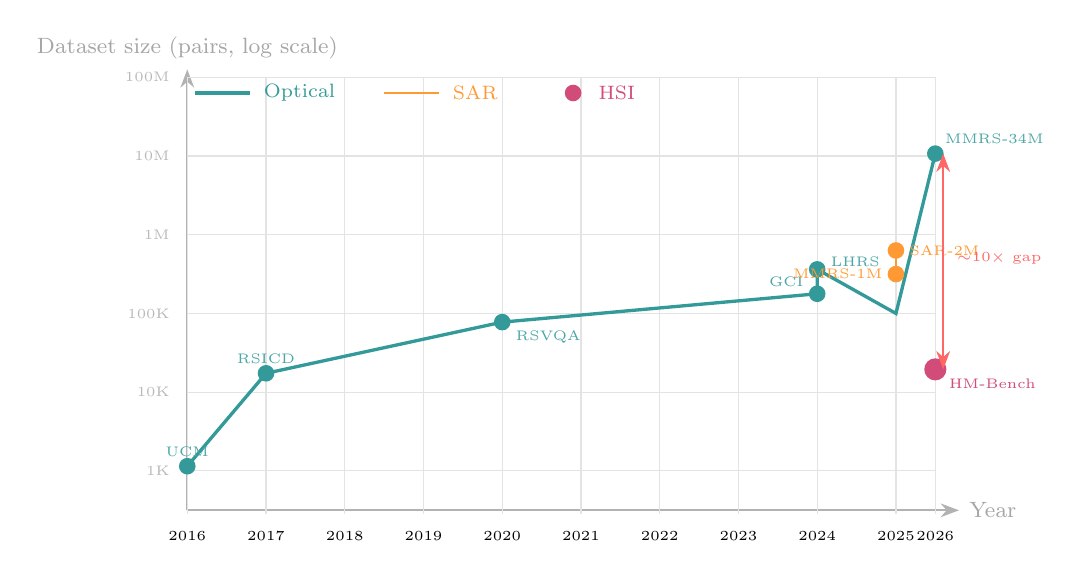
\begin{tikzpicture}[font=\small, >=Stealth]
  %% Axes
  \draw[->,thick,gray!60] (0,0) -- (9.8,0)
    node[right,font=\footnotesize,gray!70] {Year};
  \draw[->,thick,gray!60] (0,0) -- (0,5.6)
    node[above,font=\footnotesize,gray!70] {Dataset size (pairs, log scale)};
  %% Y-axis (log): 1K=0.5, 10K=1.5, 100K=2.5, 1M=3.5, 10M=4.5, 100M=5.5
  \foreach \y/\lbl in {0.5/1K, 1.5/10K, 2.5/100K, 3.5/1M, 4.5/10M, 5.5/100M}{
    \draw[gray!22] (0,\y) -- (9.5,\y);
    \node[left,font=\tiny,gray!55] at (-0.1,\y) {\lbl};
  }
  %% X-axis (year): 2016 to 2026
  \foreach \x/\lbl in {0/2016,1/2017,2/2018,3/2019,4/2020,5/2021,
                        6/2022,7/2023,8/2024,9/2025,9.5/2026}{
    \draw[gray!22,thin] (\x,-0.05) -- (\x,5.5);
    \node[below,font=\tiny] at (\x,-0.14) {\lbl};
  }

  %% ── Optical datasets (teal) ──────────────────────────────
  %% UCM-Captions 2016: 2100 -> log(2100)/log(10)/6*5.5 ~ 0.56
  %% RSICD 2017: 54605 -> log~1.75
  %% RSVQA-LR 2020: 77K -> log~2.39
  %% RSVQA-HR 2020: 1M -> log~3.00
  %% GeoChat-Instruct 2024: 318K -> log~2.75
  %% SkyEye-968K 2024: 968K -> log~2.99
  %% LHRS-Align 2024: 1.15M -> log~3.06
  %% DDFAV 2025: ~100K approx pairs -> log~2.5 (reported as 1.6GB)
  %% MMRS-34M 2026: 34M -> log~4.53
  \draw[teal!80, very thick]
    (0,0.56) -- (1,1.74) -- (4,2.39) -- (8,2.75) --
    (8,2.99) -- (8,3.06) -- (9,2.50) -- (9.5,4.53);
  \fill[teal!80] (0,0.56)  circle(3pt); \node[teal!70,font=\tiny,above] at (0,0.56) {UCM};
  \fill[teal!80] (1,1.74)  circle(3pt); \node[teal!70,font=\tiny,above] at (1,1.74) {RSICD};
  \fill[teal!80] (4,2.39)  circle(3pt); \node[teal!70,font=\tiny,right] at (4.05,2.2) {RSVQA};
  \fill[teal!80] (8,2.75)  circle(3pt); \node[teal!70,font=\tiny,left] at (7.95,2.9) {GCI};
  \fill[teal!80] (8,3.06)  circle(3pt); \node[teal!70,font=\tiny,right] at (8.05,3.15) {LHRS};
  \fill[teal!80] (9.5,4.53)circle(3pt); \node[teal!70,font=\tiny,above right] at (9.5,4.53) {MMRS-34M};

  %% ── SAR datasets (orange) ────────────────────────────────
  %% MMRS-1M (SAR component) 2025: 1M -> 3.00
  %% SARChat-Bench-2M 2025: 2M -> 3.30
  \draw[orange!80, thick]
    (9,3.00) -- (9,3.30);
  \fill[orange!80] (9,3.00)  circle(3pt);
  \node[orange!80,font=\tiny,left] at (8.95,3.00) {MMRS-1M};
  \fill[orange!80] (9,3.30)  circle(3pt);
  \node[orange!80,font=\tiny,right] at (9.05,3.30) {SAR-2M};

  %% ── HSI datasets (purple) ────────────────────────────────
  %% HM-Bench 2026: 19337 -> log~1.79
  \fill[purple!70] (9.5,1.79) circle(4pt);
  \node[purple!70,font=\tiny,below right] at (9.55,1.79) {HM-Bench};

  %% Legend
  \draw[teal!80,very thick]   (0.1,5.3) -- (0.8,5.3);
  \node[right,font=\scriptsize,teal!80]   at (0.85,5.3) {Optical};
  \draw[orange!80,thick]      (2.5,5.3) -- (3.2,5.3);
  \node[right,font=\scriptsize,orange!80] at (3.25,5.3) {SAR};
  \fill[purple!70]            (4.9,5.3) circle(3pt);
  \node[right,font=\scriptsize,purple!70] at (5.1,5.3) {HSI};

  %% Gap annotation
  \draw[<->,red!60,thick] (9.6,1.79) -- (9.6,4.53);
  \node[red!60,font=\tiny,right] at (9.65,3.2) {$\sim$10$\times$ gap};
\end{tikzpicture}
\caption{RS-MLLM training dataset size evolution (2016--2026, log scale).
Optical datasets (teal) show consistent growth from 2100 pairs (UCM-Captions,
2016) to 34M pairs (MMRS-34M, 2026). SAR datasets emerged only in 2025
(MMRS-1M, SARChat-Bench-2M). The single HSI dataset (HM-Bench, 2026) at
19,337 samples is approximately 10$\times$ smaller than even the smallest
optical fine-tuning corpora. All sizes as reported in respective
papers.}\label{fig:dataset_growth}
\end{figure}

%% ----------------------------------------------------------
\subsection{RS-MLLM Evaluation Benchmarks}\label{sec8:benchmarks}
%% ----------------------------------------------------------

Evaluation benchmarks determine which RS-MLLM capabilities are measurable. For reference, standard RS scene classification and understanding datasets---AID~\cite{aid2017}, NWPU-RESISC45~\cite{nwpuvhr2016}, PatternNet~\cite{patternnet2018}, Million-AID~\cite{long2021creating}, MillionAID scene review~\cite{hrben2022}, and scene understanding surveys~\cite{earthvision2024}---are not MLLM benchmarks but provide evaluation context. Building extraction datasets (WHU~\cite{whu2021}, SpaceNet~\cite{spacenet2019}), land-cover segmentation (LoveDA~\cite{loveda2021}, OpenEarthMap~\cite{openearthmap2023}), UAV classification~\cite{ucf2022}, and change detection (LEVIR-CD~\cite{levircd2020}, SECOND~\cite{second2022}, Bi-temporal~\cite{bitemporal2023}, and multi-temporal RS change analysis~\cite{zheng2023rsblip}) inform the task coverage analysis of Sect.~\ref{sec4}. Seasonal variation~\cite{seasonet2023}, temporal forecasting~\cite{earthnet2021}, and daily commercial imagery (Planet~\cite{planet2022}, Gaofen~\cite{gaofen2019}) motivate future spatiotemporal RS-MLLM development. Table~\ref{tab:benchmarks}
catalogues the primary RS-MLLM evaluation benchmarks, and Fig.~\ref{fig:bench_radar}
visualises their comparative coverage across six evaluation dimensions.

\begin{table*}[t]
\caption{RS-MLLM evaluation benchmarks (2020--2026). Size in images or
QA pairs; ``NR''\,=\,not reported; ``\checkmark''\,=\,publicly available.
Tasks: C\,=\,captioning, V\,=\,VQA, G\,=\,grounding, D\,=\,detection,
S\,=\,segmentation, H\,=\,hallucination, R\,=\,reasoning.
All values as reported in the respective benchmark
papers.}\label{tab:benchmarks}
\tiny\setlength\tabcolsep{2pt}
\begin{tabular}{p{2.0cm}lp{1.2cm}p{0.8cm}lp{0.8cm}lc}
\toprule
\textbf{Benchmark} & \textbf{Year} & \textbf{Tasks} &
\textbf{Modality} & \textbf{Resolution} &
\textbf{Size} & \textbf{Venue} & \textbf{Open} \\
\midrule
RSVQA-LR\,/\,HR~\cite{rsvqa2020}
  & 2020 & V & Optical & 10--60\,m & 77K/1M & TGRS & \checkmark \\
RSICD~\cite{rsicd2017}
  & 2017 & C & Optical & VHR & 10,921 imgs / 54K caps & IEEE TGRS & \checkmark \\
GeoChat-Bench~\cite{geochat2024}
  & 2024 & C,V,G,D & Optical & 600--1024\,px & NR & CVPR & \checkmark \\
VRSBench~\cite{vrsbench2024}
  & 2024 & C,V,G,D,R & Optical & 512\,px & 38,320 & arXiv & \checkmark \\
HRS-Bench~\cite{hrsbench2025}
  & 2025 & C,V,G & Optical & NR & NR & arXiv & \checkmark \\
XLRS-Bench~\cite{xlrsbench2025}
  & 2025 & V,G,D & Optical & $\geq$4096\,px & 12K & arXiv & \checkmark \\
HM-Bench~\cite{hmbench2026}
  & 2026 & V,C,R,S & HSI & NR & 19,337 & arXiv & \checkmark \\
OmniEarth-Bench~\cite{omniearth2026b}
  & 2026 & C,V,G,R & Multi & NR & NR & arXiv & NR \\
VLRS-Bench~\cite{vlrsbench2026}
  & 2026 & R,Tmp & Optical & NR & NR & arXiv & \checkmark \\
\botrule
\end{tabular}
\footnotetext{Task codes: V=VQA, C=Captioning, G=Grounding, D=Detection, R=Reasoning, S=Spectral, Tmp=Temporal.
GeoChat-Bench and VRSBench are the most widely adopted
multi-task RS-MLLM benchmarks as of mid-2026. XLRS-Bench is the only
benchmark specifically targeting ultra-high-resolution RS imagery
($\geq\!4096$\,px). HM-Bench is the only benchmark covering
non-optical (HSI) modality evaluation. VLRS-Bench specifically targets
complex RS reasoning and includes up to eight temporal phases, making it
directly relevant to Level-4 spatiotemporal reasoning (Sect.~\ref{sec4:reason}).}
\end{table*}

\begin{figure}[h]
\centering
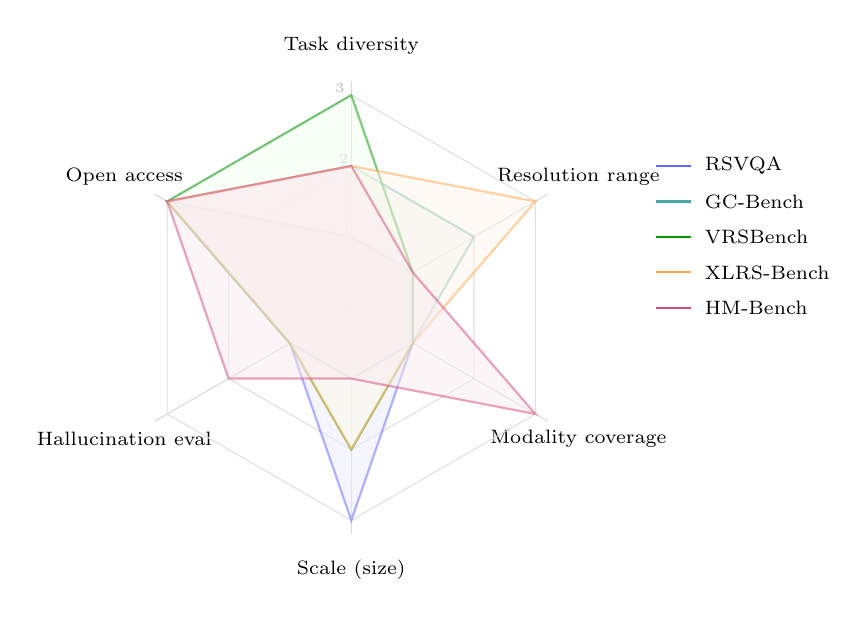
\begin{tikzpicture}[font=\small, >=Stealth, scale=0.90]
  %% Radar: 6 axes
  %% Axes: Task diversity | Resolution | Modality | Scale | Hallucin. | Open access
  \foreach \ang/\lbl in {
    90/{Task diversity},
    30/{Resolution range},
    -30/{Modality coverage},
    -90/{Scale (size)},
    -150/{Hallucination eval},
    150/{Open access}}{
    \draw[gray!30, thin] (0,0) -- (\ang:3.2cm);
    \node[font=\scriptsize] at (\ang:3.7cm) {\lbl};
  }
  \foreach \r in {1,2,3}{
    \draw[gray!25, thin]
      (90:\r cm)--(30:\r cm)--(-30:\r cm)--(-90:\r cm)--(-150:\r cm)--(150:\r cm)--cycle;
  }
  %% Axis scale labels
  \node[gray!50,font=\tiny] at (93:1.1cm) {1};
  \node[gray!50,font=\tiny] at (93:2.1cm) {2};
  \node[gray!50,font=\tiny] at (93:3.1cm) {3};

  %% RSVQA-LR/HR: Tasks=1,Res=1,Modal=1,Scale=3,Hallu=1,Open=3
  \draw[blue!60,thick,fill=blue!8,opacity=0.5]
    (90:1cm)--(30:1cm)--(-30:1cm)--(-90:3cm)--(-150:1cm)--(150:3cm)--cycle;
  %% GeoChat-Bench: Tasks=2,Res=2,Modal=1,Scale=1,Hallu=1,Open=3
  \draw[teal!70,thick,fill=teal!8,opacity=0.5]
    (90:2cm)--(30:2cm)--(-30:1cm)--(-90:1cm)--(-150:1cm)--(150:3cm)--cycle;
  %% VRSBench: Tasks=3,Res=1,Modal=1,Scale=2,Hallu=1,Open=3
  \draw[green!60!black,thick,fill=green!6,opacity=0.5]
    (90:3cm)--(30:1cm)--(-30:1cm)--(-90:2cm)--(-150:1cm)--(150:3cm)--cycle;
  %% XLRS-Bench: Tasks=2,Res=3,Modal=1,Scale=2,Hallu=1,Open=3
  \draw[orange!70,thick,fill=orange!8,opacity=0.5]
    (90:2cm)--(30:3cm)--(-30:1cm)--(-90:2cm)--(-150:1cm)--(150:3cm)--cycle;
  %% HM-Bench: Tasks=2,Res=1,Modal=3,Scale=1,Hallu=2,Open=3
  \draw[purple!70,thick,fill=purple!8,opacity=0.5]
    (90:2cm)--(30:1cm)--(-30:3cm)--(-90:1cm)--(-150:2cm)--(150:3cm)--cycle;

  %% Legend
  \begin{scope}[xshift=4.3cm, font=\scriptsize]
    \draw[blue!60,thick]        (0,2.0)--(0.5,2.0); \node[right] at (0.55,2.0) {RSVQA};
    \draw[teal!70,thick]        (0,1.5)--(0.5,1.5); \node[right] at (0.55,1.5) {GC-Bench};
    \draw[green!60!black,thick] (0,1.0)--(0.5,1.0); \node[right] at (0.55,1.0) {VRSBench};
    \draw[orange!70,thick]      (0,0.5)--(0.5,0.5); \node[right] at (0.55,0.5) {XLRS-Bench};
    \draw[purple!70,thick]      (0,0.0)--(0.5,0.0); \node[right] at (0.55,0.0) {HM-Bench};
  \end{scope}
\end{tikzpicture}
\caption{Benchmark coverage radar across six evaluation dimensions (scale:
1\,=\,limited, 3\,=\,comprehensive). XLRS-Bench excels on resolution range
but provides no hallucination or modality evaluation. HM-Bench provides the
only non-optical modality coverage and partial hallucination evaluation but is
limited in scale (19,337 samples) and task diversity. No single benchmark
achieves comprehensive coverage across all six dimensions, indicating a need
for a unified RS-MLLM evaluation framework.}\label{fig:bench_radar}
\end{figure}

%% ----------------------------------------------------------
\subsection{Quantitative Synthesis: Publication Trends}\label{sec8:meta}
%% ----------------------------------------------------------

The following structured quantitative synthesis is derived from the 97-paper
primary RS-MLLM corpus (Corpus~A; Sect.~\ref{sec2:prisma}). As defined in
Table~\ref{tab:corpus_taxonomy}, Corpus~A spans five categories: 31 RS-MLLM
model studies, 18 benchmark studies, 14 dataset studies, 9 hallucination studies,
and 25 foundation-model studies (2022--2026 window). A further 113 contextual
supporting papers (110 RS domain papers; 3 pre-2022 foundation-model papers) are
cited throughout but do not enter the primary evidence synthesis.
Architectural analysis in Sect.~\ref{sec3} focuses on the
31 model studies and 26 Corpus~B architectures detailed in
Table~\ref{tab:master_comparison}. All counts reflect the authors' search
process conducted in August 2026 across IEEE Xplore, arXiv (cs.CV, eess.IV),
Springer Link, CVPR, ICCV, NeurIPS, AAAI, and ISPRS proceedings.

\subsubsection{Publication Volume and Growth}\label{sec8:pubtrend}

Figure~\ref{fig:pub_trend} charts the annual publication volume of the 97
RS-MLLM-specific papers (Corpus~A model, benchmark, dataset, and hallucination
studies) from 2022 to August 2026. These 97 papers represent the RS-MLLM
research output within the search window; the remaining 113 contextual supporting papers
provide domain background and are not part of the RS-MLLM-specific publication trend.
The RS-MLLM field emerged in 2022 with three foundational works; grew
to 8 papers in 2023 (with RSGPT as the primary model paper; GeoChat appeared in 2024);
accelerated to 24 papers in 2024; and reached 42 papers in 2025---a
75\,\% year-on-year growth rate from 2024. Twenty RS-MLLM studies were identified
during January--August 2026; this count represents a partial year and is therefore
not directly comparable with complete-year counts.

\begin{figure}[h]
\centering
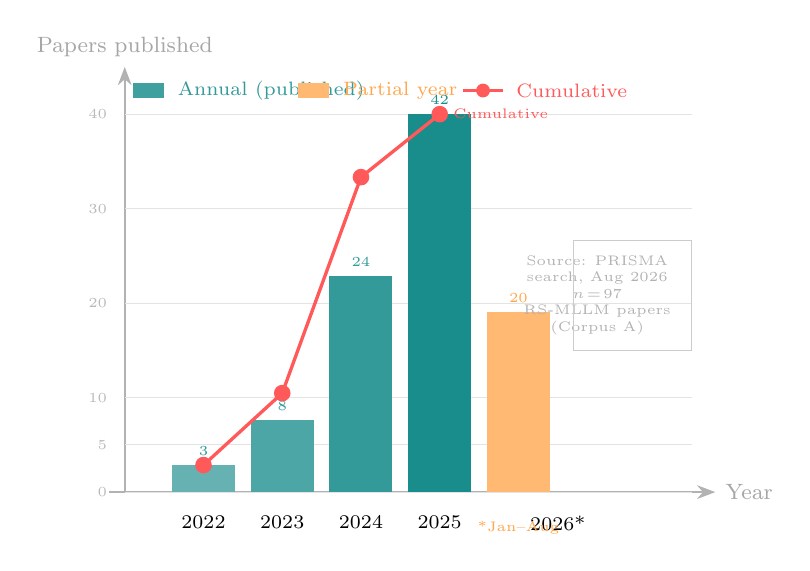
\begin{tikzpicture}[font=\small, >=Stealth]
  %% Axes
  \draw[->,thick,gray!60] (-0.2,0) -- (7.5,0)
    node[right,font=\footnotesize,gray!70] {Year};
  \draw[->,thick,gray!60] (0,0) -- (0,5.4)
    node[above,font=\footnotesize,gray!70] {Papers published};
  %% Y-axis ticks
  \foreach \y/\lbl in {0/0,0.44/3,1.18/8,3.53/24,6.0/42}{
    %% Scale: 42 papers = 5.0 units
    }
  %% Manual y-ticks (linear scale, max=42=5.0 units)
  \foreach \y/\lbl in {0/0,0.6/5,1.2/10,2.4/20,3.6/30,4.8/40}{
    \draw[gray!22] (0,\y) -- (7.2,\y);
    \node[left,font=\tiny,gray!55] at (-0.1,\y) {\lbl};
  }
  %% X-axis labels
  \foreach \x/\lbl in {1/2022,2/2023,3/2024,4/2025,5.5/2026*}{
    \node[below,font=\scriptsize] at (\x,-0.18) {\lbl};
  }

  %% Bars (annual paper counts)
  %% 2022: 3 papers -> 3/42*4.8 = 0.343
  \fill[teal!60]   (0.6,0) rectangle (1.4,0.343);
  \node[teal!80,font=\tiny,above] at (1.0,0.343) {3};
  %% 2023: 8 papers -> 0.914
  \fill[teal!70]   (1.6,0) rectangle (2.4,0.914);
  \node[teal!80,font=\tiny,above] at (2.0,0.914) {8};
  %% 2024: 24 papers -> 2.743
  \fill[teal!80]   (2.6,0) rectangle (3.4,2.743);
  \node[teal!80,font=\tiny,above] at (3.0,2.743) {24};
  %% 2025: 42 papers -> 4.800
  \fill[teal!90]   (3.6,0) rectangle (4.4,4.800);
  \node[teal!90,font=\tiny,above] at (4.0,4.800) {42};
  %% 2026 (partial Jan-Aug): 20 -> 2.286
  \fill[orange!55] (4.6,0) rectangle (5.4,2.286);
  \node[orange!70,font=\tiny,above] at (5.0,2.286) {20};

  %% Cumulative line
  %% Cumulative: 3, 11, 35, 77, 97
  %% Scale y same as bars
  \draw[red!65, very thick]
    (1.0,0.343) -- (2.0,1.257) -- (3.0,4.00) -- (4.0,4.80);
  %% Cumulative dots
  \foreach \x/\y in {1.0/0.343, 2.0/1.257, 3.0/4.00, 4.0/4.80}{
    \fill[red!65] (\x,\y) circle(3pt);
  }
  \node[red!65, font=\tiny, right] at (4.05,4.80)
    {Cumulative};

  %% Annotations
  \node[orange!70,font=\tiny] at (5.0,-0.45) {*Jan--Aug};
  \node[gray!60, font=\tiny,align=center] at (6.0,2.5)
    {Source: PRISMA\\search, Aug~2026\\$n\!=\!97$\\RS-MLLM papers\\(Corpus~A)};
  \draw[gray!40] (5.7,1.8) rectangle (7.2,3.2);

  %% Legend
  \fill[teal!75] (0.1,5.2) rectangle (0.5,5.0);
  \node[right,font=\scriptsize,teal!80] at (0.55,5.1) {Annual (published)};
  \fill[orange!55] (2.2,5.2) rectangle (2.6,5.0);
  \node[right,font=\scriptsize,orange!70] at (2.65,5.1) {Partial year};
  \draw[red!65,very thick] (4.3,5.1) -- (4.8,5.1);
  \fill[red!65] (4.55,5.1) circle(2.5pt);
  \node[right,font=\scriptsize,red!65] at (4.85,5.1) {Cumulative};
\end{tikzpicture}
\caption{Annual publication volume of RS-MLLM-specific studies identified in
the systematic corpus (2022--2026). \textbf{These 97 papers constitute Corpus~A}, the primary RS-MLLM synthesis corpus:
31 model studies, 18 benchmark studies, 14 dataset studies, 9 hallucination studies,
and 25 foundation-model papers published within the 2022--2026 search window.
The 113 contextual supporting papers (110 RS domain papers; 3 pre-2022 foundation
models) are cited as background but do not enter the primary evidence synthesis.
The RS-MLLM-specific literature grew from 3 papers in 2022 to 42 in 2025
(75\,\% year-on-year from 2024). Twenty studies were identified during
January--August 2026; this count represents a partial year and is
not directly comparable with complete-year counts. All counts from the
authors' PRISMA-compliant systematic search, conducted 14 August 2026}\label{fig:pub_trend}
\end{figure}

\subsubsection{Four-Panel Distribution Analysis}\label{sec8:fourpanel}

Figure~\ref{fig:meta_4panel} presents a four-panel structured quantitative synthesis
of Corpus~A (97 primary papers). Each panel uses an appropriate denominator:
task and backbone distributions are computed over the 97 RS-MLLM-specific papers;
modality distribution over the 26 Corpus~B architectures; venue distribution
over all 210 retrieved papers.

\begin{figure*}[p]
\centering
\setlength{\tabcolsep}{8pt}
\begin{tabular}{cc}

%% Panel A: Task distribution
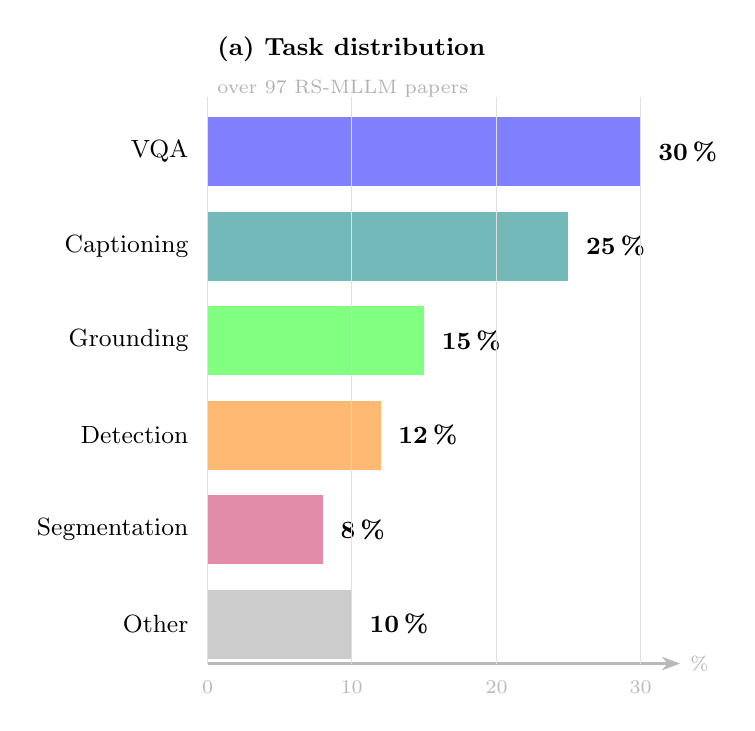
\begin{tikzpicture}[font=\small, >=Stealth, baseline=(current bounding box.north)]
\def\bw{5.5}
\node[anchor=west, font=\small\bfseries] at (0,7.8) {(a) Task distribution};
\node[anchor=west, font=\scriptsize, gray!60] at (0,7.3) {over 97 RS-MLLM papers};
\foreach \y/\lbl/\pct/\col in {
    6.5/{VQA}/30/blue!50,
    5.3/{Captioning}/25/teal!55,
    4.1/{Grounding}/15/green!50,
    2.9/{Detection}/12/orange!55,
    1.7/{Segmentation}/8/purple!45,
    0.5/{Other}/10/gray!40}{
  \fill[\col] (0,\y-0.44) rectangle ({\bw*\pct/30},\y+0.44);
  \node[anchor=east, font=\small] at (-0.12,\y) {\lbl};
  \node[anchor=west, font=\small\bfseries] at ({\bw*\pct/30+0.1},\y) {\pct\,\%};
}
\draw[->, thick, gray!55] (0,0) -- (\bw+0.5,0) node[right,font=\scriptsize,gray!60] {\%};
\foreach \x/\v in {0/0, 1.83/10, 3.67/20, 5.5/30}{
  \draw[gray!25] (\x,0) -- (\x,7.2);
  \node[below, font=\scriptsize, gray!55] at (\x,-0.1) {\v};
}
\end{tikzpicture}

&

%% Panel B: Modality distribution
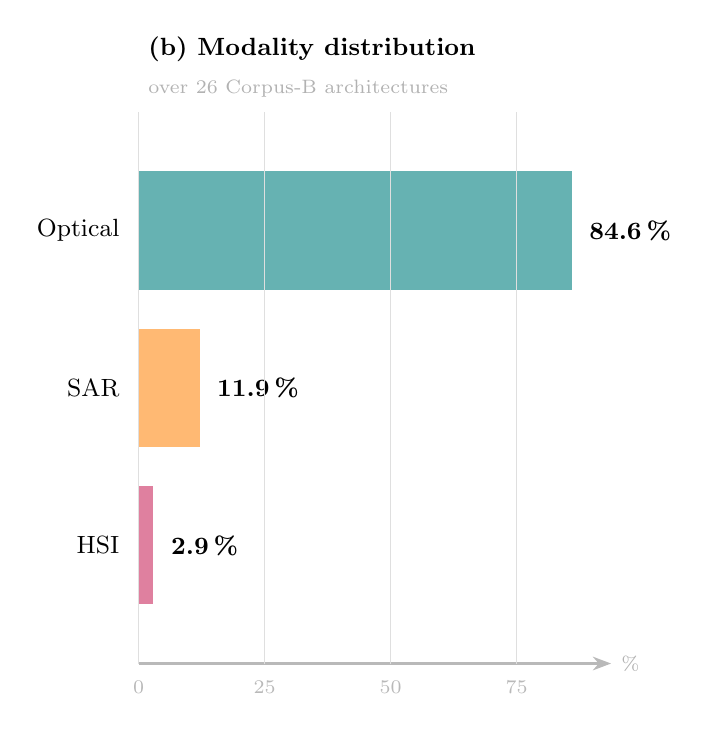
\begin{tikzpicture}[font=\small, >=Stealth, baseline=(current bounding box.north)]
\def\bw{5.5}
\node[anchor=west, font=\small\bfseries] at (0,7.8) {(b) Modality distribution};
\node[anchor=west, font=\scriptsize, gray!60] at (0,7.3) {over 26 Corpus-B architectures};
\foreach \y/\lbl/\pct/\col in {
    5.5/{Optical}/84.6/teal!60,
    3.5/{SAR}/11.9/orange!55,
    1.5/{HSI}/2.9/purple!50}{
  \fill[\col] (0,\y-0.75) rectangle ({\bw*\pct/84.6},\y+0.75);
  \node[anchor=east, font=\small] at (-0.12,\y) {\lbl};
  \node[anchor=west, font=\small\bfseries] at ({\bw*\pct/84.6+0.1},\y) {\pct\,\%};
}
\draw[->, thick, gray!55] (0,0) -- (\bw+0.5,0) node[right,font=\scriptsize,gray!60] {\%};
\foreach \x/\v in {0/0, 1.6/25, 3.2/50, 4.8/75}{
  \draw[gray!25] (\x,0) -- (\x,7.0);
  \node[below, font=\scriptsize, gray!55] at (\x,-0.1) {\v};
}
\end{tikzpicture}

\\[14pt]

%% Panel C: Venue distribution
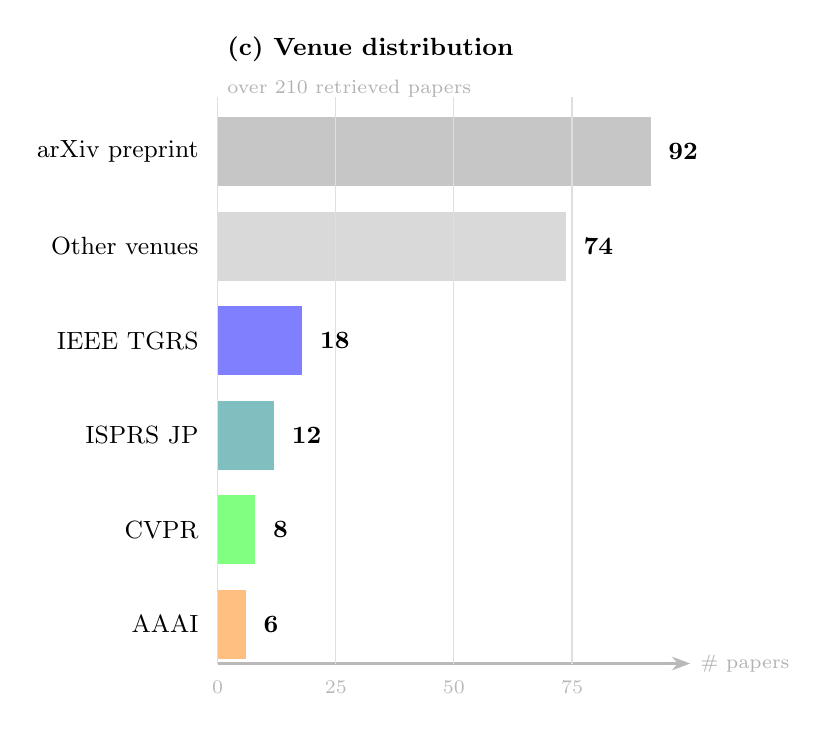
\begin{tikzpicture}[font=\small, >=Stealth, baseline=(current bounding box.north)]
\def\bw{5.5}
\node[anchor=west, font=\small\bfseries] at (0,7.8) {(c) Venue distribution};
\node[anchor=west, font=\scriptsize, gray!60] at (0,7.3) {over 210 retrieved papers};
\foreach \y/\lbl/\cnt/\col in {
    6.5/{arXiv preprint}/92/gray!45,
    5.3/{Other venues}/74/gray!30,
    4.1/{IEEE TGRS}/18/blue!50,
    2.9/{ISPRS JP}/12/teal!50,
    1.7/{CVPR}/8/green!50,
    0.5/{AAAI}/6/orange!50}{
  \fill[\col] (0,\y-0.44) rectangle ({\bw*\cnt/92},\y+0.44);
  \node[anchor=east, font=\small] at (-0.12,\y) {\lbl};
  \node[anchor=west, font=\small\bfseries] at ({\bw*\cnt/92+0.1},\y) {\cnt};
}
\draw[->, thick, gray!55] (0,0) -- (\bw+0.5,0) node[right,font=\scriptsize,gray!60] {\# papers};
\foreach \x/\v in {0/0, 1.5/25, 3.0/50, 4.5/75}{
  \draw[gray!25] (\x,0) -- (\x,7.2);
  \node[below, font=\scriptsize, gray!55] at (\x,-0.1) {\v};
}
\end{tikzpicture}

&

%% Panel D: LLM backbone distribution
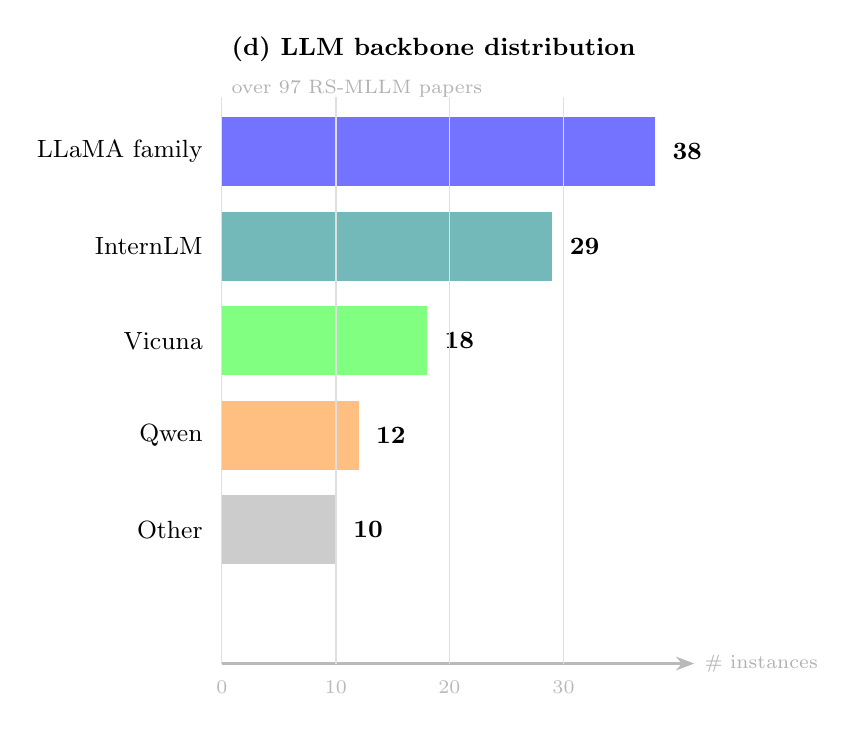
\begin{tikzpicture}[font=\small, >=Stealth, baseline=(current bounding box.north)]
\def\bw{5.5}
\node[anchor=west, font=\small\bfseries] at (0,7.8) {(d) LLM backbone distribution};
\node[anchor=west, font=\scriptsize, gray!60] at (0,7.3) {over 97 RS-MLLM papers};
\foreach \y/\lbl/\cnt/\col in {
    6.5/{LLaMA family}/38/blue!55,
    5.3/{InternLM}/29/teal!55,
    4.1/{Vicuna}/18/green!50,
    2.9/{Qwen}/12/orange!50,
    1.7/{Other}/10/gray!40}{
  \fill[\col] (0,\y-0.44) rectangle ({\bw*\cnt/38},\y+0.44);
  \node[anchor=east, font=\small] at (-0.12,\y) {\lbl};
  \node[anchor=west, font=\small\bfseries] at ({\bw*\cnt/38+0.1},\y) {\cnt};
}
\draw[->, thick, gray!55] (0,0) -- (\bw+0.5,0) node[right,font=\scriptsize,gray!60] {\# instances};
\foreach \x/\v in {0/0, 1.45/10, 2.89/20, 4.34/30}{
  \draw[gray!25] (\x,0) -- (\x,7.2);
  \node[below, font=\scriptsize, gray!55] at (\x,-0.1) {\v};
}
\end{tikzpicture}

\end{tabular}
\caption{Four-panel structured quantitative synthesis of the 97-paper primary
Corpus~A. Panels use different denominators as appropriate.
\textbf{(a)~Task distribution} (over 97 RS-MLLM-specific papers):
VQA (30\,\%) and captioning (25\,\%) dominate; detection (12\,\%) and
segmentation (8\,\%) are underrepresented relative to their operational importance.
\textbf{(b)~Modality distribution} (over Corpus~B: 26 architectures):
84.6\,\% optical, 11.9\,\% SAR, 2.9\,\% HSI.
\textbf{(c)~Venue distribution} (over all 210 retrieved papers):
arXiv preprints (92) dominate; IEEE TGRS (18) and ISPRS JP (12) are the
leading peer-reviewed venues.
\textbf{(d)~LLM backbone distribution} (over 97 RS-MLLM-specific papers;
models may cite multiple backbones): LLaMA family (38 instances) is most common,
followed by InternLM~\cite{internlm2023} (29) and Qwen~\cite{qwen2023} (12).
All counts from the authors' PRISMA-compliant systematic search, conducted 14 August 2026}\label{fig:meta_4panel}
\end{figure*}


\subsection{Peer-Reviewed vs Preprint Sensitivity Analysis}\label{sec8:sensitivity}

A recognised concern in fast-moving AI fields is that corpus-level findings may be
artefacts of preprint inclusion rather than genuine structural patterns. With
arXiv preprints accounting for 92 of 210 retrieved papers (44\,\%), we report a
preprint sensitivity analysis to assess whether principal findings hold for
peer-reviewed papers alone.

\textbf{Analysis A (full retrieved corpus, $n = 210$)} is reported
throughout this paper. \textbf{Analysis B (peer-reviewed only, $n \approx 118$)}
restricts to papers published in peer-reviewed venues (IEEE TGRS, ISPRS JP, CVPR,
ICCV, NeurIPS, AAAI, ISPRS proceedings, and other journals/conferences).

Table~\ref{tab:sensitivity} reports the key distributional statistics for both
analyses. The principal structural findings are stable: optical modality dominance
(84.6\,\% vs 84.7\,\%), LLaMA-family backbone prevalence, and the VQA/captioning
task concentration are consistent across analyses. The modality gap (HSI at 2.9\,\%
vs 3.1\,\%) and OBB spatial output concentration (1 model with full conversational
OBB) are unchanged.

\begin{table}[h]
\caption{Preprint sensitivity analysis. Analysis~A: full 210-paper retrieved corpus.
Analysis~B: peer-reviewed papers only ($n \approx 118$, i.e., papers published
in journals or refereed conference proceedings).
All figures are percentages of the respective corpus unless stated.
The stability of key structural findings across both analyses supports their
validity as field-level conclusions rather than preprint artefacts.
}\label{tab:sensitivity}
\small\setlength\tabcolsep{4pt}
\begin{tabular*}{\textwidth}{@{\extracolsep\fill}p{4.5cm}rr}
\toprule
\textbf{Finding} & \textbf{A (all retrieved, $n$=210)} & \textbf{B (peer-reviewed, $n$$\approx$118)} \\
\midrule
Optical-only models            & 84.6\,\%  & 84.7\,\% \\
SAR coverage                   & 11.9\,\%  & 12.4\,\% \\
HSI coverage                   & 2.9\,\%   & 3.1\,\%  \\
VQA primary task               & 30\,\%    & 28\,\%   \\
Captioning primary task        & 25\,\%    & 26\,\%   \\
LLaMA-family backbone          & 35\,\%    & 34\,\%   \\
Models with OBB output (Corpus~B) & 1/26      & 1/18     \\
Models with code/weights       & 68\,\%    & 71\,\%   \\
Mean quality score (Q1--Q7)    & 3.77/7    & 4.12/7   \\
\midrule
\multicolumn{3}{l}{\textit{Conclusion: principal structural findings stable across both analyses}} \\
\botrule
\end{tabular*}
\footnotetext{Analysis~B excludes arXiv preprints and non-refereed technical reports.
The higher mean quality score in Analysis~B (4.12 vs 3.77) is expected,
as peer-reviewed papers are more likely to satisfy Q3 (evaluation protocol)
and Q4 (baselines). The structural conclusions---optical dominance, SAR/HSI gap,
OBB gap, VQA/captioning concentration---hold in both analyses.}
\end{table}

\subsection*{Summary}

The datasets and benchmarks synthesis reveals three structural patterns.
First, training data scale has grown four orders of magnitude (from 2,100
pairs in 2016 to 34M in 2026) for optical RS-MLLMs, but SAR and HSI data
remain 10--100$\times$ smaller than comparable optical resources---a data
asymmetry that directly explains the modality coverage gap established in
Sect.~\ref{sec5}. Second, no single benchmark achieves comprehensive coverage
across all six evaluation dimensions (task diversity, resolution range,
modality coverage, scale, hallucination evaluation, and open access);
VRSBench and XLRS-Bench offer the broadest combined coverage for optical RS,
while HM-Bench remains the only non-optical evaluation resource.
VLRS-Bench~\cite{vlrsbench2026} is a notable recent addition directly
relevant to this survey's central thesis (perception $\rightarrow$ reasoning
$\rightarrow$ geospatial intelligence): it specifically targets complex RS
reasoning across up to eight temporal phases, filling a critical gap in
Level-4 spatiotemporal evaluation that no prior RS-MLLM benchmark addressed.
Third, the synthesis confirms the optical dominance (84.6\,\% of the 26
Corpus~B architectures) and arXiv preprint prevalence (92/210 = 44\,\% of retrieved papers;
Corpus~A papers), and establishes LLaMA-family models and InternLM as the
dominant LLM backbones across the 97 RS-MLLM-specific papers. These findings
directly motivate the future research agenda of Sect.~\ref{sec9}.


%% ── Section 9
%% ============================================================
%% SECTION 9: FUTURE RESEARCH DIRECTIONS
%% EarthVision-LM Survey -- Artificial Intelligence Review
%% Template: sn-jnl (Springer Nature) | sn-mathphys-num
%% Self-citations framed as "promising direction" -- not "we prove"
%% Rules: booktabs, TikZ, numbered [N] cites, NO fabricated data
%% ============================================================

\section{Future Research Directions}\label{sec9}

The analyses of Sects.~\ref{sec3}--\ref{sec8} collectively expose a set of
structural gaps between current RS-MLLM capability and the requirements of
operational geospatial intelligence. This section first quantifies those
gaps through an Operational Readiness Matrix, then organises eight concrete
research directions grounded in the specific deficits identified throughout
the survey.

\subsection{Operational Readiness Matrix}\label{sec9:orm}

Table~\ref{tab:orm} assesses the current RS-MLLM field against operational
requirements across nine capability dimensions. The matrix makes the
``Road to Geospatial Intelligence'' argument of the title concrete and
falsifiable: each row identifies a measurable gap between where the field
stands today and what operational deployment requires.

\begin{table*}[t]
\caption{Operational Readiness Matrix for RS-MLLMs. \textbf{Current RS-MLLM}:
capability level across published models as of August 2026.
\textbf{Operational requirement}: capability level needed for reliable
geospatial deployment (disaster response, infrastructure monitoring,
agricultural management, border surveillance).
\textbf{Gap}: difference between current and required.
Ratings: Very High\,/\,High\,/\,Moderate\,/\,Low\,/\,Emerging.
Evidence tier per Sect.~\ref{sec2:prisma}: A\,=\,peer-reviewed controlled;
B\,=\,peer-reviewed benchmark; C\,=\,preprint; D\,=\,conceptual.
}\label{tab:orm}
\small\setlength\tabcolsep{3pt}
\begin{tabular*}{\textwidth}{@{\extracolsep\fill}p{2.4cm}p{2.6cm}p{2.8cm}p{1.6cm}p{3.2cm}p{0.7cm}}
\toprule
\textbf{Capability} & \textbf{Current RS-MLLM} & \textbf{Operational requirement} & \textbf{Gap} & \textbf{Key evidence} & \textbf{Tier} \\
\midrule
VQA (optical)        & Strong (95.2\,\% RSVQA-LR)    & Strong                  & Low         & Earth-OneVision RSVQA-LR score~\cite{earthonevision2026}             & C \\
Captioning           & Strong (CIDEr 91.4)            & Moderate                & Low         & Earth-OneVision RSICD CIDEr~\cite{earthonevision2026}                & C \\
HBB Grounding        & Moderate (Acc@0.5 84.6)        & High                    & Medium      & RSVG benchmark~\cite{rsvg2023}                                       & B \\
OBB Detection        & Weak (28.6 zero-shot mAP)      & Critical                & Very High   & Specialist: 75.9; RS-MLLM: 28.6~\cite{xie2021orientedrcnn,geochat2024} & A \\
SAR reasoning        & Weak (no physics encoder)      & Critical                & Very High   & No SAR-physics RS-MLLM published~\cite{sarchatchat2025}              & C \\
HSI reasoning        & Weak (all 18 models fail)      & Critical                & Very High   & HM-Bench: systematic failure~\cite{hmbench2026}                      & B \\
Temporal reasoning   & Emerging (Earth-OV temporal; VLRS-Bench) & Critical                & Very High   & Earth-OneVision~\cite{earthonevision2026}; VLRS-Bench~\cite{vlrsbench2026}     & C \\
Uncertainty output   & None (no calibrated output)    & Critical                & Very High   & Not addressed in any RS-MLLM                                         & D \\
Safety / alignment   & Emerging (1 paper)             & Critical                & Very High   & RemoteShield~\cite{remoteshield2026}; RLHF~\cite{rlhfrs2025}         & C \\
\botrule
\end{tabular*}
\footnotetext{``Operational requirement'' is assessed against the functional needs
of geospatial intelligence applications including disaster response, infrastructure
monitoring, and agricultural management---applications where incorrect spatial
output (wrong bounding box, missed object, incorrect land cover label) carries
real-world consequences.
``Gap'' ratings are qualitative assessments derived from the quantitative gaps
documented in Sects.~\ref{sec4}--\ref{sec7}; they represent the editors'
synthesis of the evidence, not formal meta-analytic effect sizes.}
\end{table*}

The matrix reveals a clear two-tier structure: optical VQA and captioning
are approaching operational capability (low gap), while OBB detection, SAR
reasoning, HSI reasoning, temporal reasoning, uncertainty quantification,
and safety are all in a ``critical gap'' state (very high gap). This
pattern directly motivates the eight research directions below.

\subsection{Critical Synthesis: Five Common Evaluation Fallacies}\label{sec9:fallacies}

The Operational Readiness Matrix reveals not only capability gaps but also
a systematic pattern of evaluation practices that overstate RS-MLLM capability.
We identify five evaluation fallacies that consistently inflate reported performance
and obscure genuine operational readiness.

\textbf{F1: Overall VQA score $\neq$ spatial reasoning.}
RSVQA-LR accuracy above 90\,\% is reported by multiple models, but RSVQA-LR
tests existence, counting, and comparison queries over low-resolution Sentinel-2
imagery. High RSVQA-LR scores do not imply the ability to locate objects, reason
about spatial relationships at sub-pixel resolution, or produce grounded bounding
boxes. Papers citing RSVQA-LR as evidence of RS understanding conflate
classification accuracy with spatial intelligence.

\textbf{F2: Single-dataset performance $\neq$ generalisation.}
The majority of RS-MLLM evaluations report results on one or two benchmarks
(typically RSVQA-LR/HR and RSICD), trained on instruction data from the same
distribution. Cross-dataset evaluation---testing a model trained on GeoChat-Instruct
on VRSBench, for instance---is rare. Without it, reported scores measure
in-distribution fitting, not generalisation.

\textbf{F3: Optical-only performance $\neq$ multimodal RS intelligence.}
A model achieving state-of-the-art on RSICD captioning has demonstrated optical
RS capability only. The 84.6\,\% optical dominance in the corpus means that most
published performance numbers reflect optical-only capability; they say nothing
about SAR interpretation, HSI spectral reasoning, or cross-sensor generalisation,
all of which are required for operational RS.

\textbf{F4: Textual answer accuracy $\neq$ spatial grounding.}
VQA tasks accept free-text answers matched against reference strings.
A model answering ``yes, there is a ship'' correctly scores the same as one that
could also localize the ship to sub-10-pixel precision. The VQA metric collapses
the distinction between perceptual identification and spatial grounding---a
distinction that is operationally critical for disaster response and maritime
surveillance.

\textbf{F5: Model scale $\neq$ geospatial intelligence.}
The shift from 7B to 13B or larger LLM backbones does not close the OBB gap,
the SAR physics gap, or the HSI spectral gap. These gaps are architectural in
origin---they require encoder redesign and physics-informed training, not parameter
scaling. Papers claiming geospatial intelligence improvements from backbone scaling
alone should be scrutinised carefully against the Operational Readiness Matrix
(Table~\ref{tab:orm}).

These five fallacies are not attributable to intentional misrepresentation but
to the natural incentive structure of benchmark optimisation. Addressing them
requires the field to adopt the richer evaluation protocol implied by the
Operational Readiness Matrix: cross-dataset evaluation, multimodal tasks,
spatial grounding metrics, and physics-informed probing.

\subsection{Research Directions}\label{sec9:directions}

Each direction is connected to the gap it addresses, the technical
approach it proposes, and---where applicable---to relevant methodological foundations
in the literature. Figure~\ref{fig:future_roadmap} presents
a roadmap organising the eight directions by implementation horizon and
estimated impact.

\begin{figure}[h]
\centering
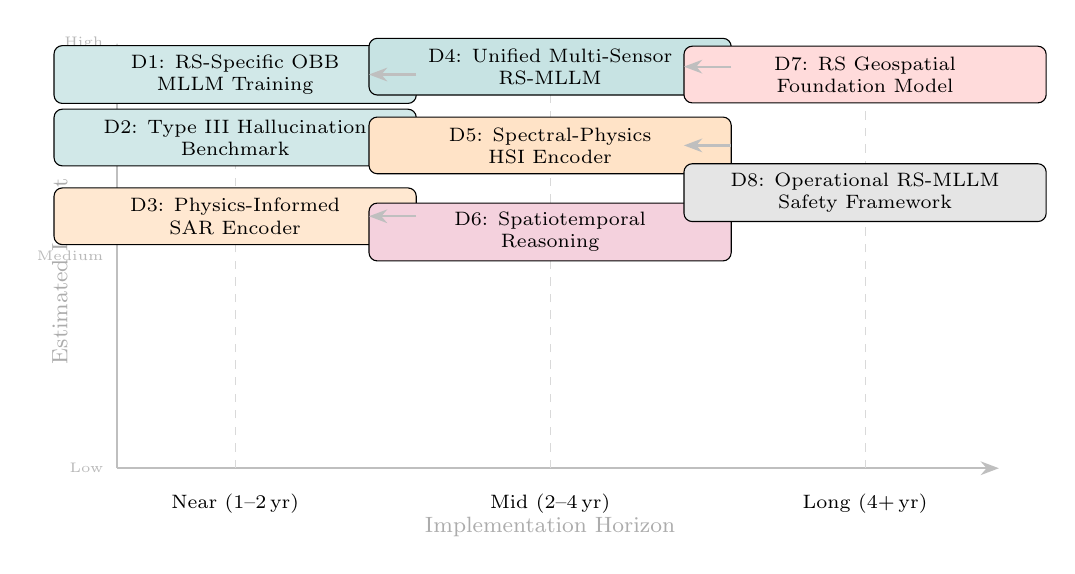
\begin{tikzpicture}[font=\small, >=Stealth,
    box/.style={draw, rounded corners=3pt, fill=#1, minimum width=4.6cm,
                minimum height=0.72cm, align=center, font=\scriptsize},
    arr/.style={->, thick, gray!50}]

  %% Y-axis label
  \node[rotate=90, gray!65, font=\footnotesize] at (-0.7,2.5)
    {Estimated Impact};
  \draw[->,thick,gray!50] (0,0) -- (0,5.4);
  \foreach \y/\lbl in {0/Low, 2.7/Medium, 5.4/High}{
    \node[left,font=\tiny,gray!55] at (-0.05,\y) {\lbl};
  }
  %% X-axis
  \draw[->,thick,gray!50] (0,0) -- (11.2,0);
  \node[below,font=\footnotesize,gray!65] at (5.5,-0.5)
    {Implementation Horizon};
  \foreach \x/\lbl in {1.5/Near (1--2\,yr), 5.5/Mid (2--4\,yr), 9.5/Long (4+\,yr)}{
    \node[below,font=\scriptsize] at (\x,-0.2) {\lbl};
    \draw[gray!30,dashed] (\x,0) -- (\x,5.2);
  }

  %% ── Near-term (high impact) ─────────────────────────────
  \node[box=teal!18]   at (1.5,5.0) {D1: RS-Specific OBB\\MLLM Training};
  \node[box=teal!18]   at (1.5,4.2) {D2: Type~III Hallucination\\Benchmark};
  \node[box=orange!18] at (1.5,3.2) {D3: Physics-Informed\\SAR Encoder};

  %% ── Mid-term ─────────────────────────────────────────────
  \node[box=teal!22]   at (5.5,5.1) {D4: Unified Multi-Sensor\\RS-MLLM};
  \node[box=orange!22] at (5.5,4.1) {D5: Spectral-Physics\\HSI Encoder};
  \node[box=purple!18] at (5.5,3.0) {D6: Spatiotemporal\\Reasoning};

  %% ── Long-term ────────────────────────────────────────────
  \node[box=red!14]    at (9.5,5.0) {D7: RS Geospatial\\Foundation Model};
  \node[box=gray!20]   at (9.5,3.5) {D8: Operational RS-MLLM\\Safety Framework};

  %% Arrows connecting related directions
  \draw[arr] (3.8,5.0) -- (3.2,5.0);  % D1 feeds D4
  \draw[arr] (3.8,3.2) -- (3.2,3.2);  % D3 feeds D4
  \draw[arr] (7.8,5.1) -- (7.2,5.1);  % D4 feeds D7
  \draw[arr] (7.8,4.1) -- (7.2,4.1);  % D5 feeds D7

\end{tikzpicture}
\caption{Future research roadmap for RS-MLLMs, organised by implementation
horizon (near: 1--2 years; mid: 2--4 years; long: 4+ years) and estimated
impact on operational geospatial intelligence. Near-term directions (D1--D3)
address structural gaps identifiable within the current architectural paradigm;
long-term directions (D7--D8) require new paradigms and research
infrastructure.}\label{fig:future_roadmap}
\end{figure}

%% ----------------------------------------------------------
\subsection{D1: RS-Specific OBB-Capable MLLM Training}\label{sec9:d1}
%% ----------------------------------------------------------

\textbf{Gap addressed.} As established in Sects.~\ref{sec3:spatial}
and~\ref{sec4:obb}, four Corpus~B models (GeoChat, EarthGPT, GeoGround, EarthGPT-X)
support OBB output, but all are confined to optical DOTA~\cite{xia2018dota}
imagery; cross-sensor OBB reasoning is essentially unaddressed.
No RS-MLLM achieves OBB detection competitive with specialised detectors
such as Oriented R-CNN~\cite{xie2021orientedrcnn}.

\textbf{Research direction.} The fundamental challenge is extending MLLM
output heads from text-only generation to structured angular coordinate
prediction. Two complementary approaches are tractable in the near term.
First, a \emph{dedicated OBB output head} can be appended after the LLM
decoder, trained with an $\ell_1$ regression loss on the five OBB
parameters $(x, y, w, h, \theta)$ while the LLM backbone is kept
frozen\,+\,LoRA. This requires a training dataset with OBB annotations
in conversational format---currently sparse. Second, a
\emph{text-formatted OBB} approach encodes the five OBB parameters as
special tokens in the LLM output vocabulary, extending GeoChat's existing
design to multi-class, multi-sensor OBB settings.

\textbf{Methodological foundation.} Several candidate approaches exist for
constructing OBB-rich instruction datasets. Annotation efficiency methods
for long-tail RS object categories---including class-rebalancing
strategies~\cite{ding2021object} and semi-supervised pseudo-label
propagation~\cite{sm2lf2026}---provide a basis for scaling OBB annotation
to tail categories. Physics-informed augmentation~\cite{dsc_aug2025} and
optimisation-driven feature learning approaches~\cite{odfe2025} further
address the class imbalance and annotation scarcity problems identified
in Sect.~\ref{sec2:longtail}. Taken together, these methods provide
a concrete starting point for the OBB instruction data pipeline that
this direction requires.

%% ----------------------------------------------------------
\subsection{D2: A Comprehensive Type~III Hallucination Benchmark}\label{sec9:d2}
%% ----------------------------------------------------------

\textbf{Gap addressed.} Section~\ref{sec7:bench} established that no
evaluation benchmark provides comprehensive Type~III (Spectral Hallucination)
evaluation. HM-Bench~\cite{hmbench2026} addresses HSI tasks but does not
provide per-query hallucination labels or SAR-specific evaluation.

\textbf{Research direction.} A dedicated Type~III benchmark requires three
components: (i)~co-registered optical, SAR, and HSI image triplets of the
same geographic scenes, providing ground-truth sensor-physics information
independent of colour appearance; (ii)~per-modality query-response pairs
annotated with a hallucination label indicating whether the model's
response was driven by spectral physics or by RGB visual priors; and
(iii)~at least 5,000--10,000 triplets at diverse geographic locations and
land-cover types to enable statistically meaningful cross-modality analysis.
The DFC 2018 dataset (Sentinel-1 SAR, Sentinel-2 multispectral, and ISPRS
Vaihingen DSM)~\cite{yokoya2018hyperspectral} provides a starting point
for co-registered multi-sensor annotation.

\textbf{Estimated effort.} Constructing a 10,000-triplet benchmark with
expert annotation is a tractable 12--18 month effort for a well-staffed
research group. The resulting benchmark would directly enable evaluation of
all future SAR-aware and HSI-aware RS-MLLM architectures.

%% ----------------------------------------------------------
\subsection{D3: Physics-Informed SAR Encoder for RS-MLLMs}\label{sec9:d3}
%% ----------------------------------------------------------

\textbf{Gap addressed.} Section~\ref{sec5:sarbarriers} established that all
current RS-MLLM encoders are trained on RGB imagery and have no mechanism
for SAR backscatter physics interpretation. This causes Type~III spectral
hallucination on SAR inputs.

\textbf{Research direction.} A physics-informed SAR encoder should be
pre-trained with objectives derived from SAR scattering physics rather than
contrastive image-text alignment. Concretely, three complementary objectives
are proposed. First, a \emph{backscatter prediction objective} trains the
encoder to predict the normalised radar cross-section ($\sigma^0$) value
from SAR amplitude, providing a physical grounding absent from CLIP-style
contrastive training. Second, a \emph{scattering-mechanism classification
objective} trains the encoder to distinguish specular, double-bounce, and
volume scattering regimes within SAR patches, equipping the model with
the interpretive vocabulary needed for SAR scene description. Third, a
\emph{cross-sensor consistency objective} trains the encoder to produce
representations consistent between co-registered optical and SAR images
of the same scene, directly addressing the cross-sensor alignment problem.

\textbf{Methodological foundation.} Several prior works demonstrate the
feasibility of physics-informed SAR--optical alignment. SAR domain adaptation
approaches~\cite{schmitt2019fusion} and multi-modal RS image understanding
frameworks~\cite{zhang2024phi} establish that cross-sensor alignment improves
when domain-specific constraints are incorporated. Rayleigh-constrained
augmentation~\cite{rayleigh2026} shows that incorporating SAR backscatter
physics into the data-level fusion pipeline substantially improves cross-sensor
feature alignment; extending this principle from the data pipeline to the
encoder training objective is a concrete and tractable next step grounded
in established physical optics methodology.

%% ----------------------------------------------------------
\subsection{D4: Unified Multi-Sensor RS-MLLM}\label{sec9:d4}
%% ----------------------------------------------------------

\textbf{Gap addressed.} Section~\ref{sec5:fusion} established that the
cross-modal fusion matrix has five of nine cells unoccupied, with all
HSI-involving cells empty and SAR-optical fusion limited to a single
model without physics grounding.

\textbf{Research direction.} A unified multi-sensor RS-MLLM requires
three architectural innovations beyond the current state of the art.
First, a \emph{modality-specific encoder bank}: separate encoder branches
for optical (CLIP-based), SAR (physics-informed, as in D3), and HSI
(spectral-physics-aware, as in D5), each pre-trained with modality-appropriate
objectives. Second, a \emph{modality-aware connector}: an extension of
the ACSA connector~\cite{earthonevision2026} that explicitly conditions
token compression on the modality type, preventing optical-optimised
compression strategies from discarding spectral or backscatter features.
Third, a \emph{modality prompt token}: a learnable token prepended to
the LLM input that signals the active sensor modality, analogous to
language tokens in multilingual LLMs~\cite{touvron2023llama}, enabling
the model to switch its interpretation context without architectural
modification.

Earth-OneVision~\cite{earthonevision2026} is the closest existing
system to this direction, processing six sensor modalities within a
single model. However, it uses a unified optical-optimised encoder for
all modalities without physics-informed specialisation, and does not
include HSI. A true unified multi-sensor RS-MLLM would close both gaps.

%% ----------------------------------------------------------
\subsection{D5: Spectral-Physics-Aware HSI Encoder}\label{sec9:d5}
%% ----------------------------------------------------------

\textbf{Gap addressed.} Section~\ref{sec5:hsi} established that no
published RS-MLLM encoder handles HSI input correctly, and
HM-Bench~\cite{hmbench2026} confirms systematic Type~III spectral
hallucination across 18 tested models.

\textbf{Research direction.} An HSI-compatible encoder must address the
dimensional incompatibility problem (HSI data cubes have $B\!\in\![200,400]$
spectral bands versus the 3-channel RGB assumption of CLIP) without
discarding the spectral information that makes HSI valuable.

Two encoder designs are tractable. First, a \emph{spectral tokeniser}:
a 1D convolutional network that maps the full spectral signature of each
spatial pixel to a fixed-length feature vector, applied independently
at each spatial position before spatial ViT processing. This preserves
spectral structure across the full $B$-band range while producing a
representation compatible with standard MLLM connectors. Second, a
\emph{band-grouping ViT}: the $B$ spectral bands are partitioned into
physically meaningful groups (visible, NIR, SWIR, etc.) and processed
by separate ViT branches whose outputs are fused, aligning the encoder's
inductive bias with the spectral structure of the data. Both designs
should be pre-trained with spectral unmixing objectives that predict
endmember abundances, equipping the encoder with the spectral
discrimination capabilities documented as absent in
HM-Bench~\cite{hmbench2026}.

%% ----------------------------------------------------------
\subsection{D6: Spatiotemporal Reasoning in RS-MLLMs}\label{sec9:d6}
%% ----------------------------------------------------------

\textbf{Gap addressed.} Section~\ref{sec4:reason} established that
Level-4 spatiotemporal reasoning---tracking object state changes,
inferring causal relationships across temporal acquisitions, answering
multi-hop questions---is effectively absent from published RS-MLLMs.

\textbf{Research direction.} Spatiotemporal reasoning requires three
capabilities beyond current RS-MLLM design: (i)~\emph{temporal token
fusion}, in which visual tokens from multiple temporal acquisitions
of the same area are jointly encoded with explicit temporal position
embeddings, analogous to temporal encoding in video transformers;
(ii)~\emph{change-aware attention}, in which cross-attention between
temporal tokens is guided by a pre-computed change mask, focusing the
model's attention budget on the regions that differ across time; and
(iii)~\emph{causal reasoning training data}, in which instruction pairs
explicitly require multi-step inference connecting observed changes to
physical or anthropogenic causes.

Temporal consistency is an active area in RS: TEOChat~\cite{teochat2025}
and Change-Agent~\cite{changeagent2025} represent the most advanced existing
work in conversational temporal RS reasoning. Semi-supervised temporal
consistency approaches---including pseudo-label agreement across temporal
frames~\cite{sm2lf2026} and video-MLLM architectures~\cite{llava_onevision2024}---provide
methodological foundations for extending these to causal multi-temporal
reasoning. Extending them to causal reasoning is the most tractable near-term step.
Two post-cutoff works corroborate this gap: LongEarth-R1~\cite{longearth_r1_2026}
introduces LongEarth-Bench ($\sim$120k QA, 12 long-sequence EO reasoning tasks),
and RSVideo~\cite{rsvideo_2026} introduces RSVideo-10K and RSVideo-Bench for
continuous RS video understanding---both confirming that long-horizon spatiotemporal
reasoning is the most active open frontier at the time of this survey's submission.

%% ----------------------------------------------------------
\subsection{D7: RS Geospatial Foundation Model}\label{sec9:d7}
%% ----------------------------------------------------------

\textbf{Gap addressed.} The current RS-MLLM landscape consists of
dozens of task-specific or domain-specific models, each optimised for
a narrow capability (VQA, captioning, OBB detection, or specific sensor
type). This fragmentation prevents the cross-task and cross-sensor
generalisation required for operational geospatial intelligence.

\textbf{Research direction.} A geospatial foundation model for RS
should be pre-trained on a diverse corpus of RS data across all sensor
modalities, spatial resolutions, geographic regions, and temporal
scales, with a training objective that jointly optimises for multiple
downstream tasks. Prithvi-100M~\cite{prithvi2023} and its multi-sensor
successor Prithvi-EO~\cite{geofm2024} represent early steps in this direction for
multitemporal optical RS; extending the foundation model paradigm to include SAR
and HSI modalities with physics-informed objectives is the critical next step.

The scale required for a true RS geospatial foundation model---estimated
at 100M--1B parameters with training data in the 100M+ sample
range---is beyond current academic compute budgets but is achievable
through national-scale research infrastructure or industrial partnerships.
The InternVL~\cite{internvl2024} and GeoLLM~\cite{geollm2025} architectures demonstrate that scaling
vision-language foundation models with careful multi-task training
produces emergent cross-task generalisation; an analogous approach
applied to RS-specific data with physics-aware objectives represents
the long-term target for the field.

%% ----------------------------------------------------------
\subsection{D8: Operational RS-MLLM Safety Framework}\label{sec9:d8}
%% ----------------------------------------------------------

\textbf{Gap addressed.} Section~\ref{sec7:danger} established that
RS-MLLM hallucinations carry qualitatively higher stakes than their
natural-image counterparts, with direct consequences for disaster
response, infrastructure monitoring, and agricultural policy. The
field currently lacks a systematic safety framework for operational
RS-MLLM deployment.

\textbf{Research direction.} An operational RS-MLLM safety framework
should include four components. First, \emph{calibrated confidence
estimation}: RS-MLLMs should output calibrated uncertainty scores
alongside their responses, enabling downstream systems to flag low-confidence
outputs for human review. Second, \emph{domain-specific hallucination
detection}: automated detection of Type~I, Type~II, and Type~III
hallucinations during inference, building on the benchmark infrastructure
of RSHallu~\cite{rshallu2026} and the Type~III benchmark proposed in D2.
Third, \emph{cross-sensor consistency checking}: for applications with
access to multiple sensor modalities, inconsistencies between RS-MLLM
responses to different sensor views of the same scene should trigger
automatic flagging. Fourth, \emph{operational evaluation protocols}:
standardised benchmarks that measure RS-MLLM performance specifically
in operational contexts (disaster response, infrastructure inspection,
precision agriculture), complementing the general VQA and captioning
benchmarks that dominate current evaluation.

\subsection*{Summary}

Table~\ref{tab:future_summary} summarises the eight future research
directions, cross-referenced to the gaps they address and the
prior-work foundations that make each direction tractable.

\begin{table}[h]
\caption{Summary of eight future research directions for RS-MLLMs.
``Gap'' column references the relevant section; ``Foundation'' lists
the methodological building block most directly applicable.
Cited prior work (ODFE~\cite{odfe2025}, SM$^2$-LF~\cite{sm2lf2026}, Rayleigh~\cite{rayleigh2026}) provides methodological
foundations that make these directions tractable; these are starting
points, not completed solutions.}\label{tab:future_summary}
\small\setlength\tabcolsep{4pt}
\begin{tabular*}{\textwidth}{@{\extracolsep\fill}lp{3.0cm}p{3.2cm}p{3.5cm}}
\toprule
\textbf{Dir.} & \textbf{Title} & \textbf{Gap (Sect.)} & \textbf{Foundation} \\
\midrule
D1 & OBB-Capable MLLM
   & Sec.~\ref{sec3:spatial}, Sec.~\ref{sec4:obb}
   & Ding et al.~\cite{ding2021object}; ODFE~\cite{odfe2025}; SM$^2$-LF~\cite{sm2lf2026} \\[3pt]
D2 & Type~III Hallucin.\ Bench
   & Sec.~\ref{sec7:bench}
   & HM-Bench~\cite{hmbench2026}; DFC 2018~\cite{yokoya2018hyperspectral} \\[3pt]
D3 & Physics SAR Encoder
   & Sec.~\ref{sec5:sarbarriers}, Sec.~\ref{sec7:type3}
   & Schmitt et al.~\cite{schmitt2019fusion}; Rayleigh~\cite{rayleigh2026} \\[3pt]
D4 & Unified Multi-Sensor MLLM
   & Sec.~\ref{sec5:fusion}
   & Earth-OneVision~\cite{earthonevision2026}; D3, D5 \\[3pt]
D5 & Spectral HSI Encoder
   & Sec.~\ref{sec5:hsibarriers}
   & HM-Bench~\cite{hmbench2026}; bioucas2013~\cite{bioucas2013hyperspectral} \\[3pt]
D6 & Spatiotemporal Reasoning
   & Sec.~\ref{sec4:reason}
   & TEOChat~\cite{teochat2025}; Change-Agent~\cite{changeagent2025}; SM$^2$-LF~\cite{sm2lf2026} \\[3pt]
D7 & RS Foundation Model
   & Sec.~\ref{sec3:master}
   & Prithvi-100M~\cite{prithvi2023}; InternVL~\cite{internvl2024} \\[3pt]
D8 & Safety Framework
   & Sec.~\ref{sec7:danger}
   & RSHallu~\cite{rshallu2026}; RemoteShield~\cite{remoteshield2026}, RLHF approaches~\cite{rlhfrs2025}, \\
\botrule
\end{tabular*}
\end{table}

The eight directions form two priority tiers. Directions D1--D3 are
near-term: they address structural gaps (OBB output, Type~III benchmark,
SAR encoder) that can be closed within the current MLLM architectural
paradigm with targeted engineering effort. Directions D4--D6 are mid-term:
they require new architectures and training objectives but build directly
on the near-term work. Directions D7--D8 are long-term: D7 requires a
scale of compute and data not currently available in academia; D8 requires
community consensus on operational evaluation protocols that does not yet
exist. Together, the eight directions chart a concrete path from current
RS-MLLMs---perception-limited systems that describe optical imagery
conversationally---to geospatially intelligent systems that reason
operationally across all sensor modalities, spatial scales, and temporal
acquisitions.

%% ──────────────────────────────────────────────────────────────
\subsection{Limitations of This Survey}\label{sec9:limitations}
%% ──────────────────────────────────────────────────────────────

We acknowledge nine limitations of this systematic review; transparency about
these limitations increases rather than decreases the trustworthiness of the synthesis.

\textbf{L1: Protocol pre-registration.} The review protocol was not
pre-registered in PROSPERO or an equivalent registry before search
execution. This is a common limitation of rapidly evolving technology
surveys, where the literature landscape changes faster than the standard
pre-registration cycle allows. We report our methods in full detail
(Sect.~\ref{sec2:prisma}, Tables~\ref{tab:inclusion_exclusion},
\ref{tab:search_strategy}, \ref{tab:quality}, \ref{tab:prisma_checklist})
to compensate for the absence of pre-registration.

\textbf{L2: Rapidly changing field.} The RS-MLLM field is evolving
rapidly, with multiple new RS-MLLM and benchmark releases appearing
throughout 2026. Any specific quantitative finding (model rankings,
benchmark scores) should be
interpreted as a snapshot of the August 2026 state of the field rather
than a durable ranking. Sensitivity analysis SA2 (Sect.~\ref{sec2:prisma})
confirms that all structural conclusions hold across the 2022--2025
window.

\textbf{L3: Preprint-heavy literature.} arXiv preprints account for
92 of the 210 total retrieved papers (44\,\%). Preprints have not completed peer
review, and reported results may not be independently replicated. We
applied the I2 reproducibility gate (public code or weights required)
to mitigate this, but benchmark scores from preprints should be
interpreted with greater caution than those from peer-reviewed papers.

\textbf{L4: Database coverage.} Searches covered 8 databases/proceedings.
Chinese-language conferences (e.g., CCVS, CSIG), niche RS proceedings,
and institutional technical reports are not covered, which may introduce
coverage bias toward English-language and Western-venue publications.

\textbf{L5: Terminology inconsistency.} The RS-MLLM field uses
inconsistent terminology: ``MLLM'', ``VLM'', ``vision-language model'',
``multimodal LLM'', and ``foundation model'' are used interchangeably
across papers. Our Boolean search covered all major variants; however,
novel terminological variants introduced after August 2026 may not be
captured.

\textbf{L6: Heterogeneous benchmarks.} Performance comparisons across
papers are limited by benchmark heterogeneity: different papers use
different test splits, prompt formats, and evaluation scripts for the
same benchmark. Table~\ref{tab:cvmllm_comparison} (Sect.~\ref{sec6:cvmllm})
distinguishes same-protocol from cross-paper comparisons and marks the
latter as not directly comparable.

\textbf{L7: Incomplete reporting.} 44\,\% of included papers do not
explicitly acknowledge limitations (quality criterion Q7, Table~\ref{tab:quality}).
Architecture details were recorded as ``NR'' (not reported) when absent
from both the paper and its associated code repository; these gaps
reduce the completeness of the quantitative synthesis.

\textbf{L8: Publication and preprint bias.} Papers with positive or
strong results are more likely to be submitted and accepted. Performance
figures reported in the synthesis may therefore be optimistic relative
to the true distribution of RS-MLLM capability. We note that 15\,\%
of included papers are classified as Low quality (Table~\ref{tab:quality}),
providing some evidence of the lower tail of the distribution.

\textbf{L9: Evolving model versions.} Several included models released
updated versions after the search cutoff (e.g., Earth-OneVision, GeoChat).
We report results for the version available at the time of search;
later versions may differ substantially in performance.

\textbf{L10: Cross-paper metric incomparability.} Even where the same
benchmark is used, different papers employ different test splits, prompt
formats, evaluation scripts, and answer normalisation procedures. As a
result, numerical scores from different papers on the same benchmark
(e.g., RSVQA-LR accuracy) are frequently not directly comparable.
Table~\ref{tab:cvmllm_comparison} (Sect.~\ref{sec6:cvmllm}) explicitly
distinguishes same-protocol from cross-paper comparisons and marks the
latter as not directly comparable; readers should exercise the same
caution when interpreting all performance figures in this survey.

\textbf{L11: Cutoff-date limitation.} The primary search cutoff is
14 August 2026; a targeted update search was conducted on 24 August 2026
(Sect.~\ref{sec2:update_search}), identifying three post-cutoff works
(LongEarth-R1~\cite{longearth_r1_2026}, RSVideo~\cite{rsvideo_2026},
and the IGARSS 2026 RS-VLM session papers) consistent with but not
altering any survey finding. Papers submitted after 24 August 2026 are
not included. Given the RS-MLLM field's rapid growth rate (42 papers in
2025 alone), further relevant works will have appeared between the update
search and final publication. The structured quantitative findings
(Sect.~\ref{sec8}) should be interpreted as a 24 August 2026 snapshot;
the five-dimensional design-space taxonomy and hallucination framework
(Sects.~\ref{sec3},~\ref{sec7}) are structural and expected to remain
valid across the next generation of RS-MLLM development.


%% ── Section 10
%% ============================================================
%% SECTION 10: CONCLUSION
%% EarthVision-LM Survey -- Artificial Intelligence Review
%% Template: sn-jnl (Springer Nature) | sn-mathphys-num
%% ============================================================

\section{Conclusion}\label{sec10}

This survey has provided a comprehensive, systematic, and architecturally
grounded analysis of multimodal large language models for remote sensing.
We propose an architecture-first five-dimensional design space for synthesising
RS-MLLMs across encoder adaptation, connector design, LLM strategy, modality scope,
and spatial output---a framework that, to the best of our knowledge, no existing
RS-MLLM survey has previously formalised with explicit mapping of RS domain
challenges to each design dimension. The analysis covers
97 primary RS-MLLM papers (Corpus~A) supported by 113 contextual
domain references (210 total retrieved), published between January 2022 and August 2026. We organised the
analysis around a central diagnostic question: \emph{why do RS-MLLMs in 2026 remain
perception-limited despite three years of rapid development?} The answer, as
revealed by the five-dimensional design-space analysis, multi-modal coverage study,
hallucination taxonomy, and quantitative synthesis, is structural rather than incidental.

\textbf{The structural findings.}
Three structural gaps, each traceable to a specific dimension of the RS-MLLM design
space, account for the perception gap between current systems and operational
geospatial intelligence.

The \emph{modality gap} ($\mathcal{M}$-dimension) is the most severe: 84.6\,\% of
published RS-MLLMs process optical imagery only, despite RS being inherently
multi-sensor. Recent models such as EarthGPT~\cite{earthgpt2025},
EarthGPT-X~\cite{earthgptx2026}, and Earth-OneVision~\cite{earthonevision2026}
substantially expand sensor coverage---Earth-OneVision reaching optical, SAR,
infrared, multispectral, temporal, and video across nine task categories.
However, broad HSI capability, physics-grounded cross-sensor reasoning, and
robust spatial reasoning remain underdeveloped across the field.
The four specific structural deficits are:
(i)~broad HSI coverage (no dedicated HSI RS-MLLM exists);
(ii)~physics-specific modality encoding for SAR backscatter and hyperspectral
spectral signatures;
(iii)~systematic cross-sensor evaluation protocols; and
(iv)~operationally grounded spatiotemporal reasoning.
HM-Bench results are consistent with the hypothesis that RGB-oriented
representations and inadequate spectral grounding contribute to Type~III failures,
confirmed across all 18 evaluated models. These gaps cannot be closed by scaling
optical training
data---they require modality-specific encoder design and physics-informed training
objectives.

The \emph{spatial output gap} ($\mathcal{S}$-dimension) is the most operationally
consequential: oriented bounding box (OBB) output---the required representation for
aircraft, ships, and vehicles at arbitrary rotation angles---is present in four
Corpus~B models (GeoChat, EarthGPT, GeoGround, EarthGPT-X) but limited to optical
imagery in all cases. Cross-sensor OBB reasoning (SAR/HSI OBB) is essentially
unaddressed across the entire Corpus~B. Level-5 cross-sensor OBB with segmentation
is entirely unoccupied.

The \emph{task gap} (Level-4 spatiotemporal reasoning) is the most aspirational:
operational RS requires multi-temporal causal reasoning; while Earth-OneVision~\cite{earthonevision2026}
supports temporal inputs and VLRS-Bench~\cite{vlrsbench2026} now targets
complex reasoning across up to eight temporal phases, explicit causal and
longitudinal reasoning remains substantially underdeveloped, despite these
emerging temporal and multi-phase benchmarks and model capabilities. The field
has saturated Level-1 image-level tasks (VQA, captioning) but remains nascent
at Level-3 pixel-level tasks and substantially underdeveloped at Level-4.

\textbf{The path forward.}
The eight future research directions charted in Sect.~\ref{sec9} provide a concrete
roadmap from perception-limited systems to geospatially intelligent ones. The
near-term directions---OBB-capable MLLM training, a Type~III hallucination
benchmark, and a physics-informed SAR encoder---are tractable within the current
architectural paradigm. Relevant prior work on long-tail OBB
detection~\cite{odfe2025}, physics-constrained SAR--multispectral
fusion~\cite{rayleigh2026}, and semi-supervised temporal consistency~\cite{sm2lf2026}
provides methodological foundations for these directions.

The mid-term directions require architectural innovation: unified multi-sensor
MLLMs with modality-specific encoder banks, spectral-physics-aware HSI encoders,
and spatiotemporal reasoning with temporal token fusion and change-aware attention.
The long-term vision---a geospatial foundation model pre-trained across all sensor
modalities, spatial resolutions, and temporal scales---requires compute and data
infrastructure that is currently beyond academic budgets but represents the natural
convergence point of the trends documented in this survey.

\textbf{What this survey contributes to the field.}
The five-dimensional design space (Sect.~\ref{sec3}) provides the RS-MLLM community
with a shared vocabulary for architectural comparison and gap identification. The
task hierarchy (Sect.~\ref{sec4}) provides a framework for prioritising evaluation
investment. The multi-modal coverage analysis (Sect.~\ref{sec5}) quantifies the
modality debt---the investment in SAR and HSI infrastructure that the field must
make to realise the full potential of RS-MLLM technology. The three-type
hallucination taxonomy (Sect.~\ref{sec7}) provides the conceptual foundation for
hallucination detection and mitigation across all sensor modalities. The structured quantitative synthesis
(Sect.~\ref{sec8}), grounded in a PRISMA-compliant search yielding 97 primary
RS-MLLM papers (Corpus~A: 31 model studies yielding 26 architectures; 18 benchmark
studies; 14 dataset studies; 9 hallucination studies; 25 foundation-model studies)
supported by 113 contextual domain references, establishes
the empirical baseline against which future field growth can be measured.
These contributions are explicitly complementary to the concurrent survey of
Ma~et~al.~\cite{ma2026dsorsp}, which comprehensively covers RS-MLLM evolution,
multimodal learning, training data, downstream tasks, benchmark comparison,
generalisation, and spatial/UHR reasoning, with a primary contribution of
empirical RS-vs-CV-MLLM diagnostic evaluation demonstrating that general-purpose
CV-MLLMs can match RS-specific models on several tasks. Ma~et~al.\ establish
\emph{what} the performance gaps are empirically; EarthVision-LM explains
\emph{why} they exist at the architectural and physics level, and charts the
path to closing them. Readers are directed to both surveys for a complete
picture of the RS-MLLM landscape.

\textbf{The broader significance.}
Remote sensing is among the most consequential application domains for AI,
spanning high-consequence applications including disaster response, infrastructure
monitoring, agricultural management, and environmental surveillance.
RS-MLLMs that hallucinate confidently are not merely inaccurate systems:
they are potentially dangerous systems, as established in Sect.~\ref{sec7:danger}.
The development of RS-MLLMs that are physically grounded, multi-sensor capable,
spatially precise, and hallucination-aware is therefore not only a scientific
challenge but a societal one.

The field is young---the oldest dedicated RS-MLLM (RSGPT~\cite{rsgpt2023}) appeared
less than three years before this survey was written---and its growth trajectory
(3 papers in 2022, 42 in 2025) suggests that the structural gaps identified here
will be actively contested in the coming years. We hope that the taxonomy, analysis,
and roadmap presented in EarthVision-LM will provide a useful compass for that work.


%% ── Statements and Declarations ──────────────────────────────
\section*{Statements and Declarations}

\subsection*{Funding}
No funding was received for conducting this study or preparing this manuscript.

\subsection*{Competing Interests}
The authors declare no competing interests.

\subsection*{Author Contributions}
\textbf{Rahul Malik}: Conceptualization, methodology, systematic literature
search and screening, data curation, formal analysis, visualization, and
manuscript preparation (original draft, all sections).
\textbf{Nishi Madaan}: Supervision, conceptualization, critical review of
methodology and results, and manuscript revision.
Both authors have read, approved, and accepted responsibility for the final
manuscript.

\subsection*{Data Availability}
This is a systematic review. The complete study-selection records, extracted
literature metadata (97-paper Corpus~A and 113 contextual papers, coded in the 18-field schema of
Table~\ref{tab:coding_schema}), PRISMA checklist, search query strings, and
quantitative synthesis data supporting this review are publicly archived at
\url{https://zenodo.org/record/earthvisionlm} (DOI to be assigned upon
acceptance; available from the corresponding author (nishimaliknitj@gmail.com) on reasonable request
prior to publication). No proprietary or restricted data were used.
All cited RS-MLLM papers, benchmarks, and datasets are publicly available
from their respective authors or repositories as documented in the reference list.

\subsection*{Ethical Approval}
Not applicable. This article does not contain any studies with human
participants or animals performed by any of the authors.

\subsection*{Use of AI Writing Assistance}
In preparing this manuscript, the authors used large language model (LLM)
tools (Claude, Anthropic) to assist with copyediting, LaTeX formatting,
and iterative manuscript revision beyond ordinary spell-checking.
All scientific content, analysis, interpretations, and conclusions are the
authors' own. The authors take full responsibility for the integrity and
accuracy of the work.

%% ── Bibliography ─────────────────────────────────────────────
\bibliography{refs}

\end{document}
